%%
%% Meta: Master Document
%% GESO 1jährig
%%

%% Philipp G Freimann Juli 2019 für die BBW
%% Phi BBW-Vorlage für Mathematische Dokumente (LaTeX)
%% 2019 - 07 - 11

%%  In den Dokumenten können die folgenden Attribute überschrieben werden:

%%%%%%%%%%%%%%%%%%%%%%% P A C K A G E S %%%%%%%%%%%%%%%%%%%%%%%%%%%%%
\documentclass[twoside,14pt,a5paper]{extarticle}
\usepackage[paper=a4paper,margin=17mm]{geometry}%

%% Zentralisiert
%%\usepackage{german} %% Macht Probleme mit grafiken
\usepackage{mciteplus}

\usepackage[dvipsnames,table]{xcolor}

\usepackage{pgfplotstable}
\usepackage{tikz}
\usepackage{tkz-euclide} %% Grid

\usepackage{amsthm}
\usepackage{amsfonts} %% Zahlmengen Z, R, ...


%% THEOREMS?
\usepackage{tcolorbox}
\tcbuselibrary{theorems}
\tcbuselibrary{skins}


\usepackage{fancyhdr}
\usepackage{ngerman}
\usepackage[utf8]{inputenc}


%%\usepackage[dvips]{graphicx}

\usepackage{supertabular}
\usepackage{makeidx}  
\usepackage{ifthen} 

\usepackage{multirow}
\usepackage{listings}

%%\usepackage{color,fancyvrb,fancybox}
\usepackage{multicol}
\usepackage{lastpage}
%%\usepackage{listings}
\usepackage{pstricks}

%% bold typewriter font:
\usepackage[T1]{fontenc}
\usepackage{lmodern}

\usepackage{enumitem}
%\usepackage{enumerate}

\usepackage{float}

\usepackage{titlesec}
\usepackage{textcomp}

%% Kuchendiagramme
%%\usepackage{datapie}

%% für Aufgaben Hervorhebung
%%\usepackage[most]{tcolorbox}
%%\usepackage[standard,framed]{ntheorem}
\usepackage{framed}
\usepackage{mdframed}

%%%%%%%%%%%%%%%%%%%%
%%\usepackage[most]{tcolorbox}

\usepackage[tocindentauto]{tocstyle}

%% für accentset wedge:
\usepackage{accents}

%% Würfel
\usepackage{epsdice}

%% Einbinden von GeoGebra Bildchen:
\usetikzlibrary{shapes.geometric}
\usetikzlibrary{arrows}
\newcommand{\degre}{\ensuremath{^\circ}}

%% Hyperlinks
\usepackage{hyperref}

\hypersetup{
    colorlinks=true,
    linkcolor=blue,
    filecolor=magenta,      
    urlcolor=cyan,
    bookmarks=true,
}

%% bugtracker (part of pgfplots) should be loaded AFTER "hyperref"
%% See: https://texblog.net/hyperref/ AND https://tex.stackexchange.com/questions/16268/warning-with-footnotes-namehfootnote-xx-has-been-referenced-but-does-not-exi
\usepackage{pgfplots}
\pgfplotsset{width=10cm,compat=1.9}

%%\usepackage{fourier}  %% eg overarc (Bogenmaß)

%%%%%%%%%%%%%%%%% L A Y O U T  %%%%%%%%%%%%%%%%%%%%%%%%%%%%
%% 2020-12-27 ph. g. freimann @ bbw.ch
%%

\fancyhf{}%%

\pagestyle{fancy}%%

\renewcommand{\sectionmark}[1]{%%
  \markboth{\thesection{} \ #1}{}%%
}%%

\renewcommand{\subsectionmark}[1]{%%
  \markright{\thesubsection \ #1}%%
}%%

%% Achtung: chaptermark nur im BOOK-Style

\renewcommand{\footrulewidth}{0.4pt}

\parskip4pt
\parindent0pt

\topmargin-2.0cm
\textheight24.4cm

\renewcommand{\arraystretch}{1}%%


\newenvironment{bbwFillInTabular}{%%
%% BEGIN PART:
\renewcommand{\arraystretch}{2.1}
\begin{tabular}%%
}%% END PART:
{\end{tabular}
\renewcommand{\arraystretch}{1}%%
}%% END Environment bbwFillInTabular

%%%%%%%%%%%%%%%%%%%%%%%%%%%%%%%%%%%%%%%%%%%%%%%%%%%%%%%%%%
%%%%%%%%%%%%%%%%%% M A K R O S %%%%%%%%%%%%%%%%%%%%%%%%%%%
%%%%%%%%%%%%%%%%%%%%%%%%%%%%%%%%%%%%%%%%%%%%%%%%%%%%%%%%%%

%%%%%%%%%%%%%%%%%%%%%%%% g e n e r e l l e   M a k r o s %%%%%%%%%%%%%%%%%%%%%%%

%% Info vorab bei \newcommand
%% \newcommand{ - Kommandos können in den Parametern auch Leerzeilen
%%     enthalten
%% \newcommand*{ - Kommandos, also mit *, können jedoch in den
%%    Argumenten KEINE \par (sprich Leerzeilen} enthalten

%% 2019-07-26
%% phi@freimann.eu
%% Makros for BBW-Tex Documents
\usepackage{inputs/bbwColors}

%%%%%%%%%%%%%%%%%% I N C L U D E S   &   I N D E X  %%%%%
\graphicspath{{../img/}}
\graphicspath{{./img/}}

\newcommand*\bbwGraphicRaise[3]{\raisebox{#1}{\includegraphics[width=#2]{#3}}}%%
\newcommand*\bbwGraphic[2]{\bbwGraphicRaise{-5mm}{#1}{#2}}%%
\newcommand*\bbwCenterGraphicRaise[3]{\begin{center}\bbwGraphicRaise{#1}{#2}{#3}\end{center}}
\newcommand*\bbwCenterGraphic[2]{\bbwCenterGraphicRaise{-5mm}{#1}{#2}}%%


%% All in one Skript
\newif\ifisALLINONE
\isALLINONEfalse

%% Blended Learning
%% Insb. MatheNinja Links. Diese sind jedoch in einem anderen Kurs!
\newif\ifisBLENDED
\isBLENDEDfalse


%%%%%%%%% TRAINER Version vs. Schülerversion %%%%%%%%%%%%%
%% Bem. Kein *-Kommando, da die TRAINER-Blöcke auch leerzeilne (\par)
%% enthaltne können
\newcommand\TRAINER[1]{%%
{%%
\ifisTRAINER{\color{BlueGreen}{#1}}%%
\fi%%
}}%%  

\newcommand\TALS[1]{%
{%%
\ifisTALS{#1}%%
\fi%%
}}%

\newcommand\GESO[1]{%
{%%
\ifisGESO{#1}%%
\fi%%
}}%    

\newcommand\BLENDED[1]{%
{%%
\ifisBLENDED{#1}%%
\fi%%
}}%    

\newcommand{\noTRAINER}[1]{{\ifisTRAINER{}\else{#1}\fi}{}}%%



%%\makeatletter
%% Je nach Umgebung "environment" wird das mmPapier breiter oder
%% schmaler
%% bei itemize sollen 16.4 und bei definiton-Boxen 16.8 mm genommen
%% werden.


\usepackage{inputs/mmPapierbreiteSty}


%% Trainer "no" Dotfill
%% If no Trainer: Dotfill
\newcommand*{\TNDF}[1]{\TRAINER{#1}\noTRAINER{\dotfill{}}}%%

\newcommand*{\leserluft}{\vspace{2mm}}

%% Notiz felder 
%% Anwendung:
%% \noteField{10}  
%%  --> Notizfeld mit 10 Leerzeilen
\newcounter{DFCounter}


%%Häuschenpapier
\newcommand{\mmPapierZwei}[2]{\begin{tikzpicture}
%%  \draw[step=4mm,bbwMMFarbe,ultra thin]
%%  \draw[step=4mm,bbwMMFarbe,thick]
  \draw[step=4mm,bbwMMFarbe,line width=0.02mm]
  (0, 0) grid ({#2}, {#1});
\end{tikzpicture}}%%


%% millimeterPapier füllen bis Ende Seite
\newcommand{\mmPapierBisEndeSeite}{

\begin{tikzpicture}

\newdimen\spaceleftOnPage
\spaceleftOnPage=\dimexpr\textheight-\pagetotal-14pt\relax

\pgfmathsetmacro{\gridWidth}{\textwidth        - mod(\textwidth,      4mm)      }
\pgfmathsetmacro{\gridHeight}{\spaceleftOnPage - mod(\spaceleftOnPage,4mm) - 4mm}

\draw [step=4mm,bbwMMFarbe,line width=0.02mm] (0,0) grid (\gridWidth pt,\gridHeight pt);
\end{tikzpicture}%%
\newpage%%
}%% END Makro mmPapieBisEndeSeite


%% Standardbreite für Arbeitsblätter und das Theorieheft
%% Wird in bbwPruefung.sty überschrieben, da dort schmaler
\def\defaultTextBreite{17.6}
\def\unitCMWhatElse{cm}%% wird als Breitenangabe für den nächsten command verwendet

%% Verwendung: \bbwCenterGraphic{\defaultTextBreite}{«img url»}
\def\defaultTextBreiteCM{\defaultTextBreite\unitCMWhatElse}
\newcommand{\mmPapier}[1]{\mmPapierZwei{#1}{\defaultTextBreite}}


%% Notizen Berechungen auf Prüfungsblättern
\newcommand{\platzFuerBerechnungen}[1]{\noTRAINER{

Notizen / Berechnungen:

\mmPapier{#1}}}%% end platzFuerBerechnungen

\newcommand{\platzFuerBerechnungenBisEndeSeite}[1]{\noTRAINER{

Notizen / Berechnungen:

\mmPapierBisEndeSeite}}%% end platzFuerBerechnungen



\newcommand{\platzFuerBerechnungenOhneText}[1]{\noTRAINER{

\mmPapier{#1}}}

%% Die Abkürzung z.\,B. von «Zum Beispiel» hat einen verkleinerten Abstand.
\newcommand*\zB{%
z.\,B.
}

%%
%% Auf der Titelseite steht entweder GESO oder TALS.
%% Dies wird gleich mit der Fußnote angegeben.
%% Dieses Kommando sollte im Kommando «\untertitel» eingesetzt werden.
%%
\newcommand*\ausrichtungAufTitelseite{%
\ifisTALS{TALS\noTRAINER{\footnote{TALS «Technik, Architektur und Life Sciences
(Laboranten)»: Ausrichtung technisches Profil}}}%%
\fi%%
\ifisGESO{GESO\noTRAINER{\footnote{GESO: Ausrichtung \textbf{Ge}sundheit und \textbf{So}ziales}}}%%
\fi}%%

%%%%%%%%%%%%%%%%%%%%%% B B W - M a t h e   F a r b c o d e s  %%%%%%%%%%%%%%%%%%%%%%%%%%%%%%555

\newcommand{\rezeptFarbe}{rezeptFarbe}
\newcommand{\definitionFarbe}{definitionFarbe}
\newcommand{\gesetzFarbe}{gesetzFarbe}
\newcommand{\beispielFarbe}{beispielFarbe}
\newcommand{\bemerkungFarbe}{bemerkungFarbe}

%% Falls gewünscht übersteuren
%  \definecolor{xyz}{HTML}{eeff66}
%  \renewcommand{\beispielFarbe}{xyz}
%

%% Theorem-Styles
\newcommand\theoremlayoutdefinition[4]{\newtcbtheorem[number within=section]{#1}{#2}%
   {theorem style=plain,enhanced,colframe=#3!20!white,colback=#3!20!white,
     coltitle=#3!60!black,fonttitle=\upshape\bfseries,
     %%fontupper=\itshape,
    %%drop fuzzy shadow=blue!50!black!50!white,
    terminator sign={:},
    borderline north={0.5mm}{0pt}{#3}, borderline south={0.5mm}{0pt}{#3}
}{#4}}



%% Farben für rezept, definition und gesetz von Marthale übernommen.
%% Verwendung mit * unterbindet die Nummerierung \begin{gesetz*}{Blah}{xy} ...\end {gesetz*}
\theoremlayoutdefinition{rezept}{Rezept}{\rezeptFarbe}{R}
\theoremlayoutdefinition{definition}{Definition}{\definitionFarbe}{D}
\theoremlayoutdefinition{gesetz}{Gesetz}{\gesetzFarbe}{G}%% was green
\theoremlayoutdefinition{beispiel}{Beispiel}{\beispielFarbe}{B}
\theoremlayoutdefinition{bemerkung}{Bemerkung}{\bemerkungFarbe}{M}

%%
%% Force a blank page, when \newpage does not work
%%
\def\blankpage{%
	\clearpage%
	\null%
	\clearpage}%%

\newcommand{\Lueckentext}[1]{\,\,\noTRAINER{\dotfill}\TRAINER{#1}}


\newcommand{\LoesungsRaumCM}[2]{\,\,\noTRAINER{\underline{\hspace{#1}}}\TRAINER{#2}}

\newcommand{\LoesungsRaum}[1]{\LoesungsRaumCM{30mm}{#1}}
\newcommand{\LoesungsRaumKurz}[1]{\LoesungsRaumCM{15mm}{#1}}
\newcommand{\LoesungsRaumLang}[1]{\LoesungsRaumCM{45mm}{#1}}


%% TI nSpire
\def\tinspire{\texttt{TI-nSpire}}

%% TI 30 Pro Mathprint Button Images
\def\tiprobuttonbreite{10mm}
\def\nspirebuttonbreite{8.6mm}

%%\def\sec{\raisebox{-2mm}{\includegraphics[width=\buttonbreite{}]{img/tiprobuttonimages/2nd.png}}}
\newcommand{\tiprobutton}[1]{\raisebox{-2mm}{\mbox{\,\includegraphics[width=\tiprobuttonbreite{}]{img/tiprobuttonimages/#1.png}\,}}}

\newcommand{\nspirebutton}[1]{\raisebox{-2mm}{\mbox{\,\includegraphics[width=\nspirebuttonbreite{}]{img/nspirebuttonimages/#1.png}\,}}}

%% Counter  für Aufgaben
%% Bei jedem Part wird die Aufgabennummer zurückgesetz auf 1
\newcommand{\bbwPartID}{AA1}
\newcommand{\bbwAufgabenBlockID}{}
\newcounter{bbwAufgabenNummerCounter}[part]
\setcounter{bbwAufgabenNummerCounter}{1}
\newcommand{\bbwAufgabenNummer}{\arabic{bbwAufgabenNummerCounter}}
\newcommand{\nextBbwAufgabenNummer}{\stepcounter{bbwAufgabenNummerCounter}}
\newcommand{\aufgSubLabel}{{\color{blue}\bbwAufgabenNummer. \alph*)}}

%% Benutze außerhalb der bbwAufgabenblöcke folgendes Kommando, um an die
%% nächste Aufgabennummer zu kommen. Dies z. B. wenn ein längerer Text vor der Aufgabe steht,
%% der auch schon diese Bezeichnung erhalten sollte
\newcommand{\bbwActAufgabenNr}{{\color{blue}\bbwAufgabenNummer. {\small[\bbwAufgabenBlockID]}}}


\newenvironment{bbwAufgabenBlock}{%% Begin environment Part:

\bbwActAufgabenNr{}
%%{\color{blue}\bbwAufgabenNummer. {\small[\bbwAufgabenBlockID]}}
\begin{enumerate}[label=\aufgSubLabel]
}%% Ende der Präambel
{%% END Part:
\end{enumerate}
\nextBbwAufgabenNummer
}%% END environment bbwAufgabenBlock

%%%%%%%%%%%%%%%%%%%%%%%%%%%%

%% Weblinks und Mathe Ninja Links

\newcommand{\weblink}[2]{\href{#2}{#1}}

\newcommand{\olatBBWLogo}{
\includegraphics[width=15mm]{logos/traube.pdf}}%%
\newcommand{\externerLinkEPS}{
\includegraphics[width=15mm]{logos/extLink.pdf}}%%
\newcommand{\youtubeLogo}{\includegraphics[width=15mm]{logos/youtube.png}}%%


%%
%% #1: Text
%% #2: URL
%% #3: Aufgabennummern
%% #4: optional weitere Logos oder leer lassen {}
\newcommand{\externalLink}[4]{%%
\begin{tabular}{|lp{111mm}|}\hline%%
\multicolumn{2}{|p{172mm}|}{\cellcolor{aufgabenFarbe}#3}\\
\weblink{\raisebox{-5mm}{\externerLinkEPS{}}}{#2} {#4}  & \weblink{#1}{#2}\\\hline
\multicolumn{2}{|p{172mm}|}{\weblink{#2}{#2}}\\\hline
\end{tabular}%%
\vspace{1mm}
}%% END Command externalLink

%% #1: URL
%% #2: Text
\newcommand{\youtubeLink}[2]{%%
\externalLink{#2}{#1}{Youtube}{\raisebox{-5mm}{\youtubeLogo{}}}
}%%

%%
%% #1: Typ-Logo (eg. LOGO auf MatheNinja)
%% #2: Typ-Name (eg «Mathe Ninja»
%% #3: URL
%% #4: Aufgaben Name
\newcommand{\olatLink}[4]{%%
\begin{tabular}{|lp{111mm}|}\hline%%
\multicolumn{2}{|p{172mm}|}{\cellcolor{aufgabenFarbe}#4}\\
\weblink{\raisebox{-5mm}{\externerLinkEPS{}}}{#3} \weblink{\raisebox{-5mm}{\olatBBWLogo}}{#3} \weblink{#1}{#3}& \weblink{#2}{#3}\\\hline
\end{tabular}%%
\vspace{1mm}
}%% END Command olatLink


%\newcommand{\olatLOGOLink}[3]{%%
%\begin{tabular}{|lp{111mm}|}\hline%%
%\weblink{\raisebox{-5mm}{\olatBBWLogo{}}}{#2} & \weblink{#1}{#2}\\
%\multicolumn{2}{|p{172mm}|}{\cellcolor{aufgabenFarbe}#3}\\\hline
%\end{tabular}%%
%}%% END Command olatLOGOLink

%% Use:
%% \olatLinkArbeitsblatt{Kapitel/Arbeitsblattname «[ID]»}{«URL»}{Aufgabennummern}
\newcommand{\olatLinkArbeitsblatt}[3]{\olatLink{\raisebox{-6mm}{
\includegraphics[width=12mm]{logos/seite.pdf}}}{Arbeitsblatt: #1}{#2}{#3}}%%

%% #1: Text
%% #2: URL
\newcommand{\olatLinkPruefung}[2]{\olatLink{\raisebox{-6mm}{
\includegraphics[width=15mm]{logos/test.pdf}}}{Online Test}{#2}{#1}}%%


%%
%% use:
%% \matheNinjaLink{Beschreibung}{URL}
\newcommand{\matheNinjaLink}[2]{\olatLink{\raisebox{-6mm}{\includegraphics[width=17mm]{img/matheninja/matheninja.jpg}}}{Mathe Ninja!}{#2}{#1}}%%


%% Use
%% \olatLinkGESOKompendium{Kapitel}{Seite/Seiteff}{Aufgabe(n)}
\newcommand{\olatLinkGESOKompendium}[3]{%%
\GESO{%%
\olatLink{{\Huge K}}{Kompendium}{https://olat.bbw.ch/auth/RepositoryEntry/572162163/CourseNode/106029172671728}{Kapitel #1; Seite #2; Aufg. #3}%%
}%% END GESO
}%%


%% Use \olatLinkTALSStrukturaufgabenSPF{Kapitel}{Seite/Seiteff}{Aufgabe(n)}
\newcommand{\olatLinkTALSStrukturaufgabenSPF}[3]{%%
\TALS{%%
\olatLink{{\Huge S}}{Strukturaufgaben}{https://olat.bbw.ch/auth/RepositoryEntry/572162090/CourseNode/102901174299246}{Kapitel #1; Seite #2; Aufgaben #3}%%
}%% END GESO
}%%

%%\newcommand{\olatLinkTALtfSStrukturaufgabenGLF}[1]{\olatLOGOLink{Strukturaufgaben Grundlagenfach}{https://olat.bbw.ch/auth/RepositoryEntry/572162090/CourseNode/102901174291476}{#1}}


%%\newcommand{\matheNinjaLink}[2]{%%
%%\begin{tabular}{cc}%%
%% \raisebox{-1cm}{\includegraphics[height=2cm]{img/matheninja/turtle.png}}& \href{#2}{MatheNinja: #1}\\%%
%% \end{tabular}%%
%%}%% End Command  \matheNinjaLink



%% AadB = Aufgaben aus dem Buch
%% 1. Parameter: Seitenzahl
%% 2. Parameter: Aufgabennummern.
%% bsp  \TALSAadB{38-39}{101a-101c, 102 und 103}

%%\newcommand*{\maturaAufgaben}[1]{\begin{mdframed}[backgroundcolor=maturaAufgabenFarbe!10]{#1}\end{mdframed}}

\newcommand*{\aadBTxt}{Aufgaben aus dem Buch}


%%
% Generell Aufgaben aus einem Lehrbuch
% #1: cite auf das Lehrbuch (z. B. frommenwiler17alg)
% #2: Seitennummer oder Seitennumerff
% #3: aufgabennummer(n)
\newcommand*{\AadB}[3]{%%
\aufgabenFarbe{\noindent{\aadBTxt \cite{#1}: Seite {#2} Nr. {#3}}}%%
}%%

%%\newcommand*{\AdbBAlgebra}[2]{\AadB{marthaler21alg}{#1}{#2}}%%

\newcommand*{\TALSAadBFWA}[2]{\ifisTALS{\AadB{frommenwiler17alg}{#1}{#2}}\fi}%%
\newcommand*{\TALSAadBMTA}[2]{\ifisTALS{\AadB{marthaler21alg}{#1}{#2}}\fi}%%
\newcommand*{\TALSAadBFWG}[2]{\ifisTALS{\AadB{frommenwiler18geom}{#1}{#2}}\fi}%%
\newcommand*{\TALSAadBMTG}[2]{\ifisTALS{\AadB{marthaler20geom}{#1}{#2}}\fi}%%

%% GESO hat (noch) keine Geometrie
\newcommand*{\GESOAadBMTA}[2]{\ifisGESO{\AadB{marthaler21alg}{#1}{#2}}\fi}%%

\newcommand*{\AadBMTA}[2]{\AadB{marthaler21alg}{#1}{#2}}
\newcommand*{\AadBMTG}[2]{\AadB{marthaler20geom}{#1}{#2}}

%%
% Generell Theorie aus einem Lehrbuch
% #1: cite auf das Lehrbuch (z. B. frommenwiler17alg)
% #2: Seitennummer oder Seitennumerff
% #3: KapitelNummer
\newcommand*{\TadB}[3]{%%
\aufgabenFarbe{\noindent{Theorie \cite{#1}: Seite {#2} Nr. {#3}}}%%
}%%

\newcommand*{\TALSTadBFWA}[2]{\ifisTALS{\TadB{frommenwiler17alg}{#1}{#2}}\fi}%%
\newcommand*{\TALSTadBMTA}[2]{\ifisTALS{\TadB{marthaler21alg}{#1}{#2}}\fi}%%
\newcommand*{\TALSTadBFWG}[2]{\ifisTALS{\TadB{frommenwiler18geom}{#1}{#2}}\fi}%%
\newcommand*{\TALSTadBMTG}[2]{\ifisTALS{\TadB{marthaler20geom}{#1}{#2}}\fi}%%

%% GESO hat (noch) keine Geometrie
\newcommand*{\GESOTadBMTA}[2]{\ifisGESO{\TadB{marthaler21alg}{#1}{#2}}\fi}%%
\newcommand*{\TadBMTA}[2]{\TadB{marthaler21alg}{#1}{#2}}
\newcommand*{\TadBMTG}[2]{\TadB{marthaler20geom}{#1}{#2}}


%% Referenzen auf Labels
%% AllInOne ist wichtig, denn einige Referenzen funkitionieren nicht
%% in den Themen-Skripts, sondern lediglich in den gesamten Jahres-Skripts.
\newcommand*\totalref[1]{\ifisALLINONE{ (s.\kern 0.22em{}Kap. \ref{#1}
    auf Seite \pageref{#1}) }\else{}\fi{}}%%
\newcommand*\totalrefanhang[1]{ (s.\kern 0.22em{}Kap. \ref{#1}
    auf Seite \pageref{#1}) }%%

%% Short version
\newcommand*\totalrefs[1]{\ifisALLINONE{ Kap. \ref{#1} auf Seite
\pageref{#1} }\else{}\fi{}}%%
%%\newcommand*\aufgabenref[1]{(s\kern 0.22em{}Aufg. \ref{#1} auf Seite \pageref{#1})}

%%%%%%%%%%%%%%%%%%%%%%%%%%%%%%%%%%% BBW Makros %%%%%%%%%%%%%%%%%%%%%%%%%%%%%


%% Philipp G Freimann Juli 2019 für die BBW
%% Phi BBW-Vorlage für Mathematische Dokumente (LaTeX)
%% 2019 - 07 - 11
%%%%%%%%%%%%%%%%%%%%%%%%%%% M a t h e   M a k r o s %%%%%%%%%%%%%%%%%%%%%%%%%%%%%5

\usetikzlibrary{arrows.meta}

%% Kleine Symbole über anderen. Z. B. "?" über einem
%% Gleichheitszeichen:
%% Use \ueberMini{=}{?} um ein kleines Fragezeichen über ein
%% Gleichheitsszeichen zu schreiben.
\newcommand{\ueberMini}[2]{ \mathrel{\stackrel{\makebox[0pt]{\mbox{\normalfont\tiny #2}}}{#1}} }

%% Gleichungssystem mit zwei Zeilen und vier Einträgen (je zwei links
%% bzw. rechts).
\def\gleichungZZ#1#2#3#4{%%
  $$\left|
  \begin{array}{rcl}
    {#1} &=& {#2}\\
    {#3} &=& {#4}
    \end{array}\right|$$}%%

\def\gleichungDD#1#2#3#4#5#6{%%
  $$\left|
  \begin{array}{rcl}
    {#1} &=& {#2}\\
    {#3} &=& {#4}\\
    {#5} &=& {#6}\\
    \end{array}\right|$$}%%

%% Entspricht-Symbol
%%\usepackage{accents}
\newcommand{\hatset}[1]{\accentset{\wedge}{#1}}
\newcommand{\entspricht}{\,\,\hatset{=}\,\,}
\newcommand*\mittelwert[1]{\bar{#1}}
\newcommand*\mediantilde[1]{\widetilde{#1}}

%%
%% Graphiken mit tikz: BBW-Mathe-akros
%%
\tikzset{bbwgrid/.style={help lines,color=cyan!18, step=0.5cm}}

\newcommand{\bbwGridPart}[4]{
 % grid:
 \draw[bbwgrid] (#1,#3) grid (#2,#4);

 % axes
 \draw[thick] (#1,0) -- (#2,0);
 \draw[thick] (0,#3) -- (0,#4);
 \foreach \x in {#1, ..., -1}  \draw (\x cm, 2pt) -- (\x cm, -2pt)  node[anchor=north]{$\x$};
 \foreach \x in {1, ..., #2}   \draw (\x cm, 2pt) -- (\x cm, -2pt)  node[anchor=north]{$\x$};
 \foreach \y in {#3, ..., -1}  \draw (-2pt, \y cm) -- (2pt, \y cm)  node[anchor=east]{$\y\,\,$};
 \foreach \y in {1, ..., #4}   \draw (-2pt, \y cm) -- (2pt, \y cm)  node[anchor=east]{$\y\,\,$};
 \draw[->,thick] (#2,0) -- ({#2+0.5},0) node[anchor=west]{$x$};
 \draw[->,thick] (0,#4) -- (0,{#4+0.5}) node[anchor=south]{$y$};
}


%% A function within a Grid (without painting the grid)
%% #1: funciton eg 2*\x  (x has to be backquoted)
%% #2: Domain eg. -1:2.5
%% #3: colour eg red
\newcommand{\bbwFuncC}[3]{\draw[domain=#2,smooth,samples=200,variable=\x,#3] plot ({\x},{#1});
}
%% A function within a Grid (without painting the grid)
\newcommand{\bbwFunc}[2]{\bbwFuncC{#1}{#2}{blue}}

%% Declare a function-plot
%% xmin,xmax,ymin,ymax,fct,domain(x-min, x-max)
%% example: \bbwFunction{-4}{3}{-2}{5}{-\x*\x- \x + 4.5}{-3:2}
\newcommand{\bbwFunction}[6]{\begin{tikzpicture}
\bbwGridPart{#1}{#2}{#3}{#4}
 \bbwFunc{#5}{#6}
%% \draw[domain=#6,smooth,samples=200,variable=\x,blue] plot ({\x},{#5});
\end{tikzpicture}}
%% a whole graph having a coordinate-system #1-#4 and any tizpicture content #5:
\newcommand{\bbwGraph}[5]{\begin{tikzpicture}\bbwGridPart{#1}{#2}{#3}{#4}#5\end{tikzpicture}}

%% Dots and lines:
%% Dot example: \bbwDot{-1,2}{red}{east}{A}
\newcommand{\bbwDot}[4]{\filldraw[color=#2!60, fill=#2!5, thick](#1) circle(0.05) node[anchor=#3]{$#4$};}

%% Line example: \bbwLine{-1,0}{2,3}{red}
\newcommand{\bbwLine}[3]{\draw[thick,color=#3] (#1)--(#2);}

\newcommand{\bbwArrow}[3]{\draw[thick,color=#3,->] (#1)--(#2);}


%% Draw a single letter or small text
% #1: Position eg  4,4
% #2: letter eg f or blah
% #3: colour
\newcommand{\bbwLetter}[3]{\draw[color=#3](#1) node{$#2$};}

%%% ABC-Formel
%% usage \abcd{<a>}{<b>}{<c>}
%% example usage: \abcd{b}{5}{\sqrt{4}}
\newcommand{\abcd}[3]{$\frac{-(#2)\pm\sqrt{(#2)^2 - 4\cdot{}(#1)\cdot{}(#3)}}{2\cdot{}(#1)}$}



%% Trigonometrische Koordinatensysteme
%% Alle heißen "trigsysS" wobei da S einer der folgenden Sub-Systeme
%% bezeichnet:
%%  A  phi von  0 ... 360
%%     y   von -3 ...   3
%%
%%  B  phi von  0 ... 360
%%     y   von -1 ...   1
%%
%%  C  phi von  -270 ... 450
%%     y   von    -2 ...   2
%%
%%  D  phi von  -270 ... 450
%%     y   von    -1 ...   1
%%

\newcommand{\trigsysA}{
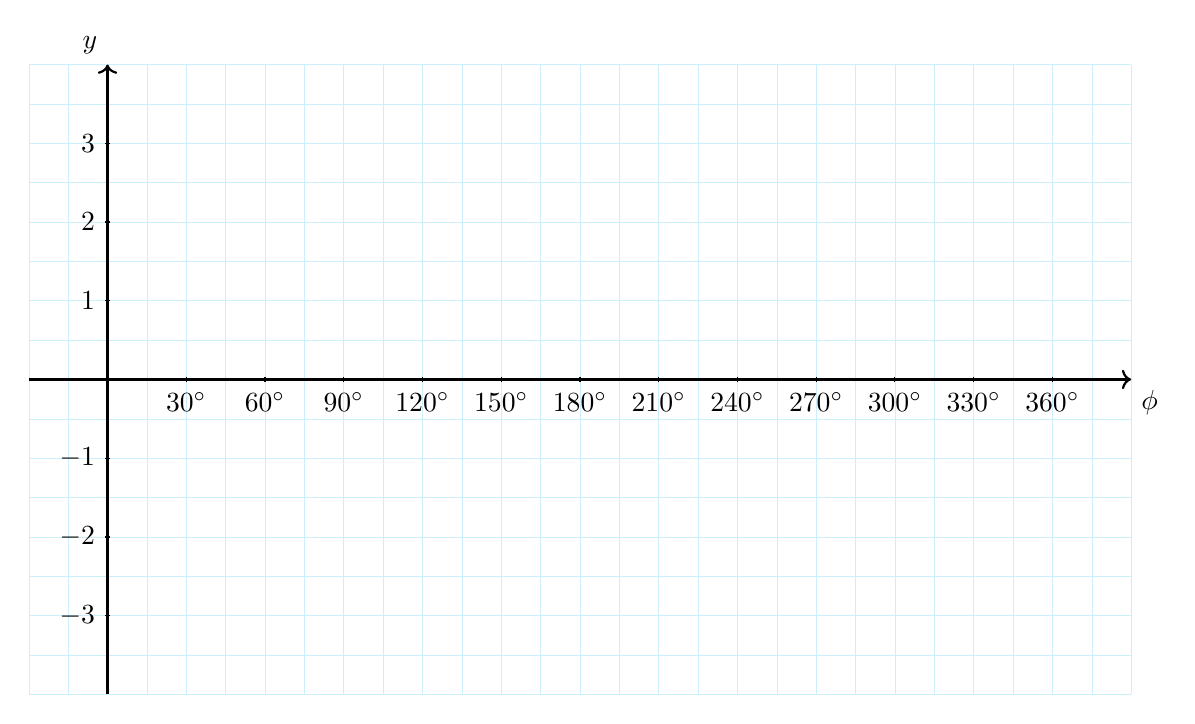
\begin{tikzpicture}
\draw[step = 0.5 cm, cyan!20 , very thin] (-1, -4) grid ( 13, 4);
\draw[thick, ->] (-1,0) -- (13,0) node[anchor = north west] {$\phi$};
\draw[thick, ->] (0,-4) -- (0,4) node[anchor = south east] {$y$};

\foreach \x [evaluate=\x as \degree using int(\x*30)] in {1,...,12}{ 
   \draw (\x cm, 1pt) -- (\x cm, -1pt) node[anchor = north] {$\degree^\circ$};
   }
\foreach \y in {-3,-2,-1,1,2,3}
   \draw (1pt, \y cm) -- (-1pt, \y cm) node[anchor = east] {$\y$};
\end{tikzpicture}}%% END Definition

\newcommand{\trigsysB}{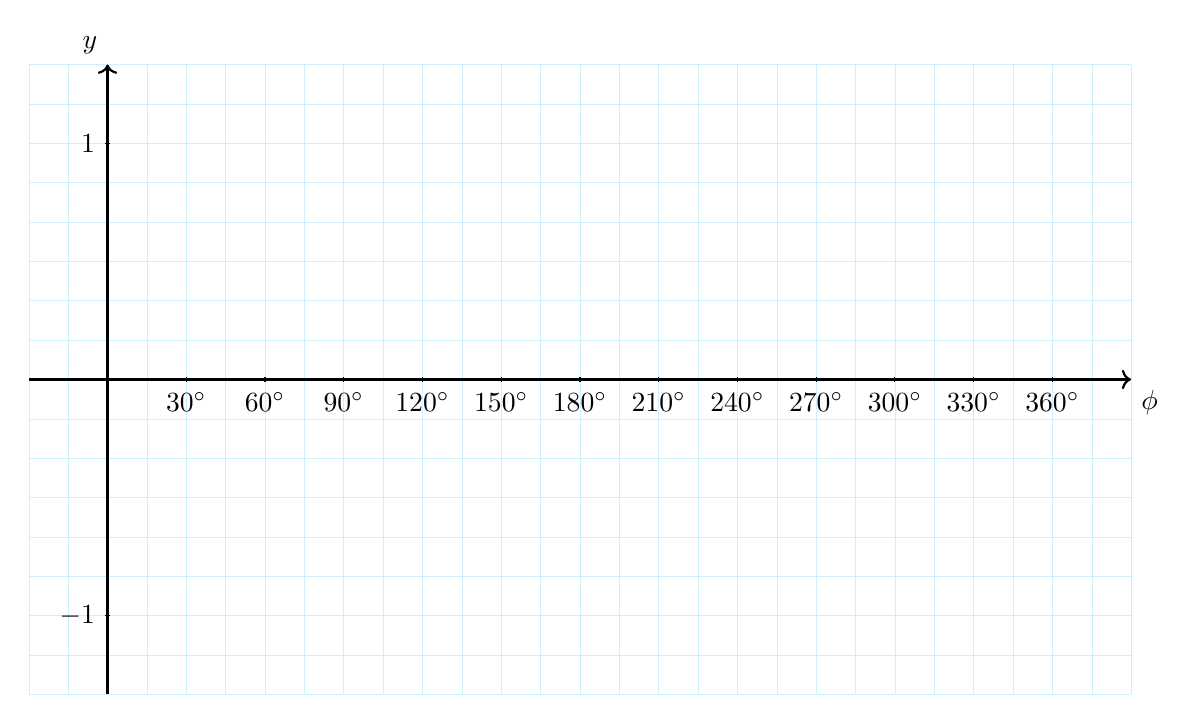
\begin{tikzpicture}\draw[step = 0.5 cm, cyan!20 , very thin] (-1, -4) grid ( 13, 4);
\draw[thick, ->] (-1,0) -- (13,0) node[anchor = north west] {$\phi$};
\draw[thick, ->] (0,-4) -- (0,4) node[anchor = south east] {$y$};

\foreach \x [evaluate=\x as \degree using int(\x*30)] in {1,...,12}{ 
   \draw (\x cm, 1pt) -- (\x cm, -1pt) node[anchor = north] {$\degree^\circ$};
   }
\foreach \y in {-1,1}
   \draw (1pt, \y *3cm) -- (-1pt, \y *3cm) node[anchor = east] {$\y$};

\end{tikzpicture}}%% END Definition

\newcommand{\trigsysC}{
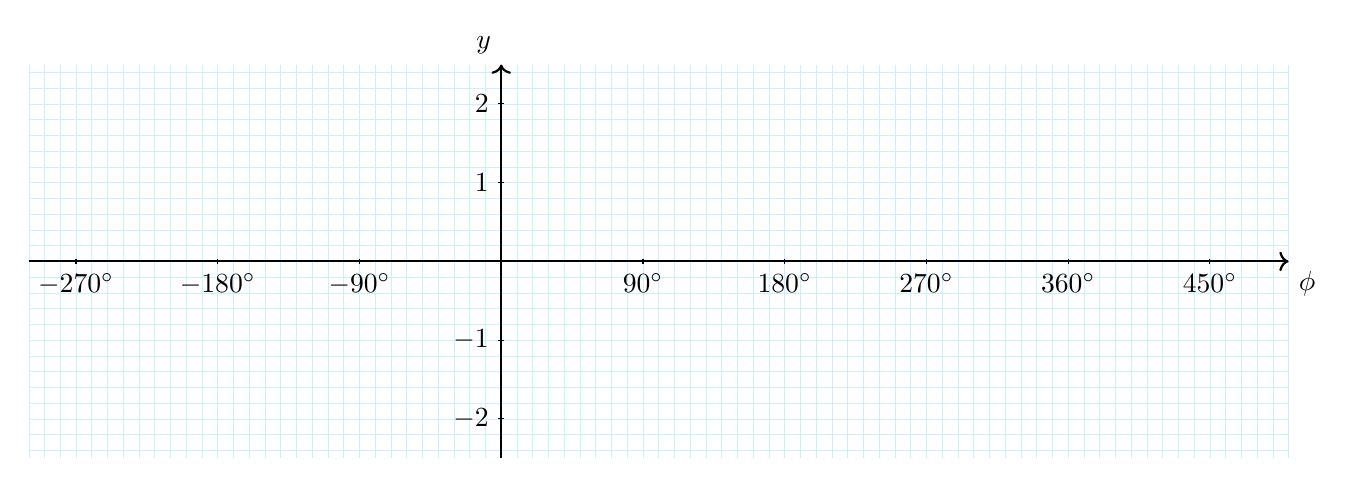
\begin{tikzpicture}
\draw[step = 0.2 cm, very thin, cyan!20] (-6, -2.5) grid ( 10, 2.5);
\draw[thick, ->] (-6,0) -- (10,0) node[anchor = north west] {$\phi$};
\draw[thick, ->] (0,-2.5) -- (0,2.5) node[anchor = south east] {$y$};

\foreach \x [evaluate=\x as \degree using int(\x*90)] in {-3,-2,-1,1,2,3,4,5}{ 
   \draw (\x *18mm, 1pt) -- (\x * 18mm, -1pt) node[anchor = north] {$\degree^\circ$};
   }
   
\foreach \y in {-2,-1,1,2}
   \draw (1pt, \y cm) -- (-1pt, \y cm) node[anchor = east] {$\y$};
\end{tikzpicture}}%% END Definition

\newcommand{\trigsysD}{
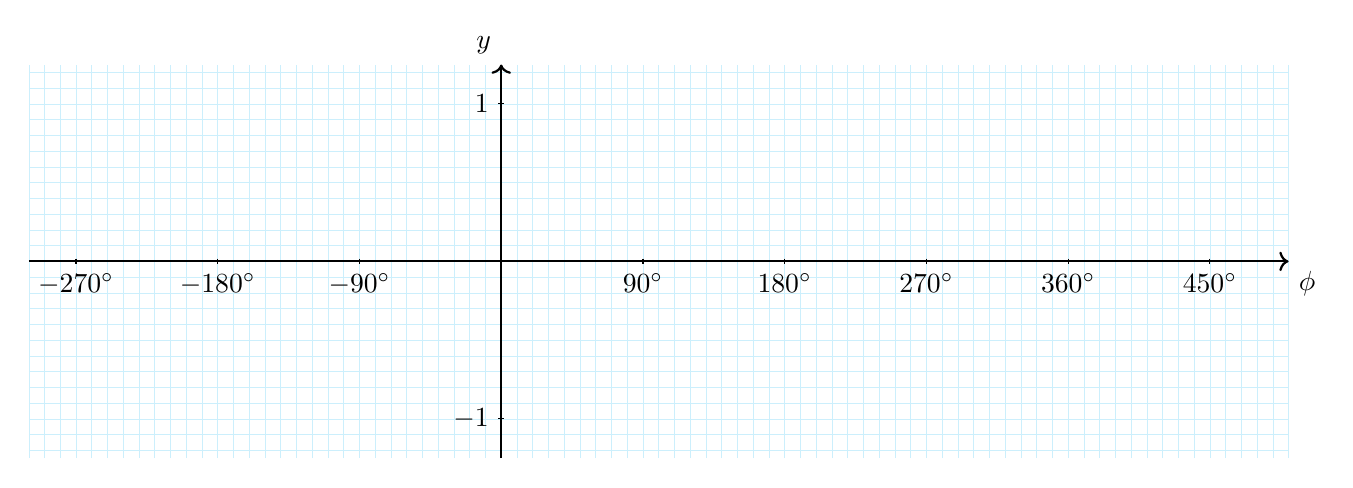
\begin{tikzpicture}
\draw[step = 0.2 cm, very thin, cyan!20] (-6, -2.5) grid ( 10, 2.5);
\draw[thick, ->] (-6,0) -- (10,0) node[anchor = north west] {$\phi$};
\draw[thick, ->] (0,-2.5) -- (0,2.5) node[anchor = south east] {$y$};

\foreach \x [evaluate=\x as \degree using int(\x*90)] in {-3,-2,-1,1,2,3,4,5}{ 
   \draw (\x *18mm, 1pt) -- (\x * 18mm, -1pt) node[anchor = north] {$\degree^\circ$};
   }
   
\foreach \y in {-1,1}
   \draw (1pt, \y *2cm) -- (-1pt, \y *2cm) node[anchor = east] {$\y$};
\end{tikzpicture}}%% END Definition


\newcommand{\trigsysDsin}{
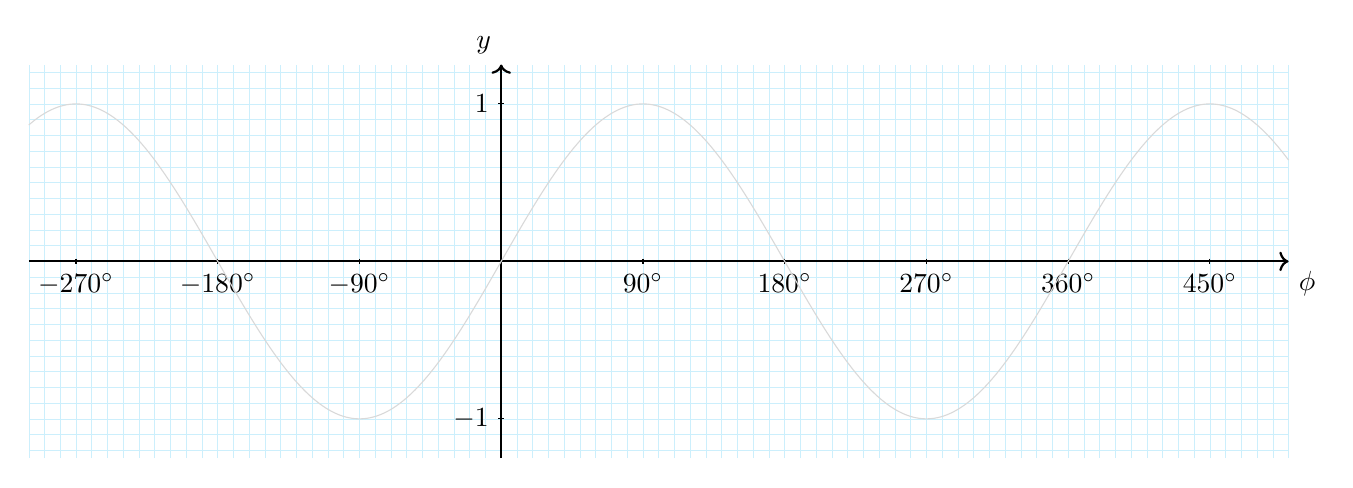
\begin{tikzpicture}
\draw[step = 0.2 cm, very thin, cyan!20] (-6, -2.5) grid ( 10, 2.5);
\draw[thick, ->] (-6,0) -- (10,0) node[anchor = north west] {$\phi$};
\draw[thick, ->] (0,-2.5) -- (0,2.5) node[anchor = south east] {$y$};

\foreach \x [evaluate=\x as \degree using int(\x*90)] in {-3,-2,-1,1,2,3,4,5}{ 
   \draw (\x *18mm, 1pt) -- (\x * 18mm, -1pt) node[anchor = north] {$\degree^\circ$};
   }
   
\foreach \y in {-1,1}
   \draw (1pt, \y *2cm) -- (-1pt, \y *2cm) node[anchor = east] {$\y$};

\draw[domain=-6:10,smooth,samples=200,variable=\x,gray!30] plot ({\x},{2*sin(\x*50)});
\end{tikzpicture}}%% END Definition

\newcommand{\trigsysDcos}{
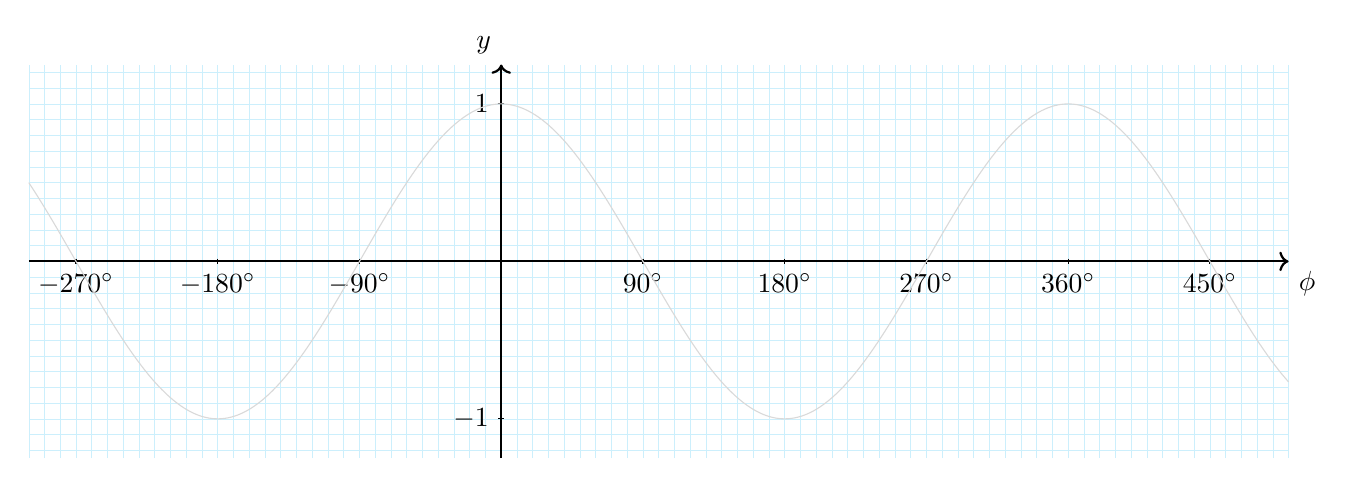
\begin{tikzpicture}
\draw[step = 0.2 cm, very thin, cyan!20] (-6, -2.5) grid ( 10, 2.5);
\draw[thick, ->] (-6,0) -- (10,0) node[anchor = north west] {$\phi$};
\draw[thick, ->] (0,-2.5) -- (0,2.5) node[anchor = south east] {$y$};

\foreach \x [evaluate=\x as \degree using int(\x*90)] in {-3,-2,-1,1,2,3,4,5}{ 
   \draw (\x *18mm, 1pt) -- (\x * 18mm, -1pt) node[anchor = north] {$\degree^\circ$};
   }
   
\foreach \y in {-1,1}
   \draw (1pt, \y *2cm) -- (-1pt, \y *2cm) node[anchor = east] {$\y$};

\draw[domain=-6:10,smooth,samples=200,variable=\x,gray!30] plot ({\x},{2*cos(\x*50)});
\end{tikzpicture}}%% END Definition




\usepackage{bbwLayoutDocSty}

%%%%%%%%%%%%%%%  H E A D E R   &   F O O T E R %%%%%%%%%%%%%%%%%%%%

%% Oben (Header) linke Seite
\fancyhf[HLE]{\makebox{
\includegraphics[width=37mm]{logos/bbwBreit.pdf}}} 
\fancyhf[HCE]{\parttitle}
%% Oben (Header) rechte Seite
\fancyhf[HRO]{\leftmark}
%% Unten (Footer)  FRE = right even, FLE= left even, FRO = right odd,
%% FCO = center odd
\fancyhf[FRE]{\doctitel{}:\ \fachthema}
\fancyhf[FLE,FRO]{\thepage{}/\pageref{LastPage}}
\fancyhf[FCO]{BBW: Abteilung 6 BMS}


\renewcommand{\author}{Philipp G. Freimann}
\renewcommand{\grafikautor}{Ph. G. Freimann}
\renewcommand{\authoremail}{philipp.freimann@bbw.ch}
\renewcommand{\erstellungsdatum}{22. Juni 2022}
\renewcommand{\docversion}{1.2.3 (\LaTeX{})}

%%\renewcommand{\modulnummer}{Arithmetik und Algebra I}
\renewcommand{\doctitel}{Mathematik}
\renewcommand{\fachthema}{Blended Learning}

%%%%%%%%%%%%%%%%%%%%%%%%%%%%%%%%%%%%%%%%%%%%%%%%%%%%%%%%%%%%%%%%%%%%
%% Gesamt-Skripts benötigen ALINONE (all in one), damit Referenzen auf andere
%% Kapitel funktioniren:
\isALLINONEtrue%%
\isBLENDEDtrue%%

\scriptStart{}

%% Einstiegsaufgaben
%%
%% 2019 07 04 Ph. G. Freimann
%%

\section*{Einstiegsaufgaben}
\sectuntertitel{Der Anfang ist die Hälfte des Ganzen (Aristoteles)}
%%%%%%%%%%%%%%%%%%%%%%%%%%%%%%%%%%%%%%%%%%%%%%%%%%%%%%%%%%%%%%%%%%%%%%%%%%%%%%%%%
\GESO{\cite{marthaler21} ab. S. 22}


\subsection*{Abholen des Bekannten und Geübten}

\GESO{
  
  Vereinfachen Sie den Term so weit wie möglich\footnote{Aufgaben aus
    BMS Aufnahmeprüfungen}:
  $$\sqrt{(7x)^2 + 17x^2 - 2x^2}$$

\TNT{3.2}{
  $$\sqrt{49x^2 + 17x^2 - 2x^2}$$
  $$\sqrt{64x^2} = 8x$$
  \vspace{3cm}} %% END TNT

  %%%%%%%%%%%%%%%%%%%%%%%%%%%%%%%%%%55

  Berechnen Sie die Lösung der Gleichung:

  $$x^2 + 11 = (x+3)^2$$

\TNT{7.2}{$$x = \frac{1}{3}$$
\vspace{5cm}
  }


    %%%%%%%%%%%%%%%%%%%%%%%%%%%%%%%%%%55
  \newpage
  Vereinfachen Sie den Term so weit wie möglich:

  $$\frac{4b^2}{2a}:\frac{b^2}{3a^2} - \frac{a}{5}$$

\TNT{7.2}{$$\frac{4b^2}{2a}\cdot{}\frac{3a^2}{b^2} - \frac{a}{5}$$
    $$\frac{4\cdot{}3a}{2} - \frac{a}{5}$$
    $$\frac{60\cdot{}a}{10} - \frac{2a}{10}$$
    $$\frac{58a}{10} = 5.8a$$
\vspace{5cm}
  
}
  \newpage


In einer Schachtel liegen vier grüne und fünf rote Kugeln.
Sie ziehen nacheinander zwei Kugeln, ohne sie wieder zurückzulegen.

a) Zeichnen Sie einen entsprechenden Wahrscheinlichkeitsbaum und tragen Sie die
Wahrscheinlichkeiten bei den Ästen ein.

\TNT{4.8}{\vspace{48mm}}


b) Berechnen Sie die Wahrscheinlichkeit, zwei grüne Kugeln zu ziehen.

\TNT{4.8}{\vspace{48mm}}

%%%%%%%%%%%%%%%%%%%%%%%%%%%%%%%%%%%%%%%%%%%%%%%5
%  Ein Radfahrer fährt von zu Hause zum Arbeitsplatz. Am Anfang fährt
%  er während 15 Minuten mit einer Geschwindigkeit von 30 km/h. An
%  einer Ampel muss er für 3 Minuten anhalten. Anschließend fährt er
%  während 30 Minuten mit einer Geschwindigkeit von 20 km/h bis zum
%  Arbeitsplatz.

%  Was ist die durchschnittliche Geschwindigkeit des Radfahrers von
%  seinem Wohnort bis zur Arbeit in km/h?

%\noTRAINER{  \mmPapier{8.0}}
%  \TRAINER{1. Totale Strecke rechnen (17.5 km). 2. Totale Zeit
%    rechnen: 48 Minuten = 0.8 h. Danach: v = s/t: 21.875km/h.
%    \vspace{5cm}}

}%% END GESO
\newpage


%% Arithmetik und Algebra Grundlagen
\part{Gleichungen II}\index{Gleichungen!II|textbf}
\renewcommand{\bbwPartID}{GL2}
%%  OLAT Arbeitsblatt
\GESO{\olatLinkArbeitsblatt{Potenz- und Wurzelgleichungen}{https://olat.bbw.ch/auth/RepositoryEntry/572162163/CourseNode/101937264586296}{Aufg. Kap. 2.2}}%% END olatLinkArbeitsblatt
\TALS{\olatLinkArbeitsblatt{Potenz- und Wurzelgleichungen}{https://olat.bbw.ch/auth/RepositoryEntry/572162090/CourseNode/105177901239296}{Aufg. Kap. 2.2}}%% END olatLinkArbeitsblatt
%%
%% 2019 07 04 Ph. G. Freimann
%%

\section{Potenz- und Wurzelgleichungen}\index{Gleichungen!mit Potenzen}\index{Potenzgleichungen}\index{Wurzelgleichungen}\index{Gleichungen!mit Wurzeln}

\theorieGESO{191}{11}
%%\theorieTALS{}{}
%%%%%%%%%%%%%%%%%%%%%%%%%%%%%%%%%%%%%%%%%%%%%%%%%%%%%%%%%%%%%%%%%%%%%%%%%%%%%%%%%
\subsection*{Lernziele}

\begin{itemize}
\item Potenzgleichungen
\item Wurzelgleichungen
\end{itemize}
\newpage

%%
%% 2020 05 07 Ph. G. Freimann
%%

%% Überblick über die Begriffe
%% Potenz, Potenzgleichung, Exponentialgleichung, Wurzelgleichung

\subsection{Überblick über Gleichungen mit Potenzen}

\begin{tabular}{|p{52mm}|p{52mm}|p{52mm}|}
  \hline
  Potenzwert gesucht       & Basis gesucht                       &  Exponent gesucht          \\
  \hline
  $10^3=x$                 & $x^3=1000$                           &  $10^x=1000$               \\
  \hline
  $x=10\cdot{}10\cdot{}10$ & $x=\sqrt[3]{1000}$                   & $x =  \log_{10}(1000)$     \\
  $x=1000$                 & $x=10$                               & $x =  3$                   \\
                           & Potenzgleichung                      & Exponentialgleichung       \\



  \hline
  \multicolumn{3}{c}{\,}\\ %% Generiere etwas Abstand
  \multicolumn{3}{c}{Beispiel Zweierpotenzen}\\
  \hline
  Potenz                   & Potenzgleichung bzw. Wurzelgleichung &  Exponentialgleichung     \\
  \hline 
  $2^5=x$                  & $x^5=32$                             &  $2^x=32$                  \\
  \hline
  $x=2\cdot{}2\cdot{}2\cdot{}2\cdot{2}$ & $x=\sqrt[5]{32}$        & $x =  \log_{2}(32)$        \\
  $x=32$                   & $x=2$                                & $x  =  3$                  \\
  \hline


  \hline
  \multicolumn{3}{c}{\,}\\ %% Generiere etwas Abstand
  \multicolumn{3}{c}{\GESO{(Optional)}\TALS{Erinnerung} --- Wurzeln sind rationale Exponenten:}\\
  \hline
  Wurzelwert gesucht        & Radikand gesucht                   &  Wurzelexponent gesucht            \\
  \hline
  $\sqrt[3]{1000}=x$        & $\sqrt[3]{x}=10$                    &  $\sqrt[x]{1000}=10$               \\
  \hline
  $1000^{\frac{1}{3}}=x$     & $x^{\frac{1}{3}}=10$                   &  $1000^{\frac{1}{x}}=10$               \\
  $x=\sqrt[3]{1000}$       & $x=10^3$                             & $\frac{1}{x} =  \log_{1000}(10)$      \\
  $x=10$                   & $x=1000$                             & $\frac{1}{x} =  \frac{1}{3}$         \\
                           &                                      & $x = 3$                      \\\hline
\end{tabular}

\GESO{Bem. zum Logarithmus zur Basis 2 ($\log_{2}(32)$): Dazu müssen
  Sie die

  \tiprobutton{ln_log}-Taste
 auf Ihrem TI-30 Taschenrechner 3x drücken.}

\newpage


\subsection{Potenzgleichung}\index{Potenzgleichungen}
\begin{definition}{Potenzgleichung}{}
  Bei \textbf{Potenzgleichungen}\index{Potenzgleichung}\footnote{Potenzgleichungen sind nicht zu
  verwechseln mit Exponentialgleichungen, bei denen das $x$ im
  Exponenten steht: $5^{2x-1}=7$} ist die Gesuchte ($x$) in der Basis
  einer Potenz.
\end{definition}

Im folgenden Beispiel kommt $x$ in der 5-ten Potenz vor:

$$x^5 = 1024$$

Typischerweise löst man diese Gleichungen mit der $n$-ten Wurzel.

\TNT{4}{
\begin{tabular}{rccl}
  \             & $x^5$           &=& 1024             \\
  $\Rightarrow$ & $\sqrt[5]{x^5}$ &=& $\sqrt[5]{1024}$ \\
  $\Rightarrow$ & $x$             &=& $4$ 
\end{tabular}
}%% END TNT

Was ist die Lösungsmenge der folgenden Potenzgleichung?

$$x^2 = 100$$

\TNT{2.4}{%%
$$x^2 = 100 \textrm{ somit } x=\pm\sqrt{100} = \pm 10.$$}%% END TNT

Bestimmen Sie auch die Lösungsmenge der folgenden Gleichung:
$$x^4 = 81$$
\TNT{2.4}{%%
$x^4 = 81$ heißt, $x=\pm \sqrt[4]{81} = \pm 3$
}%% end TNT

\newpage
\subsubsection{Vorzeichen}
Vorsicht ist geboten bei negativen Zahlen.

\begin{gesetz}{}{}
  Gerade Exponenten (2, 4, 6,
8, ...) zwingen die Potenz immer dazu, positiv zu werden. Beispiel:

$$x^6 \ge 0$$

Der Potenzwert bei ungeraden Exponenten hat dasselbe Vorezeichen wie die
Basis.

Beispiel:

$$(-3)^5 = \LoesungsRaumLang{((-1)\cdot{}(3))^5} = \LoesungsRaum{(-1)^5 \cdot 3^5} = - (3^5)$$
\end{gesetz}


Beachten Sie die folgenden typischen Fälle:

 \renewcommand{\arraystretch}{2}

\begin{tabular}{|c|l|}
  \hline
  $x^2 = 4$ & $\lx=\LoesungsRaumLang{\{-2; +2\}}$ \\
  \hline
  $x^3 =  8$& $\lx=\LoesungsRaumLang{\{2\}}$ \\
  \hline
  $x^3 = -8$& $\lx=\LoesungsRaumLang{\{-2\}}$ \\
  \hline
  $x^6 = -5$& $\lx=\LoesungsRaumLang{\{\,\}}$ \\
  \hline
  $x^7 = -5$& $\lx=\LoesungsRaumLang{\{-\sqrt[7]{5}\}}$ \\
  \hline
  \end{tabular} 

 \renewcommand{\arraystretch}{1}

 \newpage
 
\begin{gesetz}{}{}

 \begin{center}\fbox{Gegeben $x^n=a$, $n\ne 0$}\end{center}
 \begin{center}\fbox{Gesucht $\lx$}\end{center}

 \renewcommand{\arraystretch}{2}

 \begin{tabular}{l|l|l}
                        & $a>0$                                  & $a<0$                      \\\hline
  $n$ gerade            & $\lx =\LoesungsRaumLang{\{-\sqrt[n]{a}; +\sqrt[n]{a}\}}$ & $\lx=\LoesungsRaumLang{\{\}}$               \\\hline
  $n$ \textbf{un}gerade & $\lx = \LoesungsRaumLang{\{+\sqrt[n]{a}\}}$               & $\lx = \LoesungsRaumLang{\{-\sqrt[n]{|a|}\}}$
 \end{tabular}  

 \renewcommand{\arraystretch}{1}

\end{gesetz}
Bemerkung zu $a<0$ und $n$ \textbf{un}gerade: Für den TI-Taschenrechner ist $-\sqrt[3]{5} = \sqrt[3]{-5}$.



\subsection*{Aufgaben}


%%  OLAT Arbeitsblatt
\GESO{\olatLinkArbeitsblatt{Potenz- und Wurzelgleichungen}{https://olat.bbw.ch/auth/RepositoryEntry/572162163/CourseNode/101937264586296}{Aufg. Kap. 1 (Bei 1.2 hilft evtl. die Substitution)}}%% END olatLinkArbeitsblatt
\TALS{\olatLinkArbeitsblatt{Potenz- und Wurzelgleichungen}{https://olat.bbw.ch/auth/RepositoryEntry/572162090/CourseNode/105177901239296}{Aufg. Kap. 1 (Bei 1.2 hilft evtl. die Substitution)}}%% END olatLinkArbeitsblatt

\newpage

\subsection{Wurzelgleichungen}\index{Wurzelgleichung}

\TALS{(\cite{frommenwiler17alg} S.111 (Kap. 2.4.2))}

\begin{definition}{Wurzelgleichung}{}
Kommt in der Gleichung die Gesuchte unter der Wurzel vor, so sprechen
wir von einer \textbf{Wurzelgleichung}.
\end{definition}
Einführungsbeispiel:
$$\sqrt[5]{x}=6$$


Dies löst man indem man beide Seiten der Gleichung potenziert:
\TNT{4}{
  
\begin{tabular}{rccl}
  \             & $\sqrt[5]{x}$   &=&     6      \\
  $\Rightarrow$ & $(\sqrt[5]x)^5$ &=&  $6^5$     \\
  $\Rightarrow$ & $x$             &=& $7\,776$ 
\end{tabular}
}%% END TNT

Lösen Sie das folgende Musterbeispiel:
$$\sqrt{x}+1=2x$$
\TRAINER{Das obige Beispiel von M. Rohner zeigt viele Sackgassen und Dinge, auf die man noch achten muss.}

\GESO{Lösungsverfahren im Buch \cite{marthaler21} Seite 192 im roten
  Kasten.}

\platzFuerBerechnungenBisEndeSeite{}

\TRAINER{1. Wurzel separieren
  $$\sqrt{x}=2x-1$$ quadrieren:
  $$x=4x^2-4x+1$$
  $$0=4x^2-5x+1$$
  $$x_{1,2}=\frac{+5 \pm \sqrt{25-16}}{8}$$
  $$\lx={1}$$, denn $\frac{1}{4}$ ist eine durchs Quadrieren erschienene Scheinlösung.}

\newpage
\begin{bemerkung}{Scheinlösung}{}
  
\textbf{Achtung}: Beim \textbf{Radizieren} auf beiden Seiten
einer Gleichung können \textbf{Lösungen} \textbf{verschwinden}.

Beim \textbf{Potenzieren} können (Schein)\textbf{Lösungen}
\textbf{hinzukommen} \GESO{Bsp. S.191 und roter Kasten S. 192
  im \cite{marthaler21}}.
\end{bemerkung}


\GESO{optional:}
\begin{rezept}{Wurzelgleichung lösen}{}
  \begin{enumerate}
  \item Definitionsbereich $\mathbb{D}$ festlegen
  \item Eine Wurzel isolieren (separieren)
  \item Quadrieren
  \item 2. und 3. Schritt wiederholen, bis keine Wurzeln mehr
    vorkommen
  \item Auflösen
  \item Probe:
    \begin{enumerate}
    \item Mit Definitionsbereich $\mathbb{D}$ abgleichen
    \item In ursprüngliche Gleichung einsetzen
    \end{enumerate}
  \end{enumerate}
\end{rezept}
\newpage


\GESO{Optionales}
Beispiel: $2\cdot{}\sqrt{x+1} + 2 = 5 + 2\cdot{}\sqrt{x-2}$

\TNT{16}{\bbwCenterGraphic{16cm}{allg/gleichungen/img/WurzelgleichungLoesungsweg.png}
  \vspace{3cm}
  $$\lx = \left\{\frac{33}{16}\right\}$$}

\subsection*{Aufgaben}
  \TALSAadB{112ff}{339. d) e), 340. c), 342. d), 344. a) b) c) [Tipp
      bei c): Substitution]}

\GESOAadB{
  196 (Wurzelgleichungen)}{2., 3. a)-f),  4. a) c) d) f),
  5. a) c), 6. b),  7. d), 8. c) d) und Textaufgabe 10. a) und b)}

\newpage


\subsection{Spezielle Exponenten}
\subsubsection{negative
  Exponenten}\index{Exponenten!negative}\index{negative Exponenten}
Bei Potenzgleichungen mit negativen Exponenten ist am Einfachsten
folgendes Potenzgesetz anzuwenden:

$$a^{-n} = \frac1{a^n}$$

Beachte, dass es manchmal zwei Lösungen, manchmal keine gibt.

Beispiel:

$$x^{-4} = 16$$

\TNT{6}{
  Potenzgesetz:   $$\frac1{x^4} = 16$$
  Kehrwert: $$x^4 = \frac1{16}$$
  4. Wurzel: $$x=\pm \sqrt[4] {\frac1{16}}=\frac1{\sqrt[4]{2}}$$
$$\lx = \{-\frac12; \frac12\}$$}%% END TNT

\subsection*{Aufgaben}

%%  OLAT Arbeitsblatt
\GESO{\olatLinkArbeitsblatt{Potenz- und Wurzelgleichungen}{https://olat.bbw.ch/auth/RepositoryEntry/572162163/CourseNode/101937264586296}{Aufg. Kap. 2.1}}%% END olatLinkArbeitsblatt
\TALS{\olatLinkArbeitsblatt{Potenz- und Wurzelgleichungen}{https://olat.bbw.ch/auth/RepositoryEntry/572162090/CourseNode/105177901239296}{Aufg. Kap. 2.1}}%% END olatLinkArbeitsblatt



\newpage

\subsubsection{Rationale Exponenten}\index{Exponenten!rationale}\index{Wurzeln}

 Eine Wurzelgleichung ist nichts anderes als eine
Potenzgleichung mit rationalen Exponenten.

\TRAINER{Anstelle von $\sqrt[n]{x}$ hatten wir auch  $x^{\frac{1}{n}}$
  geschrieben.}

Beispiel: $\sqrt[4]{x^3} = 125$

\TNT{5.2}{

\begin{tabular}{rccl}
%%                & $\sqrt[4]{x^3}$               &=&   125                \\
  $\Rightarrow$ & $x^{\frac{3}{4}}$               &=&   125                \\
  $\Rightarrow$ & $(x^{\frac{3}{4}})^\frac{4}{3}$  &=& $(125)^\frac{4}{3}$  \\
  $\Rightarrow$ & $x^{\frac{3}{4}\cdot\frac{4}{3}}$  &=& $(\sqrt[3]{125})^4$  \\
  $\Rightarrow$ & $x^1$                          &=& $5^4$  \\
  $\Rightarrow$ & $x$                            &=& $625$  
\end{tabular}

}%% END TNT

\subsection*{Aufgaben}

%%  OLAT Arbeitsblatt
\GESO{\olatLinkArbeitsblatt{Potenz- und Wurzelgleichungen}{https://olat.bbw.ch/auth/RepositoryEntry/572162163/CourseNode/101937264586296}{Aufg. Kap. 2.2}}%% END olatLinkArbeitsblatt
\TALS{\olatLinkArbeitsblatt{Potenz- und Wurzelgleichungen}{https://olat.bbw.ch/auth/RepositoryEntry/572162090/CourseNode/105177901239296}{Aufg. Kap. 2.2}}%% END olatLinkArbeitsblatt

\newpage


\section{Exponentialgleichungen}
\matheNinjaLink{Exponentialgleichungen}{https://olat.bbw.ch/auth/RepositoryEntry/667320356/CourseNode/105951756546053}
\bbwCenterGraphic{10cm}{allg/gleichungen/img/Ritter.jpg}
\newpage

%%%%
%% Meta: TI nSpire Einführung
%%       Ziel: Damit die Grundoperationen damit durchgeführt werden können.
%%             Damit man sich an den Rechner gewöhnt.
%%

\input{bmsLayoutPage}
\renewcommand{\bbwAufgabenBlockID}{GL\_Ex}

%%%%%%%%%%%%%%%%%%%%%%%%%%%%%%%%%%%%%%%%%%%%%%%%%%%%%%%%%%%%%%%%%%

\usepackage{amssymb} %% für \blacktriangleright

\renewcommand{\metaHeaderLine}{Arbeitsblatt}
\renewcommand{\arbeitsblattTitel}{Exponentialgleichungen}


\ifisNURAUFGABEN
\renewcommand{\abplz}[1]{\vspace{1mm}}
\fi


\newcommand{\seitenUmbruchImAufgabenteil}{
\ifisNURAUFGABEN
\else
\noTRAINER{\newpage}
\fi
}%%



\begin{document}%%
\arbeitsblattHeader{} (V 1.7 2025-10-18)

\section{Exponentenvergleich}

% \newcommand{\plz}{\noTRAINER{\\ \mmPapier{5.2}}}

Lösen Sie durch Exponentenvergleich:

\begin{bbwAufgabenBlock}
\item $5^{2x+1} = 5^{x-2}$                        $\Longrightarrow$ $\lx=\LoesungsRaumLang{\{-3\}}$ \abplz{7.2}
\item $7^x \cdot 7^{12} = 7^{21}$                 $\Longrightarrow$ $\lx=\LoesungsRaumLang{\{9\}}$ \abplz{7.2}\noTRAINER{\seitenUmbruchImAufgabenteil{}}
\item $(r^x)^3 \cdot{} r^2 = r^{x+5} \cdot{} r^x$ $\Longrightarrow$ $\lx=\LoesungsRaumLang{\{3\}}$ \abplz{7.2}
\item $a^4 = \frac{a^{3x}}{a^{-6}}$ $\Longrightarrow$ $\lx=\LoesungsRaumLang{\{-\frac23\}}$ \abplz{7.2}\noTRAINER{\seitenUmbruchImAufgabenteil{}}
\item $(f^{-7})^x \cdot{} f^3 = \frac{1}{f^{2x}} : \frac{f^{-1}}{f^{-x}}$ $\Longrightarrow$ $\lx=\LoesungsRaumLang{\{\frac12\}}$ \abplz{7.2}
\item $2^x=32$ $\Longrightarrow$ $\lx=\LoesungsRaumLang{\{5\}}$ \abplz{7.2}\noTRAINER{\seitenUmbruchImAufgabenteil{}}
\item $10^x=0.000\,01$ $\Longrightarrow$ $\lx=\LoesungsRaumLang{\{-5\}}$ \abplz{7.2}
\item $10^{3x}=\sqrt{10}$ $\Longrightarrow$ $\lx=\LoesungsRaumLang{\{\frac16\}}$ \abplz{7.2}\noTRAINER{\seitenUmbruchImAufgabenteil{}}
\item $10^{3x-8}=1$ $\Longrightarrow$ $\lx=\LoesungsRaumLang{\{\frac83\}}$ \abplz{7.2}
\item $10^{x-2}=1\,000$ $\Longrightarrow$ $\lx=\LoesungsRaumLang{\{5\}}$ \abplz{7.2}\noTRAINER{\seitenUmbruchImAufgabenteil{}}

\item $3^{\frac{x-1}{3}} = \frac1{9^{\frac{x+1}{4}}}$ $\Longrightarrow$ $\lx=\LoesungsRaumLang{\{-\frac15\}}$ \abplz{7.2}
\item $9^x = 8\cdot{}3^x + 3^x$ $\Longrightarrow$ $\lx=\LoesungsRaumLang{\{2\}}$ \abplz{7.2}

\item $10^{x-4}=1000$ $\Longrightarrow$ $\lx=\LoesungsRaumLang{\{7\}}$ \abplz{7.2}

\end{bbwAufgabenBlock}
\newpage
%
%%%%%%%%%%%%%%%%%%%%%%%%%%%%%%%%%%%%%%%%%%%%%%%%%%%%%%%%%%%%%%%%%%%%%%%%%%%%%%%%%%%%%%%%%%%%%%
%
\section{Logarithmieren mit dem Taschenrechner}
Lösen Sie folgende Gleichung durch Logarithmieren und geben Sie die
Resultate einerseits exakt (Brüche, Wurzeln, Logarithmen/Zehnerlogarithmen), andererseits mit
Hilfe des Taschenrechners auf drei oder vier signifikante Stellen an.

Formel
$$\log_b(a) = \frac{\lg(a)}{\lg(b)}$$

\begin{bbwAufgabenBlock}

\item $10^x=1001$ $\Longrightarrow$
$\lx=\LoesungsRaumLang{\{\frac{\lg(1001)}{\lg(10)} = \frac{\lg(1001)}{1} = \lg(1001) \approx 3.00\}}$ \abplz{7.2}\noTRAINER{\seitenUmbruchImAufgabenteil{}}

\item $2^x=30$ $\Longrightarrow$ $\lx=\LoesungsRaumLang{\{\frac{\lg(30)}{\lg(2)}\approx 4.91\}}$ \abplz{7.2}\noTRAINER{\seitenUmbruchImAufgabenteil{}}
\item $13^x=1000$ $\Longrightarrow$ $\lx=\LoesungsRaumLang{\{\frac{\lg(1000)}{\lg(13)}\approx 2.69\}}$ \abplz{7.2}
\item $5\cdot{}7^x = 19$ $\Longrightarrow$ $\lx=\LoesungsRaumLang{\{\frac{\lg(19)-\lg(5)}{\lg(7)}\approx 0.686\}}$ \abplz{7.2}\noTRAINER{\seitenUmbruchImAufgabenteil{}}
\item $7\cdot{}3^x = 2 + 4\cdot{}3^x$ $\Longrightarrow$ $\lx=\LoesungsRaumLang{\{\frac{\lg(2)-\lg(3)}{\lg(3)}\approx  \}}$ \abplz{7.2}
\item $3\cdot{}6^x - 36 = 6^x$ $\Longrightarrow$ $\lx=\LoesungsRaumLang{\{\frac{\lg(18)}{\lg(6)} \approx  1.61 \}}$ \abplz{7.2}\noTRAINER{\seitenUmbruchImAufgabenteil{}}
\item $2^{5x} = 5^{2x}$ $\Longrightarrow$ $\lx=\LoesungsRaumLang{\{0\}}$ \abplz{7.2}
\end{bbwAufgabenBlock}

\newpage

\section{Form $a^{T} = b$}
Bringen Sie die folgenden Gleichungen erst in die Form $a^T=b$, wobei
$T=T(x)$ ein Term in $x$ ist.

\begin{bbwAufgabenBlock}
\item $8\cdot{} 5^{2x+1} = 200$  $\Longrightarrow$ $\lx=\LoesungsRaumLang{\{ 0.5 \}}$ \abplz{7.2}


\item $\frac12 \cdot{} 4^{7x-32} = 32$  $\Longrightarrow$ $\lx=\LoesungsRaumLang{\{ 5 \}}$ \abplz{7.2}\noTRAINER{\seitenUmbruchImAufgabenteil{}}

Lösen Sie exakt von Hand und runden Sie das Resultat anschließend mit dem Taschenrechner auf vier signifikante Stellen.

\item $3.4^{\frac{x}2} = 16$  $\Longrightarrow$
$\lx=\LoesungsRaumLang{\{2\cdot{} \frac{\lg(16)}{\lg(3.4)} \approx 4.531 \}}$ \abplz{7.2}
\noTRAINER{\seitenUmbruchImAufgabenteil{}}
\item $6^{\frac{x}3} = 14$  $\Longrightarrow$
$\lx=\LoesungsRaumLang{\{3\cdot{} \frac{\lg(14)}{\lg(6)} \approx 4.419 \}}$ \abplz{7.2}

\item $1.8^{\frac{x}5+1} = 100$  $\Longrightarrow$
$\lx=\LoesungsRaumLang{\{5\cdot{}\left(\frac{2}{\lg(1.8)} - 1\right) \approx 34.17 \}}$ \abplz{7.2}\noTRAINER{\seitenUmbruchImAufgabenteil{}}


\item $3 = 4 - 5\cdot{}6^\frac{x}7$  $\Longrightarrow$ $\lx=\LoesungsRaumLang{\{ 7\cdot{} \log_{6}\left(\frac{3-4}{-5}\right)  \approx  -6.288 \}}$ \abplz{7.2}

\item $8 = 7 + 6\cdot{}5^\frac{x}4$  $\Longrightarrow$ $\lx=\LoesungsRaumLang{\{ 4\cdot{} \log_{5}\left(\frac{8-7}{6}\right)  \approx -4.453 \}}$ \abplz{7.2}\noTRAINER{\seitenUmbruchImAufgabenteil{}}

\item $40 = 50 - 40\cdot{}0.8^\frac{t}7$  $\Longrightarrow$ $\mathbb{L}_t=\LoesungsRaumLang{\{ 7\cdot{} \log_{0.8}\left(\frac{40-50}{-30}\right)  \approx 43.49 \}}$ \abplz{7.2}
\\




\item $1200=3\cdot{} 5^{\frac{t}{4}} \Longrightarrow$ $L_t = \LoesungsRaumLang{\{ 4\cdot{}\log_5(\frac{1200}3)\approx 14.89   \}}$ \abplz{7.2}\noTRAINER{\seitenUmbruchImAufgabenteil{}}

\item $0.93^{\frac{t}4}=\frac12 \Longrightarrow$ $L_t
= \LoesungsRaumLang{\{
4\cdot{}\log_{0.93}\left(\frac12\right) \approx 38.205   \}}$ \abplz{7.2}

\noTRAINER{\seitenUmbruchImAufgabenteil{}}

\item $28 = 4 + 3\cdot{} 2^\frac{t}{4} \Longrightarrow$ $L_t
= \LoesungsRaumLang{\{ 4\cdot{} \log_2\left(\frac{28-4}3\right) = 12 \}}$ \abplz{7.2}


\item $4.7 = 8 - 0.6\cdot{} 1.25^{\frac{t}{3}} \Longrightarrow$ $L_t
= \LoesungsRaumLang{\{
3\cdot{} \log_{1.25}\left(\frac{4.7-8}{-0.6}\right) \approx 22.9191  \}}$ \abplz{7.2}

\noTRAINER{\seitenUmbruchImAufgabenteil{}}


Lösen Sie von Hand:

\item $5 \cdot{} 3^{\frac{7-x}{2}} = 45$  $\Longrightarrow$ $\lx=\LoesungsRaumLang{\{  3   \}}$ \abplz{7.2}

\item $39 =  6\cdot{} 2 ^{5\cdot{} \lg(x) - 7} - 9$  $\Longrightarrow$ $\lx = \LoesungsRaumLang{\{ 100 \}}$ \abplz{7.2}
\noTRAINER{\seitenUmbruchImAufgabenteil{}}

Lassen Sie das exakte Resultat stehen:

\item $5^{\lg(x)+2} = 100$  $\Longrightarrow$ $\lx=\LoesungsRaumLang{\{  10^{\log_5(100)-2}   \}}$ \abplz{7.2}



\end{bbwAufgabenBlock}

\platzFuerBerechnungenBisEndeSeite{}
\newpage
%%%%%%%%%%%%%%%%%%%%%%%%%%%%%%%%%%%%%%%%%%%%%%%%%%%%%%%%%%%%%%%%%%%%%%%%%%%%%%%%%%%%%%%%%%%%%%

\section{Verschiedene Basen}

$$\log(a^n) = n\cdot{}\log(a)$$

Geben Sie auch in folgenden Aufgaben die Lösungen exakt (Wurzeln,
Brüche, Logarithmen) an; aber auch mit Hilfe des Taschenrechners auf drei
signifikante Stellen.

\begin{bbwAufgabenBlock}
\item $3^x=2^{x+2}$ $\Longrightarrow$ $\lx=\LoesungsRaumLang{\{\frac{2\cdot{}\lg(2)}{\lg(3)-\lg(2)} \approx  3.42  \}}$ \abplz{7.2}
\item $7^x=8\cdot{}6^{x+1}$ $\Longrightarrow$ $\lx=\LoesungsRaumLang{\{\frac{\lg(48)}{\lg(7)-\lg(6)} \approx 25.1   \}}$ \abplz{7.2}\noTRAINER{\seitenUmbruchImAufgabenteil{}}
\item $2\cdot{}3^{x+7}=4\cdot{}6^{x+5}$ $\Longrightarrow$ $\lx=\LoesungsRaumLang{\{\frac{\lg(\frac{4\cdot{}6^5}{2\cdot{}3^7})}{\lg(\frac12)} \approx  -2.83  \}}$ \abplz{7.2}
\item $5^{x-1}\cdot{}2^{1-x}=6^{2x}$ $\Longrightarrow$ $\lx=\LoesungsRaumLang{\{\frac{\lg(5)-\lg(2)}{\lg(5)-\lg(2)-2\lg(6)} \approx -0.344   \}}$ \abplz{7.2}\noTRAINER{\seitenUmbruchImAufgabenteil{}}
\item $10\cdot{}3^{4x} = 6^{1-x}\cdot{}4^{3x}$ $\Longrightarrow$ $\lx=\LoesungsRaumLang{\{\frac{\lg(6)-\lg(10)}{\lg(6\cdot{}3^4 - \lg(4^3))} \approx -0.252   \}}$ \abplz{7.2}
\end{bbwAufgabenBlock}

%\platzFuerBerechnungenBisEndeSeite{}
\noTRAINER{\seitenUmbruchImAufgabenteil{}}
%%%%%%%%%%%%%%%%%%%%%%%%%%%%%%%%%%%%%%%%%%%%%%%%%%%%%%%%%%%%%%%%%%%%%%%%%%%%%%%%%%%%%%%%%%%%%%

\section{Logarithmus Naturalis}
Geben Sie die Lösung einerseits mit dem «Logarithmus Naturalis»
($=\ln() = \log_{\e}()$) an, berechnen Sie zur Sicherheit aber auch das
Resultat auf drei signifikante Stellen.

\begin{bbwAufgabenBlock}
\item $4^x=7^{x+2}$ $\Longrightarrow$ $\lx=\LoesungsRaumLang{\{\frac{2\cdot{}\ln(7)}{\ln(4)-\ln(7)} \approx -6.95   \}}$ \abplz{7.2}
\item $\left(\frac14\right)^{3x-1} = \left(\frac15\right)^{2-x}$ $\Longrightarrow$ $\lx=\LoesungsRaumLang{\{\frac{-2\ln(5)-\ln(4)}{-3\ln(4)-\ln(5)} \approx 0.798   \}}$ \abplz{7.2}\noTRAINER{\seitenUmbruchImAufgabenteil{}}
\item $12^x+4\cdot{}3^{4-x}=0$ $\Longrightarrow$
$\lx=\LoesungsRaumLang{\{   \}}$  \abplz{7.2} 
\item $2^{x+1}=5^x + 5^{x-1}$ $\Longrightarrow$ $\lx=\LoesungsRaumLang{\{\frac{\ln(3)-\ln(5)}{\ln(2)-\ln(5)} \approx 0.554   \}}$ \abplz{7.2} \noTRAINER{\seitenUmbruchImAufgabenteil{}}
\item $2^r=3\cdot{}2^{r-3} + 12\cdot{}5^{r-3} - 2\cdot{}5^{r-2}$ $\Longrightarrow$ $\lx=\LoesungsRaumLang{\{ 4 \}}$ \abplz{7.2}
\item $5^x + 5^{x+2} = 2600$ $\Longrightarrow$ $\lx=\LoesungsRaumLang{\{\frac{\ln(100)}{\ln(5)} \approx 2.86   \}}$ \abplz{7.2} \noTRAINER{\seitenUmbruchImAufgabenteil{}}
\item $7^{2x+1} = 100 + 7^{2x-1}$ $\Longrightarrow$ $\lx=\LoesungsRaumLang{\{\frac{\ln(100) - \ln(7-\frac17)}{2\cdot{}\ln(7)} \approx  0.689  \}}$ \abplz{7.2}
\item $\e^x + \e^{x+1} + \e^{x+2} = 1$ $\Longrightarrow$ $\lx=\LoesungsRaumLang{\{\left(\frac{1}{1+\e+\e^2}\right) \approx -2.41  \}}$ \abplz{7.2}

\end{bbwAufgabenBlock}

\newpage{}%%%\platzFuerBerechnungenBisEndeSeite{}
%%%%%%%%%%%%%%%%%%%%%%%%%%%%%%%%%%%%%%%%%%%%%%%%%%%%%%%%%%%%%%%%%%%%%%%%%%%%%%%%%%%%%%%%%%%%%%

\section{Substitution}
Die folgenden Exponentialgleichungen können mit Hilfe einer geeigneten
Substitution auf quadratische Gleichungen zurückgeführt werden.

\begin{bbwAufgabenBlock}
\item $4^x + 4^{2x} = 20$ $\Longrightarrow$ $\lx=\LoesungsRaumLang{\{  1   \}}$ \abplz{7.2}
\item $2\cdot{}5^{2r} = 3.6\cdot{}5^r - 1$ $\Longrightarrow$
$\lx=\LoesungsRaumLang{\left\{   \frac{\ln\left(\frac{9\pm\sqrt{31}}{10}\right)}{\ln(5)} \approx
0.234; -0.664 \right\}
}$\abplz{7.2}

\noTRAINER{\seitenUmbruchImAufgabenteil{}}
%%\noTRAINER{\mmPapier{10}\seitenUmbruchImAufgabenteil{}}

\item $10^x - 10^{-x} = 1$ $\Longrightarrow$ $\lx=\LoesungsRaumLang{\left\{  \frac{\ln\left(\frac{1+\sqrt{5}}{2}\right)}{\ln(10)} \approx  0.209   \right\}}$ 

\end{bbwAufgabenBlock}
\platzFuerBerechnungenBisEndeSeite{}

%%\platzFuerBerechnungenBisEndeSeite{}
%%%%%%%%%%%%%%%%%%%%%%%%%%%%%%%%%%%%%%%%%%%%%%%%%%%%%%%%%%%%%%%%%%%%%%%%%%%%%%%%%%%%%%%%%%%%%%
\seitenUmbruchImAufgabenteil{}
\section{In Textform}
\subsection{Kapital I}
Ein Kapital von CHF $22\,000.-$ wird zu $3.5\%$ Jahreszins angelegt.
\begin{bbwAufgabenBlock}
\item Auf welchen Betrag ist das Kapital nach 7 Jahren
angewachsen?\TRAINER{ 27 990.14 CHF} \abplz{7.2}
\item Auf welchen Betrag ist das Kapital nach 50 Jahren
angewachsen? \TRAINER{ 122868.39 CHF} \abplz{7.2}
\item Auf welchen Betrag ist das Kapital nach $n$ Jahren
angewachsen? \TRAINER{  $22\,000\cdot{} 1.035^n$} \abplz{7.2} \noTRAINER{\seitenUmbruchImAufgabenteil{}}
\item Nach wie vielen Jahren wird das Kapital auf $31\,000.-$ CHF
angewachsen sein? \TRAINER{ 9.97 Jahre} \abplz{7.2}
\end{bbwAufgabenBlock}
\platzFuerBerechnungenBisEndeSeite{}
%%%%%%%%%%%%%%%%%%%%%%%%%%%%%%%%%%%%%%%%%%%%%%%%%%%%%%%%%%%%%%%%%%%%%%%%%%%%%%%%%%%%%%%%%%%%%%
\subsection{Kapital II}
Ein Kapital von CHF $13\,000.-$ wird zu $0.3\%$ jährlichem Zins angelegt.
\begin{bbwAufgabenBlock}
\item Auf welchen Betrag ist das Kapital nach 4 Jahren
angewachsen? \TRAINER{ 13\,156.70 CHF} \abplz{7.2}
\item Auf welchen Betrag ist das Kapital nach 10 Jahren
angewachsen? \TRAINER{ 13\,395.31 CHF} \abplz{7.2}
\item Auf welchen Betrag ist das Kapital nach $n$ Jahren
angewachsen? \TRAINER{ $13\,000\cdot{} 1.003^n$} \abplz{7.2} \noTRAINER{\seitenUmbruchImAufgabenteil{}}
\item Nach wie vielen Jahren wird das Kapital auf $15\,000.-$ CHF
angewachsen sein? \TRAINER{ Nach 47.8 Jahren.} \abplz{7.2}
\end{bbwAufgabenBlock}
\platzFuerBerechnungenBisEndeSeite{}
%%%%%%%%%%%%%%%%%%%%%%%%%%%%%%%%%%%%%%%%%%%%%%%%%%%%%%%%%%%%%%%%%%%%%%%%%%%%%%%%%%%%%%%%%%%%%%
\subsection{Abschreibung}
Ein Computer verliert jedes Jahr um 21\% an Wert. Anfänglich wurde ein Modell «X»
zum Neupreis von 9 870.- eingekauft.

\begin{bbwAufgabenBlock}
\item  Wie viel Wert hat der Computer (Modell «X») nach 3 Jahren
noch? \TRAINER{ 4866.29 CHF } \abplz{7.2}
\item Wie viel Wert hat der Computer nach 15 Jahren noch? \TRAINER{
287.56 CHF} \abplz{7.2}
\item Wie viel Wert hat der Computer nach n Jahren? \TRAINER{ $ 0.79^n \cdot 9870.-$ } \abplz{7.2} \noTRAINER{\seitenUmbruchImAufgabenteil{}}
\item Wann ist der Wert des Computers auf einen Wert von 10\% des
Neuwertes gesunken? \TRAINER{ 9.77 Jahre} \abplz{7.2}
\item Wann hat der Wert des Computer 60\% des Neuwertes
verloren? \TRAINER{ 3.89 Jahre} \abplz{7.2}
\end{bbwAufgabenBlock}

\platzFuerBerechnungenBisEndeSeite{}
%%%%%%%%%%%%%%%%%%%%%%%%%%%%%%%%%%%%%%%%%%%%%%%%%%%%%%%%%%%%%%%%%%%%%%%%%%%%%%%%%%%%%%%%%%%%%%
\subsection{Mille Feuilles}
Blätterteig heißt auf französisch «mille feuilles» (wörtlich also
«tausend Blätter»).

Um Blätterteig herzustellen wird ein Stück Teig halbiert, eingebuttert
und die beiden Hälften werden aufeinander gelegt. Das entstandene
Teigstück wird mit dem Wallholz (Nudelholz) flach ausgewallt und der
Prozess beginnt nach dem Auskühlen von vorn.

Nach dem zweiten Durchgang sind also bereits 4 Schichten übereinander.

\begin{bbwAufgabenBlock}
\item Wie viele Schichten («Blätter») sind nach fünf Durchgängen
vorhanden? \TRAINER{32 «Blätter» sind nach fünf Durchgängen
vorhanden.} \abplz{7.2}

\item Wie viele «Blätter» sind nach $n$ Durchgängen
vorhanden? \TRAINER{Nach $n$ Durchgängen sind es $2^n$ Schichten
vorhanden.} \abplz{7.2}

\item Nach wie vielen Durchgängen sind es tatsächlich tausend
Schichten, sodass «mille feuilles» seinem Namen gerecht
wird? \TRAINER{Nach 10 Durchgängen sind es 1000 (exakt 1024)
Schichten. Rechnung: $$2^n=1000 \Longrightarrow   n
= \log_2(1000) \approx 9.966 $$}

\end{bbwAufgabenBlock}

\platzFuerBerechnungenBisEndeSeite{}
%%%%%%%%%%%%%%%%%%%%%%%%%%%%%%%%%%%%%%%%%%%%%%%%%%%%%%%%%%%%%%%%%%%%%%%%%%%%%%%%%%%%%%%%%%%%%%
\TRAINER{\newpage}
\subsection{Wäldchen}
Ein Wäldchen wächst jedes Jahr um 15\% Waldfläche. (Die anfängliche Fläche werde mit
100\% bezeichnet.)
\begin{bbwAufgabenBlock}
\item Auf wie viel \% ist der Wald nach 5 Jahren angewachsen? \TRAINER{ 201\%} \abplz{7.2}
\item Um wie viel \% ist der Wald nach 5 Jahren angewachsen? \TRAINER{ 101\%} \abplz{7.2}
\item Auf wie viel \% ist der Wald nach n Jahren
angewachsen? \TRAINER{ $1.15^n [\cdot{} 100\%]$} \abplz{7.2} \noTRAINER{\seitenUmbruchImAufgabenteil{}}
\item Nach wie vielen Jahren hat sich die Waldfläche
verdreifacht? \TRAINER{ 7.86 Jahre} \abplz{7.2}
\item Nach wie vielen Jahren sind 100\% Waldfläche
dazugekommen? \TRAINER{nach 4.96 Jahren } \abplz{7.2}
\end{bbwAufgabenBlock}

\platzFuerBerechnungenBisEndeSeite{}
\end{document}


%%%%
%% 2019 07 04 Ph. G. Freimann
%%

\newpage
\section{Textaufgaben/Zinsrechnung}\index{Textaufgaben zur Zinsrechnung}
\sectuntertitel{``Klar hab' ich Probleme --- ich bin Mathelehrer.''}
%%%%%%%%%%%%%%%%%%%%%%%%%%%%%%%%%%%%%%%%%%%%%%%%%%%%%%%%%%%%%%%%%%%%%%%%%%%%%%%%%
\subsection*{Lernziele}

\begin{itemize}
  \item Der Zins ist eine  Multiplikation, der Zinseszins ist eine Potenz
\item Textaufgaben mit Zins und Zinseszins
\end{itemize}

\subsection{Der Zins als Faktor}\index{Zins}
Einstiegsaufgabe:
Ein Händler gibt Ihnen auf eine Ware von 234.50 CHF einen Rabatt von
5\%, wenn Sie sofort bezahlen. Wenn Sie in bar bezahlen, erhalten Sie
einen weiteren Rabatt von 3\%. Ist es für Sie nun schlauer, zuerst den
Sofort-Rabatt (5\%) und danach den Bar-Rabatt(\%) einzufordern oder
ist die umgekehrte Reihenfolge schlauer? \TRAINER{Lsg: 216.10}

\subsubsection{100\% = 1}
Um von einer Ausgangsgröße 100\% zu berechnen, kann einfach der Faktor
1.0 genommen werden. Ebenso kann der Faktor 0.03 genommen werden, um
3\% der Größe zu berechnen. Ein Anwachsen eines Kapitals um 3\% ist
also nichts anderes als das multiplizieren mit dem Faktor 1.03.

\subsubsection{Zinseszins}\index{Zinseszins}
Beim Zinseszins, wird bei jeder weiteren Verzinsung der bereits
erhaltene Zins weiterverzinst. Beispiel 2\%:

CHF 100.- $\rightarrow$ 102.-- $\rightarrow$ 104.04 $\rightarrow$
106.1208

Bei 2\% kann also jedesmal mit einem \textbf{Verzinsungsfaktor} von
1.02 multipliziert werden.
Nach 1000 Jahren wachsen unsere CHF 100.-- also auf $100 *
1.02^{1000}$ an\footnote{Dies entspricht einem Faktor von fast 400 Millionen}. 
\newpage


\subsection{Zinsformel}\index{Zins und Zinseszins}
\TRAINER{Hinweis an die Lehrperson:Insbesondere BM2 gut behandeln, denn der Stoff ist ev. in der Sekundarschule nicht behandelt worden (Sek B) oder es liegt generell zu weit zurück.}

Bei gegebenem Startkapital $K_0$ und gegebenem Zinsfuß $p$ (in \%) kann das Endkapital $K_n$ nach $n$ Jahren wie folgt berechnet werden:

\begin{center}\fbox{$K_n = K_0 \cdot{} f^n$}\end{center}

mit

\begin{center}\fbox{$f := 1 + \frac{p}{100}.$}\end{center}

\begin{tabular}{lcl|l}
  \textit{Zeichen}  & &   \textit{Bedeutung}   & \textit{Beispiel}\\%%
\hline%%
 $K_0$             &=&   Startkapital         & 100.-  [CHF]\\
 $n$               &=&   Laufzeit in Jahren   & 30  [Jahre]\\
 $p$               &=&   Zinsfuß              & 2  [\%]\\
 $f:= 100\% + p\%$ = $1+\frac{p}{100}$ &=&   Zinsfaktor          & hier: $f=1.02$\\
$K_n = K_0\cdot{}f^n$     &=&   Kapital nach $n$ Jahren         & $100 \cdot{} 1.02^{30}\approx{} 181.14$ [CHF]\\%%
\hline\\%%
\end{tabular}

Zeigen Sie, dass gilt

$$K_1 = K_0 + \frac{K_0}{100}\cdot{} p = K_0 \cdot{} \left(1+\frac{p}{100}\right) = K_0 \cdot{} f$$

... und ...:

$$K_2 = K_0 \cdot{} f^2$$

\TNT{4.0}{Beweis: $K_0$ ausklammern. \vspace{3cm}}

Bemerkung: Die Zinseszinsformel beschreibt ein exponentielles Wachstum.
\newpage

\subsubsection{Zinsbeispiele}

Berechnen Sie:

\begin{itemize}
  \item Berechnen Sie das Endkapital nach 20 Jahren bei einem
  Startkapital von CHF 15\,000.- und einem Zins von jährlich
  2.5\%.\\%%

\TNT{2.4}{Endkapital = $15\,000\cdot{} 1.025^{20}\approx 24\,579.25$ CHF\vspace{2cm}}%%
\item In einem Wald werden 200 Fichten für Weihnachten gepflanzt. Wegen der hohen Nachfrage kommen jedes Jahr 3\% Fichten dazu. Wie viele Fichten werden nach fünf Jahren gepfanzt?


  \TNT{2.4}{Endkapital = $200\cdot{} (1.03)^{5} \approx 231$ Fichten.\vspace{2cm}}%%
\item Ein Auto hat einen Neupreis von CHF 40\,000.-. Jedes Jahr müssen wegen Abnutzung ein Wertverlust von 3\% in Kauf
  genommen werden. Wie viel Wert hat das Auto noch nach 15 Jahren? (Achtung, hier ist der Zins negativ!)

\TNT{2.4}{Endkapital = $40\,000\cdot{} (1-0.03)^{15} = 40\,000\cdot{} 0.97^{15}\approx 25\, 330.-$ CHF\vspace{2cm}}
\end{itemize}
\newpage

\subsubsection{Momentanverzinsung}\index{Momentanverzinsung}
(auch stetige Verzinsung)\index{Verzinsung!stetige}
Wird ein Kapital zu 100\% verzinst, so wächst unser Kapital auf 200\%
an. Wenn wir das Kapital jedoch zweimal zu 50\%
verzinsen\footnote{Sprich: Wir lassen uns nach 6 Monaten den Zins
auszahlen, heben das Konto auf und bezahlen sofort wieder mit Zins in
ein neues Konto ein.}, erhalten wir den folgenden, besseren Verzinsungsfaktor:

$1.50^2  = (1 + \frac12)^2 = 2.25$

Bei 4-maliger Verzinsung steigt der Faktor weiter an:
$1.25^4 = (1 + \frac14)^4 \approx 2.44 $

Füllen Sie die folgende Tabelle aus:

\begin{tabular}{c|c|c|c} 
  Anzahl Teile  & Faktor                      & Formel          & Endkapital \\ \hline
  $2$           & $1.5^2$                      & $(1+\frac12)^2$ & $= K_0 \cdot{} 2.25 $ \\ \hline
  $4$           & $1.25^4$                  & $(1+\frac14)^4$ & $\approx K_0 \cdot{} 2.4414 $ \\ \hline
  $5$           & $\LoesungsRaum{1.2^5}$  & $\LoesungsRaum{(1+\frac14)^2}$ & $\LoesungsRaum{= K_0 \cdot{} 2.48832} $ \\ \hline
  $10$           & $\LoesungsRaum{1.1^{10}}$  & $\LoesungsRaum{(1+\frac{1}{10})^{10}}$ & $\LoesungsRaum{\approx K_0 \cdot{} 2.5937} $ \\ \hline
  $100$           & $\LoesungsRaum{1.01^{100}}$  & $\LoesungsRaum{(1+\frac{1}{100})^{100}}$ & $\LoesungsRaum{\approx K_0 \cdot{} 2.7048 }$ \\ \hline
  $1000$           & $\LoesungsRaum{1.001^{1000}}$  & $\LoesungsRaum{(1+\frac{1}{1000})^{1000}}$ & $\LoesungsRaum{\approx K_0 \cdot{} 2.7169 }$ \\ \hline
  Großes $n$           & ****  & $\LoesungsRaum{(1+\frac{1}{n})^{n}}$ & $\LoesungsRaum{\approx K_0 \cdot{} e }$ \\ \hline
\end{tabular} 

Dieses maximal erreichbare Kapital entspricht etwa dem Faktor 2.71828 und
wird als Eulersche Konstante\index{Eulersche Zahl} bezeichnet.

\bbwCenterGraphic{10cm}{allg/img/euler_banknote.jpg}
Bildlegende: Leonhard Euler (1707-1783) auf der Schweizer Zehnernote.

\begin{definition}{Eulersche Zahl}{}
$$e \approx 2.71828182746$$
\end{definition}
\newpage

\GESO{\subsection*{Aufgaben}}
\TALSAadB{???}{???}

\GESOAadB{207}{10. a)} %% die anderen setzen Lograithmen voraus! und 12.}

\GESOAadB{207}{9. a) und 11. a)}
\GESOAadB{355}{13.}
 %% neu bei Potenzen!
\newpage


%%%%%%%%%%%%%%%%
% Gleichungen I
\part{Gleichungen II}\index{Gleichungen!II|textbf}
\renewcommand{\bbwPartID}{GL2}
%%  OLAT Arbeitsblatt
\GESO{\olatLinkArbeitsblatt{Potenz- und Wurzelgleichungen}{https://olat.bbw.ch/auth/RepositoryEntry/572162163/CourseNode/101937264586296}{Aufg. Kap. 2.2}}%% END olatLinkArbeitsblatt
\TALS{\olatLinkArbeitsblatt{Potenz- und Wurzelgleichungen}{https://olat.bbw.ch/auth/RepositoryEntry/572162090/CourseNode/105177901239296}{Aufg. Kap. 2.2}}%% END olatLinkArbeitsblatt
%%
%% 2019 07 04 Ph. G. Freimann
%%

\section{Potenz- und Wurzelgleichungen}\index{Gleichungen!mit Potenzen}\index{Potenzgleichungen}\index{Wurzelgleichungen}\index{Gleichungen!mit Wurzeln}

\theorieGESO{191}{11}
%%\theorieTALS{}{}
%%%%%%%%%%%%%%%%%%%%%%%%%%%%%%%%%%%%%%%%%%%%%%%%%%%%%%%%%%%%%%%%%%%%%%%%%%%%%%%%%
\subsection*{Lernziele}

\begin{itemize}
\item Potenzgleichungen
\item Wurzelgleichungen
\end{itemize}
\newpage

%%
%% 2020 05 07 Ph. G. Freimann
%%

%% Überblick über die Begriffe
%% Potenz, Potenzgleichung, Exponentialgleichung, Wurzelgleichung

\subsection{Überblick über Gleichungen mit Potenzen}

\begin{tabular}{|p{52mm}|p{52mm}|p{52mm}|}
  \hline
  Potenzwert gesucht       & Basis gesucht                       &  Exponent gesucht          \\
  \hline
  $10^3=x$                 & $x^3=1000$                           &  $10^x=1000$               \\
  \hline
  $x=10\cdot{}10\cdot{}10$ & $x=\sqrt[3]{1000}$                   & $x =  \log_{10}(1000)$     \\
  $x=1000$                 & $x=10$                               & $x =  3$                   \\
                           & Potenzgleichung                      & Exponentialgleichung       \\



  \hline
  \multicolumn{3}{c}{\,}\\ %% Generiere etwas Abstand
  \multicolumn{3}{c}{Beispiel Zweierpotenzen}\\
  \hline
  Potenz                   & Potenzgleichung bzw. Wurzelgleichung &  Exponentialgleichung     \\
  \hline 
  $2^5=x$                  & $x^5=32$                             &  $2^x=32$                  \\
  \hline
  $x=2\cdot{}2\cdot{}2\cdot{}2\cdot{2}$ & $x=\sqrt[5]{32}$        & $x =  \log_{2}(32)$        \\
  $x=32$                   & $x=2$                                & $x  =  3$                  \\
  \hline


  \hline
  \multicolumn{3}{c}{\,}\\ %% Generiere etwas Abstand
  \multicolumn{3}{c}{\GESO{(Optional)}\TALS{Erinnerung} --- Wurzeln sind rationale Exponenten:}\\
  \hline
  Wurzelwert gesucht        & Radikand gesucht                   &  Wurzelexponent gesucht            \\
  \hline
  $\sqrt[3]{1000}=x$        & $\sqrt[3]{x}=10$                    &  $\sqrt[x]{1000}=10$               \\
  \hline
  $1000^{\frac{1}{3}}=x$     & $x^{\frac{1}{3}}=10$                   &  $1000^{\frac{1}{x}}=10$               \\
  $x=\sqrt[3]{1000}$       & $x=10^3$                             & $\frac{1}{x} =  \log_{1000}(10)$      \\
  $x=10$                   & $x=1000$                             & $\frac{1}{x} =  \frac{1}{3}$         \\
                           &                                      & $x = 3$                      \\\hline
\end{tabular}

\GESO{Bem. zum Logarithmus zur Basis 2 ($\log_{2}(32)$): Dazu müssen
  Sie die

  \tiprobutton{ln_log}-Taste
 auf Ihrem TI-30 Taschenrechner 3x drücken.}

\newpage


\subsection{Potenzgleichung}\index{Potenzgleichungen}
\begin{definition}{Potenzgleichung}{}
  Bei \textbf{Potenzgleichungen}\index{Potenzgleichung}\footnote{Potenzgleichungen sind nicht zu
  verwechseln mit Exponentialgleichungen, bei denen das $x$ im
  Exponenten steht: $5^{2x-1}=7$} ist die Gesuchte ($x$) in der Basis
  einer Potenz.
\end{definition}

Im folgenden Beispiel kommt $x$ in der 5-ten Potenz vor:

$$x^5 = 1024$$

Typischerweise löst man diese Gleichungen mit der $n$-ten Wurzel.

\TNT{4}{
\begin{tabular}{rccl}
  \             & $x^5$           &=& 1024             \\
  $\Rightarrow$ & $\sqrt[5]{x^5}$ &=& $\sqrt[5]{1024}$ \\
  $\Rightarrow$ & $x$             &=& $4$ 
\end{tabular}
}%% END TNT

Was ist die Lösungsmenge der folgenden Potenzgleichung?

$$x^2 = 100$$

\TNT{2.4}{%%
$$x^2 = 100 \textrm{ somit } x=\pm\sqrt{100} = \pm 10.$$}%% END TNT

Bestimmen Sie auch die Lösungsmenge der folgenden Gleichung:
$$x^4 = 81$$
\TNT{2.4}{%%
$x^4 = 81$ heißt, $x=\pm \sqrt[4]{81} = \pm 3$
}%% end TNT

\newpage
\subsubsection{Vorzeichen}
Vorsicht ist geboten bei negativen Zahlen.

\begin{gesetz}{}{}
  Gerade Exponenten (2, 4, 6,
8, ...) zwingen die Potenz immer dazu, positiv zu werden. Beispiel:

$$x^6 \ge 0$$

Der Potenzwert bei ungeraden Exponenten hat dasselbe Vorezeichen wie die
Basis.

Beispiel:

$$(-3)^5 = \LoesungsRaumLang{((-1)\cdot{}(3))^5} = \LoesungsRaum{(-1)^5 \cdot 3^5} = - (3^5)$$
\end{gesetz}


Beachten Sie die folgenden typischen Fälle:

 \renewcommand{\arraystretch}{2}

\begin{tabular}{|c|l|}
  \hline
  $x^2 = 4$ & $\lx=\LoesungsRaumLang{\{-2; +2\}}$ \\
  \hline
  $x^3 =  8$& $\lx=\LoesungsRaumLang{\{2\}}$ \\
  \hline
  $x^3 = -8$& $\lx=\LoesungsRaumLang{\{-2\}}$ \\
  \hline
  $x^6 = -5$& $\lx=\LoesungsRaumLang{\{\,\}}$ \\
  \hline
  $x^7 = -5$& $\lx=\LoesungsRaumLang{\{-\sqrt[7]{5}\}}$ \\
  \hline
  \end{tabular} 

 \renewcommand{\arraystretch}{1}

 \newpage
 
\begin{gesetz}{}{}

 \begin{center}\fbox{Gegeben $x^n=a$, $n\ne 0$}\end{center}
 \begin{center}\fbox{Gesucht $\lx$}\end{center}

 \renewcommand{\arraystretch}{2}

 \begin{tabular}{l|l|l}
                        & $a>0$                                  & $a<0$                      \\\hline
  $n$ gerade            & $\lx =\LoesungsRaumLang{\{-\sqrt[n]{a}; +\sqrt[n]{a}\}}$ & $\lx=\LoesungsRaumLang{\{\}}$               \\\hline
  $n$ \textbf{un}gerade & $\lx = \LoesungsRaumLang{\{+\sqrt[n]{a}\}}$               & $\lx = \LoesungsRaumLang{\{-\sqrt[n]{|a|}\}}$
 \end{tabular}  

 \renewcommand{\arraystretch}{1}

\end{gesetz}
Bemerkung zu $a<0$ und $n$ \textbf{un}gerade: Für den TI-Taschenrechner ist $-\sqrt[3]{5} = \sqrt[3]{-5}$.



\subsection*{Aufgaben}


%%  OLAT Arbeitsblatt
\GESO{\olatLinkArbeitsblatt{Potenz- und Wurzelgleichungen}{https://olat.bbw.ch/auth/RepositoryEntry/572162163/CourseNode/101937264586296}{Aufg. Kap. 1 (Bei 1.2 hilft evtl. die Substitution)}}%% END olatLinkArbeitsblatt
\TALS{\olatLinkArbeitsblatt{Potenz- und Wurzelgleichungen}{https://olat.bbw.ch/auth/RepositoryEntry/572162090/CourseNode/105177901239296}{Aufg. Kap. 1 (Bei 1.2 hilft evtl. die Substitution)}}%% END olatLinkArbeitsblatt

\newpage

\subsection{Wurzelgleichungen}\index{Wurzelgleichung}

\TALS{(\cite{frommenwiler17alg} S.111 (Kap. 2.4.2))}

\begin{definition}{Wurzelgleichung}{}
Kommt in der Gleichung die Gesuchte unter der Wurzel vor, so sprechen
wir von einer \textbf{Wurzelgleichung}.
\end{definition}
Einführungsbeispiel:
$$\sqrt[5]{x}=6$$


Dies löst man indem man beide Seiten der Gleichung potenziert:
\TNT{4}{
  
\begin{tabular}{rccl}
  \             & $\sqrt[5]{x}$   &=&     6      \\
  $\Rightarrow$ & $(\sqrt[5]x)^5$ &=&  $6^5$     \\
  $\Rightarrow$ & $x$             &=& $7\,776$ 
\end{tabular}
}%% END TNT

Lösen Sie das folgende Musterbeispiel:
$$\sqrt{x}+1=2x$$
\TRAINER{Das obige Beispiel von M. Rohner zeigt viele Sackgassen und Dinge, auf die man noch achten muss.}

\GESO{Lösungsverfahren im Buch \cite{marthaler21} Seite 192 im roten
  Kasten.}

\platzFuerBerechnungenBisEndeSeite{}

\TRAINER{1. Wurzel separieren
  $$\sqrt{x}=2x-1$$ quadrieren:
  $$x=4x^2-4x+1$$
  $$0=4x^2-5x+1$$
  $$x_{1,2}=\frac{+5 \pm \sqrt{25-16}}{8}$$
  $$\lx={1}$$, denn $\frac{1}{4}$ ist eine durchs Quadrieren erschienene Scheinlösung.}

\newpage
\begin{bemerkung}{Scheinlösung}{}
  
\textbf{Achtung}: Beim \textbf{Radizieren} auf beiden Seiten
einer Gleichung können \textbf{Lösungen} \textbf{verschwinden}.

Beim \textbf{Potenzieren} können (Schein)\textbf{Lösungen}
\textbf{hinzukommen} \GESO{Bsp. S.191 und roter Kasten S. 192
  im \cite{marthaler21}}.
\end{bemerkung}


\GESO{optional:}
\begin{rezept}{Wurzelgleichung lösen}{}
  \begin{enumerate}
  \item Definitionsbereich $\mathbb{D}$ festlegen
  \item Eine Wurzel isolieren (separieren)
  \item Quadrieren
  \item 2. und 3. Schritt wiederholen, bis keine Wurzeln mehr
    vorkommen
  \item Auflösen
  \item Probe:
    \begin{enumerate}
    \item Mit Definitionsbereich $\mathbb{D}$ abgleichen
    \item In ursprüngliche Gleichung einsetzen
    \end{enumerate}
  \end{enumerate}
\end{rezept}
\newpage


\GESO{Optionales}
Beispiel: $2\cdot{}\sqrt{x+1} + 2 = 5 + 2\cdot{}\sqrt{x-2}$

\TNT{16}{\bbwCenterGraphic{16cm}{allg/gleichungen/img/WurzelgleichungLoesungsweg.png}
  \vspace{3cm}
  $$\lx = \left\{\frac{33}{16}\right\}$$}

\subsection*{Aufgaben}
  \TALSAadB{112ff}{339. d) e), 340. c), 342. d), 344. a) b) c) [Tipp
      bei c): Substitution]}

\GESOAadB{
  196 (Wurzelgleichungen)}{2., 3. a)-f),  4. a) c) d) f),
  5. a) c), 6. b),  7. d), 8. c) d) und Textaufgabe 10. a) und b)}

\newpage


\subsection{Spezielle Exponenten}
\subsubsection{negative
  Exponenten}\index{Exponenten!negative}\index{negative Exponenten}
Bei Potenzgleichungen mit negativen Exponenten ist am Einfachsten
folgendes Potenzgesetz anzuwenden:

$$a^{-n} = \frac1{a^n}$$

Beachte, dass es manchmal zwei Lösungen, manchmal keine gibt.

Beispiel:

$$x^{-4} = 16$$

\TNT{6}{
  Potenzgesetz:   $$\frac1{x^4} = 16$$
  Kehrwert: $$x^4 = \frac1{16}$$
  4. Wurzel: $$x=\pm \sqrt[4] {\frac1{16}}=\frac1{\sqrt[4]{2}}$$
$$\lx = \{-\frac12; \frac12\}$$}%% END TNT

\subsection*{Aufgaben}

%%  OLAT Arbeitsblatt
\GESO{\olatLinkArbeitsblatt{Potenz- und Wurzelgleichungen}{https://olat.bbw.ch/auth/RepositoryEntry/572162163/CourseNode/101937264586296}{Aufg. Kap. 2.1}}%% END olatLinkArbeitsblatt
\TALS{\olatLinkArbeitsblatt{Potenz- und Wurzelgleichungen}{https://olat.bbw.ch/auth/RepositoryEntry/572162090/CourseNode/105177901239296}{Aufg. Kap. 2.1}}%% END olatLinkArbeitsblatt



\newpage

\subsubsection{Rationale Exponenten}\index{Exponenten!rationale}\index{Wurzeln}

 Eine Wurzelgleichung ist nichts anderes als eine
Potenzgleichung mit rationalen Exponenten.

\TRAINER{Anstelle von $\sqrt[n]{x}$ hatten wir auch  $x^{\frac{1}{n}}$
  geschrieben.}

Beispiel: $\sqrt[4]{x^3} = 125$

\TNT{5.2}{

\begin{tabular}{rccl}
%%                & $\sqrt[4]{x^3}$               &=&   125                \\
  $\Rightarrow$ & $x^{\frac{3}{4}}$               &=&   125                \\
  $\Rightarrow$ & $(x^{\frac{3}{4}})^\frac{4}{3}$  &=& $(125)^\frac{4}{3}$  \\
  $\Rightarrow$ & $x^{\frac{3}{4}\cdot\frac{4}{3}}$  &=& $(\sqrt[3]{125})^4$  \\
  $\Rightarrow$ & $x^1$                          &=& $5^4$  \\
  $\Rightarrow$ & $x$                            &=& $625$  
\end{tabular}

}%% END TNT

\subsection*{Aufgaben}

%%  OLAT Arbeitsblatt
\GESO{\olatLinkArbeitsblatt{Potenz- und Wurzelgleichungen}{https://olat.bbw.ch/auth/RepositoryEntry/572162163/CourseNode/101937264586296}{Aufg. Kap. 2.2}}%% END olatLinkArbeitsblatt
\TALS{\olatLinkArbeitsblatt{Potenz- und Wurzelgleichungen}{https://olat.bbw.ch/auth/RepositoryEntry/572162090/CourseNode/105177901239296}{Aufg. Kap. 2.2}}%% END olatLinkArbeitsblatt

\newpage


\section{Exponentialgleichungen}
\matheNinjaLink{Exponentialgleichungen}{https://olat.bbw.ch/auth/RepositoryEntry/667320356/CourseNode/105951756546053}
\bbwCenterGraphic{10cm}{allg/gleichungen/img/Ritter.jpg}
\newpage

%%%%
%% Meta: TI nSpire Einführung
%%       Ziel: Damit die Grundoperationen damit durchgeführt werden können.
%%             Damit man sich an den Rechner gewöhnt.
%%

\input{bmsLayoutPage}
\renewcommand{\bbwAufgabenBlockID}{GL\_Ex}

%%%%%%%%%%%%%%%%%%%%%%%%%%%%%%%%%%%%%%%%%%%%%%%%%%%%%%%%%%%%%%%%%%

\usepackage{amssymb} %% für \blacktriangleright

\renewcommand{\metaHeaderLine}{Arbeitsblatt}
\renewcommand{\arbeitsblattTitel}{Exponentialgleichungen}


\ifisNURAUFGABEN
\renewcommand{\abplz}[1]{\vspace{1mm}}
\fi


\newcommand{\seitenUmbruchImAufgabenteil}{
\ifisNURAUFGABEN
\else
\noTRAINER{\newpage}
\fi
}%%



\begin{document}%%
\arbeitsblattHeader{} (V 1.7 2025-10-18)

\section{Exponentenvergleich}

% \newcommand{\plz}{\noTRAINER{\\ \mmPapier{5.2}}}

Lösen Sie durch Exponentenvergleich:

\begin{bbwAufgabenBlock}
\item $5^{2x+1} = 5^{x-2}$                        $\Longrightarrow$ $\lx=\LoesungsRaumLang{\{-3\}}$ \abplz{7.2}
\item $7^x \cdot 7^{12} = 7^{21}$                 $\Longrightarrow$ $\lx=\LoesungsRaumLang{\{9\}}$ \abplz{7.2}\noTRAINER{\seitenUmbruchImAufgabenteil{}}
\item $(r^x)^3 \cdot{} r^2 = r^{x+5} \cdot{} r^x$ $\Longrightarrow$ $\lx=\LoesungsRaumLang{\{3\}}$ \abplz{7.2}
\item $a^4 = \frac{a^{3x}}{a^{-6}}$ $\Longrightarrow$ $\lx=\LoesungsRaumLang{\{-\frac23\}}$ \abplz{7.2}\noTRAINER{\seitenUmbruchImAufgabenteil{}}
\item $(f^{-7})^x \cdot{} f^3 = \frac{1}{f^{2x}} : \frac{f^{-1}}{f^{-x}}$ $\Longrightarrow$ $\lx=\LoesungsRaumLang{\{\frac12\}}$ \abplz{7.2}
\item $2^x=32$ $\Longrightarrow$ $\lx=\LoesungsRaumLang{\{5\}}$ \abplz{7.2}\noTRAINER{\seitenUmbruchImAufgabenteil{}}
\item $10^x=0.000\,01$ $\Longrightarrow$ $\lx=\LoesungsRaumLang{\{-5\}}$ \abplz{7.2}
\item $10^{3x}=\sqrt{10}$ $\Longrightarrow$ $\lx=\LoesungsRaumLang{\{\frac16\}}$ \abplz{7.2}\noTRAINER{\seitenUmbruchImAufgabenteil{}}
\item $10^{3x-8}=1$ $\Longrightarrow$ $\lx=\LoesungsRaumLang{\{\frac83\}}$ \abplz{7.2}
\item $10^{x-2}=1\,000$ $\Longrightarrow$ $\lx=\LoesungsRaumLang{\{5\}}$ \abplz{7.2}\noTRAINER{\seitenUmbruchImAufgabenteil{}}

\item $3^{\frac{x-1}{3}} = \frac1{9^{\frac{x+1}{4}}}$ $\Longrightarrow$ $\lx=\LoesungsRaumLang{\{-\frac15\}}$ \abplz{7.2}
\item $9^x = 8\cdot{}3^x + 3^x$ $\Longrightarrow$ $\lx=\LoesungsRaumLang{\{2\}}$ \abplz{7.2}

\item $10^{x-4}=1000$ $\Longrightarrow$ $\lx=\LoesungsRaumLang{\{7\}}$ \abplz{7.2}

\end{bbwAufgabenBlock}
\newpage
%
%%%%%%%%%%%%%%%%%%%%%%%%%%%%%%%%%%%%%%%%%%%%%%%%%%%%%%%%%%%%%%%%%%%%%%%%%%%%%%%%%%%%%%%%%%%%%%
%
\section{Logarithmieren mit dem Taschenrechner}
Lösen Sie folgende Gleichung durch Logarithmieren und geben Sie die
Resultate einerseits exakt (Brüche, Wurzeln, Logarithmen/Zehnerlogarithmen), andererseits mit
Hilfe des Taschenrechners auf drei oder vier signifikante Stellen an.

Formel
$$\log_b(a) = \frac{\lg(a)}{\lg(b)}$$

\begin{bbwAufgabenBlock}

\item $10^x=1001$ $\Longrightarrow$
$\lx=\LoesungsRaumLang{\{\frac{\lg(1001)}{\lg(10)} = \frac{\lg(1001)}{1} = \lg(1001) \approx 3.00\}}$ \abplz{7.2}\noTRAINER{\seitenUmbruchImAufgabenteil{}}

\item $2^x=30$ $\Longrightarrow$ $\lx=\LoesungsRaumLang{\{\frac{\lg(30)}{\lg(2)}\approx 4.91\}}$ \abplz{7.2}\noTRAINER{\seitenUmbruchImAufgabenteil{}}
\item $13^x=1000$ $\Longrightarrow$ $\lx=\LoesungsRaumLang{\{\frac{\lg(1000)}{\lg(13)}\approx 2.69\}}$ \abplz{7.2}
\item $5\cdot{}7^x = 19$ $\Longrightarrow$ $\lx=\LoesungsRaumLang{\{\frac{\lg(19)-\lg(5)}{\lg(7)}\approx 0.686\}}$ \abplz{7.2}\noTRAINER{\seitenUmbruchImAufgabenteil{}}
\item $7\cdot{}3^x = 2 + 4\cdot{}3^x$ $\Longrightarrow$ $\lx=\LoesungsRaumLang{\{\frac{\lg(2)-\lg(3)}{\lg(3)}\approx  \}}$ \abplz{7.2}
\item $3\cdot{}6^x - 36 = 6^x$ $\Longrightarrow$ $\lx=\LoesungsRaumLang{\{\frac{\lg(18)}{\lg(6)} \approx  1.61 \}}$ \abplz{7.2}\noTRAINER{\seitenUmbruchImAufgabenteil{}}
\item $2^{5x} = 5^{2x}$ $\Longrightarrow$ $\lx=\LoesungsRaumLang{\{0\}}$ \abplz{7.2}
\end{bbwAufgabenBlock}

\newpage

\section{Form $a^{T} = b$}
Bringen Sie die folgenden Gleichungen erst in die Form $a^T=b$, wobei
$T=T(x)$ ein Term in $x$ ist.

\begin{bbwAufgabenBlock}
\item $8\cdot{} 5^{2x+1} = 200$  $\Longrightarrow$ $\lx=\LoesungsRaumLang{\{ 0.5 \}}$ \abplz{7.2}


\item $\frac12 \cdot{} 4^{7x-32} = 32$  $\Longrightarrow$ $\lx=\LoesungsRaumLang{\{ 5 \}}$ \abplz{7.2}\noTRAINER{\seitenUmbruchImAufgabenteil{}}

Lösen Sie exakt von Hand und runden Sie das Resultat anschließend mit dem Taschenrechner auf vier signifikante Stellen.

\item $3.4^{\frac{x}2} = 16$  $\Longrightarrow$
$\lx=\LoesungsRaumLang{\{2\cdot{} \frac{\lg(16)}{\lg(3.4)} \approx 4.531 \}}$ \abplz{7.2}
\noTRAINER{\seitenUmbruchImAufgabenteil{}}
\item $6^{\frac{x}3} = 14$  $\Longrightarrow$
$\lx=\LoesungsRaumLang{\{3\cdot{} \frac{\lg(14)}{\lg(6)} \approx 4.419 \}}$ \abplz{7.2}

\item $1.8^{\frac{x}5+1} = 100$  $\Longrightarrow$
$\lx=\LoesungsRaumLang{\{5\cdot{}\left(\frac{2}{\lg(1.8)} - 1\right) \approx 34.17 \}}$ \abplz{7.2}\noTRAINER{\seitenUmbruchImAufgabenteil{}}


\item $3 = 4 - 5\cdot{}6^\frac{x}7$  $\Longrightarrow$ $\lx=\LoesungsRaumLang{\{ 7\cdot{} \log_{6}\left(\frac{3-4}{-5}\right)  \approx  -6.288 \}}$ \abplz{7.2}

\item $8 = 7 + 6\cdot{}5^\frac{x}4$  $\Longrightarrow$ $\lx=\LoesungsRaumLang{\{ 4\cdot{} \log_{5}\left(\frac{8-7}{6}\right)  \approx -4.453 \}}$ \abplz{7.2}\noTRAINER{\seitenUmbruchImAufgabenteil{}}

\item $40 = 50 - 40\cdot{}0.8^\frac{t}7$  $\Longrightarrow$ $\mathbb{L}_t=\LoesungsRaumLang{\{ 7\cdot{} \log_{0.8}\left(\frac{40-50}{-30}\right)  \approx 43.49 \}}$ \abplz{7.2}
\\




\item $1200=3\cdot{} 5^{\frac{t}{4}} \Longrightarrow$ $L_t = \LoesungsRaumLang{\{ 4\cdot{}\log_5(\frac{1200}3)\approx 14.89   \}}$ \abplz{7.2}\noTRAINER{\seitenUmbruchImAufgabenteil{}}

\item $0.93^{\frac{t}4}=\frac12 \Longrightarrow$ $L_t
= \LoesungsRaumLang{\{
4\cdot{}\log_{0.93}\left(\frac12\right) \approx 38.205   \}}$ \abplz{7.2}

\noTRAINER{\seitenUmbruchImAufgabenteil{}}

\item $28 = 4 + 3\cdot{} 2^\frac{t}{4} \Longrightarrow$ $L_t
= \LoesungsRaumLang{\{ 4\cdot{} \log_2\left(\frac{28-4}3\right) = 12 \}}$ \abplz{7.2}


\item $4.7 = 8 - 0.6\cdot{} 1.25^{\frac{t}{3}} \Longrightarrow$ $L_t
= \LoesungsRaumLang{\{
3\cdot{} \log_{1.25}\left(\frac{4.7-8}{-0.6}\right) \approx 22.9191  \}}$ \abplz{7.2}

\noTRAINER{\seitenUmbruchImAufgabenteil{}}


Lösen Sie von Hand:

\item $5 \cdot{} 3^{\frac{7-x}{2}} = 45$  $\Longrightarrow$ $\lx=\LoesungsRaumLang{\{  3   \}}$ \abplz{7.2}

\item $39 =  6\cdot{} 2 ^{5\cdot{} \lg(x) - 7} - 9$  $\Longrightarrow$ $\lx = \LoesungsRaumLang{\{ 100 \}}$ \abplz{7.2}
\noTRAINER{\seitenUmbruchImAufgabenteil{}}

Lassen Sie das exakte Resultat stehen:

\item $5^{\lg(x)+2} = 100$  $\Longrightarrow$ $\lx=\LoesungsRaumLang{\{  10^{\log_5(100)-2}   \}}$ \abplz{7.2}



\end{bbwAufgabenBlock}

\platzFuerBerechnungenBisEndeSeite{}
\newpage
%%%%%%%%%%%%%%%%%%%%%%%%%%%%%%%%%%%%%%%%%%%%%%%%%%%%%%%%%%%%%%%%%%%%%%%%%%%%%%%%%%%%%%%%%%%%%%

\section{Verschiedene Basen}

$$\log(a^n) = n\cdot{}\log(a)$$

Geben Sie auch in folgenden Aufgaben die Lösungen exakt (Wurzeln,
Brüche, Logarithmen) an; aber auch mit Hilfe des Taschenrechners auf drei
signifikante Stellen.

\begin{bbwAufgabenBlock}
\item $3^x=2^{x+2}$ $\Longrightarrow$ $\lx=\LoesungsRaumLang{\{\frac{2\cdot{}\lg(2)}{\lg(3)-\lg(2)} \approx  3.42  \}}$ \abplz{7.2}
\item $7^x=8\cdot{}6^{x+1}$ $\Longrightarrow$ $\lx=\LoesungsRaumLang{\{\frac{\lg(48)}{\lg(7)-\lg(6)} \approx 25.1   \}}$ \abplz{7.2}\noTRAINER{\seitenUmbruchImAufgabenteil{}}
\item $2\cdot{}3^{x+7}=4\cdot{}6^{x+5}$ $\Longrightarrow$ $\lx=\LoesungsRaumLang{\{\frac{\lg(\frac{4\cdot{}6^5}{2\cdot{}3^7})}{\lg(\frac12)} \approx  -2.83  \}}$ \abplz{7.2}
\item $5^{x-1}\cdot{}2^{1-x}=6^{2x}$ $\Longrightarrow$ $\lx=\LoesungsRaumLang{\{\frac{\lg(5)-\lg(2)}{\lg(5)-\lg(2)-2\lg(6)} \approx -0.344   \}}$ \abplz{7.2}\noTRAINER{\seitenUmbruchImAufgabenteil{}}
\item $10\cdot{}3^{4x} = 6^{1-x}\cdot{}4^{3x}$ $\Longrightarrow$ $\lx=\LoesungsRaumLang{\{\frac{\lg(6)-\lg(10)}{\lg(6\cdot{}3^4 - \lg(4^3))} \approx -0.252   \}}$ \abplz{7.2}
\end{bbwAufgabenBlock}

%\platzFuerBerechnungenBisEndeSeite{}
\noTRAINER{\seitenUmbruchImAufgabenteil{}}
%%%%%%%%%%%%%%%%%%%%%%%%%%%%%%%%%%%%%%%%%%%%%%%%%%%%%%%%%%%%%%%%%%%%%%%%%%%%%%%%%%%%%%%%%%%%%%

\section{Logarithmus Naturalis}
Geben Sie die Lösung einerseits mit dem «Logarithmus Naturalis»
($=\ln() = \log_{\e}()$) an, berechnen Sie zur Sicherheit aber auch das
Resultat auf drei signifikante Stellen.

\begin{bbwAufgabenBlock}
\item $4^x=7^{x+2}$ $\Longrightarrow$ $\lx=\LoesungsRaumLang{\{\frac{2\cdot{}\ln(7)}{\ln(4)-\ln(7)} \approx -6.95   \}}$ \abplz{7.2}
\item $\left(\frac14\right)^{3x-1} = \left(\frac15\right)^{2-x}$ $\Longrightarrow$ $\lx=\LoesungsRaumLang{\{\frac{-2\ln(5)-\ln(4)}{-3\ln(4)-\ln(5)} \approx 0.798   \}}$ \abplz{7.2}\noTRAINER{\seitenUmbruchImAufgabenteil{}}
\item $12^x+4\cdot{}3^{4-x}=0$ $\Longrightarrow$
$\lx=\LoesungsRaumLang{\{   \}}$  \abplz{7.2} 
\item $2^{x+1}=5^x + 5^{x-1}$ $\Longrightarrow$ $\lx=\LoesungsRaumLang{\{\frac{\ln(3)-\ln(5)}{\ln(2)-\ln(5)} \approx 0.554   \}}$ \abplz{7.2} \noTRAINER{\seitenUmbruchImAufgabenteil{}}
\item $2^r=3\cdot{}2^{r-3} + 12\cdot{}5^{r-3} - 2\cdot{}5^{r-2}$ $\Longrightarrow$ $\lx=\LoesungsRaumLang{\{ 4 \}}$ \abplz{7.2}
\item $5^x + 5^{x+2} = 2600$ $\Longrightarrow$ $\lx=\LoesungsRaumLang{\{\frac{\ln(100)}{\ln(5)} \approx 2.86   \}}$ \abplz{7.2} \noTRAINER{\seitenUmbruchImAufgabenteil{}}
\item $7^{2x+1} = 100 + 7^{2x-1}$ $\Longrightarrow$ $\lx=\LoesungsRaumLang{\{\frac{\ln(100) - \ln(7-\frac17)}{2\cdot{}\ln(7)} \approx  0.689  \}}$ \abplz{7.2}
\item $\e^x + \e^{x+1} + \e^{x+2} = 1$ $\Longrightarrow$ $\lx=\LoesungsRaumLang{\{\left(\frac{1}{1+\e+\e^2}\right) \approx -2.41  \}}$ \abplz{7.2}

\end{bbwAufgabenBlock}

\newpage{}%%%\platzFuerBerechnungenBisEndeSeite{}
%%%%%%%%%%%%%%%%%%%%%%%%%%%%%%%%%%%%%%%%%%%%%%%%%%%%%%%%%%%%%%%%%%%%%%%%%%%%%%%%%%%%%%%%%%%%%%

\section{Substitution}
Die folgenden Exponentialgleichungen können mit Hilfe einer geeigneten
Substitution auf quadratische Gleichungen zurückgeführt werden.

\begin{bbwAufgabenBlock}
\item $4^x + 4^{2x} = 20$ $\Longrightarrow$ $\lx=\LoesungsRaumLang{\{  1   \}}$ \abplz{7.2}
\item $2\cdot{}5^{2r} = 3.6\cdot{}5^r - 1$ $\Longrightarrow$
$\lx=\LoesungsRaumLang{\left\{   \frac{\ln\left(\frac{9\pm\sqrt{31}}{10}\right)}{\ln(5)} \approx
0.234; -0.664 \right\}
}$\abplz{7.2}

\noTRAINER{\seitenUmbruchImAufgabenteil{}}
%%\noTRAINER{\mmPapier{10}\seitenUmbruchImAufgabenteil{}}

\item $10^x - 10^{-x} = 1$ $\Longrightarrow$ $\lx=\LoesungsRaumLang{\left\{  \frac{\ln\left(\frac{1+\sqrt{5}}{2}\right)}{\ln(10)} \approx  0.209   \right\}}$ 

\end{bbwAufgabenBlock}
\platzFuerBerechnungenBisEndeSeite{}

%%\platzFuerBerechnungenBisEndeSeite{}
%%%%%%%%%%%%%%%%%%%%%%%%%%%%%%%%%%%%%%%%%%%%%%%%%%%%%%%%%%%%%%%%%%%%%%%%%%%%%%%%%%%%%%%%%%%%%%
\seitenUmbruchImAufgabenteil{}
\section{In Textform}
\subsection{Kapital I}
Ein Kapital von CHF $22\,000.-$ wird zu $3.5\%$ Jahreszins angelegt.
\begin{bbwAufgabenBlock}
\item Auf welchen Betrag ist das Kapital nach 7 Jahren
angewachsen?\TRAINER{ 27 990.14 CHF} \abplz{7.2}
\item Auf welchen Betrag ist das Kapital nach 50 Jahren
angewachsen? \TRAINER{ 122868.39 CHF} \abplz{7.2}
\item Auf welchen Betrag ist das Kapital nach $n$ Jahren
angewachsen? \TRAINER{  $22\,000\cdot{} 1.035^n$} \abplz{7.2} \noTRAINER{\seitenUmbruchImAufgabenteil{}}
\item Nach wie vielen Jahren wird das Kapital auf $31\,000.-$ CHF
angewachsen sein? \TRAINER{ 9.97 Jahre} \abplz{7.2}
\end{bbwAufgabenBlock}
\platzFuerBerechnungenBisEndeSeite{}
%%%%%%%%%%%%%%%%%%%%%%%%%%%%%%%%%%%%%%%%%%%%%%%%%%%%%%%%%%%%%%%%%%%%%%%%%%%%%%%%%%%%%%%%%%%%%%
\subsection{Kapital II}
Ein Kapital von CHF $13\,000.-$ wird zu $0.3\%$ jährlichem Zins angelegt.
\begin{bbwAufgabenBlock}
\item Auf welchen Betrag ist das Kapital nach 4 Jahren
angewachsen? \TRAINER{ 13\,156.70 CHF} \abplz{7.2}
\item Auf welchen Betrag ist das Kapital nach 10 Jahren
angewachsen? \TRAINER{ 13\,395.31 CHF} \abplz{7.2}
\item Auf welchen Betrag ist das Kapital nach $n$ Jahren
angewachsen? \TRAINER{ $13\,000\cdot{} 1.003^n$} \abplz{7.2} \noTRAINER{\seitenUmbruchImAufgabenteil{}}
\item Nach wie vielen Jahren wird das Kapital auf $15\,000.-$ CHF
angewachsen sein? \TRAINER{ Nach 47.8 Jahren.} \abplz{7.2}
\end{bbwAufgabenBlock}
\platzFuerBerechnungenBisEndeSeite{}
%%%%%%%%%%%%%%%%%%%%%%%%%%%%%%%%%%%%%%%%%%%%%%%%%%%%%%%%%%%%%%%%%%%%%%%%%%%%%%%%%%%%%%%%%%%%%%
\subsection{Abschreibung}
Ein Computer verliert jedes Jahr um 21\% an Wert. Anfänglich wurde ein Modell «X»
zum Neupreis von 9 870.- eingekauft.

\begin{bbwAufgabenBlock}
\item  Wie viel Wert hat der Computer (Modell «X») nach 3 Jahren
noch? \TRAINER{ 4866.29 CHF } \abplz{7.2}
\item Wie viel Wert hat der Computer nach 15 Jahren noch? \TRAINER{
287.56 CHF} \abplz{7.2}
\item Wie viel Wert hat der Computer nach n Jahren? \TRAINER{ $ 0.79^n \cdot 9870.-$ } \abplz{7.2} \noTRAINER{\seitenUmbruchImAufgabenteil{}}
\item Wann ist der Wert des Computers auf einen Wert von 10\% des
Neuwertes gesunken? \TRAINER{ 9.77 Jahre} \abplz{7.2}
\item Wann hat der Wert des Computer 60\% des Neuwertes
verloren? \TRAINER{ 3.89 Jahre} \abplz{7.2}
\end{bbwAufgabenBlock}

\platzFuerBerechnungenBisEndeSeite{}
%%%%%%%%%%%%%%%%%%%%%%%%%%%%%%%%%%%%%%%%%%%%%%%%%%%%%%%%%%%%%%%%%%%%%%%%%%%%%%%%%%%%%%%%%%%%%%
\subsection{Mille Feuilles}
Blätterteig heißt auf französisch «mille feuilles» (wörtlich also
«tausend Blätter»).

Um Blätterteig herzustellen wird ein Stück Teig halbiert, eingebuttert
und die beiden Hälften werden aufeinander gelegt. Das entstandene
Teigstück wird mit dem Wallholz (Nudelholz) flach ausgewallt und der
Prozess beginnt nach dem Auskühlen von vorn.

Nach dem zweiten Durchgang sind also bereits 4 Schichten übereinander.

\begin{bbwAufgabenBlock}
\item Wie viele Schichten («Blätter») sind nach fünf Durchgängen
vorhanden? \TRAINER{32 «Blätter» sind nach fünf Durchgängen
vorhanden.} \abplz{7.2}

\item Wie viele «Blätter» sind nach $n$ Durchgängen
vorhanden? \TRAINER{Nach $n$ Durchgängen sind es $2^n$ Schichten
vorhanden.} \abplz{7.2}

\item Nach wie vielen Durchgängen sind es tatsächlich tausend
Schichten, sodass «mille feuilles» seinem Namen gerecht
wird? \TRAINER{Nach 10 Durchgängen sind es 1000 (exakt 1024)
Schichten. Rechnung: $$2^n=1000 \Longrightarrow   n
= \log_2(1000) \approx 9.966 $$}

\end{bbwAufgabenBlock}

\platzFuerBerechnungenBisEndeSeite{}
%%%%%%%%%%%%%%%%%%%%%%%%%%%%%%%%%%%%%%%%%%%%%%%%%%%%%%%%%%%%%%%%%%%%%%%%%%%%%%%%%%%%%%%%%%%%%%
\TRAINER{\newpage}
\subsection{Wäldchen}
Ein Wäldchen wächst jedes Jahr um 15\% Waldfläche. (Die anfängliche Fläche werde mit
100\% bezeichnet.)
\begin{bbwAufgabenBlock}
\item Auf wie viel \% ist der Wald nach 5 Jahren angewachsen? \TRAINER{ 201\%} \abplz{7.2}
\item Um wie viel \% ist der Wald nach 5 Jahren angewachsen? \TRAINER{ 101\%} \abplz{7.2}
\item Auf wie viel \% ist der Wald nach n Jahren
angewachsen? \TRAINER{ $1.15^n [\cdot{} 100\%]$} \abplz{7.2} \noTRAINER{\seitenUmbruchImAufgabenteil{}}
\item Nach wie vielen Jahren hat sich die Waldfläche
verdreifacht? \TRAINER{ 7.86 Jahre} \abplz{7.2}
\item Nach wie vielen Jahren sind 100\% Waldfläche
dazugekommen? \TRAINER{nach 4.96 Jahren } \abplz{7.2}
\end{bbwAufgabenBlock}

\platzFuerBerechnungenBisEndeSeite{}
\end{document}


%%%%
%% 2019 07 04 Ph. G. Freimann
%%

\newpage
\section{Textaufgaben/Zinsrechnung}\index{Textaufgaben zur Zinsrechnung}
\sectuntertitel{``Klar hab' ich Probleme --- ich bin Mathelehrer.''}
%%%%%%%%%%%%%%%%%%%%%%%%%%%%%%%%%%%%%%%%%%%%%%%%%%%%%%%%%%%%%%%%%%%%%%%%%%%%%%%%%
\subsection*{Lernziele}

\begin{itemize}
  \item Der Zins ist eine  Multiplikation, der Zinseszins ist eine Potenz
\item Textaufgaben mit Zins und Zinseszins
\end{itemize}

\subsection{Der Zins als Faktor}\index{Zins}
Einstiegsaufgabe:
Ein Händler gibt Ihnen auf eine Ware von 234.50 CHF einen Rabatt von
5\%, wenn Sie sofort bezahlen. Wenn Sie in bar bezahlen, erhalten Sie
einen weiteren Rabatt von 3\%. Ist es für Sie nun schlauer, zuerst den
Sofort-Rabatt (5\%) und danach den Bar-Rabatt(\%) einzufordern oder
ist die umgekehrte Reihenfolge schlauer? \TRAINER{Lsg: 216.10}

\subsubsection{100\% = 1}
Um von einer Ausgangsgröße 100\% zu berechnen, kann einfach der Faktor
1.0 genommen werden. Ebenso kann der Faktor 0.03 genommen werden, um
3\% der Größe zu berechnen. Ein Anwachsen eines Kapitals um 3\% ist
also nichts anderes als das multiplizieren mit dem Faktor 1.03.

\subsubsection{Zinseszins}\index{Zinseszins}
Beim Zinseszins, wird bei jeder weiteren Verzinsung der bereits
erhaltene Zins weiterverzinst. Beispiel 2\%:

CHF 100.- $\rightarrow$ 102.-- $\rightarrow$ 104.04 $\rightarrow$
106.1208

Bei 2\% kann also jedesmal mit einem \textbf{Verzinsungsfaktor} von
1.02 multipliziert werden.
Nach 1000 Jahren wachsen unsere CHF 100.-- also auf $100 *
1.02^{1000}$ an\footnote{Dies entspricht einem Faktor von fast 400 Millionen}. 
\newpage


\subsection{Zinsformel}\index{Zins und Zinseszins}
\TRAINER{Hinweis an die Lehrperson:Insbesondere BM2 gut behandeln, denn der Stoff ist ev. in der Sekundarschule nicht behandelt worden (Sek B) oder es liegt generell zu weit zurück.}

Bei gegebenem Startkapital $K_0$ und gegebenem Zinsfuß $p$ (in \%) kann das Endkapital $K_n$ nach $n$ Jahren wie folgt berechnet werden:

\begin{center}\fbox{$K_n = K_0 \cdot{} f^n$}\end{center}

mit

\begin{center}\fbox{$f := 1 + \frac{p}{100}.$}\end{center}

\begin{tabular}{lcl|l}
  \textit{Zeichen}  & &   \textit{Bedeutung}   & \textit{Beispiel}\\%%
\hline%%
 $K_0$             &=&   Startkapital         & 100.-  [CHF]\\
 $n$               &=&   Laufzeit in Jahren   & 30  [Jahre]\\
 $p$               &=&   Zinsfuß              & 2  [\%]\\
 $f:= 100\% + p\%$ = $1+\frac{p}{100}$ &=&   Zinsfaktor          & hier: $f=1.02$\\
$K_n = K_0\cdot{}f^n$     &=&   Kapital nach $n$ Jahren         & $100 \cdot{} 1.02^{30}\approx{} 181.14$ [CHF]\\%%
\hline\\%%
\end{tabular}

Zeigen Sie, dass gilt

$$K_1 = K_0 + \frac{K_0}{100}\cdot{} p = K_0 \cdot{} \left(1+\frac{p}{100}\right) = K_0 \cdot{} f$$

... und ...:

$$K_2 = K_0 \cdot{} f^2$$

\TNT{4.0}{Beweis: $K_0$ ausklammern. \vspace{3cm}}

Bemerkung: Die Zinseszinsformel beschreibt ein exponentielles Wachstum.
\newpage

\subsubsection{Zinsbeispiele}

Berechnen Sie:

\begin{itemize}
  \item Berechnen Sie das Endkapital nach 20 Jahren bei einem
  Startkapital von CHF 15\,000.- und einem Zins von jährlich
  2.5\%.\\%%

\TNT{2.4}{Endkapital = $15\,000\cdot{} 1.025^{20}\approx 24\,579.25$ CHF\vspace{2cm}}%%
\item In einem Wald werden 200 Fichten für Weihnachten gepflanzt. Wegen der hohen Nachfrage kommen jedes Jahr 3\% Fichten dazu. Wie viele Fichten werden nach fünf Jahren gepfanzt?


  \TNT{2.4}{Endkapital = $200\cdot{} (1.03)^{5} \approx 231$ Fichten.\vspace{2cm}}%%
\item Ein Auto hat einen Neupreis von CHF 40\,000.-. Jedes Jahr müssen wegen Abnutzung ein Wertverlust von 3\% in Kauf
  genommen werden. Wie viel Wert hat das Auto noch nach 15 Jahren? (Achtung, hier ist der Zins negativ!)

\TNT{2.4}{Endkapital = $40\,000\cdot{} (1-0.03)^{15} = 40\,000\cdot{} 0.97^{15}\approx 25\, 330.-$ CHF\vspace{2cm}}
\end{itemize}
\newpage

\subsubsection{Momentanverzinsung}\index{Momentanverzinsung}
(auch stetige Verzinsung)\index{Verzinsung!stetige}
Wird ein Kapital zu 100\% verzinst, so wächst unser Kapital auf 200\%
an. Wenn wir das Kapital jedoch zweimal zu 50\%
verzinsen\footnote{Sprich: Wir lassen uns nach 6 Monaten den Zins
auszahlen, heben das Konto auf und bezahlen sofort wieder mit Zins in
ein neues Konto ein.}, erhalten wir den folgenden, besseren Verzinsungsfaktor:

$1.50^2  = (1 + \frac12)^2 = 2.25$

Bei 4-maliger Verzinsung steigt der Faktor weiter an:
$1.25^4 = (1 + \frac14)^4 \approx 2.44 $

Füllen Sie die folgende Tabelle aus:

\begin{tabular}{c|c|c|c} 
  Anzahl Teile  & Faktor                      & Formel          & Endkapital \\ \hline
  $2$           & $1.5^2$                      & $(1+\frac12)^2$ & $= K_0 \cdot{} 2.25 $ \\ \hline
  $4$           & $1.25^4$                  & $(1+\frac14)^4$ & $\approx K_0 \cdot{} 2.4414 $ \\ \hline
  $5$           & $\LoesungsRaum{1.2^5}$  & $\LoesungsRaum{(1+\frac14)^2}$ & $\LoesungsRaum{= K_0 \cdot{} 2.48832} $ \\ \hline
  $10$           & $\LoesungsRaum{1.1^{10}}$  & $\LoesungsRaum{(1+\frac{1}{10})^{10}}$ & $\LoesungsRaum{\approx K_0 \cdot{} 2.5937} $ \\ \hline
  $100$           & $\LoesungsRaum{1.01^{100}}$  & $\LoesungsRaum{(1+\frac{1}{100})^{100}}$ & $\LoesungsRaum{\approx K_0 \cdot{} 2.7048 }$ \\ \hline
  $1000$           & $\LoesungsRaum{1.001^{1000}}$  & $\LoesungsRaum{(1+\frac{1}{1000})^{1000}}$ & $\LoesungsRaum{\approx K_0 \cdot{} 2.7169 }$ \\ \hline
  Großes $n$           & ****  & $\LoesungsRaum{(1+\frac{1}{n})^{n}}$ & $\LoesungsRaum{\approx K_0 \cdot{} e }$ \\ \hline
\end{tabular} 

Dieses maximal erreichbare Kapital entspricht etwa dem Faktor 2.71828 und
wird als Eulersche Konstante\index{Eulersche Zahl} bezeichnet.

\bbwCenterGraphic{10cm}{allg/img/euler_banknote.jpg}
Bildlegende: Leonhard Euler (1707-1783) auf der Schweizer Zehnernote.

\begin{definition}{Eulersche Zahl}{}
$$e \approx 2.71828182746$$
\end{definition}
\newpage

\GESO{\subsection*{Aufgaben}}
\TALSAadB{???}{???}

\GESOAadB{207}{10. a)} %% die anderen setzen Lograithmen voraus! und 12.}

\GESOAadB{207}{9. a) und 11. a)}
\GESOAadB{355}{13.}
 %% neu bei Potenzen!
\newpage


%%%%%%%%%%%%%%%%%%%%
% Arithmetik und Algebra II
\part{Gleichungen II}\index{Gleichungen!II|textbf}
\renewcommand{\bbwPartID}{GL2}
%%  OLAT Arbeitsblatt
\GESO{\olatLinkArbeitsblatt{Potenz- und Wurzelgleichungen}{https://olat.bbw.ch/auth/RepositoryEntry/572162163/CourseNode/101937264586296}{Aufg. Kap. 2.2}}%% END olatLinkArbeitsblatt
\TALS{\olatLinkArbeitsblatt{Potenz- und Wurzelgleichungen}{https://olat.bbw.ch/auth/RepositoryEntry/572162090/CourseNode/105177901239296}{Aufg. Kap. 2.2}}%% END olatLinkArbeitsblatt
%%
%% 2019 07 04 Ph. G. Freimann
%%

\section{Potenz- und Wurzelgleichungen}\index{Gleichungen!mit Potenzen}\index{Potenzgleichungen}\index{Wurzelgleichungen}\index{Gleichungen!mit Wurzeln}

\theorieGESO{191}{11}
%%\theorieTALS{}{}
%%%%%%%%%%%%%%%%%%%%%%%%%%%%%%%%%%%%%%%%%%%%%%%%%%%%%%%%%%%%%%%%%%%%%%%%%%%%%%%%%
\subsection*{Lernziele}

\begin{itemize}
\item Potenzgleichungen
\item Wurzelgleichungen
\end{itemize}
\newpage

%%
%% 2020 05 07 Ph. G. Freimann
%%

%% Überblick über die Begriffe
%% Potenz, Potenzgleichung, Exponentialgleichung, Wurzelgleichung

\subsection{Überblick über Gleichungen mit Potenzen}

\begin{tabular}{|p{52mm}|p{52mm}|p{52mm}|}
  \hline
  Potenzwert gesucht       & Basis gesucht                       &  Exponent gesucht          \\
  \hline
  $10^3=x$                 & $x^3=1000$                           &  $10^x=1000$               \\
  \hline
  $x=10\cdot{}10\cdot{}10$ & $x=\sqrt[3]{1000}$                   & $x =  \log_{10}(1000)$     \\
  $x=1000$                 & $x=10$                               & $x =  3$                   \\
                           & Potenzgleichung                      & Exponentialgleichung       \\



  \hline
  \multicolumn{3}{c}{\,}\\ %% Generiere etwas Abstand
  \multicolumn{3}{c}{Beispiel Zweierpotenzen}\\
  \hline
  Potenz                   & Potenzgleichung bzw. Wurzelgleichung &  Exponentialgleichung     \\
  \hline 
  $2^5=x$                  & $x^5=32$                             &  $2^x=32$                  \\
  \hline
  $x=2\cdot{}2\cdot{}2\cdot{}2\cdot{2}$ & $x=\sqrt[5]{32}$        & $x =  \log_{2}(32)$        \\
  $x=32$                   & $x=2$                                & $x  =  3$                  \\
  \hline


  \hline
  \multicolumn{3}{c}{\,}\\ %% Generiere etwas Abstand
  \multicolumn{3}{c}{\GESO{(Optional)}\TALS{Erinnerung} --- Wurzeln sind rationale Exponenten:}\\
  \hline
  Wurzelwert gesucht        & Radikand gesucht                   &  Wurzelexponent gesucht            \\
  \hline
  $\sqrt[3]{1000}=x$        & $\sqrt[3]{x}=10$                    &  $\sqrt[x]{1000}=10$               \\
  \hline
  $1000^{\frac{1}{3}}=x$     & $x^{\frac{1}{3}}=10$                   &  $1000^{\frac{1}{x}}=10$               \\
  $x=\sqrt[3]{1000}$       & $x=10^3$                             & $\frac{1}{x} =  \log_{1000}(10)$      \\
  $x=10$                   & $x=1000$                             & $\frac{1}{x} =  \frac{1}{3}$         \\
                           &                                      & $x = 3$                      \\\hline
\end{tabular}

\GESO{Bem. zum Logarithmus zur Basis 2 ($\log_{2}(32)$): Dazu müssen
  Sie die

  \tiprobutton{ln_log}-Taste
 auf Ihrem TI-30 Taschenrechner 3x drücken.}

\newpage


\subsection{Potenzgleichung}\index{Potenzgleichungen}
\begin{definition}{Potenzgleichung}{}
  Bei \textbf{Potenzgleichungen}\index{Potenzgleichung}\footnote{Potenzgleichungen sind nicht zu
  verwechseln mit Exponentialgleichungen, bei denen das $x$ im
  Exponenten steht: $5^{2x-1}=7$} ist die Gesuchte ($x$) in der Basis
  einer Potenz.
\end{definition}

Im folgenden Beispiel kommt $x$ in der 5-ten Potenz vor:

$$x^5 = 1024$$

Typischerweise löst man diese Gleichungen mit der $n$-ten Wurzel.

\TNT{4}{
\begin{tabular}{rccl}
  \             & $x^5$           &=& 1024             \\
  $\Rightarrow$ & $\sqrt[5]{x^5}$ &=& $\sqrt[5]{1024}$ \\
  $\Rightarrow$ & $x$             &=& $4$ 
\end{tabular}
}%% END TNT

Was ist die Lösungsmenge der folgenden Potenzgleichung?

$$x^2 = 100$$

\TNT{2.4}{%%
$$x^2 = 100 \textrm{ somit } x=\pm\sqrt{100} = \pm 10.$$}%% END TNT

Bestimmen Sie auch die Lösungsmenge der folgenden Gleichung:
$$x^4 = 81$$
\TNT{2.4}{%%
$x^4 = 81$ heißt, $x=\pm \sqrt[4]{81} = \pm 3$
}%% end TNT

\newpage
\subsubsection{Vorzeichen}
Vorsicht ist geboten bei negativen Zahlen.

\begin{gesetz}{}{}
  Gerade Exponenten (2, 4, 6,
8, ...) zwingen die Potenz immer dazu, positiv zu werden. Beispiel:

$$x^6 \ge 0$$

Der Potenzwert bei ungeraden Exponenten hat dasselbe Vorezeichen wie die
Basis.

Beispiel:

$$(-3)^5 = \LoesungsRaumLang{((-1)\cdot{}(3))^5} = \LoesungsRaum{(-1)^5 \cdot 3^5} = - (3^5)$$
\end{gesetz}


Beachten Sie die folgenden typischen Fälle:

 \renewcommand{\arraystretch}{2}

\begin{tabular}{|c|l|}
  \hline
  $x^2 = 4$ & $\lx=\LoesungsRaumLang{\{-2; +2\}}$ \\
  \hline
  $x^3 =  8$& $\lx=\LoesungsRaumLang{\{2\}}$ \\
  \hline
  $x^3 = -8$& $\lx=\LoesungsRaumLang{\{-2\}}$ \\
  \hline
  $x^6 = -5$& $\lx=\LoesungsRaumLang{\{\,\}}$ \\
  \hline
  $x^7 = -5$& $\lx=\LoesungsRaumLang{\{-\sqrt[7]{5}\}}$ \\
  \hline
  \end{tabular} 

 \renewcommand{\arraystretch}{1}

 \newpage
 
\begin{gesetz}{}{}

 \begin{center}\fbox{Gegeben $x^n=a$, $n\ne 0$}\end{center}
 \begin{center}\fbox{Gesucht $\lx$}\end{center}

 \renewcommand{\arraystretch}{2}

 \begin{tabular}{l|l|l}
                        & $a>0$                                  & $a<0$                      \\\hline
  $n$ gerade            & $\lx =\LoesungsRaumLang{\{-\sqrt[n]{a}; +\sqrt[n]{a}\}}$ & $\lx=\LoesungsRaumLang{\{\}}$               \\\hline
  $n$ \textbf{un}gerade & $\lx = \LoesungsRaumLang{\{+\sqrt[n]{a}\}}$               & $\lx = \LoesungsRaumLang{\{-\sqrt[n]{|a|}\}}$
 \end{tabular}  

 \renewcommand{\arraystretch}{1}

\end{gesetz}
Bemerkung zu $a<0$ und $n$ \textbf{un}gerade: Für den TI-Taschenrechner ist $-\sqrt[3]{5} = \sqrt[3]{-5}$.



\subsection*{Aufgaben}


%%  OLAT Arbeitsblatt
\GESO{\olatLinkArbeitsblatt{Potenz- und Wurzelgleichungen}{https://olat.bbw.ch/auth/RepositoryEntry/572162163/CourseNode/101937264586296}{Aufg. Kap. 1 (Bei 1.2 hilft evtl. die Substitution)}}%% END olatLinkArbeitsblatt
\TALS{\olatLinkArbeitsblatt{Potenz- und Wurzelgleichungen}{https://olat.bbw.ch/auth/RepositoryEntry/572162090/CourseNode/105177901239296}{Aufg. Kap. 1 (Bei 1.2 hilft evtl. die Substitution)}}%% END olatLinkArbeitsblatt

\newpage

\subsection{Wurzelgleichungen}\index{Wurzelgleichung}

\TALS{(\cite{frommenwiler17alg} S.111 (Kap. 2.4.2))}

\begin{definition}{Wurzelgleichung}{}
Kommt in der Gleichung die Gesuchte unter der Wurzel vor, so sprechen
wir von einer \textbf{Wurzelgleichung}.
\end{definition}
Einführungsbeispiel:
$$\sqrt[5]{x}=6$$


Dies löst man indem man beide Seiten der Gleichung potenziert:
\TNT{4}{
  
\begin{tabular}{rccl}
  \             & $\sqrt[5]{x}$   &=&     6      \\
  $\Rightarrow$ & $(\sqrt[5]x)^5$ &=&  $6^5$     \\
  $\Rightarrow$ & $x$             &=& $7\,776$ 
\end{tabular}
}%% END TNT

Lösen Sie das folgende Musterbeispiel:
$$\sqrt{x}+1=2x$$
\TRAINER{Das obige Beispiel von M. Rohner zeigt viele Sackgassen und Dinge, auf die man noch achten muss.}

\GESO{Lösungsverfahren im Buch \cite{marthaler21} Seite 192 im roten
  Kasten.}

\platzFuerBerechnungenBisEndeSeite{}

\TRAINER{1. Wurzel separieren
  $$\sqrt{x}=2x-1$$ quadrieren:
  $$x=4x^2-4x+1$$
  $$0=4x^2-5x+1$$
  $$x_{1,2}=\frac{+5 \pm \sqrt{25-16}}{8}$$
  $$\lx={1}$$, denn $\frac{1}{4}$ ist eine durchs Quadrieren erschienene Scheinlösung.}

\newpage
\begin{bemerkung}{Scheinlösung}{}
  
\textbf{Achtung}: Beim \textbf{Radizieren} auf beiden Seiten
einer Gleichung können \textbf{Lösungen} \textbf{verschwinden}.

Beim \textbf{Potenzieren} können (Schein)\textbf{Lösungen}
\textbf{hinzukommen} \GESO{Bsp. S.191 und roter Kasten S. 192
  im \cite{marthaler21}}.
\end{bemerkung}


\GESO{optional:}
\begin{rezept}{Wurzelgleichung lösen}{}
  \begin{enumerate}
  \item Definitionsbereich $\mathbb{D}$ festlegen
  \item Eine Wurzel isolieren (separieren)
  \item Quadrieren
  \item 2. und 3. Schritt wiederholen, bis keine Wurzeln mehr
    vorkommen
  \item Auflösen
  \item Probe:
    \begin{enumerate}
    \item Mit Definitionsbereich $\mathbb{D}$ abgleichen
    \item In ursprüngliche Gleichung einsetzen
    \end{enumerate}
  \end{enumerate}
\end{rezept}
\newpage


\GESO{Optionales}
Beispiel: $2\cdot{}\sqrt{x+1} + 2 = 5 + 2\cdot{}\sqrt{x-2}$

\TNT{16}{\bbwCenterGraphic{16cm}{allg/gleichungen/img/WurzelgleichungLoesungsweg.png}
  \vspace{3cm}
  $$\lx = \left\{\frac{33}{16}\right\}$$}

\subsection*{Aufgaben}
  \TALSAadB{112ff}{339. d) e), 340. c), 342. d), 344. a) b) c) [Tipp
      bei c): Substitution]}

\GESOAadB{
  196 (Wurzelgleichungen)}{2., 3. a)-f),  4. a) c) d) f),
  5. a) c), 6. b),  7. d), 8. c) d) und Textaufgabe 10. a) und b)}

\newpage


\subsection{Spezielle Exponenten}
\subsubsection{negative
  Exponenten}\index{Exponenten!negative}\index{negative Exponenten}
Bei Potenzgleichungen mit negativen Exponenten ist am Einfachsten
folgendes Potenzgesetz anzuwenden:

$$a^{-n} = \frac1{a^n}$$

Beachte, dass es manchmal zwei Lösungen, manchmal keine gibt.

Beispiel:

$$x^{-4} = 16$$

\TNT{6}{
  Potenzgesetz:   $$\frac1{x^4} = 16$$
  Kehrwert: $$x^4 = \frac1{16}$$
  4. Wurzel: $$x=\pm \sqrt[4] {\frac1{16}}=\frac1{\sqrt[4]{2}}$$
$$\lx = \{-\frac12; \frac12\}$$}%% END TNT

\subsection*{Aufgaben}

%%  OLAT Arbeitsblatt
\GESO{\olatLinkArbeitsblatt{Potenz- und Wurzelgleichungen}{https://olat.bbw.ch/auth/RepositoryEntry/572162163/CourseNode/101937264586296}{Aufg. Kap. 2.1}}%% END olatLinkArbeitsblatt
\TALS{\olatLinkArbeitsblatt{Potenz- und Wurzelgleichungen}{https://olat.bbw.ch/auth/RepositoryEntry/572162090/CourseNode/105177901239296}{Aufg. Kap. 2.1}}%% END olatLinkArbeitsblatt



\newpage

\subsubsection{Rationale Exponenten}\index{Exponenten!rationale}\index{Wurzeln}

 Eine Wurzelgleichung ist nichts anderes als eine
Potenzgleichung mit rationalen Exponenten.

\TRAINER{Anstelle von $\sqrt[n]{x}$ hatten wir auch  $x^{\frac{1}{n}}$
  geschrieben.}

Beispiel: $\sqrt[4]{x^3} = 125$

\TNT{5.2}{

\begin{tabular}{rccl}
%%                & $\sqrt[4]{x^3}$               &=&   125                \\
  $\Rightarrow$ & $x^{\frac{3}{4}}$               &=&   125                \\
  $\Rightarrow$ & $(x^{\frac{3}{4}})^\frac{4}{3}$  &=& $(125)^\frac{4}{3}$  \\
  $\Rightarrow$ & $x^{\frac{3}{4}\cdot\frac{4}{3}}$  &=& $(\sqrt[3]{125})^4$  \\
  $\Rightarrow$ & $x^1$                          &=& $5^4$  \\
  $\Rightarrow$ & $x$                            &=& $625$  
\end{tabular}

}%% END TNT

\subsection*{Aufgaben}

%%  OLAT Arbeitsblatt
\GESO{\olatLinkArbeitsblatt{Potenz- und Wurzelgleichungen}{https://olat.bbw.ch/auth/RepositoryEntry/572162163/CourseNode/101937264586296}{Aufg. Kap. 2.2}}%% END olatLinkArbeitsblatt
\TALS{\olatLinkArbeitsblatt{Potenz- und Wurzelgleichungen}{https://olat.bbw.ch/auth/RepositoryEntry/572162090/CourseNode/105177901239296}{Aufg. Kap. 2.2}}%% END olatLinkArbeitsblatt

\newpage


\section{Exponentialgleichungen}
\matheNinjaLink{Exponentialgleichungen}{https://olat.bbw.ch/auth/RepositoryEntry/667320356/CourseNode/105951756546053}
\bbwCenterGraphic{10cm}{allg/gleichungen/img/Ritter.jpg}
\newpage

%%%%
%% Meta: TI nSpire Einführung
%%       Ziel: Damit die Grundoperationen damit durchgeführt werden können.
%%             Damit man sich an den Rechner gewöhnt.
%%

\input{bmsLayoutPage}
\renewcommand{\bbwAufgabenBlockID}{GL\_Ex}

%%%%%%%%%%%%%%%%%%%%%%%%%%%%%%%%%%%%%%%%%%%%%%%%%%%%%%%%%%%%%%%%%%

\usepackage{amssymb} %% für \blacktriangleright

\renewcommand{\metaHeaderLine}{Arbeitsblatt}
\renewcommand{\arbeitsblattTitel}{Exponentialgleichungen}


\ifisNURAUFGABEN
\renewcommand{\abplz}[1]{\vspace{1mm}}
\fi


\newcommand{\seitenUmbruchImAufgabenteil}{
\ifisNURAUFGABEN
\else
\noTRAINER{\newpage}
\fi
}%%



\begin{document}%%
\arbeitsblattHeader{} (V 1.7 2025-10-18)

\section{Exponentenvergleich}

% \newcommand{\plz}{\noTRAINER{\\ \mmPapier{5.2}}}

Lösen Sie durch Exponentenvergleich:

\begin{bbwAufgabenBlock}
\item $5^{2x+1} = 5^{x-2}$                        $\Longrightarrow$ $\lx=\LoesungsRaumLang{\{-3\}}$ \abplz{7.2}
\item $7^x \cdot 7^{12} = 7^{21}$                 $\Longrightarrow$ $\lx=\LoesungsRaumLang{\{9\}}$ \abplz{7.2}\noTRAINER{\seitenUmbruchImAufgabenteil{}}
\item $(r^x)^3 \cdot{} r^2 = r^{x+5} \cdot{} r^x$ $\Longrightarrow$ $\lx=\LoesungsRaumLang{\{3\}}$ \abplz{7.2}
\item $a^4 = \frac{a^{3x}}{a^{-6}}$ $\Longrightarrow$ $\lx=\LoesungsRaumLang{\{-\frac23\}}$ \abplz{7.2}\noTRAINER{\seitenUmbruchImAufgabenteil{}}
\item $(f^{-7})^x \cdot{} f^3 = \frac{1}{f^{2x}} : \frac{f^{-1}}{f^{-x}}$ $\Longrightarrow$ $\lx=\LoesungsRaumLang{\{\frac12\}}$ \abplz{7.2}
\item $2^x=32$ $\Longrightarrow$ $\lx=\LoesungsRaumLang{\{5\}}$ \abplz{7.2}\noTRAINER{\seitenUmbruchImAufgabenteil{}}
\item $10^x=0.000\,01$ $\Longrightarrow$ $\lx=\LoesungsRaumLang{\{-5\}}$ \abplz{7.2}
\item $10^{3x}=\sqrt{10}$ $\Longrightarrow$ $\lx=\LoesungsRaumLang{\{\frac16\}}$ \abplz{7.2}\noTRAINER{\seitenUmbruchImAufgabenteil{}}
\item $10^{3x-8}=1$ $\Longrightarrow$ $\lx=\LoesungsRaumLang{\{\frac83\}}$ \abplz{7.2}
\item $10^{x-2}=1\,000$ $\Longrightarrow$ $\lx=\LoesungsRaumLang{\{5\}}$ \abplz{7.2}\noTRAINER{\seitenUmbruchImAufgabenteil{}}

\item $3^{\frac{x-1}{3}} = \frac1{9^{\frac{x+1}{4}}}$ $\Longrightarrow$ $\lx=\LoesungsRaumLang{\{-\frac15\}}$ \abplz{7.2}
\item $9^x = 8\cdot{}3^x + 3^x$ $\Longrightarrow$ $\lx=\LoesungsRaumLang{\{2\}}$ \abplz{7.2}

\item $10^{x-4}=1000$ $\Longrightarrow$ $\lx=\LoesungsRaumLang{\{7\}}$ \abplz{7.2}

\end{bbwAufgabenBlock}
\newpage
%
%%%%%%%%%%%%%%%%%%%%%%%%%%%%%%%%%%%%%%%%%%%%%%%%%%%%%%%%%%%%%%%%%%%%%%%%%%%%%%%%%%%%%%%%%%%%%%
%
\section{Logarithmieren mit dem Taschenrechner}
Lösen Sie folgende Gleichung durch Logarithmieren und geben Sie die
Resultate einerseits exakt (Brüche, Wurzeln, Logarithmen/Zehnerlogarithmen), andererseits mit
Hilfe des Taschenrechners auf drei oder vier signifikante Stellen an.

Formel
$$\log_b(a) = \frac{\lg(a)}{\lg(b)}$$

\begin{bbwAufgabenBlock}

\item $10^x=1001$ $\Longrightarrow$
$\lx=\LoesungsRaumLang{\{\frac{\lg(1001)}{\lg(10)} = \frac{\lg(1001)}{1} = \lg(1001) \approx 3.00\}}$ \abplz{7.2}\noTRAINER{\seitenUmbruchImAufgabenteil{}}

\item $2^x=30$ $\Longrightarrow$ $\lx=\LoesungsRaumLang{\{\frac{\lg(30)}{\lg(2)}\approx 4.91\}}$ \abplz{7.2}\noTRAINER{\seitenUmbruchImAufgabenteil{}}
\item $13^x=1000$ $\Longrightarrow$ $\lx=\LoesungsRaumLang{\{\frac{\lg(1000)}{\lg(13)}\approx 2.69\}}$ \abplz{7.2}
\item $5\cdot{}7^x = 19$ $\Longrightarrow$ $\lx=\LoesungsRaumLang{\{\frac{\lg(19)-\lg(5)}{\lg(7)}\approx 0.686\}}$ \abplz{7.2}\noTRAINER{\seitenUmbruchImAufgabenteil{}}
\item $7\cdot{}3^x = 2 + 4\cdot{}3^x$ $\Longrightarrow$ $\lx=\LoesungsRaumLang{\{\frac{\lg(2)-\lg(3)}{\lg(3)}\approx  \}}$ \abplz{7.2}
\item $3\cdot{}6^x - 36 = 6^x$ $\Longrightarrow$ $\lx=\LoesungsRaumLang{\{\frac{\lg(18)}{\lg(6)} \approx  1.61 \}}$ \abplz{7.2}\noTRAINER{\seitenUmbruchImAufgabenteil{}}
\item $2^{5x} = 5^{2x}$ $\Longrightarrow$ $\lx=\LoesungsRaumLang{\{0\}}$ \abplz{7.2}
\end{bbwAufgabenBlock}

\newpage

\section{Form $a^{T} = b$}
Bringen Sie die folgenden Gleichungen erst in die Form $a^T=b$, wobei
$T=T(x)$ ein Term in $x$ ist.

\begin{bbwAufgabenBlock}
\item $8\cdot{} 5^{2x+1} = 200$  $\Longrightarrow$ $\lx=\LoesungsRaumLang{\{ 0.5 \}}$ \abplz{7.2}


\item $\frac12 \cdot{} 4^{7x-32} = 32$  $\Longrightarrow$ $\lx=\LoesungsRaumLang{\{ 5 \}}$ \abplz{7.2}\noTRAINER{\seitenUmbruchImAufgabenteil{}}

Lösen Sie exakt von Hand und runden Sie das Resultat anschließend mit dem Taschenrechner auf vier signifikante Stellen.

\item $3.4^{\frac{x}2} = 16$  $\Longrightarrow$
$\lx=\LoesungsRaumLang{\{2\cdot{} \frac{\lg(16)}{\lg(3.4)} \approx 4.531 \}}$ \abplz{7.2}
\noTRAINER{\seitenUmbruchImAufgabenteil{}}
\item $6^{\frac{x}3} = 14$  $\Longrightarrow$
$\lx=\LoesungsRaumLang{\{3\cdot{} \frac{\lg(14)}{\lg(6)} \approx 4.419 \}}$ \abplz{7.2}

\item $1.8^{\frac{x}5+1} = 100$  $\Longrightarrow$
$\lx=\LoesungsRaumLang{\{5\cdot{}\left(\frac{2}{\lg(1.8)} - 1\right) \approx 34.17 \}}$ \abplz{7.2}\noTRAINER{\seitenUmbruchImAufgabenteil{}}


\item $3 = 4 - 5\cdot{}6^\frac{x}7$  $\Longrightarrow$ $\lx=\LoesungsRaumLang{\{ 7\cdot{} \log_{6}\left(\frac{3-4}{-5}\right)  \approx  -6.288 \}}$ \abplz{7.2}

\item $8 = 7 + 6\cdot{}5^\frac{x}4$  $\Longrightarrow$ $\lx=\LoesungsRaumLang{\{ 4\cdot{} \log_{5}\left(\frac{8-7}{6}\right)  \approx -4.453 \}}$ \abplz{7.2}\noTRAINER{\seitenUmbruchImAufgabenteil{}}

\item $40 = 50 - 40\cdot{}0.8^\frac{t}7$  $\Longrightarrow$ $\mathbb{L}_t=\LoesungsRaumLang{\{ 7\cdot{} \log_{0.8}\left(\frac{40-50}{-30}\right)  \approx 43.49 \}}$ \abplz{7.2}
\\




\item $1200=3\cdot{} 5^{\frac{t}{4}} \Longrightarrow$ $L_t = \LoesungsRaumLang{\{ 4\cdot{}\log_5(\frac{1200}3)\approx 14.89   \}}$ \abplz{7.2}\noTRAINER{\seitenUmbruchImAufgabenteil{}}

\item $0.93^{\frac{t}4}=\frac12 \Longrightarrow$ $L_t
= \LoesungsRaumLang{\{
4\cdot{}\log_{0.93}\left(\frac12\right) \approx 38.205   \}}$ \abplz{7.2}

\noTRAINER{\seitenUmbruchImAufgabenteil{}}

\item $28 = 4 + 3\cdot{} 2^\frac{t}{4} \Longrightarrow$ $L_t
= \LoesungsRaumLang{\{ 4\cdot{} \log_2\left(\frac{28-4}3\right) = 12 \}}$ \abplz{7.2}


\item $4.7 = 8 - 0.6\cdot{} 1.25^{\frac{t}{3}} \Longrightarrow$ $L_t
= \LoesungsRaumLang{\{
3\cdot{} \log_{1.25}\left(\frac{4.7-8}{-0.6}\right) \approx 22.9191  \}}$ \abplz{7.2}

\noTRAINER{\seitenUmbruchImAufgabenteil{}}


Lösen Sie von Hand:

\item $5 \cdot{} 3^{\frac{7-x}{2}} = 45$  $\Longrightarrow$ $\lx=\LoesungsRaumLang{\{  3   \}}$ \abplz{7.2}

\item $39 =  6\cdot{} 2 ^{5\cdot{} \lg(x) - 7} - 9$  $\Longrightarrow$ $\lx = \LoesungsRaumLang{\{ 100 \}}$ \abplz{7.2}
\noTRAINER{\seitenUmbruchImAufgabenteil{}}

Lassen Sie das exakte Resultat stehen:

\item $5^{\lg(x)+2} = 100$  $\Longrightarrow$ $\lx=\LoesungsRaumLang{\{  10^{\log_5(100)-2}   \}}$ \abplz{7.2}



\end{bbwAufgabenBlock}

\platzFuerBerechnungenBisEndeSeite{}
\newpage
%%%%%%%%%%%%%%%%%%%%%%%%%%%%%%%%%%%%%%%%%%%%%%%%%%%%%%%%%%%%%%%%%%%%%%%%%%%%%%%%%%%%%%%%%%%%%%

\section{Verschiedene Basen}

$$\log(a^n) = n\cdot{}\log(a)$$

Geben Sie auch in folgenden Aufgaben die Lösungen exakt (Wurzeln,
Brüche, Logarithmen) an; aber auch mit Hilfe des Taschenrechners auf drei
signifikante Stellen.

\begin{bbwAufgabenBlock}
\item $3^x=2^{x+2}$ $\Longrightarrow$ $\lx=\LoesungsRaumLang{\{\frac{2\cdot{}\lg(2)}{\lg(3)-\lg(2)} \approx  3.42  \}}$ \abplz{7.2}
\item $7^x=8\cdot{}6^{x+1}$ $\Longrightarrow$ $\lx=\LoesungsRaumLang{\{\frac{\lg(48)}{\lg(7)-\lg(6)} \approx 25.1   \}}$ \abplz{7.2}\noTRAINER{\seitenUmbruchImAufgabenteil{}}
\item $2\cdot{}3^{x+7}=4\cdot{}6^{x+5}$ $\Longrightarrow$ $\lx=\LoesungsRaumLang{\{\frac{\lg(\frac{4\cdot{}6^5}{2\cdot{}3^7})}{\lg(\frac12)} \approx  -2.83  \}}$ \abplz{7.2}
\item $5^{x-1}\cdot{}2^{1-x}=6^{2x}$ $\Longrightarrow$ $\lx=\LoesungsRaumLang{\{\frac{\lg(5)-\lg(2)}{\lg(5)-\lg(2)-2\lg(6)} \approx -0.344   \}}$ \abplz{7.2}\noTRAINER{\seitenUmbruchImAufgabenteil{}}
\item $10\cdot{}3^{4x} = 6^{1-x}\cdot{}4^{3x}$ $\Longrightarrow$ $\lx=\LoesungsRaumLang{\{\frac{\lg(6)-\lg(10)}{\lg(6\cdot{}3^4 - \lg(4^3))} \approx -0.252   \}}$ \abplz{7.2}
\end{bbwAufgabenBlock}

%\platzFuerBerechnungenBisEndeSeite{}
\noTRAINER{\seitenUmbruchImAufgabenteil{}}
%%%%%%%%%%%%%%%%%%%%%%%%%%%%%%%%%%%%%%%%%%%%%%%%%%%%%%%%%%%%%%%%%%%%%%%%%%%%%%%%%%%%%%%%%%%%%%

\section{Logarithmus Naturalis}
Geben Sie die Lösung einerseits mit dem «Logarithmus Naturalis»
($=\ln() = \log_{\e}()$) an, berechnen Sie zur Sicherheit aber auch das
Resultat auf drei signifikante Stellen.

\begin{bbwAufgabenBlock}
\item $4^x=7^{x+2}$ $\Longrightarrow$ $\lx=\LoesungsRaumLang{\{\frac{2\cdot{}\ln(7)}{\ln(4)-\ln(7)} \approx -6.95   \}}$ \abplz{7.2}
\item $\left(\frac14\right)^{3x-1} = \left(\frac15\right)^{2-x}$ $\Longrightarrow$ $\lx=\LoesungsRaumLang{\{\frac{-2\ln(5)-\ln(4)}{-3\ln(4)-\ln(5)} \approx 0.798   \}}$ \abplz{7.2}\noTRAINER{\seitenUmbruchImAufgabenteil{}}
\item $12^x+4\cdot{}3^{4-x}=0$ $\Longrightarrow$
$\lx=\LoesungsRaumLang{\{   \}}$  \abplz{7.2} 
\item $2^{x+1}=5^x + 5^{x-1}$ $\Longrightarrow$ $\lx=\LoesungsRaumLang{\{\frac{\ln(3)-\ln(5)}{\ln(2)-\ln(5)} \approx 0.554   \}}$ \abplz{7.2} \noTRAINER{\seitenUmbruchImAufgabenteil{}}
\item $2^r=3\cdot{}2^{r-3} + 12\cdot{}5^{r-3} - 2\cdot{}5^{r-2}$ $\Longrightarrow$ $\lx=\LoesungsRaumLang{\{ 4 \}}$ \abplz{7.2}
\item $5^x + 5^{x+2} = 2600$ $\Longrightarrow$ $\lx=\LoesungsRaumLang{\{\frac{\ln(100)}{\ln(5)} \approx 2.86   \}}$ \abplz{7.2} \noTRAINER{\seitenUmbruchImAufgabenteil{}}
\item $7^{2x+1} = 100 + 7^{2x-1}$ $\Longrightarrow$ $\lx=\LoesungsRaumLang{\{\frac{\ln(100) - \ln(7-\frac17)}{2\cdot{}\ln(7)} \approx  0.689  \}}$ \abplz{7.2}
\item $\e^x + \e^{x+1} + \e^{x+2} = 1$ $\Longrightarrow$ $\lx=\LoesungsRaumLang{\{\left(\frac{1}{1+\e+\e^2}\right) \approx -2.41  \}}$ \abplz{7.2}

\end{bbwAufgabenBlock}

\newpage{}%%%\platzFuerBerechnungenBisEndeSeite{}
%%%%%%%%%%%%%%%%%%%%%%%%%%%%%%%%%%%%%%%%%%%%%%%%%%%%%%%%%%%%%%%%%%%%%%%%%%%%%%%%%%%%%%%%%%%%%%

\section{Substitution}
Die folgenden Exponentialgleichungen können mit Hilfe einer geeigneten
Substitution auf quadratische Gleichungen zurückgeführt werden.

\begin{bbwAufgabenBlock}
\item $4^x + 4^{2x} = 20$ $\Longrightarrow$ $\lx=\LoesungsRaumLang{\{  1   \}}$ \abplz{7.2}
\item $2\cdot{}5^{2r} = 3.6\cdot{}5^r - 1$ $\Longrightarrow$
$\lx=\LoesungsRaumLang{\left\{   \frac{\ln\left(\frac{9\pm\sqrt{31}}{10}\right)}{\ln(5)} \approx
0.234; -0.664 \right\}
}$\abplz{7.2}

\noTRAINER{\seitenUmbruchImAufgabenteil{}}
%%\noTRAINER{\mmPapier{10}\seitenUmbruchImAufgabenteil{}}

\item $10^x - 10^{-x} = 1$ $\Longrightarrow$ $\lx=\LoesungsRaumLang{\left\{  \frac{\ln\left(\frac{1+\sqrt{5}}{2}\right)}{\ln(10)} \approx  0.209   \right\}}$ 

\end{bbwAufgabenBlock}
\platzFuerBerechnungenBisEndeSeite{}

%%\platzFuerBerechnungenBisEndeSeite{}
%%%%%%%%%%%%%%%%%%%%%%%%%%%%%%%%%%%%%%%%%%%%%%%%%%%%%%%%%%%%%%%%%%%%%%%%%%%%%%%%%%%%%%%%%%%%%%
\seitenUmbruchImAufgabenteil{}
\section{In Textform}
\subsection{Kapital I}
Ein Kapital von CHF $22\,000.-$ wird zu $3.5\%$ Jahreszins angelegt.
\begin{bbwAufgabenBlock}
\item Auf welchen Betrag ist das Kapital nach 7 Jahren
angewachsen?\TRAINER{ 27 990.14 CHF} \abplz{7.2}
\item Auf welchen Betrag ist das Kapital nach 50 Jahren
angewachsen? \TRAINER{ 122868.39 CHF} \abplz{7.2}
\item Auf welchen Betrag ist das Kapital nach $n$ Jahren
angewachsen? \TRAINER{  $22\,000\cdot{} 1.035^n$} \abplz{7.2} \noTRAINER{\seitenUmbruchImAufgabenteil{}}
\item Nach wie vielen Jahren wird das Kapital auf $31\,000.-$ CHF
angewachsen sein? \TRAINER{ 9.97 Jahre} \abplz{7.2}
\end{bbwAufgabenBlock}
\platzFuerBerechnungenBisEndeSeite{}
%%%%%%%%%%%%%%%%%%%%%%%%%%%%%%%%%%%%%%%%%%%%%%%%%%%%%%%%%%%%%%%%%%%%%%%%%%%%%%%%%%%%%%%%%%%%%%
\subsection{Kapital II}
Ein Kapital von CHF $13\,000.-$ wird zu $0.3\%$ jährlichem Zins angelegt.
\begin{bbwAufgabenBlock}
\item Auf welchen Betrag ist das Kapital nach 4 Jahren
angewachsen? \TRAINER{ 13\,156.70 CHF} \abplz{7.2}
\item Auf welchen Betrag ist das Kapital nach 10 Jahren
angewachsen? \TRAINER{ 13\,395.31 CHF} \abplz{7.2}
\item Auf welchen Betrag ist das Kapital nach $n$ Jahren
angewachsen? \TRAINER{ $13\,000\cdot{} 1.003^n$} \abplz{7.2} \noTRAINER{\seitenUmbruchImAufgabenteil{}}
\item Nach wie vielen Jahren wird das Kapital auf $15\,000.-$ CHF
angewachsen sein? \TRAINER{ Nach 47.8 Jahren.} \abplz{7.2}
\end{bbwAufgabenBlock}
\platzFuerBerechnungenBisEndeSeite{}
%%%%%%%%%%%%%%%%%%%%%%%%%%%%%%%%%%%%%%%%%%%%%%%%%%%%%%%%%%%%%%%%%%%%%%%%%%%%%%%%%%%%%%%%%%%%%%
\subsection{Abschreibung}
Ein Computer verliert jedes Jahr um 21\% an Wert. Anfänglich wurde ein Modell «X»
zum Neupreis von 9 870.- eingekauft.

\begin{bbwAufgabenBlock}
\item  Wie viel Wert hat der Computer (Modell «X») nach 3 Jahren
noch? \TRAINER{ 4866.29 CHF } \abplz{7.2}
\item Wie viel Wert hat der Computer nach 15 Jahren noch? \TRAINER{
287.56 CHF} \abplz{7.2}
\item Wie viel Wert hat der Computer nach n Jahren? \TRAINER{ $ 0.79^n \cdot 9870.-$ } \abplz{7.2} \noTRAINER{\seitenUmbruchImAufgabenteil{}}
\item Wann ist der Wert des Computers auf einen Wert von 10\% des
Neuwertes gesunken? \TRAINER{ 9.77 Jahre} \abplz{7.2}
\item Wann hat der Wert des Computer 60\% des Neuwertes
verloren? \TRAINER{ 3.89 Jahre} \abplz{7.2}
\end{bbwAufgabenBlock}

\platzFuerBerechnungenBisEndeSeite{}
%%%%%%%%%%%%%%%%%%%%%%%%%%%%%%%%%%%%%%%%%%%%%%%%%%%%%%%%%%%%%%%%%%%%%%%%%%%%%%%%%%%%%%%%%%%%%%
\subsection{Mille Feuilles}
Blätterteig heißt auf französisch «mille feuilles» (wörtlich also
«tausend Blätter»).

Um Blätterteig herzustellen wird ein Stück Teig halbiert, eingebuttert
und die beiden Hälften werden aufeinander gelegt. Das entstandene
Teigstück wird mit dem Wallholz (Nudelholz) flach ausgewallt und der
Prozess beginnt nach dem Auskühlen von vorn.

Nach dem zweiten Durchgang sind also bereits 4 Schichten übereinander.

\begin{bbwAufgabenBlock}
\item Wie viele Schichten («Blätter») sind nach fünf Durchgängen
vorhanden? \TRAINER{32 «Blätter» sind nach fünf Durchgängen
vorhanden.} \abplz{7.2}

\item Wie viele «Blätter» sind nach $n$ Durchgängen
vorhanden? \TRAINER{Nach $n$ Durchgängen sind es $2^n$ Schichten
vorhanden.} \abplz{7.2}

\item Nach wie vielen Durchgängen sind es tatsächlich tausend
Schichten, sodass «mille feuilles» seinem Namen gerecht
wird? \TRAINER{Nach 10 Durchgängen sind es 1000 (exakt 1024)
Schichten. Rechnung: $$2^n=1000 \Longrightarrow   n
= \log_2(1000) \approx 9.966 $$}

\end{bbwAufgabenBlock}

\platzFuerBerechnungenBisEndeSeite{}
%%%%%%%%%%%%%%%%%%%%%%%%%%%%%%%%%%%%%%%%%%%%%%%%%%%%%%%%%%%%%%%%%%%%%%%%%%%%%%%%%%%%%%%%%%%%%%
\TRAINER{\newpage}
\subsection{Wäldchen}
Ein Wäldchen wächst jedes Jahr um 15\% Waldfläche. (Die anfängliche Fläche werde mit
100\% bezeichnet.)
\begin{bbwAufgabenBlock}
\item Auf wie viel \% ist der Wald nach 5 Jahren angewachsen? \TRAINER{ 201\%} \abplz{7.2}
\item Um wie viel \% ist der Wald nach 5 Jahren angewachsen? \TRAINER{ 101\%} \abplz{7.2}
\item Auf wie viel \% ist der Wald nach n Jahren
angewachsen? \TRAINER{ $1.15^n [\cdot{} 100\%]$} \abplz{7.2} \noTRAINER{\seitenUmbruchImAufgabenteil{}}
\item Nach wie vielen Jahren hat sich die Waldfläche
verdreifacht? \TRAINER{ 7.86 Jahre} \abplz{7.2}
\item Nach wie vielen Jahren sind 100\% Waldfläche
dazugekommen? \TRAINER{nach 4.96 Jahren } \abplz{7.2}
\end{bbwAufgabenBlock}

\platzFuerBerechnungenBisEndeSeite{}
\end{document}


%%%%
%% 2019 07 04 Ph. G. Freimann
%%

\newpage
\section{Textaufgaben/Zinsrechnung}\index{Textaufgaben zur Zinsrechnung}
\sectuntertitel{``Klar hab' ich Probleme --- ich bin Mathelehrer.''}
%%%%%%%%%%%%%%%%%%%%%%%%%%%%%%%%%%%%%%%%%%%%%%%%%%%%%%%%%%%%%%%%%%%%%%%%%%%%%%%%%
\subsection*{Lernziele}

\begin{itemize}
  \item Der Zins ist eine  Multiplikation, der Zinseszins ist eine Potenz
\item Textaufgaben mit Zins und Zinseszins
\end{itemize}

\subsection{Der Zins als Faktor}\index{Zins}
Einstiegsaufgabe:
Ein Händler gibt Ihnen auf eine Ware von 234.50 CHF einen Rabatt von
5\%, wenn Sie sofort bezahlen. Wenn Sie in bar bezahlen, erhalten Sie
einen weiteren Rabatt von 3\%. Ist es für Sie nun schlauer, zuerst den
Sofort-Rabatt (5\%) und danach den Bar-Rabatt(\%) einzufordern oder
ist die umgekehrte Reihenfolge schlauer? \TRAINER{Lsg: 216.10}

\subsubsection{100\% = 1}
Um von einer Ausgangsgröße 100\% zu berechnen, kann einfach der Faktor
1.0 genommen werden. Ebenso kann der Faktor 0.03 genommen werden, um
3\% der Größe zu berechnen. Ein Anwachsen eines Kapitals um 3\% ist
also nichts anderes als das multiplizieren mit dem Faktor 1.03.

\subsubsection{Zinseszins}\index{Zinseszins}
Beim Zinseszins, wird bei jeder weiteren Verzinsung der bereits
erhaltene Zins weiterverzinst. Beispiel 2\%:

CHF 100.- $\rightarrow$ 102.-- $\rightarrow$ 104.04 $\rightarrow$
106.1208

Bei 2\% kann also jedesmal mit einem \textbf{Verzinsungsfaktor} von
1.02 multipliziert werden.
Nach 1000 Jahren wachsen unsere CHF 100.-- also auf $100 *
1.02^{1000}$ an\footnote{Dies entspricht einem Faktor von fast 400 Millionen}. 
\newpage


\subsection{Zinsformel}\index{Zins und Zinseszins}
\TRAINER{Hinweis an die Lehrperson:Insbesondere BM2 gut behandeln, denn der Stoff ist ev. in der Sekundarschule nicht behandelt worden (Sek B) oder es liegt generell zu weit zurück.}

Bei gegebenem Startkapital $K_0$ und gegebenem Zinsfuß $p$ (in \%) kann das Endkapital $K_n$ nach $n$ Jahren wie folgt berechnet werden:

\begin{center}\fbox{$K_n = K_0 \cdot{} f^n$}\end{center}

mit

\begin{center}\fbox{$f := 1 + \frac{p}{100}.$}\end{center}

\begin{tabular}{lcl|l}
  \textit{Zeichen}  & &   \textit{Bedeutung}   & \textit{Beispiel}\\%%
\hline%%
 $K_0$             &=&   Startkapital         & 100.-  [CHF]\\
 $n$               &=&   Laufzeit in Jahren   & 30  [Jahre]\\
 $p$               &=&   Zinsfuß              & 2  [\%]\\
 $f:= 100\% + p\%$ = $1+\frac{p}{100}$ &=&   Zinsfaktor          & hier: $f=1.02$\\
$K_n = K_0\cdot{}f^n$     &=&   Kapital nach $n$ Jahren         & $100 \cdot{} 1.02^{30}\approx{} 181.14$ [CHF]\\%%
\hline\\%%
\end{tabular}

Zeigen Sie, dass gilt

$$K_1 = K_0 + \frac{K_0}{100}\cdot{} p = K_0 \cdot{} \left(1+\frac{p}{100}\right) = K_0 \cdot{} f$$

... und ...:

$$K_2 = K_0 \cdot{} f^2$$

\TNT{4.0}{Beweis: $K_0$ ausklammern. \vspace{3cm}}

Bemerkung: Die Zinseszinsformel beschreibt ein exponentielles Wachstum.
\newpage

\subsubsection{Zinsbeispiele}

Berechnen Sie:

\begin{itemize}
  \item Berechnen Sie das Endkapital nach 20 Jahren bei einem
  Startkapital von CHF 15\,000.- und einem Zins von jährlich
  2.5\%.\\%%

\TNT{2.4}{Endkapital = $15\,000\cdot{} 1.025^{20}\approx 24\,579.25$ CHF\vspace{2cm}}%%
\item In einem Wald werden 200 Fichten für Weihnachten gepflanzt. Wegen der hohen Nachfrage kommen jedes Jahr 3\% Fichten dazu. Wie viele Fichten werden nach fünf Jahren gepfanzt?


  \TNT{2.4}{Endkapital = $200\cdot{} (1.03)^{5} \approx 231$ Fichten.\vspace{2cm}}%%
\item Ein Auto hat einen Neupreis von CHF 40\,000.-. Jedes Jahr müssen wegen Abnutzung ein Wertverlust von 3\% in Kauf
  genommen werden. Wie viel Wert hat das Auto noch nach 15 Jahren? (Achtung, hier ist der Zins negativ!)

\TNT{2.4}{Endkapital = $40\,000\cdot{} (1-0.03)^{15} = 40\,000\cdot{} 0.97^{15}\approx 25\, 330.-$ CHF\vspace{2cm}}
\end{itemize}
\newpage

\subsubsection{Momentanverzinsung}\index{Momentanverzinsung}
(auch stetige Verzinsung)\index{Verzinsung!stetige}
Wird ein Kapital zu 100\% verzinst, so wächst unser Kapital auf 200\%
an. Wenn wir das Kapital jedoch zweimal zu 50\%
verzinsen\footnote{Sprich: Wir lassen uns nach 6 Monaten den Zins
auszahlen, heben das Konto auf und bezahlen sofort wieder mit Zins in
ein neues Konto ein.}, erhalten wir den folgenden, besseren Verzinsungsfaktor:

$1.50^2  = (1 + \frac12)^2 = 2.25$

Bei 4-maliger Verzinsung steigt der Faktor weiter an:
$1.25^4 = (1 + \frac14)^4 \approx 2.44 $

Füllen Sie die folgende Tabelle aus:

\begin{tabular}{c|c|c|c} 
  Anzahl Teile  & Faktor                      & Formel          & Endkapital \\ \hline
  $2$           & $1.5^2$                      & $(1+\frac12)^2$ & $= K_0 \cdot{} 2.25 $ \\ \hline
  $4$           & $1.25^4$                  & $(1+\frac14)^4$ & $\approx K_0 \cdot{} 2.4414 $ \\ \hline
  $5$           & $\LoesungsRaum{1.2^5}$  & $\LoesungsRaum{(1+\frac14)^2}$ & $\LoesungsRaum{= K_0 \cdot{} 2.48832} $ \\ \hline
  $10$           & $\LoesungsRaum{1.1^{10}}$  & $\LoesungsRaum{(1+\frac{1}{10})^{10}}$ & $\LoesungsRaum{\approx K_0 \cdot{} 2.5937} $ \\ \hline
  $100$           & $\LoesungsRaum{1.01^{100}}$  & $\LoesungsRaum{(1+\frac{1}{100})^{100}}$ & $\LoesungsRaum{\approx K_0 \cdot{} 2.7048 }$ \\ \hline
  $1000$           & $\LoesungsRaum{1.001^{1000}}$  & $\LoesungsRaum{(1+\frac{1}{1000})^{1000}}$ & $\LoesungsRaum{\approx K_0 \cdot{} 2.7169 }$ \\ \hline
  Großes $n$           & ****  & $\LoesungsRaum{(1+\frac{1}{n})^{n}}$ & $\LoesungsRaum{\approx K_0 \cdot{} e }$ \\ \hline
\end{tabular} 

Dieses maximal erreichbare Kapital entspricht etwa dem Faktor 2.71828 und
wird als Eulersche Konstante\index{Eulersche Zahl} bezeichnet.

\bbwCenterGraphic{10cm}{allg/img/euler_banknote.jpg}
Bildlegende: Leonhard Euler (1707-1783) auf der Schweizer Zehnernote.

\begin{definition}{Eulersche Zahl}{}
$$e \approx 2.71828182746$$
\end{definition}
\newpage

\GESO{\subsection*{Aufgaben}}
\TALSAadB{???}{???}

\GESOAadB{207}{10. a)} %% die anderen setzen Lograithmen voraus! und 12.}

\GESOAadB{207}{9. a) und 11. a)}
\GESOAadB{355}{13.}
 %% neu bei Potenzen!
\newpage



%%%%%%%%%%%%%%%%%%%
%% Logarithmen (Arithmetik und Algebra III)
\part{Gleichungen II}\index{Gleichungen!II|textbf}
\renewcommand{\bbwPartID}{GL2}
%%  OLAT Arbeitsblatt
\GESO{\olatLinkArbeitsblatt{Potenz- und Wurzelgleichungen}{https://olat.bbw.ch/auth/RepositoryEntry/572162163/CourseNode/101937264586296}{Aufg. Kap. 2.2}}%% END olatLinkArbeitsblatt
\TALS{\olatLinkArbeitsblatt{Potenz- und Wurzelgleichungen}{https://olat.bbw.ch/auth/RepositoryEntry/572162090/CourseNode/105177901239296}{Aufg. Kap. 2.2}}%% END olatLinkArbeitsblatt
%%
%% 2019 07 04 Ph. G. Freimann
%%

\section{Potenz- und Wurzelgleichungen}\index{Gleichungen!mit Potenzen}\index{Potenzgleichungen}\index{Wurzelgleichungen}\index{Gleichungen!mit Wurzeln}

\theorieGESO{191}{11}
%%\theorieTALS{}{}
%%%%%%%%%%%%%%%%%%%%%%%%%%%%%%%%%%%%%%%%%%%%%%%%%%%%%%%%%%%%%%%%%%%%%%%%%%%%%%%%%
\subsection*{Lernziele}

\begin{itemize}
\item Potenzgleichungen
\item Wurzelgleichungen
\end{itemize}
\newpage

%%
%% 2020 05 07 Ph. G. Freimann
%%

%% Überblick über die Begriffe
%% Potenz, Potenzgleichung, Exponentialgleichung, Wurzelgleichung

\subsection{Überblick über Gleichungen mit Potenzen}

\begin{tabular}{|p{52mm}|p{52mm}|p{52mm}|}
  \hline
  Potenzwert gesucht       & Basis gesucht                       &  Exponent gesucht          \\
  \hline
  $10^3=x$                 & $x^3=1000$                           &  $10^x=1000$               \\
  \hline
  $x=10\cdot{}10\cdot{}10$ & $x=\sqrt[3]{1000}$                   & $x =  \log_{10}(1000)$     \\
  $x=1000$                 & $x=10$                               & $x =  3$                   \\
                           & Potenzgleichung                      & Exponentialgleichung       \\



  \hline
  \multicolumn{3}{c}{\,}\\ %% Generiere etwas Abstand
  \multicolumn{3}{c}{Beispiel Zweierpotenzen}\\
  \hline
  Potenz                   & Potenzgleichung bzw. Wurzelgleichung &  Exponentialgleichung     \\
  \hline 
  $2^5=x$                  & $x^5=32$                             &  $2^x=32$                  \\
  \hline
  $x=2\cdot{}2\cdot{}2\cdot{}2\cdot{2}$ & $x=\sqrt[5]{32}$        & $x =  \log_{2}(32)$        \\
  $x=32$                   & $x=2$                                & $x  =  3$                  \\
  \hline


  \hline
  \multicolumn{3}{c}{\,}\\ %% Generiere etwas Abstand
  \multicolumn{3}{c}{\GESO{(Optional)}\TALS{Erinnerung} --- Wurzeln sind rationale Exponenten:}\\
  \hline
  Wurzelwert gesucht        & Radikand gesucht                   &  Wurzelexponent gesucht            \\
  \hline
  $\sqrt[3]{1000}=x$        & $\sqrt[3]{x}=10$                    &  $\sqrt[x]{1000}=10$               \\
  \hline
  $1000^{\frac{1}{3}}=x$     & $x^{\frac{1}{3}}=10$                   &  $1000^{\frac{1}{x}}=10$               \\
  $x=\sqrt[3]{1000}$       & $x=10^3$                             & $\frac{1}{x} =  \log_{1000}(10)$      \\
  $x=10$                   & $x=1000$                             & $\frac{1}{x} =  \frac{1}{3}$         \\
                           &                                      & $x = 3$                      \\\hline
\end{tabular}

\GESO{Bem. zum Logarithmus zur Basis 2 ($\log_{2}(32)$): Dazu müssen
  Sie die

  \tiprobutton{ln_log}-Taste
 auf Ihrem TI-30 Taschenrechner 3x drücken.}

\newpage


\subsection{Potenzgleichung}\index{Potenzgleichungen}
\begin{definition}{Potenzgleichung}{}
  Bei \textbf{Potenzgleichungen}\index{Potenzgleichung}\footnote{Potenzgleichungen sind nicht zu
  verwechseln mit Exponentialgleichungen, bei denen das $x$ im
  Exponenten steht: $5^{2x-1}=7$} ist die Gesuchte ($x$) in der Basis
  einer Potenz.
\end{definition}

Im folgenden Beispiel kommt $x$ in der 5-ten Potenz vor:

$$x^5 = 1024$$

Typischerweise löst man diese Gleichungen mit der $n$-ten Wurzel.

\TNT{4}{
\begin{tabular}{rccl}
  \             & $x^5$           &=& 1024             \\
  $\Rightarrow$ & $\sqrt[5]{x^5}$ &=& $\sqrt[5]{1024}$ \\
  $\Rightarrow$ & $x$             &=& $4$ 
\end{tabular}
}%% END TNT

Was ist die Lösungsmenge der folgenden Potenzgleichung?

$$x^2 = 100$$

\TNT{2.4}{%%
$$x^2 = 100 \textrm{ somit } x=\pm\sqrt{100} = \pm 10.$$}%% END TNT

Bestimmen Sie auch die Lösungsmenge der folgenden Gleichung:
$$x^4 = 81$$
\TNT{2.4}{%%
$x^4 = 81$ heißt, $x=\pm \sqrt[4]{81} = \pm 3$
}%% end TNT

\newpage
\subsubsection{Vorzeichen}
Vorsicht ist geboten bei negativen Zahlen.

\begin{gesetz}{}{}
  Gerade Exponenten (2, 4, 6,
8, ...) zwingen die Potenz immer dazu, positiv zu werden. Beispiel:

$$x^6 \ge 0$$

Der Potenzwert bei ungeraden Exponenten hat dasselbe Vorezeichen wie die
Basis.

Beispiel:

$$(-3)^5 = \LoesungsRaumLang{((-1)\cdot{}(3))^5} = \LoesungsRaum{(-1)^5 \cdot 3^5} = - (3^5)$$
\end{gesetz}


Beachten Sie die folgenden typischen Fälle:

 \renewcommand{\arraystretch}{2}

\begin{tabular}{|c|l|}
  \hline
  $x^2 = 4$ & $\lx=\LoesungsRaumLang{\{-2; +2\}}$ \\
  \hline
  $x^3 =  8$& $\lx=\LoesungsRaumLang{\{2\}}$ \\
  \hline
  $x^3 = -8$& $\lx=\LoesungsRaumLang{\{-2\}}$ \\
  \hline
  $x^6 = -5$& $\lx=\LoesungsRaumLang{\{\,\}}$ \\
  \hline
  $x^7 = -5$& $\lx=\LoesungsRaumLang{\{-\sqrt[7]{5}\}}$ \\
  \hline
  \end{tabular} 

 \renewcommand{\arraystretch}{1}

 \newpage
 
\begin{gesetz}{}{}

 \begin{center}\fbox{Gegeben $x^n=a$, $n\ne 0$}\end{center}
 \begin{center}\fbox{Gesucht $\lx$}\end{center}

 \renewcommand{\arraystretch}{2}

 \begin{tabular}{l|l|l}
                        & $a>0$                                  & $a<0$                      \\\hline
  $n$ gerade            & $\lx =\LoesungsRaumLang{\{-\sqrt[n]{a}; +\sqrt[n]{a}\}}$ & $\lx=\LoesungsRaumLang{\{\}}$               \\\hline
  $n$ \textbf{un}gerade & $\lx = \LoesungsRaumLang{\{+\sqrt[n]{a}\}}$               & $\lx = \LoesungsRaumLang{\{-\sqrt[n]{|a|}\}}$
 \end{tabular}  

 \renewcommand{\arraystretch}{1}

\end{gesetz}
Bemerkung zu $a<0$ und $n$ \textbf{un}gerade: Für den TI-Taschenrechner ist $-\sqrt[3]{5} = \sqrt[3]{-5}$.



\subsection*{Aufgaben}


%%  OLAT Arbeitsblatt
\GESO{\olatLinkArbeitsblatt{Potenz- und Wurzelgleichungen}{https://olat.bbw.ch/auth/RepositoryEntry/572162163/CourseNode/101937264586296}{Aufg. Kap. 1 (Bei 1.2 hilft evtl. die Substitution)}}%% END olatLinkArbeitsblatt
\TALS{\olatLinkArbeitsblatt{Potenz- und Wurzelgleichungen}{https://olat.bbw.ch/auth/RepositoryEntry/572162090/CourseNode/105177901239296}{Aufg. Kap. 1 (Bei 1.2 hilft evtl. die Substitution)}}%% END olatLinkArbeitsblatt

\newpage

\subsection{Wurzelgleichungen}\index{Wurzelgleichung}

\TALS{(\cite{frommenwiler17alg} S.111 (Kap. 2.4.2))}

\begin{definition}{Wurzelgleichung}{}
Kommt in der Gleichung die Gesuchte unter der Wurzel vor, so sprechen
wir von einer \textbf{Wurzelgleichung}.
\end{definition}
Einführungsbeispiel:
$$\sqrt[5]{x}=6$$


Dies löst man indem man beide Seiten der Gleichung potenziert:
\TNT{4}{
  
\begin{tabular}{rccl}
  \             & $\sqrt[5]{x}$   &=&     6      \\
  $\Rightarrow$ & $(\sqrt[5]x)^5$ &=&  $6^5$     \\
  $\Rightarrow$ & $x$             &=& $7\,776$ 
\end{tabular}
}%% END TNT

Lösen Sie das folgende Musterbeispiel:
$$\sqrt{x}+1=2x$$
\TRAINER{Das obige Beispiel von M. Rohner zeigt viele Sackgassen und Dinge, auf die man noch achten muss.}

\GESO{Lösungsverfahren im Buch \cite{marthaler21} Seite 192 im roten
  Kasten.}

\platzFuerBerechnungenBisEndeSeite{}

\TRAINER{1. Wurzel separieren
  $$\sqrt{x}=2x-1$$ quadrieren:
  $$x=4x^2-4x+1$$
  $$0=4x^2-5x+1$$
  $$x_{1,2}=\frac{+5 \pm \sqrt{25-16}}{8}$$
  $$\lx={1}$$, denn $\frac{1}{4}$ ist eine durchs Quadrieren erschienene Scheinlösung.}

\newpage
\begin{bemerkung}{Scheinlösung}{}
  
\textbf{Achtung}: Beim \textbf{Radizieren} auf beiden Seiten
einer Gleichung können \textbf{Lösungen} \textbf{verschwinden}.

Beim \textbf{Potenzieren} können (Schein)\textbf{Lösungen}
\textbf{hinzukommen} \GESO{Bsp. S.191 und roter Kasten S. 192
  im \cite{marthaler21}}.
\end{bemerkung}


\GESO{optional:}
\begin{rezept}{Wurzelgleichung lösen}{}
  \begin{enumerate}
  \item Definitionsbereich $\mathbb{D}$ festlegen
  \item Eine Wurzel isolieren (separieren)
  \item Quadrieren
  \item 2. und 3. Schritt wiederholen, bis keine Wurzeln mehr
    vorkommen
  \item Auflösen
  \item Probe:
    \begin{enumerate}
    \item Mit Definitionsbereich $\mathbb{D}$ abgleichen
    \item In ursprüngliche Gleichung einsetzen
    \end{enumerate}
  \end{enumerate}
\end{rezept}
\newpage


\GESO{Optionales}
Beispiel: $2\cdot{}\sqrt{x+1} + 2 = 5 + 2\cdot{}\sqrt{x-2}$

\TNT{16}{\bbwCenterGraphic{16cm}{allg/gleichungen/img/WurzelgleichungLoesungsweg.png}
  \vspace{3cm}
  $$\lx = \left\{\frac{33}{16}\right\}$$}

\subsection*{Aufgaben}
  \TALSAadB{112ff}{339. d) e), 340. c), 342. d), 344. a) b) c) [Tipp
      bei c): Substitution]}

\GESOAadB{
  196 (Wurzelgleichungen)}{2., 3. a)-f),  4. a) c) d) f),
  5. a) c), 6. b),  7. d), 8. c) d) und Textaufgabe 10. a) und b)}

\newpage


\subsection{Spezielle Exponenten}
\subsubsection{negative
  Exponenten}\index{Exponenten!negative}\index{negative Exponenten}
Bei Potenzgleichungen mit negativen Exponenten ist am Einfachsten
folgendes Potenzgesetz anzuwenden:

$$a^{-n} = \frac1{a^n}$$

Beachte, dass es manchmal zwei Lösungen, manchmal keine gibt.

Beispiel:

$$x^{-4} = 16$$

\TNT{6}{
  Potenzgesetz:   $$\frac1{x^4} = 16$$
  Kehrwert: $$x^4 = \frac1{16}$$
  4. Wurzel: $$x=\pm \sqrt[4] {\frac1{16}}=\frac1{\sqrt[4]{2}}$$
$$\lx = \{-\frac12; \frac12\}$$}%% END TNT

\subsection*{Aufgaben}

%%  OLAT Arbeitsblatt
\GESO{\olatLinkArbeitsblatt{Potenz- und Wurzelgleichungen}{https://olat.bbw.ch/auth/RepositoryEntry/572162163/CourseNode/101937264586296}{Aufg. Kap. 2.1}}%% END olatLinkArbeitsblatt
\TALS{\olatLinkArbeitsblatt{Potenz- und Wurzelgleichungen}{https://olat.bbw.ch/auth/RepositoryEntry/572162090/CourseNode/105177901239296}{Aufg. Kap. 2.1}}%% END olatLinkArbeitsblatt



\newpage

\subsubsection{Rationale Exponenten}\index{Exponenten!rationale}\index{Wurzeln}

 Eine Wurzelgleichung ist nichts anderes als eine
Potenzgleichung mit rationalen Exponenten.

\TRAINER{Anstelle von $\sqrt[n]{x}$ hatten wir auch  $x^{\frac{1}{n}}$
  geschrieben.}

Beispiel: $\sqrt[4]{x^3} = 125$

\TNT{5.2}{

\begin{tabular}{rccl}
%%                & $\sqrt[4]{x^3}$               &=&   125                \\
  $\Rightarrow$ & $x^{\frac{3}{4}}$               &=&   125                \\
  $\Rightarrow$ & $(x^{\frac{3}{4}})^\frac{4}{3}$  &=& $(125)^\frac{4}{3}$  \\
  $\Rightarrow$ & $x^{\frac{3}{4}\cdot\frac{4}{3}}$  &=& $(\sqrt[3]{125})^4$  \\
  $\Rightarrow$ & $x^1$                          &=& $5^4$  \\
  $\Rightarrow$ & $x$                            &=& $625$  
\end{tabular}

}%% END TNT

\subsection*{Aufgaben}

%%  OLAT Arbeitsblatt
\GESO{\olatLinkArbeitsblatt{Potenz- und Wurzelgleichungen}{https://olat.bbw.ch/auth/RepositoryEntry/572162163/CourseNode/101937264586296}{Aufg. Kap. 2.2}}%% END olatLinkArbeitsblatt
\TALS{\olatLinkArbeitsblatt{Potenz- und Wurzelgleichungen}{https://olat.bbw.ch/auth/RepositoryEntry/572162090/CourseNode/105177901239296}{Aufg. Kap. 2.2}}%% END olatLinkArbeitsblatt

\newpage


\section{Exponentialgleichungen}
\matheNinjaLink{Exponentialgleichungen}{https://olat.bbw.ch/auth/RepositoryEntry/667320356/CourseNode/105951756546053}
\bbwCenterGraphic{10cm}{allg/gleichungen/img/Ritter.jpg}
\newpage

%%%%
%% Meta: TI nSpire Einführung
%%       Ziel: Damit die Grundoperationen damit durchgeführt werden können.
%%             Damit man sich an den Rechner gewöhnt.
%%

\input{bmsLayoutPage}
\renewcommand{\bbwAufgabenBlockID}{GL\_Ex}

%%%%%%%%%%%%%%%%%%%%%%%%%%%%%%%%%%%%%%%%%%%%%%%%%%%%%%%%%%%%%%%%%%

\usepackage{amssymb} %% für \blacktriangleright

\renewcommand{\metaHeaderLine}{Arbeitsblatt}
\renewcommand{\arbeitsblattTitel}{Exponentialgleichungen}


\ifisNURAUFGABEN
\renewcommand{\abplz}[1]{\vspace{1mm}}
\fi


\newcommand{\seitenUmbruchImAufgabenteil}{
\ifisNURAUFGABEN
\else
\noTRAINER{\newpage}
\fi
}%%



\begin{document}%%
\arbeitsblattHeader{} (V 1.7 2025-10-18)

\section{Exponentenvergleich}

% \newcommand{\plz}{\noTRAINER{\\ \mmPapier{5.2}}}

Lösen Sie durch Exponentenvergleich:

\begin{bbwAufgabenBlock}
\item $5^{2x+1} = 5^{x-2}$                        $\Longrightarrow$ $\lx=\LoesungsRaumLang{\{-3\}}$ \abplz{7.2}
\item $7^x \cdot 7^{12} = 7^{21}$                 $\Longrightarrow$ $\lx=\LoesungsRaumLang{\{9\}}$ \abplz{7.2}\noTRAINER{\seitenUmbruchImAufgabenteil{}}
\item $(r^x)^3 \cdot{} r^2 = r^{x+5} \cdot{} r^x$ $\Longrightarrow$ $\lx=\LoesungsRaumLang{\{3\}}$ \abplz{7.2}
\item $a^4 = \frac{a^{3x}}{a^{-6}}$ $\Longrightarrow$ $\lx=\LoesungsRaumLang{\{-\frac23\}}$ \abplz{7.2}\noTRAINER{\seitenUmbruchImAufgabenteil{}}
\item $(f^{-7})^x \cdot{} f^3 = \frac{1}{f^{2x}} : \frac{f^{-1}}{f^{-x}}$ $\Longrightarrow$ $\lx=\LoesungsRaumLang{\{\frac12\}}$ \abplz{7.2}
\item $2^x=32$ $\Longrightarrow$ $\lx=\LoesungsRaumLang{\{5\}}$ \abplz{7.2}\noTRAINER{\seitenUmbruchImAufgabenteil{}}
\item $10^x=0.000\,01$ $\Longrightarrow$ $\lx=\LoesungsRaumLang{\{-5\}}$ \abplz{7.2}
\item $10^{3x}=\sqrt{10}$ $\Longrightarrow$ $\lx=\LoesungsRaumLang{\{\frac16\}}$ \abplz{7.2}\noTRAINER{\seitenUmbruchImAufgabenteil{}}
\item $10^{3x-8}=1$ $\Longrightarrow$ $\lx=\LoesungsRaumLang{\{\frac83\}}$ \abplz{7.2}
\item $10^{x-2}=1\,000$ $\Longrightarrow$ $\lx=\LoesungsRaumLang{\{5\}}$ \abplz{7.2}\noTRAINER{\seitenUmbruchImAufgabenteil{}}

\item $3^{\frac{x-1}{3}} = \frac1{9^{\frac{x+1}{4}}}$ $\Longrightarrow$ $\lx=\LoesungsRaumLang{\{-\frac15\}}$ \abplz{7.2}
\item $9^x = 8\cdot{}3^x + 3^x$ $\Longrightarrow$ $\lx=\LoesungsRaumLang{\{2\}}$ \abplz{7.2}

\item $10^{x-4}=1000$ $\Longrightarrow$ $\lx=\LoesungsRaumLang{\{7\}}$ \abplz{7.2}

\end{bbwAufgabenBlock}
\newpage
%
%%%%%%%%%%%%%%%%%%%%%%%%%%%%%%%%%%%%%%%%%%%%%%%%%%%%%%%%%%%%%%%%%%%%%%%%%%%%%%%%%%%%%%%%%%%%%%
%
\section{Logarithmieren mit dem Taschenrechner}
Lösen Sie folgende Gleichung durch Logarithmieren und geben Sie die
Resultate einerseits exakt (Brüche, Wurzeln, Logarithmen/Zehnerlogarithmen), andererseits mit
Hilfe des Taschenrechners auf drei oder vier signifikante Stellen an.

Formel
$$\log_b(a) = \frac{\lg(a)}{\lg(b)}$$

\begin{bbwAufgabenBlock}

\item $10^x=1001$ $\Longrightarrow$
$\lx=\LoesungsRaumLang{\{\frac{\lg(1001)}{\lg(10)} = \frac{\lg(1001)}{1} = \lg(1001) \approx 3.00\}}$ \abplz{7.2}\noTRAINER{\seitenUmbruchImAufgabenteil{}}

\item $2^x=30$ $\Longrightarrow$ $\lx=\LoesungsRaumLang{\{\frac{\lg(30)}{\lg(2)}\approx 4.91\}}$ \abplz{7.2}\noTRAINER{\seitenUmbruchImAufgabenteil{}}
\item $13^x=1000$ $\Longrightarrow$ $\lx=\LoesungsRaumLang{\{\frac{\lg(1000)}{\lg(13)}\approx 2.69\}}$ \abplz{7.2}
\item $5\cdot{}7^x = 19$ $\Longrightarrow$ $\lx=\LoesungsRaumLang{\{\frac{\lg(19)-\lg(5)}{\lg(7)}\approx 0.686\}}$ \abplz{7.2}\noTRAINER{\seitenUmbruchImAufgabenteil{}}
\item $7\cdot{}3^x = 2 + 4\cdot{}3^x$ $\Longrightarrow$ $\lx=\LoesungsRaumLang{\{\frac{\lg(2)-\lg(3)}{\lg(3)}\approx  \}}$ \abplz{7.2}
\item $3\cdot{}6^x - 36 = 6^x$ $\Longrightarrow$ $\lx=\LoesungsRaumLang{\{\frac{\lg(18)}{\lg(6)} \approx  1.61 \}}$ \abplz{7.2}\noTRAINER{\seitenUmbruchImAufgabenteil{}}
\item $2^{5x} = 5^{2x}$ $\Longrightarrow$ $\lx=\LoesungsRaumLang{\{0\}}$ \abplz{7.2}
\end{bbwAufgabenBlock}

\newpage

\section{Form $a^{T} = b$}
Bringen Sie die folgenden Gleichungen erst in die Form $a^T=b$, wobei
$T=T(x)$ ein Term in $x$ ist.

\begin{bbwAufgabenBlock}
\item $8\cdot{} 5^{2x+1} = 200$  $\Longrightarrow$ $\lx=\LoesungsRaumLang{\{ 0.5 \}}$ \abplz{7.2}


\item $\frac12 \cdot{} 4^{7x-32} = 32$  $\Longrightarrow$ $\lx=\LoesungsRaumLang{\{ 5 \}}$ \abplz{7.2}\noTRAINER{\seitenUmbruchImAufgabenteil{}}

Lösen Sie exakt von Hand und runden Sie das Resultat anschließend mit dem Taschenrechner auf vier signifikante Stellen.

\item $3.4^{\frac{x}2} = 16$  $\Longrightarrow$
$\lx=\LoesungsRaumLang{\{2\cdot{} \frac{\lg(16)}{\lg(3.4)} \approx 4.531 \}}$ \abplz{7.2}
\noTRAINER{\seitenUmbruchImAufgabenteil{}}
\item $6^{\frac{x}3} = 14$  $\Longrightarrow$
$\lx=\LoesungsRaumLang{\{3\cdot{} \frac{\lg(14)}{\lg(6)} \approx 4.419 \}}$ \abplz{7.2}

\item $1.8^{\frac{x}5+1} = 100$  $\Longrightarrow$
$\lx=\LoesungsRaumLang{\{5\cdot{}\left(\frac{2}{\lg(1.8)} - 1\right) \approx 34.17 \}}$ \abplz{7.2}\noTRAINER{\seitenUmbruchImAufgabenteil{}}


\item $3 = 4 - 5\cdot{}6^\frac{x}7$  $\Longrightarrow$ $\lx=\LoesungsRaumLang{\{ 7\cdot{} \log_{6}\left(\frac{3-4}{-5}\right)  \approx  -6.288 \}}$ \abplz{7.2}

\item $8 = 7 + 6\cdot{}5^\frac{x}4$  $\Longrightarrow$ $\lx=\LoesungsRaumLang{\{ 4\cdot{} \log_{5}\left(\frac{8-7}{6}\right)  \approx -4.453 \}}$ \abplz{7.2}\noTRAINER{\seitenUmbruchImAufgabenteil{}}

\item $40 = 50 - 40\cdot{}0.8^\frac{t}7$  $\Longrightarrow$ $\mathbb{L}_t=\LoesungsRaumLang{\{ 7\cdot{} \log_{0.8}\left(\frac{40-50}{-30}\right)  \approx 43.49 \}}$ \abplz{7.2}
\\




\item $1200=3\cdot{} 5^{\frac{t}{4}} \Longrightarrow$ $L_t = \LoesungsRaumLang{\{ 4\cdot{}\log_5(\frac{1200}3)\approx 14.89   \}}$ \abplz{7.2}\noTRAINER{\seitenUmbruchImAufgabenteil{}}

\item $0.93^{\frac{t}4}=\frac12 \Longrightarrow$ $L_t
= \LoesungsRaumLang{\{
4\cdot{}\log_{0.93}\left(\frac12\right) \approx 38.205   \}}$ \abplz{7.2}

\noTRAINER{\seitenUmbruchImAufgabenteil{}}

\item $28 = 4 + 3\cdot{} 2^\frac{t}{4} \Longrightarrow$ $L_t
= \LoesungsRaumLang{\{ 4\cdot{} \log_2\left(\frac{28-4}3\right) = 12 \}}$ \abplz{7.2}


\item $4.7 = 8 - 0.6\cdot{} 1.25^{\frac{t}{3}} \Longrightarrow$ $L_t
= \LoesungsRaumLang{\{
3\cdot{} \log_{1.25}\left(\frac{4.7-8}{-0.6}\right) \approx 22.9191  \}}$ \abplz{7.2}

\noTRAINER{\seitenUmbruchImAufgabenteil{}}


Lösen Sie von Hand:

\item $5 \cdot{} 3^{\frac{7-x}{2}} = 45$  $\Longrightarrow$ $\lx=\LoesungsRaumLang{\{  3   \}}$ \abplz{7.2}

\item $39 =  6\cdot{} 2 ^{5\cdot{} \lg(x) - 7} - 9$  $\Longrightarrow$ $\lx = \LoesungsRaumLang{\{ 100 \}}$ \abplz{7.2}
\noTRAINER{\seitenUmbruchImAufgabenteil{}}

Lassen Sie das exakte Resultat stehen:

\item $5^{\lg(x)+2} = 100$  $\Longrightarrow$ $\lx=\LoesungsRaumLang{\{  10^{\log_5(100)-2}   \}}$ \abplz{7.2}



\end{bbwAufgabenBlock}

\platzFuerBerechnungenBisEndeSeite{}
\newpage
%%%%%%%%%%%%%%%%%%%%%%%%%%%%%%%%%%%%%%%%%%%%%%%%%%%%%%%%%%%%%%%%%%%%%%%%%%%%%%%%%%%%%%%%%%%%%%

\section{Verschiedene Basen}

$$\log(a^n) = n\cdot{}\log(a)$$

Geben Sie auch in folgenden Aufgaben die Lösungen exakt (Wurzeln,
Brüche, Logarithmen) an; aber auch mit Hilfe des Taschenrechners auf drei
signifikante Stellen.

\begin{bbwAufgabenBlock}
\item $3^x=2^{x+2}$ $\Longrightarrow$ $\lx=\LoesungsRaumLang{\{\frac{2\cdot{}\lg(2)}{\lg(3)-\lg(2)} \approx  3.42  \}}$ \abplz{7.2}
\item $7^x=8\cdot{}6^{x+1}$ $\Longrightarrow$ $\lx=\LoesungsRaumLang{\{\frac{\lg(48)}{\lg(7)-\lg(6)} \approx 25.1   \}}$ \abplz{7.2}\noTRAINER{\seitenUmbruchImAufgabenteil{}}
\item $2\cdot{}3^{x+7}=4\cdot{}6^{x+5}$ $\Longrightarrow$ $\lx=\LoesungsRaumLang{\{\frac{\lg(\frac{4\cdot{}6^5}{2\cdot{}3^7})}{\lg(\frac12)} \approx  -2.83  \}}$ \abplz{7.2}
\item $5^{x-1}\cdot{}2^{1-x}=6^{2x}$ $\Longrightarrow$ $\lx=\LoesungsRaumLang{\{\frac{\lg(5)-\lg(2)}{\lg(5)-\lg(2)-2\lg(6)} \approx -0.344   \}}$ \abplz{7.2}\noTRAINER{\seitenUmbruchImAufgabenteil{}}
\item $10\cdot{}3^{4x} = 6^{1-x}\cdot{}4^{3x}$ $\Longrightarrow$ $\lx=\LoesungsRaumLang{\{\frac{\lg(6)-\lg(10)}{\lg(6\cdot{}3^4 - \lg(4^3))} \approx -0.252   \}}$ \abplz{7.2}
\end{bbwAufgabenBlock}

%\platzFuerBerechnungenBisEndeSeite{}
\noTRAINER{\seitenUmbruchImAufgabenteil{}}
%%%%%%%%%%%%%%%%%%%%%%%%%%%%%%%%%%%%%%%%%%%%%%%%%%%%%%%%%%%%%%%%%%%%%%%%%%%%%%%%%%%%%%%%%%%%%%

\section{Logarithmus Naturalis}
Geben Sie die Lösung einerseits mit dem «Logarithmus Naturalis»
($=\ln() = \log_{\e}()$) an, berechnen Sie zur Sicherheit aber auch das
Resultat auf drei signifikante Stellen.

\begin{bbwAufgabenBlock}
\item $4^x=7^{x+2}$ $\Longrightarrow$ $\lx=\LoesungsRaumLang{\{\frac{2\cdot{}\ln(7)}{\ln(4)-\ln(7)} \approx -6.95   \}}$ \abplz{7.2}
\item $\left(\frac14\right)^{3x-1} = \left(\frac15\right)^{2-x}$ $\Longrightarrow$ $\lx=\LoesungsRaumLang{\{\frac{-2\ln(5)-\ln(4)}{-3\ln(4)-\ln(5)} \approx 0.798   \}}$ \abplz{7.2}\noTRAINER{\seitenUmbruchImAufgabenteil{}}
\item $12^x+4\cdot{}3^{4-x}=0$ $\Longrightarrow$
$\lx=\LoesungsRaumLang{\{   \}}$  \abplz{7.2} 
\item $2^{x+1}=5^x + 5^{x-1}$ $\Longrightarrow$ $\lx=\LoesungsRaumLang{\{\frac{\ln(3)-\ln(5)}{\ln(2)-\ln(5)} \approx 0.554   \}}$ \abplz{7.2} \noTRAINER{\seitenUmbruchImAufgabenteil{}}
\item $2^r=3\cdot{}2^{r-3} + 12\cdot{}5^{r-3} - 2\cdot{}5^{r-2}$ $\Longrightarrow$ $\lx=\LoesungsRaumLang{\{ 4 \}}$ \abplz{7.2}
\item $5^x + 5^{x+2} = 2600$ $\Longrightarrow$ $\lx=\LoesungsRaumLang{\{\frac{\ln(100)}{\ln(5)} \approx 2.86   \}}$ \abplz{7.2} \noTRAINER{\seitenUmbruchImAufgabenteil{}}
\item $7^{2x+1} = 100 + 7^{2x-1}$ $\Longrightarrow$ $\lx=\LoesungsRaumLang{\{\frac{\ln(100) - \ln(7-\frac17)}{2\cdot{}\ln(7)} \approx  0.689  \}}$ \abplz{7.2}
\item $\e^x + \e^{x+1} + \e^{x+2} = 1$ $\Longrightarrow$ $\lx=\LoesungsRaumLang{\{\left(\frac{1}{1+\e+\e^2}\right) \approx -2.41  \}}$ \abplz{7.2}

\end{bbwAufgabenBlock}

\newpage{}%%%\platzFuerBerechnungenBisEndeSeite{}
%%%%%%%%%%%%%%%%%%%%%%%%%%%%%%%%%%%%%%%%%%%%%%%%%%%%%%%%%%%%%%%%%%%%%%%%%%%%%%%%%%%%%%%%%%%%%%

\section{Substitution}
Die folgenden Exponentialgleichungen können mit Hilfe einer geeigneten
Substitution auf quadratische Gleichungen zurückgeführt werden.

\begin{bbwAufgabenBlock}
\item $4^x + 4^{2x} = 20$ $\Longrightarrow$ $\lx=\LoesungsRaumLang{\{  1   \}}$ \abplz{7.2}
\item $2\cdot{}5^{2r} = 3.6\cdot{}5^r - 1$ $\Longrightarrow$
$\lx=\LoesungsRaumLang{\left\{   \frac{\ln\left(\frac{9\pm\sqrt{31}}{10}\right)}{\ln(5)} \approx
0.234; -0.664 \right\}
}$\abplz{7.2}

\noTRAINER{\seitenUmbruchImAufgabenteil{}}
%%\noTRAINER{\mmPapier{10}\seitenUmbruchImAufgabenteil{}}

\item $10^x - 10^{-x} = 1$ $\Longrightarrow$ $\lx=\LoesungsRaumLang{\left\{  \frac{\ln\left(\frac{1+\sqrt{5}}{2}\right)}{\ln(10)} \approx  0.209   \right\}}$ 

\end{bbwAufgabenBlock}
\platzFuerBerechnungenBisEndeSeite{}

%%\platzFuerBerechnungenBisEndeSeite{}
%%%%%%%%%%%%%%%%%%%%%%%%%%%%%%%%%%%%%%%%%%%%%%%%%%%%%%%%%%%%%%%%%%%%%%%%%%%%%%%%%%%%%%%%%%%%%%
\seitenUmbruchImAufgabenteil{}
\section{In Textform}
\subsection{Kapital I}
Ein Kapital von CHF $22\,000.-$ wird zu $3.5\%$ Jahreszins angelegt.
\begin{bbwAufgabenBlock}
\item Auf welchen Betrag ist das Kapital nach 7 Jahren
angewachsen?\TRAINER{ 27 990.14 CHF} \abplz{7.2}
\item Auf welchen Betrag ist das Kapital nach 50 Jahren
angewachsen? \TRAINER{ 122868.39 CHF} \abplz{7.2}
\item Auf welchen Betrag ist das Kapital nach $n$ Jahren
angewachsen? \TRAINER{  $22\,000\cdot{} 1.035^n$} \abplz{7.2} \noTRAINER{\seitenUmbruchImAufgabenteil{}}
\item Nach wie vielen Jahren wird das Kapital auf $31\,000.-$ CHF
angewachsen sein? \TRAINER{ 9.97 Jahre} \abplz{7.2}
\end{bbwAufgabenBlock}
\platzFuerBerechnungenBisEndeSeite{}
%%%%%%%%%%%%%%%%%%%%%%%%%%%%%%%%%%%%%%%%%%%%%%%%%%%%%%%%%%%%%%%%%%%%%%%%%%%%%%%%%%%%%%%%%%%%%%
\subsection{Kapital II}
Ein Kapital von CHF $13\,000.-$ wird zu $0.3\%$ jährlichem Zins angelegt.
\begin{bbwAufgabenBlock}
\item Auf welchen Betrag ist das Kapital nach 4 Jahren
angewachsen? \TRAINER{ 13\,156.70 CHF} \abplz{7.2}
\item Auf welchen Betrag ist das Kapital nach 10 Jahren
angewachsen? \TRAINER{ 13\,395.31 CHF} \abplz{7.2}
\item Auf welchen Betrag ist das Kapital nach $n$ Jahren
angewachsen? \TRAINER{ $13\,000\cdot{} 1.003^n$} \abplz{7.2} \noTRAINER{\seitenUmbruchImAufgabenteil{}}
\item Nach wie vielen Jahren wird das Kapital auf $15\,000.-$ CHF
angewachsen sein? \TRAINER{ Nach 47.8 Jahren.} \abplz{7.2}
\end{bbwAufgabenBlock}
\platzFuerBerechnungenBisEndeSeite{}
%%%%%%%%%%%%%%%%%%%%%%%%%%%%%%%%%%%%%%%%%%%%%%%%%%%%%%%%%%%%%%%%%%%%%%%%%%%%%%%%%%%%%%%%%%%%%%
\subsection{Abschreibung}
Ein Computer verliert jedes Jahr um 21\% an Wert. Anfänglich wurde ein Modell «X»
zum Neupreis von 9 870.- eingekauft.

\begin{bbwAufgabenBlock}
\item  Wie viel Wert hat der Computer (Modell «X») nach 3 Jahren
noch? \TRAINER{ 4866.29 CHF } \abplz{7.2}
\item Wie viel Wert hat der Computer nach 15 Jahren noch? \TRAINER{
287.56 CHF} \abplz{7.2}
\item Wie viel Wert hat der Computer nach n Jahren? \TRAINER{ $ 0.79^n \cdot 9870.-$ } \abplz{7.2} \noTRAINER{\seitenUmbruchImAufgabenteil{}}
\item Wann ist der Wert des Computers auf einen Wert von 10\% des
Neuwertes gesunken? \TRAINER{ 9.77 Jahre} \abplz{7.2}
\item Wann hat der Wert des Computer 60\% des Neuwertes
verloren? \TRAINER{ 3.89 Jahre} \abplz{7.2}
\end{bbwAufgabenBlock}

\platzFuerBerechnungenBisEndeSeite{}
%%%%%%%%%%%%%%%%%%%%%%%%%%%%%%%%%%%%%%%%%%%%%%%%%%%%%%%%%%%%%%%%%%%%%%%%%%%%%%%%%%%%%%%%%%%%%%
\subsection{Mille Feuilles}
Blätterteig heißt auf französisch «mille feuilles» (wörtlich also
«tausend Blätter»).

Um Blätterteig herzustellen wird ein Stück Teig halbiert, eingebuttert
und die beiden Hälften werden aufeinander gelegt. Das entstandene
Teigstück wird mit dem Wallholz (Nudelholz) flach ausgewallt und der
Prozess beginnt nach dem Auskühlen von vorn.

Nach dem zweiten Durchgang sind also bereits 4 Schichten übereinander.

\begin{bbwAufgabenBlock}
\item Wie viele Schichten («Blätter») sind nach fünf Durchgängen
vorhanden? \TRAINER{32 «Blätter» sind nach fünf Durchgängen
vorhanden.} \abplz{7.2}

\item Wie viele «Blätter» sind nach $n$ Durchgängen
vorhanden? \TRAINER{Nach $n$ Durchgängen sind es $2^n$ Schichten
vorhanden.} \abplz{7.2}

\item Nach wie vielen Durchgängen sind es tatsächlich tausend
Schichten, sodass «mille feuilles» seinem Namen gerecht
wird? \TRAINER{Nach 10 Durchgängen sind es 1000 (exakt 1024)
Schichten. Rechnung: $$2^n=1000 \Longrightarrow   n
= \log_2(1000) \approx 9.966 $$}

\end{bbwAufgabenBlock}

\platzFuerBerechnungenBisEndeSeite{}
%%%%%%%%%%%%%%%%%%%%%%%%%%%%%%%%%%%%%%%%%%%%%%%%%%%%%%%%%%%%%%%%%%%%%%%%%%%%%%%%%%%%%%%%%%%%%%
\TRAINER{\newpage}
\subsection{Wäldchen}
Ein Wäldchen wächst jedes Jahr um 15\% Waldfläche. (Die anfängliche Fläche werde mit
100\% bezeichnet.)
\begin{bbwAufgabenBlock}
\item Auf wie viel \% ist der Wald nach 5 Jahren angewachsen? \TRAINER{ 201\%} \abplz{7.2}
\item Um wie viel \% ist der Wald nach 5 Jahren angewachsen? \TRAINER{ 101\%} \abplz{7.2}
\item Auf wie viel \% ist der Wald nach n Jahren
angewachsen? \TRAINER{ $1.15^n [\cdot{} 100\%]$} \abplz{7.2} \noTRAINER{\seitenUmbruchImAufgabenteil{}}
\item Nach wie vielen Jahren hat sich die Waldfläche
verdreifacht? \TRAINER{ 7.86 Jahre} \abplz{7.2}
\item Nach wie vielen Jahren sind 100\% Waldfläche
dazugekommen? \TRAINER{nach 4.96 Jahren } \abplz{7.2}
\end{bbwAufgabenBlock}

\platzFuerBerechnungenBisEndeSeite{}
\end{document}


%%%%
%% 2019 07 04 Ph. G. Freimann
%%

\newpage
\section{Textaufgaben/Zinsrechnung}\index{Textaufgaben zur Zinsrechnung}
\sectuntertitel{``Klar hab' ich Probleme --- ich bin Mathelehrer.''}
%%%%%%%%%%%%%%%%%%%%%%%%%%%%%%%%%%%%%%%%%%%%%%%%%%%%%%%%%%%%%%%%%%%%%%%%%%%%%%%%%
\subsection*{Lernziele}

\begin{itemize}
  \item Der Zins ist eine  Multiplikation, der Zinseszins ist eine Potenz
\item Textaufgaben mit Zins und Zinseszins
\end{itemize}

\subsection{Der Zins als Faktor}\index{Zins}
Einstiegsaufgabe:
Ein Händler gibt Ihnen auf eine Ware von 234.50 CHF einen Rabatt von
5\%, wenn Sie sofort bezahlen. Wenn Sie in bar bezahlen, erhalten Sie
einen weiteren Rabatt von 3\%. Ist es für Sie nun schlauer, zuerst den
Sofort-Rabatt (5\%) und danach den Bar-Rabatt(\%) einzufordern oder
ist die umgekehrte Reihenfolge schlauer? \TRAINER{Lsg: 216.10}

\subsubsection{100\% = 1}
Um von einer Ausgangsgröße 100\% zu berechnen, kann einfach der Faktor
1.0 genommen werden. Ebenso kann der Faktor 0.03 genommen werden, um
3\% der Größe zu berechnen. Ein Anwachsen eines Kapitals um 3\% ist
also nichts anderes als das multiplizieren mit dem Faktor 1.03.

\subsubsection{Zinseszins}\index{Zinseszins}
Beim Zinseszins, wird bei jeder weiteren Verzinsung der bereits
erhaltene Zins weiterverzinst. Beispiel 2\%:

CHF 100.- $\rightarrow$ 102.-- $\rightarrow$ 104.04 $\rightarrow$
106.1208

Bei 2\% kann also jedesmal mit einem \textbf{Verzinsungsfaktor} von
1.02 multipliziert werden.
Nach 1000 Jahren wachsen unsere CHF 100.-- also auf $100 *
1.02^{1000}$ an\footnote{Dies entspricht einem Faktor von fast 400 Millionen}. 
\newpage


\subsection{Zinsformel}\index{Zins und Zinseszins}
\TRAINER{Hinweis an die Lehrperson:Insbesondere BM2 gut behandeln, denn der Stoff ist ev. in der Sekundarschule nicht behandelt worden (Sek B) oder es liegt generell zu weit zurück.}

Bei gegebenem Startkapital $K_0$ und gegebenem Zinsfuß $p$ (in \%) kann das Endkapital $K_n$ nach $n$ Jahren wie folgt berechnet werden:

\begin{center}\fbox{$K_n = K_0 \cdot{} f^n$}\end{center}

mit

\begin{center}\fbox{$f := 1 + \frac{p}{100}.$}\end{center}

\begin{tabular}{lcl|l}
  \textit{Zeichen}  & &   \textit{Bedeutung}   & \textit{Beispiel}\\%%
\hline%%
 $K_0$             &=&   Startkapital         & 100.-  [CHF]\\
 $n$               &=&   Laufzeit in Jahren   & 30  [Jahre]\\
 $p$               &=&   Zinsfuß              & 2  [\%]\\
 $f:= 100\% + p\%$ = $1+\frac{p}{100}$ &=&   Zinsfaktor          & hier: $f=1.02$\\
$K_n = K_0\cdot{}f^n$     &=&   Kapital nach $n$ Jahren         & $100 \cdot{} 1.02^{30}\approx{} 181.14$ [CHF]\\%%
\hline\\%%
\end{tabular}

Zeigen Sie, dass gilt

$$K_1 = K_0 + \frac{K_0}{100}\cdot{} p = K_0 \cdot{} \left(1+\frac{p}{100}\right) = K_0 \cdot{} f$$

... und ...:

$$K_2 = K_0 \cdot{} f^2$$

\TNT{4.0}{Beweis: $K_0$ ausklammern. \vspace{3cm}}

Bemerkung: Die Zinseszinsformel beschreibt ein exponentielles Wachstum.
\newpage

\subsubsection{Zinsbeispiele}

Berechnen Sie:

\begin{itemize}
  \item Berechnen Sie das Endkapital nach 20 Jahren bei einem
  Startkapital von CHF 15\,000.- und einem Zins von jährlich
  2.5\%.\\%%

\TNT{2.4}{Endkapital = $15\,000\cdot{} 1.025^{20}\approx 24\,579.25$ CHF\vspace{2cm}}%%
\item In einem Wald werden 200 Fichten für Weihnachten gepflanzt. Wegen der hohen Nachfrage kommen jedes Jahr 3\% Fichten dazu. Wie viele Fichten werden nach fünf Jahren gepfanzt?


  \TNT{2.4}{Endkapital = $200\cdot{} (1.03)^{5} \approx 231$ Fichten.\vspace{2cm}}%%
\item Ein Auto hat einen Neupreis von CHF 40\,000.-. Jedes Jahr müssen wegen Abnutzung ein Wertverlust von 3\% in Kauf
  genommen werden. Wie viel Wert hat das Auto noch nach 15 Jahren? (Achtung, hier ist der Zins negativ!)

\TNT{2.4}{Endkapital = $40\,000\cdot{} (1-0.03)^{15} = 40\,000\cdot{} 0.97^{15}\approx 25\, 330.-$ CHF\vspace{2cm}}
\end{itemize}
\newpage

\subsubsection{Momentanverzinsung}\index{Momentanverzinsung}
(auch stetige Verzinsung)\index{Verzinsung!stetige}
Wird ein Kapital zu 100\% verzinst, so wächst unser Kapital auf 200\%
an. Wenn wir das Kapital jedoch zweimal zu 50\%
verzinsen\footnote{Sprich: Wir lassen uns nach 6 Monaten den Zins
auszahlen, heben das Konto auf und bezahlen sofort wieder mit Zins in
ein neues Konto ein.}, erhalten wir den folgenden, besseren Verzinsungsfaktor:

$1.50^2  = (1 + \frac12)^2 = 2.25$

Bei 4-maliger Verzinsung steigt der Faktor weiter an:
$1.25^4 = (1 + \frac14)^4 \approx 2.44 $

Füllen Sie die folgende Tabelle aus:

\begin{tabular}{c|c|c|c} 
  Anzahl Teile  & Faktor                      & Formel          & Endkapital \\ \hline
  $2$           & $1.5^2$                      & $(1+\frac12)^2$ & $= K_0 \cdot{} 2.25 $ \\ \hline
  $4$           & $1.25^4$                  & $(1+\frac14)^4$ & $\approx K_0 \cdot{} 2.4414 $ \\ \hline
  $5$           & $\LoesungsRaum{1.2^5}$  & $\LoesungsRaum{(1+\frac14)^2}$ & $\LoesungsRaum{= K_0 \cdot{} 2.48832} $ \\ \hline
  $10$           & $\LoesungsRaum{1.1^{10}}$  & $\LoesungsRaum{(1+\frac{1}{10})^{10}}$ & $\LoesungsRaum{\approx K_0 \cdot{} 2.5937} $ \\ \hline
  $100$           & $\LoesungsRaum{1.01^{100}}$  & $\LoesungsRaum{(1+\frac{1}{100})^{100}}$ & $\LoesungsRaum{\approx K_0 \cdot{} 2.7048 }$ \\ \hline
  $1000$           & $\LoesungsRaum{1.001^{1000}}$  & $\LoesungsRaum{(1+\frac{1}{1000})^{1000}}$ & $\LoesungsRaum{\approx K_0 \cdot{} 2.7169 }$ \\ \hline
  Großes $n$           & ****  & $\LoesungsRaum{(1+\frac{1}{n})^{n}}$ & $\LoesungsRaum{\approx K_0 \cdot{} e }$ \\ \hline
\end{tabular} 

Dieses maximal erreichbare Kapital entspricht etwa dem Faktor 2.71828 und
wird als Eulersche Konstante\index{Eulersche Zahl} bezeichnet.

\bbwCenterGraphic{10cm}{allg/img/euler_banknote.jpg}
Bildlegende: Leonhard Euler (1707-1783) auf der Schweizer Zehnernote.

\begin{definition}{Eulersche Zahl}{}
$$e \approx 2.71828182746$$
\end{definition}
\newpage

\GESO{\subsection*{Aufgaben}}
\TALSAadB{???}{???}

\GESOAadB{207}{10. a)} %% die anderen setzen Lograithmen voraus! und 12.}

\GESOAadB{207}{9. a) und 11. a)}
\GESOAadB{355}{13.}
 %% neu bei Potenzen!
\newpage



%%%%%%%%%
%% Gleichungen II
\part{Gleichungen II}\index{Gleichungen!II|textbf}
\renewcommand{\bbwPartID}{GL2}
%%  OLAT Arbeitsblatt
\GESO{\olatLinkArbeitsblatt{Potenz- und Wurzelgleichungen}{https://olat.bbw.ch/auth/RepositoryEntry/572162163/CourseNode/101937264586296}{Aufg. Kap. 2.2}}%% END olatLinkArbeitsblatt
\TALS{\olatLinkArbeitsblatt{Potenz- und Wurzelgleichungen}{https://olat.bbw.ch/auth/RepositoryEntry/572162090/CourseNode/105177901239296}{Aufg. Kap. 2.2}}%% END olatLinkArbeitsblatt
%%
%% 2019 07 04 Ph. G. Freimann
%%

\section{Potenz- und Wurzelgleichungen}\index{Gleichungen!mit Potenzen}\index{Potenzgleichungen}\index{Wurzelgleichungen}\index{Gleichungen!mit Wurzeln}

\theorieGESO{191}{11}
%%\theorieTALS{}{}
%%%%%%%%%%%%%%%%%%%%%%%%%%%%%%%%%%%%%%%%%%%%%%%%%%%%%%%%%%%%%%%%%%%%%%%%%%%%%%%%%
\subsection*{Lernziele}

\begin{itemize}
\item Potenzgleichungen
\item Wurzelgleichungen
\end{itemize}
\newpage

%%
%% 2020 05 07 Ph. G. Freimann
%%

%% Überblick über die Begriffe
%% Potenz, Potenzgleichung, Exponentialgleichung, Wurzelgleichung

\subsection{Überblick über Gleichungen mit Potenzen}

\begin{tabular}{|p{52mm}|p{52mm}|p{52mm}|}
  \hline
  Potenzwert gesucht       & Basis gesucht                       &  Exponent gesucht          \\
  \hline
  $10^3=x$                 & $x^3=1000$                           &  $10^x=1000$               \\
  \hline
  $x=10\cdot{}10\cdot{}10$ & $x=\sqrt[3]{1000}$                   & $x =  \log_{10}(1000)$     \\
  $x=1000$                 & $x=10$                               & $x =  3$                   \\
                           & Potenzgleichung                      & Exponentialgleichung       \\



  \hline
  \multicolumn{3}{c}{\,}\\ %% Generiere etwas Abstand
  \multicolumn{3}{c}{Beispiel Zweierpotenzen}\\
  \hline
  Potenz                   & Potenzgleichung bzw. Wurzelgleichung &  Exponentialgleichung     \\
  \hline 
  $2^5=x$                  & $x^5=32$                             &  $2^x=32$                  \\
  \hline
  $x=2\cdot{}2\cdot{}2\cdot{}2\cdot{2}$ & $x=\sqrt[5]{32}$        & $x =  \log_{2}(32)$        \\
  $x=32$                   & $x=2$                                & $x  =  3$                  \\
  \hline


  \hline
  \multicolumn{3}{c}{\,}\\ %% Generiere etwas Abstand
  \multicolumn{3}{c}{\GESO{(Optional)}\TALS{Erinnerung} --- Wurzeln sind rationale Exponenten:}\\
  \hline
  Wurzelwert gesucht        & Radikand gesucht                   &  Wurzelexponent gesucht            \\
  \hline
  $\sqrt[3]{1000}=x$        & $\sqrt[3]{x}=10$                    &  $\sqrt[x]{1000}=10$               \\
  \hline
  $1000^{\frac{1}{3}}=x$     & $x^{\frac{1}{3}}=10$                   &  $1000^{\frac{1}{x}}=10$               \\
  $x=\sqrt[3]{1000}$       & $x=10^3$                             & $\frac{1}{x} =  \log_{1000}(10)$      \\
  $x=10$                   & $x=1000$                             & $\frac{1}{x} =  \frac{1}{3}$         \\
                           &                                      & $x = 3$                      \\\hline
\end{tabular}

\GESO{Bem. zum Logarithmus zur Basis 2 ($\log_{2}(32)$): Dazu müssen
  Sie die

  \tiprobutton{ln_log}-Taste
 auf Ihrem TI-30 Taschenrechner 3x drücken.}

\newpage


\subsection{Potenzgleichung}\index{Potenzgleichungen}
\begin{definition}{Potenzgleichung}{}
  Bei \textbf{Potenzgleichungen}\index{Potenzgleichung}\footnote{Potenzgleichungen sind nicht zu
  verwechseln mit Exponentialgleichungen, bei denen das $x$ im
  Exponenten steht: $5^{2x-1}=7$} ist die Gesuchte ($x$) in der Basis
  einer Potenz.
\end{definition}

Im folgenden Beispiel kommt $x$ in der 5-ten Potenz vor:

$$x^5 = 1024$$

Typischerweise löst man diese Gleichungen mit der $n$-ten Wurzel.

\TNT{4}{
\begin{tabular}{rccl}
  \             & $x^5$           &=& 1024             \\
  $\Rightarrow$ & $\sqrt[5]{x^5}$ &=& $\sqrt[5]{1024}$ \\
  $\Rightarrow$ & $x$             &=& $4$ 
\end{tabular}
}%% END TNT

Was ist die Lösungsmenge der folgenden Potenzgleichung?

$$x^2 = 100$$

\TNT{2.4}{%%
$$x^2 = 100 \textrm{ somit } x=\pm\sqrt{100} = \pm 10.$$}%% END TNT

Bestimmen Sie auch die Lösungsmenge der folgenden Gleichung:
$$x^4 = 81$$
\TNT{2.4}{%%
$x^4 = 81$ heißt, $x=\pm \sqrt[4]{81} = \pm 3$
}%% end TNT

\newpage
\subsubsection{Vorzeichen}
Vorsicht ist geboten bei negativen Zahlen.

\begin{gesetz}{}{}
  Gerade Exponenten (2, 4, 6,
8, ...) zwingen die Potenz immer dazu, positiv zu werden. Beispiel:

$$x^6 \ge 0$$

Der Potenzwert bei ungeraden Exponenten hat dasselbe Vorezeichen wie die
Basis.

Beispiel:

$$(-3)^5 = \LoesungsRaumLang{((-1)\cdot{}(3))^5} = \LoesungsRaum{(-1)^5 \cdot 3^5} = - (3^5)$$
\end{gesetz}


Beachten Sie die folgenden typischen Fälle:

 \renewcommand{\arraystretch}{2}

\begin{tabular}{|c|l|}
  \hline
  $x^2 = 4$ & $\lx=\LoesungsRaumLang{\{-2; +2\}}$ \\
  \hline
  $x^3 =  8$& $\lx=\LoesungsRaumLang{\{2\}}$ \\
  \hline
  $x^3 = -8$& $\lx=\LoesungsRaumLang{\{-2\}}$ \\
  \hline
  $x^6 = -5$& $\lx=\LoesungsRaumLang{\{\,\}}$ \\
  \hline
  $x^7 = -5$& $\lx=\LoesungsRaumLang{\{-\sqrt[7]{5}\}}$ \\
  \hline
  \end{tabular} 

 \renewcommand{\arraystretch}{1}

 \newpage
 
\begin{gesetz}{}{}

 \begin{center}\fbox{Gegeben $x^n=a$, $n\ne 0$}\end{center}
 \begin{center}\fbox{Gesucht $\lx$}\end{center}

 \renewcommand{\arraystretch}{2}

 \begin{tabular}{l|l|l}
                        & $a>0$                                  & $a<0$                      \\\hline
  $n$ gerade            & $\lx =\LoesungsRaumLang{\{-\sqrt[n]{a}; +\sqrt[n]{a}\}}$ & $\lx=\LoesungsRaumLang{\{\}}$               \\\hline
  $n$ \textbf{un}gerade & $\lx = \LoesungsRaumLang{\{+\sqrt[n]{a}\}}$               & $\lx = \LoesungsRaumLang{\{-\sqrt[n]{|a|}\}}$
 \end{tabular}  

 \renewcommand{\arraystretch}{1}

\end{gesetz}
Bemerkung zu $a<0$ und $n$ \textbf{un}gerade: Für den TI-Taschenrechner ist $-\sqrt[3]{5} = \sqrt[3]{-5}$.



\subsection*{Aufgaben}


%%  OLAT Arbeitsblatt
\GESO{\olatLinkArbeitsblatt{Potenz- und Wurzelgleichungen}{https://olat.bbw.ch/auth/RepositoryEntry/572162163/CourseNode/101937264586296}{Aufg. Kap. 1 (Bei 1.2 hilft evtl. die Substitution)}}%% END olatLinkArbeitsblatt
\TALS{\olatLinkArbeitsblatt{Potenz- und Wurzelgleichungen}{https://olat.bbw.ch/auth/RepositoryEntry/572162090/CourseNode/105177901239296}{Aufg. Kap. 1 (Bei 1.2 hilft evtl. die Substitution)}}%% END olatLinkArbeitsblatt

\newpage

\subsection{Wurzelgleichungen}\index{Wurzelgleichung}

\TALS{(\cite{frommenwiler17alg} S.111 (Kap. 2.4.2))}

\begin{definition}{Wurzelgleichung}{}
Kommt in der Gleichung die Gesuchte unter der Wurzel vor, so sprechen
wir von einer \textbf{Wurzelgleichung}.
\end{definition}
Einführungsbeispiel:
$$\sqrt[5]{x}=6$$


Dies löst man indem man beide Seiten der Gleichung potenziert:
\TNT{4}{
  
\begin{tabular}{rccl}
  \             & $\sqrt[5]{x}$   &=&     6      \\
  $\Rightarrow$ & $(\sqrt[5]x)^5$ &=&  $6^5$     \\
  $\Rightarrow$ & $x$             &=& $7\,776$ 
\end{tabular}
}%% END TNT

Lösen Sie das folgende Musterbeispiel:
$$\sqrt{x}+1=2x$$
\TRAINER{Das obige Beispiel von M. Rohner zeigt viele Sackgassen und Dinge, auf die man noch achten muss.}

\GESO{Lösungsverfahren im Buch \cite{marthaler21} Seite 192 im roten
  Kasten.}

\platzFuerBerechnungenBisEndeSeite{}

\TRAINER{1. Wurzel separieren
  $$\sqrt{x}=2x-1$$ quadrieren:
  $$x=4x^2-4x+1$$
  $$0=4x^2-5x+1$$
  $$x_{1,2}=\frac{+5 \pm \sqrt{25-16}}{8}$$
  $$\lx={1}$$, denn $\frac{1}{4}$ ist eine durchs Quadrieren erschienene Scheinlösung.}

\newpage
\begin{bemerkung}{Scheinlösung}{}
  
\textbf{Achtung}: Beim \textbf{Radizieren} auf beiden Seiten
einer Gleichung können \textbf{Lösungen} \textbf{verschwinden}.

Beim \textbf{Potenzieren} können (Schein)\textbf{Lösungen}
\textbf{hinzukommen} \GESO{Bsp. S.191 und roter Kasten S. 192
  im \cite{marthaler21}}.
\end{bemerkung}


\GESO{optional:}
\begin{rezept}{Wurzelgleichung lösen}{}
  \begin{enumerate}
  \item Definitionsbereich $\mathbb{D}$ festlegen
  \item Eine Wurzel isolieren (separieren)
  \item Quadrieren
  \item 2. und 3. Schritt wiederholen, bis keine Wurzeln mehr
    vorkommen
  \item Auflösen
  \item Probe:
    \begin{enumerate}
    \item Mit Definitionsbereich $\mathbb{D}$ abgleichen
    \item In ursprüngliche Gleichung einsetzen
    \end{enumerate}
  \end{enumerate}
\end{rezept}
\newpage


\GESO{Optionales}
Beispiel: $2\cdot{}\sqrt{x+1} + 2 = 5 + 2\cdot{}\sqrt{x-2}$

\TNT{16}{\bbwCenterGraphic{16cm}{allg/gleichungen/img/WurzelgleichungLoesungsweg.png}
  \vspace{3cm}
  $$\lx = \left\{\frac{33}{16}\right\}$$}

\subsection*{Aufgaben}
  \TALSAadB{112ff}{339. d) e), 340. c), 342. d), 344. a) b) c) [Tipp
      bei c): Substitution]}

\GESOAadB{
  196 (Wurzelgleichungen)}{2., 3. a)-f),  4. a) c) d) f),
  5. a) c), 6. b),  7. d), 8. c) d) und Textaufgabe 10. a) und b)}

\newpage


\subsection{Spezielle Exponenten}
\subsubsection{negative
  Exponenten}\index{Exponenten!negative}\index{negative Exponenten}
Bei Potenzgleichungen mit negativen Exponenten ist am Einfachsten
folgendes Potenzgesetz anzuwenden:

$$a^{-n} = \frac1{a^n}$$

Beachte, dass es manchmal zwei Lösungen, manchmal keine gibt.

Beispiel:

$$x^{-4} = 16$$

\TNT{6}{
  Potenzgesetz:   $$\frac1{x^4} = 16$$
  Kehrwert: $$x^4 = \frac1{16}$$
  4. Wurzel: $$x=\pm \sqrt[4] {\frac1{16}}=\frac1{\sqrt[4]{2}}$$
$$\lx = \{-\frac12; \frac12\}$$}%% END TNT

\subsection*{Aufgaben}

%%  OLAT Arbeitsblatt
\GESO{\olatLinkArbeitsblatt{Potenz- und Wurzelgleichungen}{https://olat.bbw.ch/auth/RepositoryEntry/572162163/CourseNode/101937264586296}{Aufg. Kap. 2.1}}%% END olatLinkArbeitsblatt
\TALS{\olatLinkArbeitsblatt{Potenz- und Wurzelgleichungen}{https://olat.bbw.ch/auth/RepositoryEntry/572162090/CourseNode/105177901239296}{Aufg. Kap. 2.1}}%% END olatLinkArbeitsblatt



\newpage

\subsubsection{Rationale Exponenten}\index{Exponenten!rationale}\index{Wurzeln}

 Eine Wurzelgleichung ist nichts anderes als eine
Potenzgleichung mit rationalen Exponenten.

\TRAINER{Anstelle von $\sqrt[n]{x}$ hatten wir auch  $x^{\frac{1}{n}}$
  geschrieben.}

Beispiel: $\sqrt[4]{x^3} = 125$

\TNT{5.2}{

\begin{tabular}{rccl}
%%                & $\sqrt[4]{x^3}$               &=&   125                \\
  $\Rightarrow$ & $x^{\frac{3}{4}}$               &=&   125                \\
  $\Rightarrow$ & $(x^{\frac{3}{4}})^\frac{4}{3}$  &=& $(125)^\frac{4}{3}$  \\
  $\Rightarrow$ & $x^{\frac{3}{4}\cdot\frac{4}{3}}$  &=& $(\sqrt[3]{125})^4$  \\
  $\Rightarrow$ & $x^1$                          &=& $5^4$  \\
  $\Rightarrow$ & $x$                            &=& $625$  
\end{tabular}

}%% END TNT

\subsection*{Aufgaben}

%%  OLAT Arbeitsblatt
\GESO{\olatLinkArbeitsblatt{Potenz- und Wurzelgleichungen}{https://olat.bbw.ch/auth/RepositoryEntry/572162163/CourseNode/101937264586296}{Aufg. Kap. 2.2}}%% END olatLinkArbeitsblatt
\TALS{\olatLinkArbeitsblatt{Potenz- und Wurzelgleichungen}{https://olat.bbw.ch/auth/RepositoryEntry/572162090/CourseNode/105177901239296}{Aufg. Kap. 2.2}}%% END olatLinkArbeitsblatt

\newpage


\section{Exponentialgleichungen}
\matheNinjaLink{Exponentialgleichungen}{https://olat.bbw.ch/auth/RepositoryEntry/667320356/CourseNode/105951756546053}
\bbwCenterGraphic{10cm}{allg/gleichungen/img/Ritter.jpg}
\newpage

%%%%
%% Meta: TI nSpire Einführung
%%       Ziel: Damit die Grundoperationen damit durchgeführt werden können.
%%             Damit man sich an den Rechner gewöhnt.
%%

\input{bmsLayoutPage}
\renewcommand{\bbwAufgabenBlockID}{GL\_Ex}

%%%%%%%%%%%%%%%%%%%%%%%%%%%%%%%%%%%%%%%%%%%%%%%%%%%%%%%%%%%%%%%%%%

\usepackage{amssymb} %% für \blacktriangleright

\renewcommand{\metaHeaderLine}{Arbeitsblatt}
\renewcommand{\arbeitsblattTitel}{Exponentialgleichungen}


\ifisNURAUFGABEN
\renewcommand{\abplz}[1]{\vspace{1mm}}
\fi


\newcommand{\seitenUmbruchImAufgabenteil}{
\ifisNURAUFGABEN
\else
\noTRAINER{\newpage}
\fi
}%%



\begin{document}%%
\arbeitsblattHeader{} (V 1.7 2025-10-18)

\section{Exponentenvergleich}

% \newcommand{\plz}{\noTRAINER{\\ \mmPapier{5.2}}}

Lösen Sie durch Exponentenvergleich:

\begin{bbwAufgabenBlock}
\item $5^{2x+1} = 5^{x-2}$                        $\Longrightarrow$ $\lx=\LoesungsRaumLang{\{-3\}}$ \abplz{7.2}
\item $7^x \cdot 7^{12} = 7^{21}$                 $\Longrightarrow$ $\lx=\LoesungsRaumLang{\{9\}}$ \abplz{7.2}\noTRAINER{\seitenUmbruchImAufgabenteil{}}
\item $(r^x)^3 \cdot{} r^2 = r^{x+5} \cdot{} r^x$ $\Longrightarrow$ $\lx=\LoesungsRaumLang{\{3\}}$ \abplz{7.2}
\item $a^4 = \frac{a^{3x}}{a^{-6}}$ $\Longrightarrow$ $\lx=\LoesungsRaumLang{\{-\frac23\}}$ \abplz{7.2}\noTRAINER{\seitenUmbruchImAufgabenteil{}}
\item $(f^{-7})^x \cdot{} f^3 = \frac{1}{f^{2x}} : \frac{f^{-1}}{f^{-x}}$ $\Longrightarrow$ $\lx=\LoesungsRaumLang{\{\frac12\}}$ \abplz{7.2}
\item $2^x=32$ $\Longrightarrow$ $\lx=\LoesungsRaumLang{\{5\}}$ \abplz{7.2}\noTRAINER{\seitenUmbruchImAufgabenteil{}}
\item $10^x=0.000\,01$ $\Longrightarrow$ $\lx=\LoesungsRaumLang{\{-5\}}$ \abplz{7.2}
\item $10^{3x}=\sqrt{10}$ $\Longrightarrow$ $\lx=\LoesungsRaumLang{\{\frac16\}}$ \abplz{7.2}\noTRAINER{\seitenUmbruchImAufgabenteil{}}
\item $10^{3x-8}=1$ $\Longrightarrow$ $\lx=\LoesungsRaumLang{\{\frac83\}}$ \abplz{7.2}
\item $10^{x-2}=1\,000$ $\Longrightarrow$ $\lx=\LoesungsRaumLang{\{5\}}$ \abplz{7.2}\noTRAINER{\seitenUmbruchImAufgabenteil{}}

\item $3^{\frac{x-1}{3}} = \frac1{9^{\frac{x+1}{4}}}$ $\Longrightarrow$ $\lx=\LoesungsRaumLang{\{-\frac15\}}$ \abplz{7.2}
\item $9^x = 8\cdot{}3^x + 3^x$ $\Longrightarrow$ $\lx=\LoesungsRaumLang{\{2\}}$ \abplz{7.2}

\item $10^{x-4}=1000$ $\Longrightarrow$ $\lx=\LoesungsRaumLang{\{7\}}$ \abplz{7.2}

\end{bbwAufgabenBlock}
\newpage
%
%%%%%%%%%%%%%%%%%%%%%%%%%%%%%%%%%%%%%%%%%%%%%%%%%%%%%%%%%%%%%%%%%%%%%%%%%%%%%%%%%%%%%%%%%%%%%%
%
\section{Logarithmieren mit dem Taschenrechner}
Lösen Sie folgende Gleichung durch Logarithmieren und geben Sie die
Resultate einerseits exakt (Brüche, Wurzeln, Logarithmen/Zehnerlogarithmen), andererseits mit
Hilfe des Taschenrechners auf drei oder vier signifikante Stellen an.

Formel
$$\log_b(a) = \frac{\lg(a)}{\lg(b)}$$

\begin{bbwAufgabenBlock}

\item $10^x=1001$ $\Longrightarrow$
$\lx=\LoesungsRaumLang{\{\frac{\lg(1001)}{\lg(10)} = \frac{\lg(1001)}{1} = \lg(1001) \approx 3.00\}}$ \abplz{7.2}\noTRAINER{\seitenUmbruchImAufgabenteil{}}

\item $2^x=30$ $\Longrightarrow$ $\lx=\LoesungsRaumLang{\{\frac{\lg(30)}{\lg(2)}\approx 4.91\}}$ \abplz{7.2}\noTRAINER{\seitenUmbruchImAufgabenteil{}}
\item $13^x=1000$ $\Longrightarrow$ $\lx=\LoesungsRaumLang{\{\frac{\lg(1000)}{\lg(13)}\approx 2.69\}}$ \abplz{7.2}
\item $5\cdot{}7^x = 19$ $\Longrightarrow$ $\lx=\LoesungsRaumLang{\{\frac{\lg(19)-\lg(5)}{\lg(7)}\approx 0.686\}}$ \abplz{7.2}\noTRAINER{\seitenUmbruchImAufgabenteil{}}
\item $7\cdot{}3^x = 2 + 4\cdot{}3^x$ $\Longrightarrow$ $\lx=\LoesungsRaumLang{\{\frac{\lg(2)-\lg(3)}{\lg(3)}\approx  \}}$ \abplz{7.2}
\item $3\cdot{}6^x - 36 = 6^x$ $\Longrightarrow$ $\lx=\LoesungsRaumLang{\{\frac{\lg(18)}{\lg(6)} \approx  1.61 \}}$ \abplz{7.2}\noTRAINER{\seitenUmbruchImAufgabenteil{}}
\item $2^{5x} = 5^{2x}$ $\Longrightarrow$ $\lx=\LoesungsRaumLang{\{0\}}$ \abplz{7.2}
\end{bbwAufgabenBlock}

\newpage

\section{Form $a^{T} = b$}
Bringen Sie die folgenden Gleichungen erst in die Form $a^T=b$, wobei
$T=T(x)$ ein Term in $x$ ist.

\begin{bbwAufgabenBlock}
\item $8\cdot{} 5^{2x+1} = 200$  $\Longrightarrow$ $\lx=\LoesungsRaumLang{\{ 0.5 \}}$ \abplz{7.2}


\item $\frac12 \cdot{} 4^{7x-32} = 32$  $\Longrightarrow$ $\lx=\LoesungsRaumLang{\{ 5 \}}$ \abplz{7.2}\noTRAINER{\seitenUmbruchImAufgabenteil{}}

Lösen Sie exakt von Hand und runden Sie das Resultat anschließend mit dem Taschenrechner auf vier signifikante Stellen.

\item $3.4^{\frac{x}2} = 16$  $\Longrightarrow$
$\lx=\LoesungsRaumLang{\{2\cdot{} \frac{\lg(16)}{\lg(3.4)} \approx 4.531 \}}$ \abplz{7.2}
\noTRAINER{\seitenUmbruchImAufgabenteil{}}
\item $6^{\frac{x}3} = 14$  $\Longrightarrow$
$\lx=\LoesungsRaumLang{\{3\cdot{} \frac{\lg(14)}{\lg(6)} \approx 4.419 \}}$ \abplz{7.2}

\item $1.8^{\frac{x}5+1} = 100$  $\Longrightarrow$
$\lx=\LoesungsRaumLang{\{5\cdot{}\left(\frac{2}{\lg(1.8)} - 1\right) \approx 34.17 \}}$ \abplz{7.2}\noTRAINER{\seitenUmbruchImAufgabenteil{}}


\item $3 = 4 - 5\cdot{}6^\frac{x}7$  $\Longrightarrow$ $\lx=\LoesungsRaumLang{\{ 7\cdot{} \log_{6}\left(\frac{3-4}{-5}\right)  \approx  -6.288 \}}$ \abplz{7.2}

\item $8 = 7 + 6\cdot{}5^\frac{x}4$  $\Longrightarrow$ $\lx=\LoesungsRaumLang{\{ 4\cdot{} \log_{5}\left(\frac{8-7}{6}\right)  \approx -4.453 \}}$ \abplz{7.2}\noTRAINER{\seitenUmbruchImAufgabenteil{}}

\item $40 = 50 - 40\cdot{}0.8^\frac{t}7$  $\Longrightarrow$ $\mathbb{L}_t=\LoesungsRaumLang{\{ 7\cdot{} \log_{0.8}\left(\frac{40-50}{-30}\right)  \approx 43.49 \}}$ \abplz{7.2}
\\




\item $1200=3\cdot{} 5^{\frac{t}{4}} \Longrightarrow$ $L_t = \LoesungsRaumLang{\{ 4\cdot{}\log_5(\frac{1200}3)\approx 14.89   \}}$ \abplz{7.2}\noTRAINER{\seitenUmbruchImAufgabenteil{}}

\item $0.93^{\frac{t}4}=\frac12 \Longrightarrow$ $L_t
= \LoesungsRaumLang{\{
4\cdot{}\log_{0.93}\left(\frac12\right) \approx 38.205   \}}$ \abplz{7.2}

\noTRAINER{\seitenUmbruchImAufgabenteil{}}

\item $28 = 4 + 3\cdot{} 2^\frac{t}{4} \Longrightarrow$ $L_t
= \LoesungsRaumLang{\{ 4\cdot{} \log_2\left(\frac{28-4}3\right) = 12 \}}$ \abplz{7.2}


\item $4.7 = 8 - 0.6\cdot{} 1.25^{\frac{t}{3}} \Longrightarrow$ $L_t
= \LoesungsRaumLang{\{
3\cdot{} \log_{1.25}\left(\frac{4.7-8}{-0.6}\right) \approx 22.9191  \}}$ \abplz{7.2}

\noTRAINER{\seitenUmbruchImAufgabenteil{}}


Lösen Sie von Hand:

\item $5 \cdot{} 3^{\frac{7-x}{2}} = 45$  $\Longrightarrow$ $\lx=\LoesungsRaumLang{\{  3   \}}$ \abplz{7.2}

\item $39 =  6\cdot{} 2 ^{5\cdot{} \lg(x) - 7} - 9$  $\Longrightarrow$ $\lx = \LoesungsRaumLang{\{ 100 \}}$ \abplz{7.2}
\noTRAINER{\seitenUmbruchImAufgabenteil{}}

Lassen Sie das exakte Resultat stehen:

\item $5^{\lg(x)+2} = 100$  $\Longrightarrow$ $\lx=\LoesungsRaumLang{\{  10^{\log_5(100)-2}   \}}$ \abplz{7.2}



\end{bbwAufgabenBlock}

\platzFuerBerechnungenBisEndeSeite{}
\newpage
%%%%%%%%%%%%%%%%%%%%%%%%%%%%%%%%%%%%%%%%%%%%%%%%%%%%%%%%%%%%%%%%%%%%%%%%%%%%%%%%%%%%%%%%%%%%%%

\section{Verschiedene Basen}

$$\log(a^n) = n\cdot{}\log(a)$$

Geben Sie auch in folgenden Aufgaben die Lösungen exakt (Wurzeln,
Brüche, Logarithmen) an; aber auch mit Hilfe des Taschenrechners auf drei
signifikante Stellen.

\begin{bbwAufgabenBlock}
\item $3^x=2^{x+2}$ $\Longrightarrow$ $\lx=\LoesungsRaumLang{\{\frac{2\cdot{}\lg(2)}{\lg(3)-\lg(2)} \approx  3.42  \}}$ \abplz{7.2}
\item $7^x=8\cdot{}6^{x+1}$ $\Longrightarrow$ $\lx=\LoesungsRaumLang{\{\frac{\lg(48)}{\lg(7)-\lg(6)} \approx 25.1   \}}$ \abplz{7.2}\noTRAINER{\seitenUmbruchImAufgabenteil{}}
\item $2\cdot{}3^{x+7}=4\cdot{}6^{x+5}$ $\Longrightarrow$ $\lx=\LoesungsRaumLang{\{\frac{\lg(\frac{4\cdot{}6^5}{2\cdot{}3^7})}{\lg(\frac12)} \approx  -2.83  \}}$ \abplz{7.2}
\item $5^{x-1}\cdot{}2^{1-x}=6^{2x}$ $\Longrightarrow$ $\lx=\LoesungsRaumLang{\{\frac{\lg(5)-\lg(2)}{\lg(5)-\lg(2)-2\lg(6)} \approx -0.344   \}}$ \abplz{7.2}\noTRAINER{\seitenUmbruchImAufgabenteil{}}
\item $10\cdot{}3^{4x} = 6^{1-x}\cdot{}4^{3x}$ $\Longrightarrow$ $\lx=\LoesungsRaumLang{\{\frac{\lg(6)-\lg(10)}{\lg(6\cdot{}3^4 - \lg(4^3))} \approx -0.252   \}}$ \abplz{7.2}
\end{bbwAufgabenBlock}

%\platzFuerBerechnungenBisEndeSeite{}
\noTRAINER{\seitenUmbruchImAufgabenteil{}}
%%%%%%%%%%%%%%%%%%%%%%%%%%%%%%%%%%%%%%%%%%%%%%%%%%%%%%%%%%%%%%%%%%%%%%%%%%%%%%%%%%%%%%%%%%%%%%

\section{Logarithmus Naturalis}
Geben Sie die Lösung einerseits mit dem «Logarithmus Naturalis»
($=\ln() = \log_{\e}()$) an, berechnen Sie zur Sicherheit aber auch das
Resultat auf drei signifikante Stellen.

\begin{bbwAufgabenBlock}
\item $4^x=7^{x+2}$ $\Longrightarrow$ $\lx=\LoesungsRaumLang{\{\frac{2\cdot{}\ln(7)}{\ln(4)-\ln(7)} \approx -6.95   \}}$ \abplz{7.2}
\item $\left(\frac14\right)^{3x-1} = \left(\frac15\right)^{2-x}$ $\Longrightarrow$ $\lx=\LoesungsRaumLang{\{\frac{-2\ln(5)-\ln(4)}{-3\ln(4)-\ln(5)} \approx 0.798   \}}$ \abplz{7.2}\noTRAINER{\seitenUmbruchImAufgabenteil{}}
\item $12^x+4\cdot{}3^{4-x}=0$ $\Longrightarrow$
$\lx=\LoesungsRaumLang{\{   \}}$  \abplz{7.2} 
\item $2^{x+1}=5^x + 5^{x-1}$ $\Longrightarrow$ $\lx=\LoesungsRaumLang{\{\frac{\ln(3)-\ln(5)}{\ln(2)-\ln(5)} \approx 0.554   \}}$ \abplz{7.2} \noTRAINER{\seitenUmbruchImAufgabenteil{}}
\item $2^r=3\cdot{}2^{r-3} + 12\cdot{}5^{r-3} - 2\cdot{}5^{r-2}$ $\Longrightarrow$ $\lx=\LoesungsRaumLang{\{ 4 \}}$ \abplz{7.2}
\item $5^x + 5^{x+2} = 2600$ $\Longrightarrow$ $\lx=\LoesungsRaumLang{\{\frac{\ln(100)}{\ln(5)} \approx 2.86   \}}$ \abplz{7.2} \noTRAINER{\seitenUmbruchImAufgabenteil{}}
\item $7^{2x+1} = 100 + 7^{2x-1}$ $\Longrightarrow$ $\lx=\LoesungsRaumLang{\{\frac{\ln(100) - \ln(7-\frac17)}{2\cdot{}\ln(7)} \approx  0.689  \}}$ \abplz{7.2}
\item $\e^x + \e^{x+1} + \e^{x+2} = 1$ $\Longrightarrow$ $\lx=\LoesungsRaumLang{\{\left(\frac{1}{1+\e+\e^2}\right) \approx -2.41  \}}$ \abplz{7.2}

\end{bbwAufgabenBlock}

\newpage{}%%%\platzFuerBerechnungenBisEndeSeite{}
%%%%%%%%%%%%%%%%%%%%%%%%%%%%%%%%%%%%%%%%%%%%%%%%%%%%%%%%%%%%%%%%%%%%%%%%%%%%%%%%%%%%%%%%%%%%%%

\section{Substitution}
Die folgenden Exponentialgleichungen können mit Hilfe einer geeigneten
Substitution auf quadratische Gleichungen zurückgeführt werden.

\begin{bbwAufgabenBlock}
\item $4^x + 4^{2x} = 20$ $\Longrightarrow$ $\lx=\LoesungsRaumLang{\{  1   \}}$ \abplz{7.2}
\item $2\cdot{}5^{2r} = 3.6\cdot{}5^r - 1$ $\Longrightarrow$
$\lx=\LoesungsRaumLang{\left\{   \frac{\ln\left(\frac{9\pm\sqrt{31}}{10}\right)}{\ln(5)} \approx
0.234; -0.664 \right\}
}$\abplz{7.2}

\noTRAINER{\seitenUmbruchImAufgabenteil{}}
%%\noTRAINER{\mmPapier{10}\seitenUmbruchImAufgabenteil{}}

\item $10^x - 10^{-x} = 1$ $\Longrightarrow$ $\lx=\LoesungsRaumLang{\left\{  \frac{\ln\left(\frac{1+\sqrt{5}}{2}\right)}{\ln(10)} \approx  0.209   \right\}}$ 

\end{bbwAufgabenBlock}
\platzFuerBerechnungenBisEndeSeite{}

%%\platzFuerBerechnungenBisEndeSeite{}
%%%%%%%%%%%%%%%%%%%%%%%%%%%%%%%%%%%%%%%%%%%%%%%%%%%%%%%%%%%%%%%%%%%%%%%%%%%%%%%%%%%%%%%%%%%%%%
\seitenUmbruchImAufgabenteil{}
\section{In Textform}
\subsection{Kapital I}
Ein Kapital von CHF $22\,000.-$ wird zu $3.5\%$ Jahreszins angelegt.
\begin{bbwAufgabenBlock}
\item Auf welchen Betrag ist das Kapital nach 7 Jahren
angewachsen?\TRAINER{ 27 990.14 CHF} \abplz{7.2}
\item Auf welchen Betrag ist das Kapital nach 50 Jahren
angewachsen? \TRAINER{ 122868.39 CHF} \abplz{7.2}
\item Auf welchen Betrag ist das Kapital nach $n$ Jahren
angewachsen? \TRAINER{  $22\,000\cdot{} 1.035^n$} \abplz{7.2} \noTRAINER{\seitenUmbruchImAufgabenteil{}}
\item Nach wie vielen Jahren wird das Kapital auf $31\,000.-$ CHF
angewachsen sein? \TRAINER{ 9.97 Jahre} \abplz{7.2}
\end{bbwAufgabenBlock}
\platzFuerBerechnungenBisEndeSeite{}
%%%%%%%%%%%%%%%%%%%%%%%%%%%%%%%%%%%%%%%%%%%%%%%%%%%%%%%%%%%%%%%%%%%%%%%%%%%%%%%%%%%%%%%%%%%%%%
\subsection{Kapital II}
Ein Kapital von CHF $13\,000.-$ wird zu $0.3\%$ jährlichem Zins angelegt.
\begin{bbwAufgabenBlock}
\item Auf welchen Betrag ist das Kapital nach 4 Jahren
angewachsen? \TRAINER{ 13\,156.70 CHF} \abplz{7.2}
\item Auf welchen Betrag ist das Kapital nach 10 Jahren
angewachsen? \TRAINER{ 13\,395.31 CHF} \abplz{7.2}
\item Auf welchen Betrag ist das Kapital nach $n$ Jahren
angewachsen? \TRAINER{ $13\,000\cdot{} 1.003^n$} \abplz{7.2} \noTRAINER{\seitenUmbruchImAufgabenteil{}}
\item Nach wie vielen Jahren wird das Kapital auf $15\,000.-$ CHF
angewachsen sein? \TRAINER{ Nach 47.8 Jahren.} \abplz{7.2}
\end{bbwAufgabenBlock}
\platzFuerBerechnungenBisEndeSeite{}
%%%%%%%%%%%%%%%%%%%%%%%%%%%%%%%%%%%%%%%%%%%%%%%%%%%%%%%%%%%%%%%%%%%%%%%%%%%%%%%%%%%%%%%%%%%%%%
\subsection{Abschreibung}
Ein Computer verliert jedes Jahr um 21\% an Wert. Anfänglich wurde ein Modell «X»
zum Neupreis von 9 870.- eingekauft.

\begin{bbwAufgabenBlock}
\item  Wie viel Wert hat der Computer (Modell «X») nach 3 Jahren
noch? \TRAINER{ 4866.29 CHF } \abplz{7.2}
\item Wie viel Wert hat der Computer nach 15 Jahren noch? \TRAINER{
287.56 CHF} \abplz{7.2}
\item Wie viel Wert hat der Computer nach n Jahren? \TRAINER{ $ 0.79^n \cdot 9870.-$ } \abplz{7.2} \noTRAINER{\seitenUmbruchImAufgabenteil{}}
\item Wann ist der Wert des Computers auf einen Wert von 10\% des
Neuwertes gesunken? \TRAINER{ 9.77 Jahre} \abplz{7.2}
\item Wann hat der Wert des Computer 60\% des Neuwertes
verloren? \TRAINER{ 3.89 Jahre} \abplz{7.2}
\end{bbwAufgabenBlock}

\platzFuerBerechnungenBisEndeSeite{}
%%%%%%%%%%%%%%%%%%%%%%%%%%%%%%%%%%%%%%%%%%%%%%%%%%%%%%%%%%%%%%%%%%%%%%%%%%%%%%%%%%%%%%%%%%%%%%
\subsection{Mille Feuilles}
Blätterteig heißt auf französisch «mille feuilles» (wörtlich also
«tausend Blätter»).

Um Blätterteig herzustellen wird ein Stück Teig halbiert, eingebuttert
und die beiden Hälften werden aufeinander gelegt. Das entstandene
Teigstück wird mit dem Wallholz (Nudelholz) flach ausgewallt und der
Prozess beginnt nach dem Auskühlen von vorn.

Nach dem zweiten Durchgang sind also bereits 4 Schichten übereinander.

\begin{bbwAufgabenBlock}
\item Wie viele Schichten («Blätter») sind nach fünf Durchgängen
vorhanden? \TRAINER{32 «Blätter» sind nach fünf Durchgängen
vorhanden.} \abplz{7.2}

\item Wie viele «Blätter» sind nach $n$ Durchgängen
vorhanden? \TRAINER{Nach $n$ Durchgängen sind es $2^n$ Schichten
vorhanden.} \abplz{7.2}

\item Nach wie vielen Durchgängen sind es tatsächlich tausend
Schichten, sodass «mille feuilles» seinem Namen gerecht
wird? \TRAINER{Nach 10 Durchgängen sind es 1000 (exakt 1024)
Schichten. Rechnung: $$2^n=1000 \Longrightarrow   n
= \log_2(1000) \approx 9.966 $$}

\end{bbwAufgabenBlock}

\platzFuerBerechnungenBisEndeSeite{}
%%%%%%%%%%%%%%%%%%%%%%%%%%%%%%%%%%%%%%%%%%%%%%%%%%%%%%%%%%%%%%%%%%%%%%%%%%%%%%%%%%%%%%%%%%%%%%
\TRAINER{\newpage}
\subsection{Wäldchen}
Ein Wäldchen wächst jedes Jahr um 15\% Waldfläche. (Die anfängliche Fläche werde mit
100\% bezeichnet.)
\begin{bbwAufgabenBlock}
\item Auf wie viel \% ist der Wald nach 5 Jahren angewachsen? \TRAINER{ 201\%} \abplz{7.2}
\item Um wie viel \% ist der Wald nach 5 Jahren angewachsen? \TRAINER{ 101\%} \abplz{7.2}
\item Auf wie viel \% ist der Wald nach n Jahren
angewachsen? \TRAINER{ $1.15^n [\cdot{} 100\%]$} \abplz{7.2} \noTRAINER{\seitenUmbruchImAufgabenteil{}}
\item Nach wie vielen Jahren hat sich die Waldfläche
verdreifacht? \TRAINER{ 7.86 Jahre} \abplz{7.2}
\item Nach wie vielen Jahren sind 100\% Waldfläche
dazugekommen? \TRAINER{nach 4.96 Jahren } \abplz{7.2}
\end{bbwAufgabenBlock}

\platzFuerBerechnungenBisEndeSeite{}
\end{document}


%%%%
%% 2019 07 04 Ph. G. Freimann
%%

\newpage
\section{Textaufgaben/Zinsrechnung}\index{Textaufgaben zur Zinsrechnung}
\sectuntertitel{``Klar hab' ich Probleme --- ich bin Mathelehrer.''}
%%%%%%%%%%%%%%%%%%%%%%%%%%%%%%%%%%%%%%%%%%%%%%%%%%%%%%%%%%%%%%%%%%%%%%%%%%%%%%%%%
\subsection*{Lernziele}

\begin{itemize}
  \item Der Zins ist eine  Multiplikation, der Zinseszins ist eine Potenz
\item Textaufgaben mit Zins und Zinseszins
\end{itemize}

\subsection{Der Zins als Faktor}\index{Zins}
Einstiegsaufgabe:
Ein Händler gibt Ihnen auf eine Ware von 234.50 CHF einen Rabatt von
5\%, wenn Sie sofort bezahlen. Wenn Sie in bar bezahlen, erhalten Sie
einen weiteren Rabatt von 3\%. Ist es für Sie nun schlauer, zuerst den
Sofort-Rabatt (5\%) und danach den Bar-Rabatt(\%) einzufordern oder
ist die umgekehrte Reihenfolge schlauer? \TRAINER{Lsg: 216.10}

\subsubsection{100\% = 1}
Um von einer Ausgangsgröße 100\% zu berechnen, kann einfach der Faktor
1.0 genommen werden. Ebenso kann der Faktor 0.03 genommen werden, um
3\% der Größe zu berechnen. Ein Anwachsen eines Kapitals um 3\% ist
also nichts anderes als das multiplizieren mit dem Faktor 1.03.

\subsubsection{Zinseszins}\index{Zinseszins}
Beim Zinseszins, wird bei jeder weiteren Verzinsung der bereits
erhaltene Zins weiterverzinst. Beispiel 2\%:

CHF 100.- $\rightarrow$ 102.-- $\rightarrow$ 104.04 $\rightarrow$
106.1208

Bei 2\% kann also jedesmal mit einem \textbf{Verzinsungsfaktor} von
1.02 multipliziert werden.
Nach 1000 Jahren wachsen unsere CHF 100.-- also auf $100 *
1.02^{1000}$ an\footnote{Dies entspricht einem Faktor von fast 400 Millionen}. 
\newpage


\subsection{Zinsformel}\index{Zins und Zinseszins}
\TRAINER{Hinweis an die Lehrperson:Insbesondere BM2 gut behandeln, denn der Stoff ist ev. in der Sekundarschule nicht behandelt worden (Sek B) oder es liegt generell zu weit zurück.}

Bei gegebenem Startkapital $K_0$ und gegebenem Zinsfuß $p$ (in \%) kann das Endkapital $K_n$ nach $n$ Jahren wie folgt berechnet werden:

\begin{center}\fbox{$K_n = K_0 \cdot{} f^n$}\end{center}

mit

\begin{center}\fbox{$f := 1 + \frac{p}{100}.$}\end{center}

\begin{tabular}{lcl|l}
  \textit{Zeichen}  & &   \textit{Bedeutung}   & \textit{Beispiel}\\%%
\hline%%
 $K_0$             &=&   Startkapital         & 100.-  [CHF]\\
 $n$               &=&   Laufzeit in Jahren   & 30  [Jahre]\\
 $p$               &=&   Zinsfuß              & 2  [\%]\\
 $f:= 100\% + p\%$ = $1+\frac{p}{100}$ &=&   Zinsfaktor          & hier: $f=1.02$\\
$K_n = K_0\cdot{}f^n$     &=&   Kapital nach $n$ Jahren         & $100 \cdot{} 1.02^{30}\approx{} 181.14$ [CHF]\\%%
\hline\\%%
\end{tabular}

Zeigen Sie, dass gilt

$$K_1 = K_0 + \frac{K_0}{100}\cdot{} p = K_0 \cdot{} \left(1+\frac{p}{100}\right) = K_0 \cdot{} f$$

... und ...:

$$K_2 = K_0 \cdot{} f^2$$

\TNT{4.0}{Beweis: $K_0$ ausklammern. \vspace{3cm}}

Bemerkung: Die Zinseszinsformel beschreibt ein exponentielles Wachstum.
\newpage

\subsubsection{Zinsbeispiele}

Berechnen Sie:

\begin{itemize}
  \item Berechnen Sie das Endkapital nach 20 Jahren bei einem
  Startkapital von CHF 15\,000.- und einem Zins von jährlich
  2.5\%.\\%%

\TNT{2.4}{Endkapital = $15\,000\cdot{} 1.025^{20}\approx 24\,579.25$ CHF\vspace{2cm}}%%
\item In einem Wald werden 200 Fichten für Weihnachten gepflanzt. Wegen der hohen Nachfrage kommen jedes Jahr 3\% Fichten dazu. Wie viele Fichten werden nach fünf Jahren gepfanzt?


  \TNT{2.4}{Endkapital = $200\cdot{} (1.03)^{5} \approx 231$ Fichten.\vspace{2cm}}%%
\item Ein Auto hat einen Neupreis von CHF 40\,000.-. Jedes Jahr müssen wegen Abnutzung ein Wertverlust von 3\% in Kauf
  genommen werden. Wie viel Wert hat das Auto noch nach 15 Jahren? (Achtung, hier ist der Zins negativ!)

\TNT{2.4}{Endkapital = $40\,000\cdot{} (1-0.03)^{15} = 40\,000\cdot{} 0.97^{15}\approx 25\, 330.-$ CHF\vspace{2cm}}
\end{itemize}
\newpage

\subsubsection{Momentanverzinsung}\index{Momentanverzinsung}
(auch stetige Verzinsung)\index{Verzinsung!stetige}
Wird ein Kapital zu 100\% verzinst, so wächst unser Kapital auf 200\%
an. Wenn wir das Kapital jedoch zweimal zu 50\%
verzinsen\footnote{Sprich: Wir lassen uns nach 6 Monaten den Zins
auszahlen, heben das Konto auf und bezahlen sofort wieder mit Zins in
ein neues Konto ein.}, erhalten wir den folgenden, besseren Verzinsungsfaktor:

$1.50^2  = (1 + \frac12)^2 = 2.25$

Bei 4-maliger Verzinsung steigt der Faktor weiter an:
$1.25^4 = (1 + \frac14)^4 \approx 2.44 $

Füllen Sie die folgende Tabelle aus:

\begin{tabular}{c|c|c|c} 
  Anzahl Teile  & Faktor                      & Formel          & Endkapital \\ \hline
  $2$           & $1.5^2$                      & $(1+\frac12)^2$ & $= K_0 \cdot{} 2.25 $ \\ \hline
  $4$           & $1.25^4$                  & $(1+\frac14)^4$ & $\approx K_0 \cdot{} 2.4414 $ \\ \hline
  $5$           & $\LoesungsRaum{1.2^5}$  & $\LoesungsRaum{(1+\frac14)^2}$ & $\LoesungsRaum{= K_0 \cdot{} 2.48832} $ \\ \hline
  $10$           & $\LoesungsRaum{1.1^{10}}$  & $\LoesungsRaum{(1+\frac{1}{10})^{10}}$ & $\LoesungsRaum{\approx K_0 \cdot{} 2.5937} $ \\ \hline
  $100$           & $\LoesungsRaum{1.01^{100}}$  & $\LoesungsRaum{(1+\frac{1}{100})^{100}}$ & $\LoesungsRaum{\approx K_0 \cdot{} 2.7048 }$ \\ \hline
  $1000$           & $\LoesungsRaum{1.001^{1000}}$  & $\LoesungsRaum{(1+\frac{1}{1000})^{1000}}$ & $\LoesungsRaum{\approx K_0 \cdot{} 2.7169 }$ \\ \hline
  Großes $n$           & ****  & $\LoesungsRaum{(1+\frac{1}{n})^{n}}$ & $\LoesungsRaum{\approx K_0 \cdot{} e }$ \\ \hline
\end{tabular} 

Dieses maximal erreichbare Kapital entspricht etwa dem Faktor 2.71828 und
wird als Eulersche Konstante\index{Eulersche Zahl} bezeichnet.

\bbwCenterGraphic{10cm}{allg/img/euler_banknote.jpg}
Bildlegende: Leonhard Euler (1707-1783) auf der Schweizer Zehnernote.

\begin{definition}{Eulersche Zahl}{}
$$e \approx 2.71828182746$$
\end{definition}
\newpage

\GESO{\subsection*{Aufgaben}}
\TALSAadB{???}{???}

\GESOAadB{207}{10. a)} %% die anderen setzen Lograithmen voraus! und 12.}

\GESOAadB{207}{9. a) und 11. a)}
\GESOAadB{355}{13.}
 %% neu bei Potenzen!
\newpage



%%%%%%%%%%%%%%%%%%%%5
% Funktionen I
\part{Gleichungen II}\index{Gleichungen!II|textbf}
\renewcommand{\bbwPartID}{GL2}
%%  OLAT Arbeitsblatt
\GESO{\olatLinkArbeitsblatt{Potenz- und Wurzelgleichungen}{https://olat.bbw.ch/auth/RepositoryEntry/572162163/CourseNode/101937264586296}{Aufg. Kap. 2.2}}%% END olatLinkArbeitsblatt
\TALS{\olatLinkArbeitsblatt{Potenz- und Wurzelgleichungen}{https://olat.bbw.ch/auth/RepositoryEntry/572162090/CourseNode/105177901239296}{Aufg. Kap. 2.2}}%% END olatLinkArbeitsblatt
%%
%% 2019 07 04 Ph. G. Freimann
%%

\section{Potenz- und Wurzelgleichungen}\index{Gleichungen!mit Potenzen}\index{Potenzgleichungen}\index{Wurzelgleichungen}\index{Gleichungen!mit Wurzeln}

\theorieGESO{191}{11}
%%\theorieTALS{}{}
%%%%%%%%%%%%%%%%%%%%%%%%%%%%%%%%%%%%%%%%%%%%%%%%%%%%%%%%%%%%%%%%%%%%%%%%%%%%%%%%%
\subsection*{Lernziele}

\begin{itemize}
\item Potenzgleichungen
\item Wurzelgleichungen
\end{itemize}
\newpage

%%
%% 2020 05 07 Ph. G. Freimann
%%

%% Überblick über die Begriffe
%% Potenz, Potenzgleichung, Exponentialgleichung, Wurzelgleichung

\subsection{Überblick über Gleichungen mit Potenzen}

\begin{tabular}{|p{52mm}|p{52mm}|p{52mm}|}
  \hline
  Potenzwert gesucht       & Basis gesucht                       &  Exponent gesucht          \\
  \hline
  $10^3=x$                 & $x^3=1000$                           &  $10^x=1000$               \\
  \hline
  $x=10\cdot{}10\cdot{}10$ & $x=\sqrt[3]{1000}$                   & $x =  \log_{10}(1000)$     \\
  $x=1000$                 & $x=10$                               & $x =  3$                   \\
                           & Potenzgleichung                      & Exponentialgleichung       \\



  \hline
  \multicolumn{3}{c}{\,}\\ %% Generiere etwas Abstand
  \multicolumn{3}{c}{Beispiel Zweierpotenzen}\\
  \hline
  Potenz                   & Potenzgleichung bzw. Wurzelgleichung &  Exponentialgleichung     \\
  \hline 
  $2^5=x$                  & $x^5=32$                             &  $2^x=32$                  \\
  \hline
  $x=2\cdot{}2\cdot{}2\cdot{}2\cdot{2}$ & $x=\sqrt[5]{32}$        & $x =  \log_{2}(32)$        \\
  $x=32$                   & $x=2$                                & $x  =  3$                  \\
  \hline


  \hline
  \multicolumn{3}{c}{\,}\\ %% Generiere etwas Abstand
  \multicolumn{3}{c}{\GESO{(Optional)}\TALS{Erinnerung} --- Wurzeln sind rationale Exponenten:}\\
  \hline
  Wurzelwert gesucht        & Radikand gesucht                   &  Wurzelexponent gesucht            \\
  \hline
  $\sqrt[3]{1000}=x$        & $\sqrt[3]{x}=10$                    &  $\sqrt[x]{1000}=10$               \\
  \hline
  $1000^{\frac{1}{3}}=x$     & $x^{\frac{1}{3}}=10$                   &  $1000^{\frac{1}{x}}=10$               \\
  $x=\sqrt[3]{1000}$       & $x=10^3$                             & $\frac{1}{x} =  \log_{1000}(10)$      \\
  $x=10$                   & $x=1000$                             & $\frac{1}{x} =  \frac{1}{3}$         \\
                           &                                      & $x = 3$                      \\\hline
\end{tabular}

\GESO{Bem. zum Logarithmus zur Basis 2 ($\log_{2}(32)$): Dazu müssen
  Sie die

  \tiprobutton{ln_log}-Taste
 auf Ihrem TI-30 Taschenrechner 3x drücken.}

\newpage


\subsection{Potenzgleichung}\index{Potenzgleichungen}
\begin{definition}{Potenzgleichung}{}
  Bei \textbf{Potenzgleichungen}\index{Potenzgleichung}\footnote{Potenzgleichungen sind nicht zu
  verwechseln mit Exponentialgleichungen, bei denen das $x$ im
  Exponenten steht: $5^{2x-1}=7$} ist die Gesuchte ($x$) in der Basis
  einer Potenz.
\end{definition}

Im folgenden Beispiel kommt $x$ in der 5-ten Potenz vor:

$$x^5 = 1024$$

Typischerweise löst man diese Gleichungen mit der $n$-ten Wurzel.

\TNT{4}{
\begin{tabular}{rccl}
  \             & $x^5$           &=& 1024             \\
  $\Rightarrow$ & $\sqrt[5]{x^5}$ &=& $\sqrt[5]{1024}$ \\
  $\Rightarrow$ & $x$             &=& $4$ 
\end{tabular}
}%% END TNT

Was ist die Lösungsmenge der folgenden Potenzgleichung?

$$x^2 = 100$$

\TNT{2.4}{%%
$$x^2 = 100 \textrm{ somit } x=\pm\sqrt{100} = \pm 10.$$}%% END TNT

Bestimmen Sie auch die Lösungsmenge der folgenden Gleichung:
$$x^4 = 81$$
\TNT{2.4}{%%
$x^4 = 81$ heißt, $x=\pm \sqrt[4]{81} = \pm 3$
}%% end TNT

\newpage
\subsubsection{Vorzeichen}
Vorsicht ist geboten bei negativen Zahlen.

\begin{gesetz}{}{}
  Gerade Exponenten (2, 4, 6,
8, ...) zwingen die Potenz immer dazu, positiv zu werden. Beispiel:

$$x^6 \ge 0$$

Der Potenzwert bei ungeraden Exponenten hat dasselbe Vorezeichen wie die
Basis.

Beispiel:

$$(-3)^5 = \LoesungsRaumLang{((-1)\cdot{}(3))^5} = \LoesungsRaum{(-1)^5 \cdot 3^5} = - (3^5)$$
\end{gesetz}


Beachten Sie die folgenden typischen Fälle:

 \renewcommand{\arraystretch}{2}

\begin{tabular}{|c|l|}
  \hline
  $x^2 = 4$ & $\lx=\LoesungsRaumLang{\{-2; +2\}}$ \\
  \hline
  $x^3 =  8$& $\lx=\LoesungsRaumLang{\{2\}}$ \\
  \hline
  $x^3 = -8$& $\lx=\LoesungsRaumLang{\{-2\}}$ \\
  \hline
  $x^6 = -5$& $\lx=\LoesungsRaumLang{\{\,\}}$ \\
  \hline
  $x^7 = -5$& $\lx=\LoesungsRaumLang{\{-\sqrt[7]{5}\}}$ \\
  \hline
  \end{tabular} 

 \renewcommand{\arraystretch}{1}

 \newpage
 
\begin{gesetz}{}{}

 \begin{center}\fbox{Gegeben $x^n=a$, $n\ne 0$}\end{center}
 \begin{center}\fbox{Gesucht $\lx$}\end{center}

 \renewcommand{\arraystretch}{2}

 \begin{tabular}{l|l|l}
                        & $a>0$                                  & $a<0$                      \\\hline
  $n$ gerade            & $\lx =\LoesungsRaumLang{\{-\sqrt[n]{a}; +\sqrt[n]{a}\}}$ & $\lx=\LoesungsRaumLang{\{\}}$               \\\hline
  $n$ \textbf{un}gerade & $\lx = \LoesungsRaumLang{\{+\sqrt[n]{a}\}}$               & $\lx = \LoesungsRaumLang{\{-\sqrt[n]{|a|}\}}$
 \end{tabular}  

 \renewcommand{\arraystretch}{1}

\end{gesetz}
Bemerkung zu $a<0$ und $n$ \textbf{un}gerade: Für den TI-Taschenrechner ist $-\sqrt[3]{5} = \sqrt[3]{-5}$.



\subsection*{Aufgaben}


%%  OLAT Arbeitsblatt
\GESO{\olatLinkArbeitsblatt{Potenz- und Wurzelgleichungen}{https://olat.bbw.ch/auth/RepositoryEntry/572162163/CourseNode/101937264586296}{Aufg. Kap. 1 (Bei 1.2 hilft evtl. die Substitution)}}%% END olatLinkArbeitsblatt
\TALS{\olatLinkArbeitsblatt{Potenz- und Wurzelgleichungen}{https://olat.bbw.ch/auth/RepositoryEntry/572162090/CourseNode/105177901239296}{Aufg. Kap. 1 (Bei 1.2 hilft evtl. die Substitution)}}%% END olatLinkArbeitsblatt

\newpage

\subsection{Wurzelgleichungen}\index{Wurzelgleichung}

\TALS{(\cite{frommenwiler17alg} S.111 (Kap. 2.4.2))}

\begin{definition}{Wurzelgleichung}{}
Kommt in der Gleichung die Gesuchte unter der Wurzel vor, so sprechen
wir von einer \textbf{Wurzelgleichung}.
\end{definition}
Einführungsbeispiel:
$$\sqrt[5]{x}=6$$


Dies löst man indem man beide Seiten der Gleichung potenziert:
\TNT{4}{
  
\begin{tabular}{rccl}
  \             & $\sqrt[5]{x}$   &=&     6      \\
  $\Rightarrow$ & $(\sqrt[5]x)^5$ &=&  $6^5$     \\
  $\Rightarrow$ & $x$             &=& $7\,776$ 
\end{tabular}
}%% END TNT

Lösen Sie das folgende Musterbeispiel:
$$\sqrt{x}+1=2x$$
\TRAINER{Das obige Beispiel von M. Rohner zeigt viele Sackgassen und Dinge, auf die man noch achten muss.}

\GESO{Lösungsverfahren im Buch \cite{marthaler21} Seite 192 im roten
  Kasten.}

\platzFuerBerechnungenBisEndeSeite{}

\TRAINER{1. Wurzel separieren
  $$\sqrt{x}=2x-1$$ quadrieren:
  $$x=4x^2-4x+1$$
  $$0=4x^2-5x+1$$
  $$x_{1,2}=\frac{+5 \pm \sqrt{25-16}}{8}$$
  $$\lx={1}$$, denn $\frac{1}{4}$ ist eine durchs Quadrieren erschienene Scheinlösung.}

\newpage
\begin{bemerkung}{Scheinlösung}{}
  
\textbf{Achtung}: Beim \textbf{Radizieren} auf beiden Seiten
einer Gleichung können \textbf{Lösungen} \textbf{verschwinden}.

Beim \textbf{Potenzieren} können (Schein)\textbf{Lösungen}
\textbf{hinzukommen} \GESO{Bsp. S.191 und roter Kasten S. 192
  im \cite{marthaler21}}.
\end{bemerkung}


\GESO{optional:}
\begin{rezept}{Wurzelgleichung lösen}{}
  \begin{enumerate}
  \item Definitionsbereich $\mathbb{D}$ festlegen
  \item Eine Wurzel isolieren (separieren)
  \item Quadrieren
  \item 2. und 3. Schritt wiederholen, bis keine Wurzeln mehr
    vorkommen
  \item Auflösen
  \item Probe:
    \begin{enumerate}
    \item Mit Definitionsbereich $\mathbb{D}$ abgleichen
    \item In ursprüngliche Gleichung einsetzen
    \end{enumerate}
  \end{enumerate}
\end{rezept}
\newpage


\GESO{Optionales}
Beispiel: $2\cdot{}\sqrt{x+1} + 2 = 5 + 2\cdot{}\sqrt{x-2}$

\TNT{16}{\bbwCenterGraphic{16cm}{allg/gleichungen/img/WurzelgleichungLoesungsweg.png}
  \vspace{3cm}
  $$\lx = \left\{\frac{33}{16}\right\}$$}

\subsection*{Aufgaben}
  \TALSAadB{112ff}{339. d) e), 340. c), 342. d), 344. a) b) c) [Tipp
      bei c): Substitution]}

\GESOAadB{
  196 (Wurzelgleichungen)}{2., 3. a)-f),  4. a) c) d) f),
  5. a) c), 6. b),  7. d), 8. c) d) und Textaufgabe 10. a) und b)}

\newpage


\subsection{Spezielle Exponenten}
\subsubsection{negative
  Exponenten}\index{Exponenten!negative}\index{negative Exponenten}
Bei Potenzgleichungen mit negativen Exponenten ist am Einfachsten
folgendes Potenzgesetz anzuwenden:

$$a^{-n} = \frac1{a^n}$$

Beachte, dass es manchmal zwei Lösungen, manchmal keine gibt.

Beispiel:

$$x^{-4} = 16$$

\TNT{6}{
  Potenzgesetz:   $$\frac1{x^4} = 16$$
  Kehrwert: $$x^4 = \frac1{16}$$
  4. Wurzel: $$x=\pm \sqrt[4] {\frac1{16}}=\frac1{\sqrt[4]{2}}$$
$$\lx = \{-\frac12; \frac12\}$$}%% END TNT

\subsection*{Aufgaben}

%%  OLAT Arbeitsblatt
\GESO{\olatLinkArbeitsblatt{Potenz- und Wurzelgleichungen}{https://olat.bbw.ch/auth/RepositoryEntry/572162163/CourseNode/101937264586296}{Aufg. Kap. 2.1}}%% END olatLinkArbeitsblatt
\TALS{\olatLinkArbeitsblatt{Potenz- und Wurzelgleichungen}{https://olat.bbw.ch/auth/RepositoryEntry/572162090/CourseNode/105177901239296}{Aufg. Kap. 2.1}}%% END olatLinkArbeitsblatt



\newpage

\subsubsection{Rationale Exponenten}\index{Exponenten!rationale}\index{Wurzeln}

 Eine Wurzelgleichung ist nichts anderes als eine
Potenzgleichung mit rationalen Exponenten.

\TRAINER{Anstelle von $\sqrt[n]{x}$ hatten wir auch  $x^{\frac{1}{n}}$
  geschrieben.}

Beispiel: $\sqrt[4]{x^3} = 125$

\TNT{5.2}{

\begin{tabular}{rccl}
%%                & $\sqrt[4]{x^3}$               &=&   125                \\
  $\Rightarrow$ & $x^{\frac{3}{4}}$               &=&   125                \\
  $\Rightarrow$ & $(x^{\frac{3}{4}})^\frac{4}{3}$  &=& $(125)^\frac{4}{3}$  \\
  $\Rightarrow$ & $x^{\frac{3}{4}\cdot\frac{4}{3}}$  &=& $(\sqrt[3]{125})^4$  \\
  $\Rightarrow$ & $x^1$                          &=& $5^4$  \\
  $\Rightarrow$ & $x$                            &=& $625$  
\end{tabular}

}%% END TNT

\subsection*{Aufgaben}

%%  OLAT Arbeitsblatt
\GESO{\olatLinkArbeitsblatt{Potenz- und Wurzelgleichungen}{https://olat.bbw.ch/auth/RepositoryEntry/572162163/CourseNode/101937264586296}{Aufg. Kap. 2.2}}%% END olatLinkArbeitsblatt
\TALS{\olatLinkArbeitsblatt{Potenz- und Wurzelgleichungen}{https://olat.bbw.ch/auth/RepositoryEntry/572162090/CourseNode/105177901239296}{Aufg. Kap. 2.2}}%% END olatLinkArbeitsblatt

\newpage


\section{Exponentialgleichungen}
\matheNinjaLink{Exponentialgleichungen}{https://olat.bbw.ch/auth/RepositoryEntry/667320356/CourseNode/105951756546053}
\bbwCenterGraphic{10cm}{allg/gleichungen/img/Ritter.jpg}
\newpage

%%%%
%% Meta: TI nSpire Einführung
%%       Ziel: Damit die Grundoperationen damit durchgeführt werden können.
%%             Damit man sich an den Rechner gewöhnt.
%%

\input{bmsLayoutPage}
\renewcommand{\bbwAufgabenBlockID}{GL\_Ex}

%%%%%%%%%%%%%%%%%%%%%%%%%%%%%%%%%%%%%%%%%%%%%%%%%%%%%%%%%%%%%%%%%%

\usepackage{amssymb} %% für \blacktriangleright

\renewcommand{\metaHeaderLine}{Arbeitsblatt}
\renewcommand{\arbeitsblattTitel}{Exponentialgleichungen}


\ifisNURAUFGABEN
\renewcommand{\abplz}[1]{\vspace{1mm}}
\fi


\newcommand{\seitenUmbruchImAufgabenteil}{
\ifisNURAUFGABEN
\else
\noTRAINER{\newpage}
\fi
}%%



\begin{document}%%
\arbeitsblattHeader{} (V 1.7 2025-10-18)

\section{Exponentenvergleich}

% \newcommand{\plz}{\noTRAINER{\\ \mmPapier{5.2}}}

Lösen Sie durch Exponentenvergleich:

\begin{bbwAufgabenBlock}
\item $5^{2x+1} = 5^{x-2}$                        $\Longrightarrow$ $\lx=\LoesungsRaumLang{\{-3\}}$ \abplz{7.2}
\item $7^x \cdot 7^{12} = 7^{21}$                 $\Longrightarrow$ $\lx=\LoesungsRaumLang{\{9\}}$ \abplz{7.2}\noTRAINER{\seitenUmbruchImAufgabenteil{}}
\item $(r^x)^3 \cdot{} r^2 = r^{x+5} \cdot{} r^x$ $\Longrightarrow$ $\lx=\LoesungsRaumLang{\{3\}}$ \abplz{7.2}
\item $a^4 = \frac{a^{3x}}{a^{-6}}$ $\Longrightarrow$ $\lx=\LoesungsRaumLang{\{-\frac23\}}$ \abplz{7.2}\noTRAINER{\seitenUmbruchImAufgabenteil{}}
\item $(f^{-7})^x \cdot{} f^3 = \frac{1}{f^{2x}} : \frac{f^{-1}}{f^{-x}}$ $\Longrightarrow$ $\lx=\LoesungsRaumLang{\{\frac12\}}$ \abplz{7.2}
\item $2^x=32$ $\Longrightarrow$ $\lx=\LoesungsRaumLang{\{5\}}$ \abplz{7.2}\noTRAINER{\seitenUmbruchImAufgabenteil{}}
\item $10^x=0.000\,01$ $\Longrightarrow$ $\lx=\LoesungsRaumLang{\{-5\}}$ \abplz{7.2}
\item $10^{3x}=\sqrt{10}$ $\Longrightarrow$ $\lx=\LoesungsRaumLang{\{\frac16\}}$ \abplz{7.2}\noTRAINER{\seitenUmbruchImAufgabenteil{}}
\item $10^{3x-8}=1$ $\Longrightarrow$ $\lx=\LoesungsRaumLang{\{\frac83\}}$ \abplz{7.2}
\item $10^{x-2}=1\,000$ $\Longrightarrow$ $\lx=\LoesungsRaumLang{\{5\}}$ \abplz{7.2}\noTRAINER{\seitenUmbruchImAufgabenteil{}}

\item $3^{\frac{x-1}{3}} = \frac1{9^{\frac{x+1}{4}}}$ $\Longrightarrow$ $\lx=\LoesungsRaumLang{\{-\frac15\}}$ \abplz{7.2}
\item $9^x = 8\cdot{}3^x + 3^x$ $\Longrightarrow$ $\lx=\LoesungsRaumLang{\{2\}}$ \abplz{7.2}

\item $10^{x-4}=1000$ $\Longrightarrow$ $\lx=\LoesungsRaumLang{\{7\}}$ \abplz{7.2}

\end{bbwAufgabenBlock}
\newpage
%
%%%%%%%%%%%%%%%%%%%%%%%%%%%%%%%%%%%%%%%%%%%%%%%%%%%%%%%%%%%%%%%%%%%%%%%%%%%%%%%%%%%%%%%%%%%%%%
%
\section{Logarithmieren mit dem Taschenrechner}
Lösen Sie folgende Gleichung durch Logarithmieren und geben Sie die
Resultate einerseits exakt (Brüche, Wurzeln, Logarithmen/Zehnerlogarithmen), andererseits mit
Hilfe des Taschenrechners auf drei oder vier signifikante Stellen an.

Formel
$$\log_b(a) = \frac{\lg(a)}{\lg(b)}$$

\begin{bbwAufgabenBlock}

\item $10^x=1001$ $\Longrightarrow$
$\lx=\LoesungsRaumLang{\{\frac{\lg(1001)}{\lg(10)} = \frac{\lg(1001)}{1} = \lg(1001) \approx 3.00\}}$ \abplz{7.2}\noTRAINER{\seitenUmbruchImAufgabenteil{}}

\item $2^x=30$ $\Longrightarrow$ $\lx=\LoesungsRaumLang{\{\frac{\lg(30)}{\lg(2)}\approx 4.91\}}$ \abplz{7.2}\noTRAINER{\seitenUmbruchImAufgabenteil{}}
\item $13^x=1000$ $\Longrightarrow$ $\lx=\LoesungsRaumLang{\{\frac{\lg(1000)}{\lg(13)}\approx 2.69\}}$ \abplz{7.2}
\item $5\cdot{}7^x = 19$ $\Longrightarrow$ $\lx=\LoesungsRaumLang{\{\frac{\lg(19)-\lg(5)}{\lg(7)}\approx 0.686\}}$ \abplz{7.2}\noTRAINER{\seitenUmbruchImAufgabenteil{}}
\item $7\cdot{}3^x = 2 + 4\cdot{}3^x$ $\Longrightarrow$ $\lx=\LoesungsRaumLang{\{\frac{\lg(2)-\lg(3)}{\lg(3)}\approx  \}}$ \abplz{7.2}
\item $3\cdot{}6^x - 36 = 6^x$ $\Longrightarrow$ $\lx=\LoesungsRaumLang{\{\frac{\lg(18)}{\lg(6)} \approx  1.61 \}}$ \abplz{7.2}\noTRAINER{\seitenUmbruchImAufgabenteil{}}
\item $2^{5x} = 5^{2x}$ $\Longrightarrow$ $\lx=\LoesungsRaumLang{\{0\}}$ \abplz{7.2}
\end{bbwAufgabenBlock}

\newpage

\section{Form $a^{T} = b$}
Bringen Sie die folgenden Gleichungen erst in die Form $a^T=b$, wobei
$T=T(x)$ ein Term in $x$ ist.

\begin{bbwAufgabenBlock}
\item $8\cdot{} 5^{2x+1} = 200$  $\Longrightarrow$ $\lx=\LoesungsRaumLang{\{ 0.5 \}}$ \abplz{7.2}


\item $\frac12 \cdot{} 4^{7x-32} = 32$  $\Longrightarrow$ $\lx=\LoesungsRaumLang{\{ 5 \}}$ \abplz{7.2}\noTRAINER{\seitenUmbruchImAufgabenteil{}}

Lösen Sie exakt von Hand und runden Sie das Resultat anschließend mit dem Taschenrechner auf vier signifikante Stellen.

\item $3.4^{\frac{x}2} = 16$  $\Longrightarrow$
$\lx=\LoesungsRaumLang{\{2\cdot{} \frac{\lg(16)}{\lg(3.4)} \approx 4.531 \}}$ \abplz{7.2}
\noTRAINER{\seitenUmbruchImAufgabenteil{}}
\item $6^{\frac{x}3} = 14$  $\Longrightarrow$
$\lx=\LoesungsRaumLang{\{3\cdot{} \frac{\lg(14)}{\lg(6)} \approx 4.419 \}}$ \abplz{7.2}

\item $1.8^{\frac{x}5+1} = 100$  $\Longrightarrow$
$\lx=\LoesungsRaumLang{\{5\cdot{}\left(\frac{2}{\lg(1.8)} - 1\right) \approx 34.17 \}}$ \abplz{7.2}\noTRAINER{\seitenUmbruchImAufgabenteil{}}


\item $3 = 4 - 5\cdot{}6^\frac{x}7$  $\Longrightarrow$ $\lx=\LoesungsRaumLang{\{ 7\cdot{} \log_{6}\left(\frac{3-4}{-5}\right)  \approx  -6.288 \}}$ \abplz{7.2}

\item $8 = 7 + 6\cdot{}5^\frac{x}4$  $\Longrightarrow$ $\lx=\LoesungsRaumLang{\{ 4\cdot{} \log_{5}\left(\frac{8-7}{6}\right)  \approx -4.453 \}}$ \abplz{7.2}\noTRAINER{\seitenUmbruchImAufgabenteil{}}

\item $40 = 50 - 40\cdot{}0.8^\frac{t}7$  $\Longrightarrow$ $\mathbb{L}_t=\LoesungsRaumLang{\{ 7\cdot{} \log_{0.8}\left(\frac{40-50}{-30}\right)  \approx 43.49 \}}$ \abplz{7.2}
\\




\item $1200=3\cdot{} 5^{\frac{t}{4}} \Longrightarrow$ $L_t = \LoesungsRaumLang{\{ 4\cdot{}\log_5(\frac{1200}3)\approx 14.89   \}}$ \abplz{7.2}\noTRAINER{\seitenUmbruchImAufgabenteil{}}

\item $0.93^{\frac{t}4}=\frac12 \Longrightarrow$ $L_t
= \LoesungsRaumLang{\{
4\cdot{}\log_{0.93}\left(\frac12\right) \approx 38.205   \}}$ \abplz{7.2}

\noTRAINER{\seitenUmbruchImAufgabenteil{}}

\item $28 = 4 + 3\cdot{} 2^\frac{t}{4} \Longrightarrow$ $L_t
= \LoesungsRaumLang{\{ 4\cdot{} \log_2\left(\frac{28-4}3\right) = 12 \}}$ \abplz{7.2}


\item $4.7 = 8 - 0.6\cdot{} 1.25^{\frac{t}{3}} \Longrightarrow$ $L_t
= \LoesungsRaumLang{\{
3\cdot{} \log_{1.25}\left(\frac{4.7-8}{-0.6}\right) \approx 22.9191  \}}$ \abplz{7.2}

\noTRAINER{\seitenUmbruchImAufgabenteil{}}


Lösen Sie von Hand:

\item $5 \cdot{} 3^{\frac{7-x}{2}} = 45$  $\Longrightarrow$ $\lx=\LoesungsRaumLang{\{  3   \}}$ \abplz{7.2}

\item $39 =  6\cdot{} 2 ^{5\cdot{} \lg(x) - 7} - 9$  $\Longrightarrow$ $\lx = \LoesungsRaumLang{\{ 100 \}}$ \abplz{7.2}
\noTRAINER{\seitenUmbruchImAufgabenteil{}}

Lassen Sie das exakte Resultat stehen:

\item $5^{\lg(x)+2} = 100$  $\Longrightarrow$ $\lx=\LoesungsRaumLang{\{  10^{\log_5(100)-2}   \}}$ \abplz{7.2}



\end{bbwAufgabenBlock}

\platzFuerBerechnungenBisEndeSeite{}
\newpage
%%%%%%%%%%%%%%%%%%%%%%%%%%%%%%%%%%%%%%%%%%%%%%%%%%%%%%%%%%%%%%%%%%%%%%%%%%%%%%%%%%%%%%%%%%%%%%

\section{Verschiedene Basen}

$$\log(a^n) = n\cdot{}\log(a)$$

Geben Sie auch in folgenden Aufgaben die Lösungen exakt (Wurzeln,
Brüche, Logarithmen) an; aber auch mit Hilfe des Taschenrechners auf drei
signifikante Stellen.

\begin{bbwAufgabenBlock}
\item $3^x=2^{x+2}$ $\Longrightarrow$ $\lx=\LoesungsRaumLang{\{\frac{2\cdot{}\lg(2)}{\lg(3)-\lg(2)} \approx  3.42  \}}$ \abplz{7.2}
\item $7^x=8\cdot{}6^{x+1}$ $\Longrightarrow$ $\lx=\LoesungsRaumLang{\{\frac{\lg(48)}{\lg(7)-\lg(6)} \approx 25.1   \}}$ \abplz{7.2}\noTRAINER{\seitenUmbruchImAufgabenteil{}}
\item $2\cdot{}3^{x+7}=4\cdot{}6^{x+5}$ $\Longrightarrow$ $\lx=\LoesungsRaumLang{\{\frac{\lg(\frac{4\cdot{}6^5}{2\cdot{}3^7})}{\lg(\frac12)} \approx  -2.83  \}}$ \abplz{7.2}
\item $5^{x-1}\cdot{}2^{1-x}=6^{2x}$ $\Longrightarrow$ $\lx=\LoesungsRaumLang{\{\frac{\lg(5)-\lg(2)}{\lg(5)-\lg(2)-2\lg(6)} \approx -0.344   \}}$ \abplz{7.2}\noTRAINER{\seitenUmbruchImAufgabenteil{}}
\item $10\cdot{}3^{4x} = 6^{1-x}\cdot{}4^{3x}$ $\Longrightarrow$ $\lx=\LoesungsRaumLang{\{\frac{\lg(6)-\lg(10)}{\lg(6\cdot{}3^4 - \lg(4^3))} \approx -0.252   \}}$ \abplz{7.2}
\end{bbwAufgabenBlock}

%\platzFuerBerechnungenBisEndeSeite{}
\noTRAINER{\seitenUmbruchImAufgabenteil{}}
%%%%%%%%%%%%%%%%%%%%%%%%%%%%%%%%%%%%%%%%%%%%%%%%%%%%%%%%%%%%%%%%%%%%%%%%%%%%%%%%%%%%%%%%%%%%%%

\section{Logarithmus Naturalis}
Geben Sie die Lösung einerseits mit dem «Logarithmus Naturalis»
($=\ln() = \log_{\e}()$) an, berechnen Sie zur Sicherheit aber auch das
Resultat auf drei signifikante Stellen.

\begin{bbwAufgabenBlock}
\item $4^x=7^{x+2}$ $\Longrightarrow$ $\lx=\LoesungsRaumLang{\{\frac{2\cdot{}\ln(7)}{\ln(4)-\ln(7)} \approx -6.95   \}}$ \abplz{7.2}
\item $\left(\frac14\right)^{3x-1} = \left(\frac15\right)^{2-x}$ $\Longrightarrow$ $\lx=\LoesungsRaumLang{\{\frac{-2\ln(5)-\ln(4)}{-3\ln(4)-\ln(5)} \approx 0.798   \}}$ \abplz{7.2}\noTRAINER{\seitenUmbruchImAufgabenteil{}}
\item $12^x+4\cdot{}3^{4-x}=0$ $\Longrightarrow$
$\lx=\LoesungsRaumLang{\{   \}}$  \abplz{7.2} 
\item $2^{x+1}=5^x + 5^{x-1}$ $\Longrightarrow$ $\lx=\LoesungsRaumLang{\{\frac{\ln(3)-\ln(5)}{\ln(2)-\ln(5)} \approx 0.554   \}}$ \abplz{7.2} \noTRAINER{\seitenUmbruchImAufgabenteil{}}
\item $2^r=3\cdot{}2^{r-3} + 12\cdot{}5^{r-3} - 2\cdot{}5^{r-2}$ $\Longrightarrow$ $\lx=\LoesungsRaumLang{\{ 4 \}}$ \abplz{7.2}
\item $5^x + 5^{x+2} = 2600$ $\Longrightarrow$ $\lx=\LoesungsRaumLang{\{\frac{\ln(100)}{\ln(5)} \approx 2.86   \}}$ \abplz{7.2} \noTRAINER{\seitenUmbruchImAufgabenteil{}}
\item $7^{2x+1} = 100 + 7^{2x-1}$ $\Longrightarrow$ $\lx=\LoesungsRaumLang{\{\frac{\ln(100) - \ln(7-\frac17)}{2\cdot{}\ln(7)} \approx  0.689  \}}$ \abplz{7.2}
\item $\e^x + \e^{x+1} + \e^{x+2} = 1$ $\Longrightarrow$ $\lx=\LoesungsRaumLang{\{\left(\frac{1}{1+\e+\e^2}\right) \approx -2.41  \}}$ \abplz{7.2}

\end{bbwAufgabenBlock}

\newpage{}%%%\platzFuerBerechnungenBisEndeSeite{}
%%%%%%%%%%%%%%%%%%%%%%%%%%%%%%%%%%%%%%%%%%%%%%%%%%%%%%%%%%%%%%%%%%%%%%%%%%%%%%%%%%%%%%%%%%%%%%

\section{Substitution}
Die folgenden Exponentialgleichungen können mit Hilfe einer geeigneten
Substitution auf quadratische Gleichungen zurückgeführt werden.

\begin{bbwAufgabenBlock}
\item $4^x + 4^{2x} = 20$ $\Longrightarrow$ $\lx=\LoesungsRaumLang{\{  1   \}}$ \abplz{7.2}
\item $2\cdot{}5^{2r} = 3.6\cdot{}5^r - 1$ $\Longrightarrow$
$\lx=\LoesungsRaumLang{\left\{   \frac{\ln\left(\frac{9\pm\sqrt{31}}{10}\right)}{\ln(5)} \approx
0.234; -0.664 \right\}
}$\abplz{7.2}

\noTRAINER{\seitenUmbruchImAufgabenteil{}}
%%\noTRAINER{\mmPapier{10}\seitenUmbruchImAufgabenteil{}}

\item $10^x - 10^{-x} = 1$ $\Longrightarrow$ $\lx=\LoesungsRaumLang{\left\{  \frac{\ln\left(\frac{1+\sqrt{5}}{2}\right)}{\ln(10)} \approx  0.209   \right\}}$ 

\end{bbwAufgabenBlock}
\platzFuerBerechnungenBisEndeSeite{}

%%\platzFuerBerechnungenBisEndeSeite{}
%%%%%%%%%%%%%%%%%%%%%%%%%%%%%%%%%%%%%%%%%%%%%%%%%%%%%%%%%%%%%%%%%%%%%%%%%%%%%%%%%%%%%%%%%%%%%%
\seitenUmbruchImAufgabenteil{}
\section{In Textform}
\subsection{Kapital I}
Ein Kapital von CHF $22\,000.-$ wird zu $3.5\%$ Jahreszins angelegt.
\begin{bbwAufgabenBlock}
\item Auf welchen Betrag ist das Kapital nach 7 Jahren
angewachsen?\TRAINER{ 27 990.14 CHF} \abplz{7.2}
\item Auf welchen Betrag ist das Kapital nach 50 Jahren
angewachsen? \TRAINER{ 122868.39 CHF} \abplz{7.2}
\item Auf welchen Betrag ist das Kapital nach $n$ Jahren
angewachsen? \TRAINER{  $22\,000\cdot{} 1.035^n$} \abplz{7.2} \noTRAINER{\seitenUmbruchImAufgabenteil{}}
\item Nach wie vielen Jahren wird das Kapital auf $31\,000.-$ CHF
angewachsen sein? \TRAINER{ 9.97 Jahre} \abplz{7.2}
\end{bbwAufgabenBlock}
\platzFuerBerechnungenBisEndeSeite{}
%%%%%%%%%%%%%%%%%%%%%%%%%%%%%%%%%%%%%%%%%%%%%%%%%%%%%%%%%%%%%%%%%%%%%%%%%%%%%%%%%%%%%%%%%%%%%%
\subsection{Kapital II}
Ein Kapital von CHF $13\,000.-$ wird zu $0.3\%$ jährlichem Zins angelegt.
\begin{bbwAufgabenBlock}
\item Auf welchen Betrag ist das Kapital nach 4 Jahren
angewachsen? \TRAINER{ 13\,156.70 CHF} \abplz{7.2}
\item Auf welchen Betrag ist das Kapital nach 10 Jahren
angewachsen? \TRAINER{ 13\,395.31 CHF} \abplz{7.2}
\item Auf welchen Betrag ist das Kapital nach $n$ Jahren
angewachsen? \TRAINER{ $13\,000\cdot{} 1.003^n$} \abplz{7.2} \noTRAINER{\seitenUmbruchImAufgabenteil{}}
\item Nach wie vielen Jahren wird das Kapital auf $15\,000.-$ CHF
angewachsen sein? \TRAINER{ Nach 47.8 Jahren.} \abplz{7.2}
\end{bbwAufgabenBlock}
\platzFuerBerechnungenBisEndeSeite{}
%%%%%%%%%%%%%%%%%%%%%%%%%%%%%%%%%%%%%%%%%%%%%%%%%%%%%%%%%%%%%%%%%%%%%%%%%%%%%%%%%%%%%%%%%%%%%%
\subsection{Abschreibung}
Ein Computer verliert jedes Jahr um 21\% an Wert. Anfänglich wurde ein Modell «X»
zum Neupreis von 9 870.- eingekauft.

\begin{bbwAufgabenBlock}
\item  Wie viel Wert hat der Computer (Modell «X») nach 3 Jahren
noch? \TRAINER{ 4866.29 CHF } \abplz{7.2}
\item Wie viel Wert hat der Computer nach 15 Jahren noch? \TRAINER{
287.56 CHF} \abplz{7.2}
\item Wie viel Wert hat der Computer nach n Jahren? \TRAINER{ $ 0.79^n \cdot 9870.-$ } \abplz{7.2} \noTRAINER{\seitenUmbruchImAufgabenteil{}}
\item Wann ist der Wert des Computers auf einen Wert von 10\% des
Neuwertes gesunken? \TRAINER{ 9.77 Jahre} \abplz{7.2}
\item Wann hat der Wert des Computer 60\% des Neuwertes
verloren? \TRAINER{ 3.89 Jahre} \abplz{7.2}
\end{bbwAufgabenBlock}

\platzFuerBerechnungenBisEndeSeite{}
%%%%%%%%%%%%%%%%%%%%%%%%%%%%%%%%%%%%%%%%%%%%%%%%%%%%%%%%%%%%%%%%%%%%%%%%%%%%%%%%%%%%%%%%%%%%%%
\subsection{Mille Feuilles}
Blätterteig heißt auf französisch «mille feuilles» (wörtlich also
«tausend Blätter»).

Um Blätterteig herzustellen wird ein Stück Teig halbiert, eingebuttert
und die beiden Hälften werden aufeinander gelegt. Das entstandene
Teigstück wird mit dem Wallholz (Nudelholz) flach ausgewallt und der
Prozess beginnt nach dem Auskühlen von vorn.

Nach dem zweiten Durchgang sind also bereits 4 Schichten übereinander.

\begin{bbwAufgabenBlock}
\item Wie viele Schichten («Blätter») sind nach fünf Durchgängen
vorhanden? \TRAINER{32 «Blätter» sind nach fünf Durchgängen
vorhanden.} \abplz{7.2}

\item Wie viele «Blätter» sind nach $n$ Durchgängen
vorhanden? \TRAINER{Nach $n$ Durchgängen sind es $2^n$ Schichten
vorhanden.} \abplz{7.2}

\item Nach wie vielen Durchgängen sind es tatsächlich tausend
Schichten, sodass «mille feuilles» seinem Namen gerecht
wird? \TRAINER{Nach 10 Durchgängen sind es 1000 (exakt 1024)
Schichten. Rechnung: $$2^n=1000 \Longrightarrow   n
= \log_2(1000) \approx 9.966 $$}

\end{bbwAufgabenBlock}

\platzFuerBerechnungenBisEndeSeite{}
%%%%%%%%%%%%%%%%%%%%%%%%%%%%%%%%%%%%%%%%%%%%%%%%%%%%%%%%%%%%%%%%%%%%%%%%%%%%%%%%%%%%%%%%%%%%%%
\TRAINER{\newpage}
\subsection{Wäldchen}
Ein Wäldchen wächst jedes Jahr um 15\% Waldfläche. (Die anfängliche Fläche werde mit
100\% bezeichnet.)
\begin{bbwAufgabenBlock}
\item Auf wie viel \% ist der Wald nach 5 Jahren angewachsen? \TRAINER{ 201\%} \abplz{7.2}
\item Um wie viel \% ist der Wald nach 5 Jahren angewachsen? \TRAINER{ 101\%} \abplz{7.2}
\item Auf wie viel \% ist der Wald nach n Jahren
angewachsen? \TRAINER{ $1.15^n [\cdot{} 100\%]$} \abplz{7.2} \noTRAINER{\seitenUmbruchImAufgabenteil{}}
\item Nach wie vielen Jahren hat sich die Waldfläche
verdreifacht? \TRAINER{ 7.86 Jahre} \abplz{7.2}
\item Nach wie vielen Jahren sind 100\% Waldfläche
dazugekommen? \TRAINER{nach 4.96 Jahren } \abplz{7.2}
\end{bbwAufgabenBlock}

\platzFuerBerechnungenBisEndeSeite{}
\end{document}


%%%%
%% 2019 07 04 Ph. G. Freimann
%%

\newpage
\section{Textaufgaben/Zinsrechnung}\index{Textaufgaben zur Zinsrechnung}
\sectuntertitel{``Klar hab' ich Probleme --- ich bin Mathelehrer.''}
%%%%%%%%%%%%%%%%%%%%%%%%%%%%%%%%%%%%%%%%%%%%%%%%%%%%%%%%%%%%%%%%%%%%%%%%%%%%%%%%%
\subsection*{Lernziele}

\begin{itemize}
  \item Der Zins ist eine  Multiplikation, der Zinseszins ist eine Potenz
\item Textaufgaben mit Zins und Zinseszins
\end{itemize}

\subsection{Der Zins als Faktor}\index{Zins}
Einstiegsaufgabe:
Ein Händler gibt Ihnen auf eine Ware von 234.50 CHF einen Rabatt von
5\%, wenn Sie sofort bezahlen. Wenn Sie in bar bezahlen, erhalten Sie
einen weiteren Rabatt von 3\%. Ist es für Sie nun schlauer, zuerst den
Sofort-Rabatt (5\%) und danach den Bar-Rabatt(\%) einzufordern oder
ist die umgekehrte Reihenfolge schlauer? \TRAINER{Lsg: 216.10}

\subsubsection{100\% = 1}
Um von einer Ausgangsgröße 100\% zu berechnen, kann einfach der Faktor
1.0 genommen werden. Ebenso kann der Faktor 0.03 genommen werden, um
3\% der Größe zu berechnen. Ein Anwachsen eines Kapitals um 3\% ist
also nichts anderes als das multiplizieren mit dem Faktor 1.03.

\subsubsection{Zinseszins}\index{Zinseszins}
Beim Zinseszins, wird bei jeder weiteren Verzinsung der bereits
erhaltene Zins weiterverzinst. Beispiel 2\%:

CHF 100.- $\rightarrow$ 102.-- $\rightarrow$ 104.04 $\rightarrow$
106.1208

Bei 2\% kann also jedesmal mit einem \textbf{Verzinsungsfaktor} von
1.02 multipliziert werden.
Nach 1000 Jahren wachsen unsere CHF 100.-- also auf $100 *
1.02^{1000}$ an\footnote{Dies entspricht einem Faktor von fast 400 Millionen}. 
\newpage


\subsection{Zinsformel}\index{Zins und Zinseszins}
\TRAINER{Hinweis an die Lehrperson:Insbesondere BM2 gut behandeln, denn der Stoff ist ev. in der Sekundarschule nicht behandelt worden (Sek B) oder es liegt generell zu weit zurück.}

Bei gegebenem Startkapital $K_0$ und gegebenem Zinsfuß $p$ (in \%) kann das Endkapital $K_n$ nach $n$ Jahren wie folgt berechnet werden:

\begin{center}\fbox{$K_n = K_0 \cdot{} f^n$}\end{center}

mit

\begin{center}\fbox{$f := 1 + \frac{p}{100}.$}\end{center}

\begin{tabular}{lcl|l}
  \textit{Zeichen}  & &   \textit{Bedeutung}   & \textit{Beispiel}\\%%
\hline%%
 $K_0$             &=&   Startkapital         & 100.-  [CHF]\\
 $n$               &=&   Laufzeit in Jahren   & 30  [Jahre]\\
 $p$               &=&   Zinsfuß              & 2  [\%]\\
 $f:= 100\% + p\%$ = $1+\frac{p}{100}$ &=&   Zinsfaktor          & hier: $f=1.02$\\
$K_n = K_0\cdot{}f^n$     &=&   Kapital nach $n$ Jahren         & $100 \cdot{} 1.02^{30}\approx{} 181.14$ [CHF]\\%%
\hline\\%%
\end{tabular}

Zeigen Sie, dass gilt

$$K_1 = K_0 + \frac{K_0}{100}\cdot{} p = K_0 \cdot{} \left(1+\frac{p}{100}\right) = K_0 \cdot{} f$$

... und ...:

$$K_2 = K_0 \cdot{} f^2$$

\TNT{4.0}{Beweis: $K_0$ ausklammern. \vspace{3cm}}

Bemerkung: Die Zinseszinsformel beschreibt ein exponentielles Wachstum.
\newpage

\subsubsection{Zinsbeispiele}

Berechnen Sie:

\begin{itemize}
  \item Berechnen Sie das Endkapital nach 20 Jahren bei einem
  Startkapital von CHF 15\,000.- und einem Zins von jährlich
  2.5\%.\\%%

\TNT{2.4}{Endkapital = $15\,000\cdot{} 1.025^{20}\approx 24\,579.25$ CHF\vspace{2cm}}%%
\item In einem Wald werden 200 Fichten für Weihnachten gepflanzt. Wegen der hohen Nachfrage kommen jedes Jahr 3\% Fichten dazu. Wie viele Fichten werden nach fünf Jahren gepfanzt?


  \TNT{2.4}{Endkapital = $200\cdot{} (1.03)^{5} \approx 231$ Fichten.\vspace{2cm}}%%
\item Ein Auto hat einen Neupreis von CHF 40\,000.-. Jedes Jahr müssen wegen Abnutzung ein Wertverlust von 3\% in Kauf
  genommen werden. Wie viel Wert hat das Auto noch nach 15 Jahren? (Achtung, hier ist der Zins negativ!)

\TNT{2.4}{Endkapital = $40\,000\cdot{} (1-0.03)^{15} = 40\,000\cdot{} 0.97^{15}\approx 25\, 330.-$ CHF\vspace{2cm}}
\end{itemize}
\newpage

\subsubsection{Momentanverzinsung}\index{Momentanverzinsung}
(auch stetige Verzinsung)\index{Verzinsung!stetige}
Wird ein Kapital zu 100\% verzinst, so wächst unser Kapital auf 200\%
an. Wenn wir das Kapital jedoch zweimal zu 50\%
verzinsen\footnote{Sprich: Wir lassen uns nach 6 Monaten den Zins
auszahlen, heben das Konto auf und bezahlen sofort wieder mit Zins in
ein neues Konto ein.}, erhalten wir den folgenden, besseren Verzinsungsfaktor:

$1.50^2  = (1 + \frac12)^2 = 2.25$

Bei 4-maliger Verzinsung steigt der Faktor weiter an:
$1.25^4 = (1 + \frac14)^4 \approx 2.44 $

Füllen Sie die folgende Tabelle aus:

\begin{tabular}{c|c|c|c} 
  Anzahl Teile  & Faktor                      & Formel          & Endkapital \\ \hline
  $2$           & $1.5^2$                      & $(1+\frac12)^2$ & $= K_0 \cdot{} 2.25 $ \\ \hline
  $4$           & $1.25^4$                  & $(1+\frac14)^4$ & $\approx K_0 \cdot{} 2.4414 $ \\ \hline
  $5$           & $\LoesungsRaum{1.2^5}$  & $\LoesungsRaum{(1+\frac14)^2}$ & $\LoesungsRaum{= K_0 \cdot{} 2.48832} $ \\ \hline
  $10$           & $\LoesungsRaum{1.1^{10}}$  & $\LoesungsRaum{(1+\frac{1}{10})^{10}}$ & $\LoesungsRaum{\approx K_0 \cdot{} 2.5937} $ \\ \hline
  $100$           & $\LoesungsRaum{1.01^{100}}$  & $\LoesungsRaum{(1+\frac{1}{100})^{100}}$ & $\LoesungsRaum{\approx K_0 \cdot{} 2.7048 }$ \\ \hline
  $1000$           & $\LoesungsRaum{1.001^{1000}}$  & $\LoesungsRaum{(1+\frac{1}{1000})^{1000}}$ & $\LoesungsRaum{\approx K_0 \cdot{} 2.7169 }$ \\ \hline
  Großes $n$           & ****  & $\LoesungsRaum{(1+\frac{1}{n})^{n}}$ & $\LoesungsRaum{\approx K_0 \cdot{} e }$ \\ \hline
\end{tabular} 

Dieses maximal erreichbare Kapital entspricht etwa dem Faktor 2.71828 und
wird als Eulersche Konstante\index{Eulersche Zahl} bezeichnet.

\bbwCenterGraphic{10cm}{allg/img/euler_banknote.jpg}
Bildlegende: Leonhard Euler (1707-1783) auf der Schweizer Zehnernote.

\begin{definition}{Eulersche Zahl}{}
$$e \approx 2.71828182746$$
\end{definition}
\newpage

\GESO{\subsection*{Aufgaben}}
\TALSAadB{???}{???}

\GESOAadB{207}{10. a)} %% die anderen setzen Lograithmen voraus! und 12.}

\GESOAadB{207}{9. a) und 11. a)}
\GESOAadB{355}{13.}
 %% neu bei Potenzen!
\newpage


%%%%%%%%%%%%%%%
% Lineare Gleichungssysteme
\part{Gleichungen II}\index{Gleichungen!II|textbf}
\renewcommand{\bbwPartID}{GL2}
%%  OLAT Arbeitsblatt
\GESO{\olatLinkArbeitsblatt{Potenz- und Wurzelgleichungen}{https://olat.bbw.ch/auth/RepositoryEntry/572162163/CourseNode/101937264586296}{Aufg. Kap. 2.2}}%% END olatLinkArbeitsblatt
\TALS{\olatLinkArbeitsblatt{Potenz- und Wurzelgleichungen}{https://olat.bbw.ch/auth/RepositoryEntry/572162090/CourseNode/105177901239296}{Aufg. Kap. 2.2}}%% END olatLinkArbeitsblatt
%%
%% 2019 07 04 Ph. G. Freimann
%%

\section{Potenz- und Wurzelgleichungen}\index{Gleichungen!mit Potenzen}\index{Potenzgleichungen}\index{Wurzelgleichungen}\index{Gleichungen!mit Wurzeln}

\theorieGESO{191}{11}
%%\theorieTALS{}{}
%%%%%%%%%%%%%%%%%%%%%%%%%%%%%%%%%%%%%%%%%%%%%%%%%%%%%%%%%%%%%%%%%%%%%%%%%%%%%%%%%
\subsection*{Lernziele}

\begin{itemize}
\item Potenzgleichungen
\item Wurzelgleichungen
\end{itemize}
\newpage

%%
%% 2020 05 07 Ph. G. Freimann
%%

%% Überblick über die Begriffe
%% Potenz, Potenzgleichung, Exponentialgleichung, Wurzelgleichung

\subsection{Überblick über Gleichungen mit Potenzen}

\begin{tabular}{|p{52mm}|p{52mm}|p{52mm}|}
  \hline
  Potenzwert gesucht       & Basis gesucht                       &  Exponent gesucht          \\
  \hline
  $10^3=x$                 & $x^3=1000$                           &  $10^x=1000$               \\
  \hline
  $x=10\cdot{}10\cdot{}10$ & $x=\sqrt[3]{1000}$                   & $x =  \log_{10}(1000)$     \\
  $x=1000$                 & $x=10$                               & $x =  3$                   \\
                           & Potenzgleichung                      & Exponentialgleichung       \\



  \hline
  \multicolumn{3}{c}{\,}\\ %% Generiere etwas Abstand
  \multicolumn{3}{c}{Beispiel Zweierpotenzen}\\
  \hline
  Potenz                   & Potenzgleichung bzw. Wurzelgleichung &  Exponentialgleichung     \\
  \hline 
  $2^5=x$                  & $x^5=32$                             &  $2^x=32$                  \\
  \hline
  $x=2\cdot{}2\cdot{}2\cdot{}2\cdot{2}$ & $x=\sqrt[5]{32}$        & $x =  \log_{2}(32)$        \\
  $x=32$                   & $x=2$                                & $x  =  3$                  \\
  \hline


  \hline
  \multicolumn{3}{c}{\,}\\ %% Generiere etwas Abstand
  \multicolumn{3}{c}{\GESO{(Optional)}\TALS{Erinnerung} --- Wurzeln sind rationale Exponenten:}\\
  \hline
  Wurzelwert gesucht        & Radikand gesucht                   &  Wurzelexponent gesucht            \\
  \hline
  $\sqrt[3]{1000}=x$        & $\sqrt[3]{x}=10$                    &  $\sqrt[x]{1000}=10$               \\
  \hline
  $1000^{\frac{1}{3}}=x$     & $x^{\frac{1}{3}}=10$                   &  $1000^{\frac{1}{x}}=10$               \\
  $x=\sqrt[3]{1000}$       & $x=10^3$                             & $\frac{1}{x} =  \log_{1000}(10)$      \\
  $x=10$                   & $x=1000$                             & $\frac{1}{x} =  \frac{1}{3}$         \\
                           &                                      & $x = 3$                      \\\hline
\end{tabular}

\GESO{Bem. zum Logarithmus zur Basis 2 ($\log_{2}(32)$): Dazu müssen
  Sie die

  \tiprobutton{ln_log}-Taste
 auf Ihrem TI-30 Taschenrechner 3x drücken.}

\newpage


\subsection{Potenzgleichung}\index{Potenzgleichungen}
\begin{definition}{Potenzgleichung}{}
  Bei \textbf{Potenzgleichungen}\index{Potenzgleichung}\footnote{Potenzgleichungen sind nicht zu
  verwechseln mit Exponentialgleichungen, bei denen das $x$ im
  Exponenten steht: $5^{2x-1}=7$} ist die Gesuchte ($x$) in der Basis
  einer Potenz.
\end{definition}

Im folgenden Beispiel kommt $x$ in der 5-ten Potenz vor:

$$x^5 = 1024$$

Typischerweise löst man diese Gleichungen mit der $n$-ten Wurzel.

\TNT{4}{
\begin{tabular}{rccl}
  \             & $x^5$           &=& 1024             \\
  $\Rightarrow$ & $\sqrt[5]{x^5}$ &=& $\sqrt[5]{1024}$ \\
  $\Rightarrow$ & $x$             &=& $4$ 
\end{tabular}
}%% END TNT

Was ist die Lösungsmenge der folgenden Potenzgleichung?

$$x^2 = 100$$

\TNT{2.4}{%%
$$x^2 = 100 \textrm{ somit } x=\pm\sqrt{100} = \pm 10.$$}%% END TNT

Bestimmen Sie auch die Lösungsmenge der folgenden Gleichung:
$$x^4 = 81$$
\TNT{2.4}{%%
$x^4 = 81$ heißt, $x=\pm \sqrt[4]{81} = \pm 3$
}%% end TNT

\newpage
\subsubsection{Vorzeichen}
Vorsicht ist geboten bei negativen Zahlen.

\begin{gesetz}{}{}
  Gerade Exponenten (2, 4, 6,
8, ...) zwingen die Potenz immer dazu, positiv zu werden. Beispiel:

$$x^6 \ge 0$$

Der Potenzwert bei ungeraden Exponenten hat dasselbe Vorezeichen wie die
Basis.

Beispiel:

$$(-3)^5 = \LoesungsRaumLang{((-1)\cdot{}(3))^5} = \LoesungsRaum{(-1)^5 \cdot 3^5} = - (3^5)$$
\end{gesetz}


Beachten Sie die folgenden typischen Fälle:

 \renewcommand{\arraystretch}{2}

\begin{tabular}{|c|l|}
  \hline
  $x^2 = 4$ & $\lx=\LoesungsRaumLang{\{-2; +2\}}$ \\
  \hline
  $x^3 =  8$& $\lx=\LoesungsRaumLang{\{2\}}$ \\
  \hline
  $x^3 = -8$& $\lx=\LoesungsRaumLang{\{-2\}}$ \\
  \hline
  $x^6 = -5$& $\lx=\LoesungsRaumLang{\{\,\}}$ \\
  \hline
  $x^7 = -5$& $\lx=\LoesungsRaumLang{\{-\sqrt[7]{5}\}}$ \\
  \hline
  \end{tabular} 

 \renewcommand{\arraystretch}{1}

 \newpage
 
\begin{gesetz}{}{}

 \begin{center}\fbox{Gegeben $x^n=a$, $n\ne 0$}\end{center}
 \begin{center}\fbox{Gesucht $\lx$}\end{center}

 \renewcommand{\arraystretch}{2}

 \begin{tabular}{l|l|l}
                        & $a>0$                                  & $a<0$                      \\\hline
  $n$ gerade            & $\lx =\LoesungsRaumLang{\{-\sqrt[n]{a}; +\sqrt[n]{a}\}}$ & $\lx=\LoesungsRaumLang{\{\}}$               \\\hline
  $n$ \textbf{un}gerade & $\lx = \LoesungsRaumLang{\{+\sqrt[n]{a}\}}$               & $\lx = \LoesungsRaumLang{\{-\sqrt[n]{|a|}\}}$
 \end{tabular}  

 \renewcommand{\arraystretch}{1}

\end{gesetz}
Bemerkung zu $a<0$ und $n$ \textbf{un}gerade: Für den TI-Taschenrechner ist $-\sqrt[3]{5} = \sqrt[3]{-5}$.



\subsection*{Aufgaben}


%%  OLAT Arbeitsblatt
\GESO{\olatLinkArbeitsblatt{Potenz- und Wurzelgleichungen}{https://olat.bbw.ch/auth/RepositoryEntry/572162163/CourseNode/101937264586296}{Aufg. Kap. 1 (Bei 1.2 hilft evtl. die Substitution)}}%% END olatLinkArbeitsblatt
\TALS{\olatLinkArbeitsblatt{Potenz- und Wurzelgleichungen}{https://olat.bbw.ch/auth/RepositoryEntry/572162090/CourseNode/105177901239296}{Aufg. Kap. 1 (Bei 1.2 hilft evtl. die Substitution)}}%% END olatLinkArbeitsblatt

\newpage

\subsection{Wurzelgleichungen}\index{Wurzelgleichung}

\TALS{(\cite{frommenwiler17alg} S.111 (Kap. 2.4.2))}

\begin{definition}{Wurzelgleichung}{}
Kommt in der Gleichung die Gesuchte unter der Wurzel vor, so sprechen
wir von einer \textbf{Wurzelgleichung}.
\end{definition}
Einführungsbeispiel:
$$\sqrt[5]{x}=6$$


Dies löst man indem man beide Seiten der Gleichung potenziert:
\TNT{4}{
  
\begin{tabular}{rccl}
  \             & $\sqrt[5]{x}$   &=&     6      \\
  $\Rightarrow$ & $(\sqrt[5]x)^5$ &=&  $6^5$     \\
  $\Rightarrow$ & $x$             &=& $7\,776$ 
\end{tabular}
}%% END TNT

Lösen Sie das folgende Musterbeispiel:
$$\sqrt{x}+1=2x$$
\TRAINER{Das obige Beispiel von M. Rohner zeigt viele Sackgassen und Dinge, auf die man noch achten muss.}

\GESO{Lösungsverfahren im Buch \cite{marthaler21} Seite 192 im roten
  Kasten.}

\platzFuerBerechnungenBisEndeSeite{}

\TRAINER{1. Wurzel separieren
  $$\sqrt{x}=2x-1$$ quadrieren:
  $$x=4x^2-4x+1$$
  $$0=4x^2-5x+1$$
  $$x_{1,2}=\frac{+5 \pm \sqrt{25-16}}{8}$$
  $$\lx={1}$$, denn $\frac{1}{4}$ ist eine durchs Quadrieren erschienene Scheinlösung.}

\newpage
\begin{bemerkung}{Scheinlösung}{}
  
\textbf{Achtung}: Beim \textbf{Radizieren} auf beiden Seiten
einer Gleichung können \textbf{Lösungen} \textbf{verschwinden}.

Beim \textbf{Potenzieren} können (Schein)\textbf{Lösungen}
\textbf{hinzukommen} \GESO{Bsp. S.191 und roter Kasten S. 192
  im \cite{marthaler21}}.
\end{bemerkung}


\GESO{optional:}
\begin{rezept}{Wurzelgleichung lösen}{}
  \begin{enumerate}
  \item Definitionsbereich $\mathbb{D}$ festlegen
  \item Eine Wurzel isolieren (separieren)
  \item Quadrieren
  \item 2. und 3. Schritt wiederholen, bis keine Wurzeln mehr
    vorkommen
  \item Auflösen
  \item Probe:
    \begin{enumerate}
    \item Mit Definitionsbereich $\mathbb{D}$ abgleichen
    \item In ursprüngliche Gleichung einsetzen
    \end{enumerate}
  \end{enumerate}
\end{rezept}
\newpage


\GESO{Optionales}
Beispiel: $2\cdot{}\sqrt{x+1} + 2 = 5 + 2\cdot{}\sqrt{x-2}$

\TNT{16}{\bbwCenterGraphic{16cm}{allg/gleichungen/img/WurzelgleichungLoesungsweg.png}
  \vspace{3cm}
  $$\lx = \left\{\frac{33}{16}\right\}$$}

\subsection*{Aufgaben}
  \TALSAadB{112ff}{339. d) e), 340. c), 342. d), 344. a) b) c) [Tipp
      bei c): Substitution]}

\GESOAadB{
  196 (Wurzelgleichungen)}{2., 3. a)-f),  4. a) c) d) f),
  5. a) c), 6. b),  7. d), 8. c) d) und Textaufgabe 10. a) und b)}

\newpage


\subsection{Spezielle Exponenten}
\subsubsection{negative
  Exponenten}\index{Exponenten!negative}\index{negative Exponenten}
Bei Potenzgleichungen mit negativen Exponenten ist am Einfachsten
folgendes Potenzgesetz anzuwenden:

$$a^{-n} = \frac1{a^n}$$

Beachte, dass es manchmal zwei Lösungen, manchmal keine gibt.

Beispiel:

$$x^{-4} = 16$$

\TNT{6}{
  Potenzgesetz:   $$\frac1{x^4} = 16$$
  Kehrwert: $$x^4 = \frac1{16}$$
  4. Wurzel: $$x=\pm \sqrt[4] {\frac1{16}}=\frac1{\sqrt[4]{2}}$$
$$\lx = \{-\frac12; \frac12\}$$}%% END TNT

\subsection*{Aufgaben}

%%  OLAT Arbeitsblatt
\GESO{\olatLinkArbeitsblatt{Potenz- und Wurzelgleichungen}{https://olat.bbw.ch/auth/RepositoryEntry/572162163/CourseNode/101937264586296}{Aufg. Kap. 2.1}}%% END olatLinkArbeitsblatt
\TALS{\olatLinkArbeitsblatt{Potenz- und Wurzelgleichungen}{https://olat.bbw.ch/auth/RepositoryEntry/572162090/CourseNode/105177901239296}{Aufg. Kap. 2.1}}%% END olatLinkArbeitsblatt



\newpage

\subsubsection{Rationale Exponenten}\index{Exponenten!rationale}\index{Wurzeln}

 Eine Wurzelgleichung ist nichts anderes als eine
Potenzgleichung mit rationalen Exponenten.

\TRAINER{Anstelle von $\sqrt[n]{x}$ hatten wir auch  $x^{\frac{1}{n}}$
  geschrieben.}

Beispiel: $\sqrt[4]{x^3} = 125$

\TNT{5.2}{

\begin{tabular}{rccl}
%%                & $\sqrt[4]{x^3}$               &=&   125                \\
  $\Rightarrow$ & $x^{\frac{3}{4}}$               &=&   125                \\
  $\Rightarrow$ & $(x^{\frac{3}{4}})^\frac{4}{3}$  &=& $(125)^\frac{4}{3}$  \\
  $\Rightarrow$ & $x^{\frac{3}{4}\cdot\frac{4}{3}}$  &=& $(\sqrt[3]{125})^4$  \\
  $\Rightarrow$ & $x^1$                          &=& $5^4$  \\
  $\Rightarrow$ & $x$                            &=& $625$  
\end{tabular}

}%% END TNT

\subsection*{Aufgaben}

%%  OLAT Arbeitsblatt
\GESO{\olatLinkArbeitsblatt{Potenz- und Wurzelgleichungen}{https://olat.bbw.ch/auth/RepositoryEntry/572162163/CourseNode/101937264586296}{Aufg. Kap. 2.2}}%% END olatLinkArbeitsblatt
\TALS{\olatLinkArbeitsblatt{Potenz- und Wurzelgleichungen}{https://olat.bbw.ch/auth/RepositoryEntry/572162090/CourseNode/105177901239296}{Aufg. Kap. 2.2}}%% END olatLinkArbeitsblatt

\newpage


\section{Exponentialgleichungen}
\matheNinjaLink{Exponentialgleichungen}{https://olat.bbw.ch/auth/RepositoryEntry/667320356/CourseNode/105951756546053}
\bbwCenterGraphic{10cm}{allg/gleichungen/img/Ritter.jpg}
\newpage

%%%%
%% Meta: TI nSpire Einführung
%%       Ziel: Damit die Grundoperationen damit durchgeführt werden können.
%%             Damit man sich an den Rechner gewöhnt.
%%

\input{bmsLayoutPage}
\renewcommand{\bbwAufgabenBlockID}{GL\_Ex}

%%%%%%%%%%%%%%%%%%%%%%%%%%%%%%%%%%%%%%%%%%%%%%%%%%%%%%%%%%%%%%%%%%

\usepackage{amssymb} %% für \blacktriangleright

\renewcommand{\metaHeaderLine}{Arbeitsblatt}
\renewcommand{\arbeitsblattTitel}{Exponentialgleichungen}


\ifisNURAUFGABEN
\renewcommand{\abplz}[1]{\vspace{1mm}}
\fi


\newcommand{\seitenUmbruchImAufgabenteil}{
\ifisNURAUFGABEN
\else
\noTRAINER{\newpage}
\fi
}%%



\begin{document}%%
\arbeitsblattHeader{} (V 1.7 2025-10-18)

\section{Exponentenvergleich}

% \newcommand{\plz}{\noTRAINER{\\ \mmPapier{5.2}}}

Lösen Sie durch Exponentenvergleich:

\begin{bbwAufgabenBlock}
\item $5^{2x+1} = 5^{x-2}$                        $\Longrightarrow$ $\lx=\LoesungsRaumLang{\{-3\}}$ \abplz{7.2}
\item $7^x \cdot 7^{12} = 7^{21}$                 $\Longrightarrow$ $\lx=\LoesungsRaumLang{\{9\}}$ \abplz{7.2}\noTRAINER{\seitenUmbruchImAufgabenteil{}}
\item $(r^x)^3 \cdot{} r^2 = r^{x+5} \cdot{} r^x$ $\Longrightarrow$ $\lx=\LoesungsRaumLang{\{3\}}$ \abplz{7.2}
\item $a^4 = \frac{a^{3x}}{a^{-6}}$ $\Longrightarrow$ $\lx=\LoesungsRaumLang{\{-\frac23\}}$ \abplz{7.2}\noTRAINER{\seitenUmbruchImAufgabenteil{}}
\item $(f^{-7})^x \cdot{} f^3 = \frac{1}{f^{2x}} : \frac{f^{-1}}{f^{-x}}$ $\Longrightarrow$ $\lx=\LoesungsRaumLang{\{\frac12\}}$ \abplz{7.2}
\item $2^x=32$ $\Longrightarrow$ $\lx=\LoesungsRaumLang{\{5\}}$ \abplz{7.2}\noTRAINER{\seitenUmbruchImAufgabenteil{}}
\item $10^x=0.000\,01$ $\Longrightarrow$ $\lx=\LoesungsRaumLang{\{-5\}}$ \abplz{7.2}
\item $10^{3x}=\sqrt{10}$ $\Longrightarrow$ $\lx=\LoesungsRaumLang{\{\frac16\}}$ \abplz{7.2}\noTRAINER{\seitenUmbruchImAufgabenteil{}}
\item $10^{3x-8}=1$ $\Longrightarrow$ $\lx=\LoesungsRaumLang{\{\frac83\}}$ \abplz{7.2}
\item $10^{x-2}=1\,000$ $\Longrightarrow$ $\lx=\LoesungsRaumLang{\{5\}}$ \abplz{7.2}\noTRAINER{\seitenUmbruchImAufgabenteil{}}

\item $3^{\frac{x-1}{3}} = \frac1{9^{\frac{x+1}{4}}}$ $\Longrightarrow$ $\lx=\LoesungsRaumLang{\{-\frac15\}}$ \abplz{7.2}
\item $9^x = 8\cdot{}3^x + 3^x$ $\Longrightarrow$ $\lx=\LoesungsRaumLang{\{2\}}$ \abplz{7.2}

\item $10^{x-4}=1000$ $\Longrightarrow$ $\lx=\LoesungsRaumLang{\{7\}}$ \abplz{7.2}

\end{bbwAufgabenBlock}
\newpage
%
%%%%%%%%%%%%%%%%%%%%%%%%%%%%%%%%%%%%%%%%%%%%%%%%%%%%%%%%%%%%%%%%%%%%%%%%%%%%%%%%%%%%%%%%%%%%%%
%
\section{Logarithmieren mit dem Taschenrechner}
Lösen Sie folgende Gleichung durch Logarithmieren und geben Sie die
Resultate einerseits exakt (Brüche, Wurzeln, Logarithmen/Zehnerlogarithmen), andererseits mit
Hilfe des Taschenrechners auf drei oder vier signifikante Stellen an.

Formel
$$\log_b(a) = \frac{\lg(a)}{\lg(b)}$$

\begin{bbwAufgabenBlock}

\item $10^x=1001$ $\Longrightarrow$
$\lx=\LoesungsRaumLang{\{\frac{\lg(1001)}{\lg(10)} = \frac{\lg(1001)}{1} = \lg(1001) \approx 3.00\}}$ \abplz{7.2}\noTRAINER{\seitenUmbruchImAufgabenteil{}}

\item $2^x=30$ $\Longrightarrow$ $\lx=\LoesungsRaumLang{\{\frac{\lg(30)}{\lg(2)}\approx 4.91\}}$ \abplz{7.2}\noTRAINER{\seitenUmbruchImAufgabenteil{}}
\item $13^x=1000$ $\Longrightarrow$ $\lx=\LoesungsRaumLang{\{\frac{\lg(1000)}{\lg(13)}\approx 2.69\}}$ \abplz{7.2}
\item $5\cdot{}7^x = 19$ $\Longrightarrow$ $\lx=\LoesungsRaumLang{\{\frac{\lg(19)-\lg(5)}{\lg(7)}\approx 0.686\}}$ \abplz{7.2}\noTRAINER{\seitenUmbruchImAufgabenteil{}}
\item $7\cdot{}3^x = 2 + 4\cdot{}3^x$ $\Longrightarrow$ $\lx=\LoesungsRaumLang{\{\frac{\lg(2)-\lg(3)}{\lg(3)}\approx  \}}$ \abplz{7.2}
\item $3\cdot{}6^x - 36 = 6^x$ $\Longrightarrow$ $\lx=\LoesungsRaumLang{\{\frac{\lg(18)}{\lg(6)} \approx  1.61 \}}$ \abplz{7.2}\noTRAINER{\seitenUmbruchImAufgabenteil{}}
\item $2^{5x} = 5^{2x}$ $\Longrightarrow$ $\lx=\LoesungsRaumLang{\{0\}}$ \abplz{7.2}
\end{bbwAufgabenBlock}

\newpage

\section{Form $a^{T} = b$}
Bringen Sie die folgenden Gleichungen erst in die Form $a^T=b$, wobei
$T=T(x)$ ein Term in $x$ ist.

\begin{bbwAufgabenBlock}
\item $8\cdot{} 5^{2x+1} = 200$  $\Longrightarrow$ $\lx=\LoesungsRaumLang{\{ 0.5 \}}$ \abplz{7.2}


\item $\frac12 \cdot{} 4^{7x-32} = 32$  $\Longrightarrow$ $\lx=\LoesungsRaumLang{\{ 5 \}}$ \abplz{7.2}\noTRAINER{\seitenUmbruchImAufgabenteil{}}

Lösen Sie exakt von Hand und runden Sie das Resultat anschließend mit dem Taschenrechner auf vier signifikante Stellen.

\item $3.4^{\frac{x}2} = 16$  $\Longrightarrow$
$\lx=\LoesungsRaumLang{\{2\cdot{} \frac{\lg(16)}{\lg(3.4)} \approx 4.531 \}}$ \abplz{7.2}
\noTRAINER{\seitenUmbruchImAufgabenteil{}}
\item $6^{\frac{x}3} = 14$  $\Longrightarrow$
$\lx=\LoesungsRaumLang{\{3\cdot{} \frac{\lg(14)}{\lg(6)} \approx 4.419 \}}$ \abplz{7.2}

\item $1.8^{\frac{x}5+1} = 100$  $\Longrightarrow$
$\lx=\LoesungsRaumLang{\{5\cdot{}\left(\frac{2}{\lg(1.8)} - 1\right) \approx 34.17 \}}$ \abplz{7.2}\noTRAINER{\seitenUmbruchImAufgabenteil{}}


\item $3 = 4 - 5\cdot{}6^\frac{x}7$  $\Longrightarrow$ $\lx=\LoesungsRaumLang{\{ 7\cdot{} \log_{6}\left(\frac{3-4}{-5}\right)  \approx  -6.288 \}}$ \abplz{7.2}

\item $8 = 7 + 6\cdot{}5^\frac{x}4$  $\Longrightarrow$ $\lx=\LoesungsRaumLang{\{ 4\cdot{} \log_{5}\left(\frac{8-7}{6}\right)  \approx -4.453 \}}$ \abplz{7.2}\noTRAINER{\seitenUmbruchImAufgabenteil{}}

\item $40 = 50 - 40\cdot{}0.8^\frac{t}7$  $\Longrightarrow$ $\mathbb{L}_t=\LoesungsRaumLang{\{ 7\cdot{} \log_{0.8}\left(\frac{40-50}{-30}\right)  \approx 43.49 \}}$ \abplz{7.2}
\\




\item $1200=3\cdot{} 5^{\frac{t}{4}} \Longrightarrow$ $L_t = \LoesungsRaumLang{\{ 4\cdot{}\log_5(\frac{1200}3)\approx 14.89   \}}$ \abplz{7.2}\noTRAINER{\seitenUmbruchImAufgabenteil{}}

\item $0.93^{\frac{t}4}=\frac12 \Longrightarrow$ $L_t
= \LoesungsRaumLang{\{
4\cdot{}\log_{0.93}\left(\frac12\right) \approx 38.205   \}}$ \abplz{7.2}

\noTRAINER{\seitenUmbruchImAufgabenteil{}}

\item $28 = 4 + 3\cdot{} 2^\frac{t}{4} \Longrightarrow$ $L_t
= \LoesungsRaumLang{\{ 4\cdot{} \log_2\left(\frac{28-4}3\right) = 12 \}}$ \abplz{7.2}


\item $4.7 = 8 - 0.6\cdot{} 1.25^{\frac{t}{3}} \Longrightarrow$ $L_t
= \LoesungsRaumLang{\{
3\cdot{} \log_{1.25}\left(\frac{4.7-8}{-0.6}\right) \approx 22.9191  \}}$ \abplz{7.2}

\noTRAINER{\seitenUmbruchImAufgabenteil{}}


Lösen Sie von Hand:

\item $5 \cdot{} 3^{\frac{7-x}{2}} = 45$  $\Longrightarrow$ $\lx=\LoesungsRaumLang{\{  3   \}}$ \abplz{7.2}

\item $39 =  6\cdot{} 2 ^{5\cdot{} \lg(x) - 7} - 9$  $\Longrightarrow$ $\lx = \LoesungsRaumLang{\{ 100 \}}$ \abplz{7.2}
\noTRAINER{\seitenUmbruchImAufgabenteil{}}

Lassen Sie das exakte Resultat stehen:

\item $5^{\lg(x)+2} = 100$  $\Longrightarrow$ $\lx=\LoesungsRaumLang{\{  10^{\log_5(100)-2}   \}}$ \abplz{7.2}



\end{bbwAufgabenBlock}

\platzFuerBerechnungenBisEndeSeite{}
\newpage
%%%%%%%%%%%%%%%%%%%%%%%%%%%%%%%%%%%%%%%%%%%%%%%%%%%%%%%%%%%%%%%%%%%%%%%%%%%%%%%%%%%%%%%%%%%%%%

\section{Verschiedene Basen}

$$\log(a^n) = n\cdot{}\log(a)$$

Geben Sie auch in folgenden Aufgaben die Lösungen exakt (Wurzeln,
Brüche, Logarithmen) an; aber auch mit Hilfe des Taschenrechners auf drei
signifikante Stellen.

\begin{bbwAufgabenBlock}
\item $3^x=2^{x+2}$ $\Longrightarrow$ $\lx=\LoesungsRaumLang{\{\frac{2\cdot{}\lg(2)}{\lg(3)-\lg(2)} \approx  3.42  \}}$ \abplz{7.2}
\item $7^x=8\cdot{}6^{x+1}$ $\Longrightarrow$ $\lx=\LoesungsRaumLang{\{\frac{\lg(48)}{\lg(7)-\lg(6)} \approx 25.1   \}}$ \abplz{7.2}\noTRAINER{\seitenUmbruchImAufgabenteil{}}
\item $2\cdot{}3^{x+7}=4\cdot{}6^{x+5}$ $\Longrightarrow$ $\lx=\LoesungsRaumLang{\{\frac{\lg(\frac{4\cdot{}6^5}{2\cdot{}3^7})}{\lg(\frac12)} \approx  -2.83  \}}$ \abplz{7.2}
\item $5^{x-1}\cdot{}2^{1-x}=6^{2x}$ $\Longrightarrow$ $\lx=\LoesungsRaumLang{\{\frac{\lg(5)-\lg(2)}{\lg(5)-\lg(2)-2\lg(6)} \approx -0.344   \}}$ \abplz{7.2}\noTRAINER{\seitenUmbruchImAufgabenteil{}}
\item $10\cdot{}3^{4x} = 6^{1-x}\cdot{}4^{3x}$ $\Longrightarrow$ $\lx=\LoesungsRaumLang{\{\frac{\lg(6)-\lg(10)}{\lg(6\cdot{}3^4 - \lg(4^3))} \approx -0.252   \}}$ \abplz{7.2}
\end{bbwAufgabenBlock}

%\platzFuerBerechnungenBisEndeSeite{}
\noTRAINER{\seitenUmbruchImAufgabenteil{}}
%%%%%%%%%%%%%%%%%%%%%%%%%%%%%%%%%%%%%%%%%%%%%%%%%%%%%%%%%%%%%%%%%%%%%%%%%%%%%%%%%%%%%%%%%%%%%%

\section{Logarithmus Naturalis}
Geben Sie die Lösung einerseits mit dem «Logarithmus Naturalis»
($=\ln() = \log_{\e}()$) an, berechnen Sie zur Sicherheit aber auch das
Resultat auf drei signifikante Stellen.

\begin{bbwAufgabenBlock}
\item $4^x=7^{x+2}$ $\Longrightarrow$ $\lx=\LoesungsRaumLang{\{\frac{2\cdot{}\ln(7)}{\ln(4)-\ln(7)} \approx -6.95   \}}$ \abplz{7.2}
\item $\left(\frac14\right)^{3x-1} = \left(\frac15\right)^{2-x}$ $\Longrightarrow$ $\lx=\LoesungsRaumLang{\{\frac{-2\ln(5)-\ln(4)}{-3\ln(4)-\ln(5)} \approx 0.798   \}}$ \abplz{7.2}\noTRAINER{\seitenUmbruchImAufgabenteil{}}
\item $12^x+4\cdot{}3^{4-x}=0$ $\Longrightarrow$
$\lx=\LoesungsRaumLang{\{   \}}$  \abplz{7.2} 
\item $2^{x+1}=5^x + 5^{x-1}$ $\Longrightarrow$ $\lx=\LoesungsRaumLang{\{\frac{\ln(3)-\ln(5)}{\ln(2)-\ln(5)} \approx 0.554   \}}$ \abplz{7.2} \noTRAINER{\seitenUmbruchImAufgabenteil{}}
\item $2^r=3\cdot{}2^{r-3} + 12\cdot{}5^{r-3} - 2\cdot{}5^{r-2}$ $\Longrightarrow$ $\lx=\LoesungsRaumLang{\{ 4 \}}$ \abplz{7.2}
\item $5^x + 5^{x+2} = 2600$ $\Longrightarrow$ $\lx=\LoesungsRaumLang{\{\frac{\ln(100)}{\ln(5)} \approx 2.86   \}}$ \abplz{7.2} \noTRAINER{\seitenUmbruchImAufgabenteil{}}
\item $7^{2x+1} = 100 + 7^{2x-1}$ $\Longrightarrow$ $\lx=\LoesungsRaumLang{\{\frac{\ln(100) - \ln(7-\frac17)}{2\cdot{}\ln(7)} \approx  0.689  \}}$ \abplz{7.2}
\item $\e^x + \e^{x+1} + \e^{x+2} = 1$ $\Longrightarrow$ $\lx=\LoesungsRaumLang{\{\left(\frac{1}{1+\e+\e^2}\right) \approx -2.41  \}}$ \abplz{7.2}

\end{bbwAufgabenBlock}

\newpage{}%%%\platzFuerBerechnungenBisEndeSeite{}
%%%%%%%%%%%%%%%%%%%%%%%%%%%%%%%%%%%%%%%%%%%%%%%%%%%%%%%%%%%%%%%%%%%%%%%%%%%%%%%%%%%%%%%%%%%%%%

\section{Substitution}
Die folgenden Exponentialgleichungen können mit Hilfe einer geeigneten
Substitution auf quadratische Gleichungen zurückgeführt werden.

\begin{bbwAufgabenBlock}
\item $4^x + 4^{2x} = 20$ $\Longrightarrow$ $\lx=\LoesungsRaumLang{\{  1   \}}$ \abplz{7.2}
\item $2\cdot{}5^{2r} = 3.6\cdot{}5^r - 1$ $\Longrightarrow$
$\lx=\LoesungsRaumLang{\left\{   \frac{\ln\left(\frac{9\pm\sqrt{31}}{10}\right)}{\ln(5)} \approx
0.234; -0.664 \right\}
}$\abplz{7.2}

\noTRAINER{\seitenUmbruchImAufgabenteil{}}
%%\noTRAINER{\mmPapier{10}\seitenUmbruchImAufgabenteil{}}

\item $10^x - 10^{-x} = 1$ $\Longrightarrow$ $\lx=\LoesungsRaumLang{\left\{  \frac{\ln\left(\frac{1+\sqrt{5}}{2}\right)}{\ln(10)} \approx  0.209   \right\}}$ 

\end{bbwAufgabenBlock}
\platzFuerBerechnungenBisEndeSeite{}

%%\platzFuerBerechnungenBisEndeSeite{}
%%%%%%%%%%%%%%%%%%%%%%%%%%%%%%%%%%%%%%%%%%%%%%%%%%%%%%%%%%%%%%%%%%%%%%%%%%%%%%%%%%%%%%%%%%%%%%
\seitenUmbruchImAufgabenteil{}
\section{In Textform}
\subsection{Kapital I}
Ein Kapital von CHF $22\,000.-$ wird zu $3.5\%$ Jahreszins angelegt.
\begin{bbwAufgabenBlock}
\item Auf welchen Betrag ist das Kapital nach 7 Jahren
angewachsen?\TRAINER{ 27 990.14 CHF} \abplz{7.2}
\item Auf welchen Betrag ist das Kapital nach 50 Jahren
angewachsen? \TRAINER{ 122868.39 CHF} \abplz{7.2}
\item Auf welchen Betrag ist das Kapital nach $n$ Jahren
angewachsen? \TRAINER{  $22\,000\cdot{} 1.035^n$} \abplz{7.2} \noTRAINER{\seitenUmbruchImAufgabenteil{}}
\item Nach wie vielen Jahren wird das Kapital auf $31\,000.-$ CHF
angewachsen sein? \TRAINER{ 9.97 Jahre} \abplz{7.2}
\end{bbwAufgabenBlock}
\platzFuerBerechnungenBisEndeSeite{}
%%%%%%%%%%%%%%%%%%%%%%%%%%%%%%%%%%%%%%%%%%%%%%%%%%%%%%%%%%%%%%%%%%%%%%%%%%%%%%%%%%%%%%%%%%%%%%
\subsection{Kapital II}
Ein Kapital von CHF $13\,000.-$ wird zu $0.3\%$ jährlichem Zins angelegt.
\begin{bbwAufgabenBlock}
\item Auf welchen Betrag ist das Kapital nach 4 Jahren
angewachsen? \TRAINER{ 13\,156.70 CHF} \abplz{7.2}
\item Auf welchen Betrag ist das Kapital nach 10 Jahren
angewachsen? \TRAINER{ 13\,395.31 CHF} \abplz{7.2}
\item Auf welchen Betrag ist das Kapital nach $n$ Jahren
angewachsen? \TRAINER{ $13\,000\cdot{} 1.003^n$} \abplz{7.2} \noTRAINER{\seitenUmbruchImAufgabenteil{}}
\item Nach wie vielen Jahren wird das Kapital auf $15\,000.-$ CHF
angewachsen sein? \TRAINER{ Nach 47.8 Jahren.} \abplz{7.2}
\end{bbwAufgabenBlock}
\platzFuerBerechnungenBisEndeSeite{}
%%%%%%%%%%%%%%%%%%%%%%%%%%%%%%%%%%%%%%%%%%%%%%%%%%%%%%%%%%%%%%%%%%%%%%%%%%%%%%%%%%%%%%%%%%%%%%
\subsection{Abschreibung}
Ein Computer verliert jedes Jahr um 21\% an Wert. Anfänglich wurde ein Modell «X»
zum Neupreis von 9 870.- eingekauft.

\begin{bbwAufgabenBlock}
\item  Wie viel Wert hat der Computer (Modell «X») nach 3 Jahren
noch? \TRAINER{ 4866.29 CHF } \abplz{7.2}
\item Wie viel Wert hat der Computer nach 15 Jahren noch? \TRAINER{
287.56 CHF} \abplz{7.2}
\item Wie viel Wert hat der Computer nach n Jahren? \TRAINER{ $ 0.79^n \cdot 9870.-$ } \abplz{7.2} \noTRAINER{\seitenUmbruchImAufgabenteil{}}
\item Wann ist der Wert des Computers auf einen Wert von 10\% des
Neuwertes gesunken? \TRAINER{ 9.77 Jahre} \abplz{7.2}
\item Wann hat der Wert des Computer 60\% des Neuwertes
verloren? \TRAINER{ 3.89 Jahre} \abplz{7.2}
\end{bbwAufgabenBlock}

\platzFuerBerechnungenBisEndeSeite{}
%%%%%%%%%%%%%%%%%%%%%%%%%%%%%%%%%%%%%%%%%%%%%%%%%%%%%%%%%%%%%%%%%%%%%%%%%%%%%%%%%%%%%%%%%%%%%%
\subsection{Mille Feuilles}
Blätterteig heißt auf französisch «mille feuilles» (wörtlich also
«tausend Blätter»).

Um Blätterteig herzustellen wird ein Stück Teig halbiert, eingebuttert
und die beiden Hälften werden aufeinander gelegt. Das entstandene
Teigstück wird mit dem Wallholz (Nudelholz) flach ausgewallt und der
Prozess beginnt nach dem Auskühlen von vorn.

Nach dem zweiten Durchgang sind also bereits 4 Schichten übereinander.

\begin{bbwAufgabenBlock}
\item Wie viele Schichten («Blätter») sind nach fünf Durchgängen
vorhanden? \TRAINER{32 «Blätter» sind nach fünf Durchgängen
vorhanden.} \abplz{7.2}

\item Wie viele «Blätter» sind nach $n$ Durchgängen
vorhanden? \TRAINER{Nach $n$ Durchgängen sind es $2^n$ Schichten
vorhanden.} \abplz{7.2}

\item Nach wie vielen Durchgängen sind es tatsächlich tausend
Schichten, sodass «mille feuilles» seinem Namen gerecht
wird? \TRAINER{Nach 10 Durchgängen sind es 1000 (exakt 1024)
Schichten. Rechnung: $$2^n=1000 \Longrightarrow   n
= \log_2(1000) \approx 9.966 $$}

\end{bbwAufgabenBlock}

\platzFuerBerechnungenBisEndeSeite{}
%%%%%%%%%%%%%%%%%%%%%%%%%%%%%%%%%%%%%%%%%%%%%%%%%%%%%%%%%%%%%%%%%%%%%%%%%%%%%%%%%%%%%%%%%%%%%%
\TRAINER{\newpage}
\subsection{Wäldchen}
Ein Wäldchen wächst jedes Jahr um 15\% Waldfläche. (Die anfängliche Fläche werde mit
100\% bezeichnet.)
\begin{bbwAufgabenBlock}
\item Auf wie viel \% ist der Wald nach 5 Jahren angewachsen? \TRAINER{ 201\%} \abplz{7.2}
\item Um wie viel \% ist der Wald nach 5 Jahren angewachsen? \TRAINER{ 101\%} \abplz{7.2}
\item Auf wie viel \% ist der Wald nach n Jahren
angewachsen? \TRAINER{ $1.15^n [\cdot{} 100\%]$} \abplz{7.2} \noTRAINER{\seitenUmbruchImAufgabenteil{}}
\item Nach wie vielen Jahren hat sich die Waldfläche
verdreifacht? \TRAINER{ 7.86 Jahre} \abplz{7.2}
\item Nach wie vielen Jahren sind 100\% Waldfläche
dazugekommen? \TRAINER{nach 4.96 Jahren } \abplz{7.2}
\end{bbwAufgabenBlock}

\platzFuerBerechnungenBisEndeSeite{}
\end{document}


%%%%
%% 2019 07 04 Ph. G. Freimann
%%

\newpage
\section{Textaufgaben/Zinsrechnung}\index{Textaufgaben zur Zinsrechnung}
\sectuntertitel{``Klar hab' ich Probleme --- ich bin Mathelehrer.''}
%%%%%%%%%%%%%%%%%%%%%%%%%%%%%%%%%%%%%%%%%%%%%%%%%%%%%%%%%%%%%%%%%%%%%%%%%%%%%%%%%
\subsection*{Lernziele}

\begin{itemize}
  \item Der Zins ist eine  Multiplikation, der Zinseszins ist eine Potenz
\item Textaufgaben mit Zins und Zinseszins
\end{itemize}

\subsection{Der Zins als Faktor}\index{Zins}
Einstiegsaufgabe:
Ein Händler gibt Ihnen auf eine Ware von 234.50 CHF einen Rabatt von
5\%, wenn Sie sofort bezahlen. Wenn Sie in bar bezahlen, erhalten Sie
einen weiteren Rabatt von 3\%. Ist es für Sie nun schlauer, zuerst den
Sofort-Rabatt (5\%) und danach den Bar-Rabatt(\%) einzufordern oder
ist die umgekehrte Reihenfolge schlauer? \TRAINER{Lsg: 216.10}

\subsubsection{100\% = 1}
Um von einer Ausgangsgröße 100\% zu berechnen, kann einfach der Faktor
1.0 genommen werden. Ebenso kann der Faktor 0.03 genommen werden, um
3\% der Größe zu berechnen. Ein Anwachsen eines Kapitals um 3\% ist
also nichts anderes als das multiplizieren mit dem Faktor 1.03.

\subsubsection{Zinseszins}\index{Zinseszins}
Beim Zinseszins, wird bei jeder weiteren Verzinsung der bereits
erhaltene Zins weiterverzinst. Beispiel 2\%:

CHF 100.- $\rightarrow$ 102.-- $\rightarrow$ 104.04 $\rightarrow$
106.1208

Bei 2\% kann also jedesmal mit einem \textbf{Verzinsungsfaktor} von
1.02 multipliziert werden.
Nach 1000 Jahren wachsen unsere CHF 100.-- also auf $100 *
1.02^{1000}$ an\footnote{Dies entspricht einem Faktor von fast 400 Millionen}. 
\newpage


\subsection{Zinsformel}\index{Zins und Zinseszins}
\TRAINER{Hinweis an die Lehrperson:Insbesondere BM2 gut behandeln, denn der Stoff ist ev. in der Sekundarschule nicht behandelt worden (Sek B) oder es liegt generell zu weit zurück.}

Bei gegebenem Startkapital $K_0$ und gegebenem Zinsfuß $p$ (in \%) kann das Endkapital $K_n$ nach $n$ Jahren wie folgt berechnet werden:

\begin{center}\fbox{$K_n = K_0 \cdot{} f^n$}\end{center}

mit

\begin{center}\fbox{$f := 1 + \frac{p}{100}.$}\end{center}

\begin{tabular}{lcl|l}
  \textit{Zeichen}  & &   \textit{Bedeutung}   & \textit{Beispiel}\\%%
\hline%%
 $K_0$             &=&   Startkapital         & 100.-  [CHF]\\
 $n$               &=&   Laufzeit in Jahren   & 30  [Jahre]\\
 $p$               &=&   Zinsfuß              & 2  [\%]\\
 $f:= 100\% + p\%$ = $1+\frac{p}{100}$ &=&   Zinsfaktor          & hier: $f=1.02$\\
$K_n = K_0\cdot{}f^n$     &=&   Kapital nach $n$ Jahren         & $100 \cdot{} 1.02^{30}\approx{} 181.14$ [CHF]\\%%
\hline\\%%
\end{tabular}

Zeigen Sie, dass gilt

$$K_1 = K_0 + \frac{K_0}{100}\cdot{} p = K_0 \cdot{} \left(1+\frac{p}{100}\right) = K_0 \cdot{} f$$

... und ...:

$$K_2 = K_0 \cdot{} f^2$$

\TNT{4.0}{Beweis: $K_0$ ausklammern. \vspace{3cm}}

Bemerkung: Die Zinseszinsformel beschreibt ein exponentielles Wachstum.
\newpage

\subsubsection{Zinsbeispiele}

Berechnen Sie:

\begin{itemize}
  \item Berechnen Sie das Endkapital nach 20 Jahren bei einem
  Startkapital von CHF 15\,000.- und einem Zins von jährlich
  2.5\%.\\%%

\TNT{2.4}{Endkapital = $15\,000\cdot{} 1.025^{20}\approx 24\,579.25$ CHF\vspace{2cm}}%%
\item In einem Wald werden 200 Fichten für Weihnachten gepflanzt. Wegen der hohen Nachfrage kommen jedes Jahr 3\% Fichten dazu. Wie viele Fichten werden nach fünf Jahren gepfanzt?


  \TNT{2.4}{Endkapital = $200\cdot{} (1.03)^{5} \approx 231$ Fichten.\vspace{2cm}}%%
\item Ein Auto hat einen Neupreis von CHF 40\,000.-. Jedes Jahr müssen wegen Abnutzung ein Wertverlust von 3\% in Kauf
  genommen werden. Wie viel Wert hat das Auto noch nach 15 Jahren? (Achtung, hier ist der Zins negativ!)

\TNT{2.4}{Endkapital = $40\,000\cdot{} (1-0.03)^{15} = 40\,000\cdot{} 0.97^{15}\approx 25\, 330.-$ CHF\vspace{2cm}}
\end{itemize}
\newpage

\subsubsection{Momentanverzinsung}\index{Momentanverzinsung}
(auch stetige Verzinsung)\index{Verzinsung!stetige}
Wird ein Kapital zu 100\% verzinst, so wächst unser Kapital auf 200\%
an. Wenn wir das Kapital jedoch zweimal zu 50\%
verzinsen\footnote{Sprich: Wir lassen uns nach 6 Monaten den Zins
auszahlen, heben das Konto auf und bezahlen sofort wieder mit Zins in
ein neues Konto ein.}, erhalten wir den folgenden, besseren Verzinsungsfaktor:

$1.50^2  = (1 + \frac12)^2 = 2.25$

Bei 4-maliger Verzinsung steigt der Faktor weiter an:
$1.25^4 = (1 + \frac14)^4 \approx 2.44 $

Füllen Sie die folgende Tabelle aus:

\begin{tabular}{c|c|c|c} 
  Anzahl Teile  & Faktor                      & Formel          & Endkapital \\ \hline
  $2$           & $1.5^2$                      & $(1+\frac12)^2$ & $= K_0 \cdot{} 2.25 $ \\ \hline
  $4$           & $1.25^4$                  & $(1+\frac14)^4$ & $\approx K_0 \cdot{} 2.4414 $ \\ \hline
  $5$           & $\LoesungsRaum{1.2^5}$  & $\LoesungsRaum{(1+\frac14)^2}$ & $\LoesungsRaum{= K_0 \cdot{} 2.48832} $ \\ \hline
  $10$           & $\LoesungsRaum{1.1^{10}}$  & $\LoesungsRaum{(1+\frac{1}{10})^{10}}$ & $\LoesungsRaum{\approx K_0 \cdot{} 2.5937} $ \\ \hline
  $100$           & $\LoesungsRaum{1.01^{100}}$  & $\LoesungsRaum{(1+\frac{1}{100})^{100}}$ & $\LoesungsRaum{\approx K_0 \cdot{} 2.7048 }$ \\ \hline
  $1000$           & $\LoesungsRaum{1.001^{1000}}$  & $\LoesungsRaum{(1+\frac{1}{1000})^{1000}}$ & $\LoesungsRaum{\approx K_0 \cdot{} 2.7169 }$ \\ \hline
  Großes $n$           & ****  & $\LoesungsRaum{(1+\frac{1}{n})^{n}}$ & $\LoesungsRaum{\approx K_0 \cdot{} e }$ \\ \hline
\end{tabular} 

Dieses maximal erreichbare Kapital entspricht etwa dem Faktor 2.71828 und
wird als Eulersche Konstante\index{Eulersche Zahl} bezeichnet.

\bbwCenterGraphic{10cm}{allg/img/euler_banknote.jpg}
Bildlegende: Leonhard Euler (1707-1783) auf der Schweizer Zehnernote.

\begin{definition}{Eulersche Zahl}{}
$$e \approx 2.71828182746$$
\end{definition}
\newpage

\GESO{\subsection*{Aufgaben}}
\TALSAadB{???}{???}

\GESOAadB{207}{10. a)} %% die anderen setzen Lograithmen voraus! und 12.}

\GESOAadB{207}{9. a) und 11. a)}
\GESOAadB{355}{13.}
 %% neu bei Potenzen!
\newpage


%%%%%%%%%%%%%%%
%% Datenanalyse
\part{Gleichungen II}\index{Gleichungen!II|textbf}
\renewcommand{\bbwPartID}{GL2}
%%  OLAT Arbeitsblatt
\GESO{\olatLinkArbeitsblatt{Potenz- und Wurzelgleichungen}{https://olat.bbw.ch/auth/RepositoryEntry/572162163/CourseNode/101937264586296}{Aufg. Kap. 2.2}}%% END olatLinkArbeitsblatt
\TALS{\olatLinkArbeitsblatt{Potenz- und Wurzelgleichungen}{https://olat.bbw.ch/auth/RepositoryEntry/572162090/CourseNode/105177901239296}{Aufg. Kap. 2.2}}%% END olatLinkArbeitsblatt
%%
%% 2019 07 04 Ph. G. Freimann
%%

\section{Potenz- und Wurzelgleichungen}\index{Gleichungen!mit Potenzen}\index{Potenzgleichungen}\index{Wurzelgleichungen}\index{Gleichungen!mit Wurzeln}

\theorieGESO{191}{11}
%%\theorieTALS{}{}
%%%%%%%%%%%%%%%%%%%%%%%%%%%%%%%%%%%%%%%%%%%%%%%%%%%%%%%%%%%%%%%%%%%%%%%%%%%%%%%%%
\subsection*{Lernziele}

\begin{itemize}
\item Potenzgleichungen
\item Wurzelgleichungen
\end{itemize}
\newpage

%%
%% 2020 05 07 Ph. G. Freimann
%%

%% Überblick über die Begriffe
%% Potenz, Potenzgleichung, Exponentialgleichung, Wurzelgleichung

\subsection{Überblick über Gleichungen mit Potenzen}

\begin{tabular}{|p{52mm}|p{52mm}|p{52mm}|}
  \hline
  Potenzwert gesucht       & Basis gesucht                       &  Exponent gesucht          \\
  \hline
  $10^3=x$                 & $x^3=1000$                           &  $10^x=1000$               \\
  \hline
  $x=10\cdot{}10\cdot{}10$ & $x=\sqrt[3]{1000}$                   & $x =  \log_{10}(1000)$     \\
  $x=1000$                 & $x=10$                               & $x =  3$                   \\
                           & Potenzgleichung                      & Exponentialgleichung       \\



  \hline
  \multicolumn{3}{c}{\,}\\ %% Generiere etwas Abstand
  \multicolumn{3}{c}{Beispiel Zweierpotenzen}\\
  \hline
  Potenz                   & Potenzgleichung bzw. Wurzelgleichung &  Exponentialgleichung     \\
  \hline 
  $2^5=x$                  & $x^5=32$                             &  $2^x=32$                  \\
  \hline
  $x=2\cdot{}2\cdot{}2\cdot{}2\cdot{2}$ & $x=\sqrt[5]{32}$        & $x =  \log_{2}(32)$        \\
  $x=32$                   & $x=2$                                & $x  =  3$                  \\
  \hline


  \hline
  \multicolumn{3}{c}{\,}\\ %% Generiere etwas Abstand
  \multicolumn{3}{c}{\GESO{(Optional)}\TALS{Erinnerung} --- Wurzeln sind rationale Exponenten:}\\
  \hline
  Wurzelwert gesucht        & Radikand gesucht                   &  Wurzelexponent gesucht            \\
  \hline
  $\sqrt[3]{1000}=x$        & $\sqrt[3]{x}=10$                    &  $\sqrt[x]{1000}=10$               \\
  \hline
  $1000^{\frac{1}{3}}=x$     & $x^{\frac{1}{3}}=10$                   &  $1000^{\frac{1}{x}}=10$               \\
  $x=\sqrt[3]{1000}$       & $x=10^3$                             & $\frac{1}{x} =  \log_{1000}(10)$      \\
  $x=10$                   & $x=1000$                             & $\frac{1}{x} =  \frac{1}{3}$         \\
                           &                                      & $x = 3$                      \\\hline
\end{tabular}

\GESO{Bem. zum Logarithmus zur Basis 2 ($\log_{2}(32)$): Dazu müssen
  Sie die

  \tiprobutton{ln_log}-Taste
 auf Ihrem TI-30 Taschenrechner 3x drücken.}

\newpage


\subsection{Potenzgleichung}\index{Potenzgleichungen}
\begin{definition}{Potenzgleichung}{}
  Bei \textbf{Potenzgleichungen}\index{Potenzgleichung}\footnote{Potenzgleichungen sind nicht zu
  verwechseln mit Exponentialgleichungen, bei denen das $x$ im
  Exponenten steht: $5^{2x-1}=7$} ist die Gesuchte ($x$) in der Basis
  einer Potenz.
\end{definition}

Im folgenden Beispiel kommt $x$ in der 5-ten Potenz vor:

$$x^5 = 1024$$

Typischerweise löst man diese Gleichungen mit der $n$-ten Wurzel.

\TNT{4}{
\begin{tabular}{rccl}
  \             & $x^5$           &=& 1024             \\
  $\Rightarrow$ & $\sqrt[5]{x^5}$ &=& $\sqrt[5]{1024}$ \\
  $\Rightarrow$ & $x$             &=& $4$ 
\end{tabular}
}%% END TNT

Was ist die Lösungsmenge der folgenden Potenzgleichung?

$$x^2 = 100$$

\TNT{2.4}{%%
$$x^2 = 100 \textrm{ somit } x=\pm\sqrt{100} = \pm 10.$$}%% END TNT

Bestimmen Sie auch die Lösungsmenge der folgenden Gleichung:
$$x^4 = 81$$
\TNT{2.4}{%%
$x^4 = 81$ heißt, $x=\pm \sqrt[4]{81} = \pm 3$
}%% end TNT

\newpage
\subsubsection{Vorzeichen}
Vorsicht ist geboten bei negativen Zahlen.

\begin{gesetz}{}{}
  Gerade Exponenten (2, 4, 6,
8, ...) zwingen die Potenz immer dazu, positiv zu werden. Beispiel:

$$x^6 \ge 0$$

Der Potenzwert bei ungeraden Exponenten hat dasselbe Vorezeichen wie die
Basis.

Beispiel:

$$(-3)^5 = \LoesungsRaumLang{((-1)\cdot{}(3))^5} = \LoesungsRaum{(-1)^5 \cdot 3^5} = - (3^5)$$
\end{gesetz}


Beachten Sie die folgenden typischen Fälle:

 \renewcommand{\arraystretch}{2}

\begin{tabular}{|c|l|}
  \hline
  $x^2 = 4$ & $\lx=\LoesungsRaumLang{\{-2; +2\}}$ \\
  \hline
  $x^3 =  8$& $\lx=\LoesungsRaumLang{\{2\}}$ \\
  \hline
  $x^3 = -8$& $\lx=\LoesungsRaumLang{\{-2\}}$ \\
  \hline
  $x^6 = -5$& $\lx=\LoesungsRaumLang{\{\,\}}$ \\
  \hline
  $x^7 = -5$& $\lx=\LoesungsRaumLang{\{-\sqrt[7]{5}\}}$ \\
  \hline
  \end{tabular} 

 \renewcommand{\arraystretch}{1}

 \newpage
 
\begin{gesetz}{}{}

 \begin{center}\fbox{Gegeben $x^n=a$, $n\ne 0$}\end{center}
 \begin{center}\fbox{Gesucht $\lx$}\end{center}

 \renewcommand{\arraystretch}{2}

 \begin{tabular}{l|l|l}
                        & $a>0$                                  & $a<0$                      \\\hline
  $n$ gerade            & $\lx =\LoesungsRaumLang{\{-\sqrt[n]{a}; +\sqrt[n]{a}\}}$ & $\lx=\LoesungsRaumLang{\{\}}$               \\\hline
  $n$ \textbf{un}gerade & $\lx = \LoesungsRaumLang{\{+\sqrt[n]{a}\}}$               & $\lx = \LoesungsRaumLang{\{-\sqrt[n]{|a|}\}}$
 \end{tabular}  

 \renewcommand{\arraystretch}{1}

\end{gesetz}
Bemerkung zu $a<0$ und $n$ \textbf{un}gerade: Für den TI-Taschenrechner ist $-\sqrt[3]{5} = \sqrt[3]{-5}$.



\subsection*{Aufgaben}


%%  OLAT Arbeitsblatt
\GESO{\olatLinkArbeitsblatt{Potenz- und Wurzelgleichungen}{https://olat.bbw.ch/auth/RepositoryEntry/572162163/CourseNode/101937264586296}{Aufg. Kap. 1 (Bei 1.2 hilft evtl. die Substitution)}}%% END olatLinkArbeitsblatt
\TALS{\olatLinkArbeitsblatt{Potenz- und Wurzelgleichungen}{https://olat.bbw.ch/auth/RepositoryEntry/572162090/CourseNode/105177901239296}{Aufg. Kap. 1 (Bei 1.2 hilft evtl. die Substitution)}}%% END olatLinkArbeitsblatt

\newpage

\subsection{Wurzelgleichungen}\index{Wurzelgleichung}

\TALS{(\cite{frommenwiler17alg} S.111 (Kap. 2.4.2))}

\begin{definition}{Wurzelgleichung}{}
Kommt in der Gleichung die Gesuchte unter der Wurzel vor, so sprechen
wir von einer \textbf{Wurzelgleichung}.
\end{definition}
Einführungsbeispiel:
$$\sqrt[5]{x}=6$$


Dies löst man indem man beide Seiten der Gleichung potenziert:
\TNT{4}{
  
\begin{tabular}{rccl}
  \             & $\sqrt[5]{x}$   &=&     6      \\
  $\Rightarrow$ & $(\sqrt[5]x)^5$ &=&  $6^5$     \\
  $\Rightarrow$ & $x$             &=& $7\,776$ 
\end{tabular}
}%% END TNT

Lösen Sie das folgende Musterbeispiel:
$$\sqrt{x}+1=2x$$
\TRAINER{Das obige Beispiel von M. Rohner zeigt viele Sackgassen und Dinge, auf die man noch achten muss.}

\GESO{Lösungsverfahren im Buch \cite{marthaler21} Seite 192 im roten
  Kasten.}

\platzFuerBerechnungenBisEndeSeite{}

\TRAINER{1. Wurzel separieren
  $$\sqrt{x}=2x-1$$ quadrieren:
  $$x=4x^2-4x+1$$
  $$0=4x^2-5x+1$$
  $$x_{1,2}=\frac{+5 \pm \sqrt{25-16}}{8}$$
  $$\lx={1}$$, denn $\frac{1}{4}$ ist eine durchs Quadrieren erschienene Scheinlösung.}

\newpage
\begin{bemerkung}{Scheinlösung}{}
  
\textbf{Achtung}: Beim \textbf{Radizieren} auf beiden Seiten
einer Gleichung können \textbf{Lösungen} \textbf{verschwinden}.

Beim \textbf{Potenzieren} können (Schein)\textbf{Lösungen}
\textbf{hinzukommen} \GESO{Bsp. S.191 und roter Kasten S. 192
  im \cite{marthaler21}}.
\end{bemerkung}


\GESO{optional:}
\begin{rezept}{Wurzelgleichung lösen}{}
  \begin{enumerate}
  \item Definitionsbereich $\mathbb{D}$ festlegen
  \item Eine Wurzel isolieren (separieren)
  \item Quadrieren
  \item 2. und 3. Schritt wiederholen, bis keine Wurzeln mehr
    vorkommen
  \item Auflösen
  \item Probe:
    \begin{enumerate}
    \item Mit Definitionsbereich $\mathbb{D}$ abgleichen
    \item In ursprüngliche Gleichung einsetzen
    \end{enumerate}
  \end{enumerate}
\end{rezept}
\newpage


\GESO{Optionales}
Beispiel: $2\cdot{}\sqrt{x+1} + 2 = 5 + 2\cdot{}\sqrt{x-2}$

\TNT{16}{\bbwCenterGraphic{16cm}{allg/gleichungen/img/WurzelgleichungLoesungsweg.png}
  \vspace{3cm}
  $$\lx = \left\{\frac{33}{16}\right\}$$}

\subsection*{Aufgaben}
  \TALSAadB{112ff}{339. d) e), 340. c), 342. d), 344. a) b) c) [Tipp
      bei c): Substitution]}

\GESOAadB{
  196 (Wurzelgleichungen)}{2., 3. a)-f),  4. a) c) d) f),
  5. a) c), 6. b),  7. d), 8. c) d) und Textaufgabe 10. a) und b)}

\newpage


\subsection{Spezielle Exponenten}
\subsubsection{negative
  Exponenten}\index{Exponenten!negative}\index{negative Exponenten}
Bei Potenzgleichungen mit negativen Exponenten ist am Einfachsten
folgendes Potenzgesetz anzuwenden:

$$a^{-n} = \frac1{a^n}$$

Beachte, dass es manchmal zwei Lösungen, manchmal keine gibt.

Beispiel:

$$x^{-4} = 16$$

\TNT{6}{
  Potenzgesetz:   $$\frac1{x^4} = 16$$
  Kehrwert: $$x^4 = \frac1{16}$$
  4. Wurzel: $$x=\pm \sqrt[4] {\frac1{16}}=\frac1{\sqrt[4]{2}}$$
$$\lx = \{-\frac12; \frac12\}$$}%% END TNT

\subsection*{Aufgaben}

%%  OLAT Arbeitsblatt
\GESO{\olatLinkArbeitsblatt{Potenz- und Wurzelgleichungen}{https://olat.bbw.ch/auth/RepositoryEntry/572162163/CourseNode/101937264586296}{Aufg. Kap. 2.1}}%% END olatLinkArbeitsblatt
\TALS{\olatLinkArbeitsblatt{Potenz- und Wurzelgleichungen}{https://olat.bbw.ch/auth/RepositoryEntry/572162090/CourseNode/105177901239296}{Aufg. Kap. 2.1}}%% END olatLinkArbeitsblatt



\newpage

\subsubsection{Rationale Exponenten}\index{Exponenten!rationale}\index{Wurzeln}

 Eine Wurzelgleichung ist nichts anderes als eine
Potenzgleichung mit rationalen Exponenten.

\TRAINER{Anstelle von $\sqrt[n]{x}$ hatten wir auch  $x^{\frac{1}{n}}$
  geschrieben.}

Beispiel: $\sqrt[4]{x^3} = 125$

\TNT{5.2}{

\begin{tabular}{rccl}
%%                & $\sqrt[4]{x^3}$               &=&   125                \\
  $\Rightarrow$ & $x^{\frac{3}{4}}$               &=&   125                \\
  $\Rightarrow$ & $(x^{\frac{3}{4}})^\frac{4}{3}$  &=& $(125)^\frac{4}{3}$  \\
  $\Rightarrow$ & $x^{\frac{3}{4}\cdot\frac{4}{3}}$  &=& $(\sqrt[3]{125})^4$  \\
  $\Rightarrow$ & $x^1$                          &=& $5^4$  \\
  $\Rightarrow$ & $x$                            &=& $625$  
\end{tabular}

}%% END TNT

\subsection*{Aufgaben}

%%  OLAT Arbeitsblatt
\GESO{\olatLinkArbeitsblatt{Potenz- und Wurzelgleichungen}{https://olat.bbw.ch/auth/RepositoryEntry/572162163/CourseNode/101937264586296}{Aufg. Kap. 2.2}}%% END olatLinkArbeitsblatt
\TALS{\olatLinkArbeitsblatt{Potenz- und Wurzelgleichungen}{https://olat.bbw.ch/auth/RepositoryEntry/572162090/CourseNode/105177901239296}{Aufg. Kap. 2.2}}%% END olatLinkArbeitsblatt

\newpage


\section{Exponentialgleichungen}
\matheNinjaLink{Exponentialgleichungen}{https://olat.bbw.ch/auth/RepositoryEntry/667320356/CourseNode/105951756546053}
\bbwCenterGraphic{10cm}{allg/gleichungen/img/Ritter.jpg}
\newpage

%%%%
%% Meta: TI nSpire Einführung
%%       Ziel: Damit die Grundoperationen damit durchgeführt werden können.
%%             Damit man sich an den Rechner gewöhnt.
%%

\input{bmsLayoutPage}
\renewcommand{\bbwAufgabenBlockID}{GL\_Ex}

%%%%%%%%%%%%%%%%%%%%%%%%%%%%%%%%%%%%%%%%%%%%%%%%%%%%%%%%%%%%%%%%%%

\usepackage{amssymb} %% für \blacktriangleright

\renewcommand{\metaHeaderLine}{Arbeitsblatt}
\renewcommand{\arbeitsblattTitel}{Exponentialgleichungen}


\ifisNURAUFGABEN
\renewcommand{\abplz}[1]{\vspace{1mm}}
\fi


\newcommand{\seitenUmbruchImAufgabenteil}{
\ifisNURAUFGABEN
\else
\noTRAINER{\newpage}
\fi
}%%



\begin{document}%%
\arbeitsblattHeader{} (V 1.7 2025-10-18)

\section{Exponentenvergleich}

% \newcommand{\plz}{\noTRAINER{\\ \mmPapier{5.2}}}

Lösen Sie durch Exponentenvergleich:

\begin{bbwAufgabenBlock}
\item $5^{2x+1} = 5^{x-2}$                        $\Longrightarrow$ $\lx=\LoesungsRaumLang{\{-3\}}$ \abplz{7.2}
\item $7^x \cdot 7^{12} = 7^{21}$                 $\Longrightarrow$ $\lx=\LoesungsRaumLang{\{9\}}$ \abplz{7.2}\noTRAINER{\seitenUmbruchImAufgabenteil{}}
\item $(r^x)^3 \cdot{} r^2 = r^{x+5} \cdot{} r^x$ $\Longrightarrow$ $\lx=\LoesungsRaumLang{\{3\}}$ \abplz{7.2}
\item $a^4 = \frac{a^{3x}}{a^{-6}}$ $\Longrightarrow$ $\lx=\LoesungsRaumLang{\{-\frac23\}}$ \abplz{7.2}\noTRAINER{\seitenUmbruchImAufgabenteil{}}
\item $(f^{-7})^x \cdot{} f^3 = \frac{1}{f^{2x}} : \frac{f^{-1}}{f^{-x}}$ $\Longrightarrow$ $\lx=\LoesungsRaumLang{\{\frac12\}}$ \abplz{7.2}
\item $2^x=32$ $\Longrightarrow$ $\lx=\LoesungsRaumLang{\{5\}}$ \abplz{7.2}\noTRAINER{\seitenUmbruchImAufgabenteil{}}
\item $10^x=0.000\,01$ $\Longrightarrow$ $\lx=\LoesungsRaumLang{\{-5\}}$ \abplz{7.2}
\item $10^{3x}=\sqrt{10}$ $\Longrightarrow$ $\lx=\LoesungsRaumLang{\{\frac16\}}$ \abplz{7.2}\noTRAINER{\seitenUmbruchImAufgabenteil{}}
\item $10^{3x-8}=1$ $\Longrightarrow$ $\lx=\LoesungsRaumLang{\{\frac83\}}$ \abplz{7.2}
\item $10^{x-2}=1\,000$ $\Longrightarrow$ $\lx=\LoesungsRaumLang{\{5\}}$ \abplz{7.2}\noTRAINER{\seitenUmbruchImAufgabenteil{}}

\item $3^{\frac{x-1}{3}} = \frac1{9^{\frac{x+1}{4}}}$ $\Longrightarrow$ $\lx=\LoesungsRaumLang{\{-\frac15\}}$ \abplz{7.2}
\item $9^x = 8\cdot{}3^x + 3^x$ $\Longrightarrow$ $\lx=\LoesungsRaumLang{\{2\}}$ \abplz{7.2}

\item $10^{x-4}=1000$ $\Longrightarrow$ $\lx=\LoesungsRaumLang{\{7\}}$ \abplz{7.2}

\end{bbwAufgabenBlock}
\newpage
%
%%%%%%%%%%%%%%%%%%%%%%%%%%%%%%%%%%%%%%%%%%%%%%%%%%%%%%%%%%%%%%%%%%%%%%%%%%%%%%%%%%%%%%%%%%%%%%
%
\section{Logarithmieren mit dem Taschenrechner}
Lösen Sie folgende Gleichung durch Logarithmieren und geben Sie die
Resultate einerseits exakt (Brüche, Wurzeln, Logarithmen/Zehnerlogarithmen), andererseits mit
Hilfe des Taschenrechners auf drei oder vier signifikante Stellen an.

Formel
$$\log_b(a) = \frac{\lg(a)}{\lg(b)}$$

\begin{bbwAufgabenBlock}

\item $10^x=1001$ $\Longrightarrow$
$\lx=\LoesungsRaumLang{\{\frac{\lg(1001)}{\lg(10)} = \frac{\lg(1001)}{1} = \lg(1001) \approx 3.00\}}$ \abplz{7.2}\noTRAINER{\seitenUmbruchImAufgabenteil{}}

\item $2^x=30$ $\Longrightarrow$ $\lx=\LoesungsRaumLang{\{\frac{\lg(30)}{\lg(2)}\approx 4.91\}}$ \abplz{7.2}\noTRAINER{\seitenUmbruchImAufgabenteil{}}
\item $13^x=1000$ $\Longrightarrow$ $\lx=\LoesungsRaumLang{\{\frac{\lg(1000)}{\lg(13)}\approx 2.69\}}$ \abplz{7.2}
\item $5\cdot{}7^x = 19$ $\Longrightarrow$ $\lx=\LoesungsRaumLang{\{\frac{\lg(19)-\lg(5)}{\lg(7)}\approx 0.686\}}$ \abplz{7.2}\noTRAINER{\seitenUmbruchImAufgabenteil{}}
\item $7\cdot{}3^x = 2 + 4\cdot{}3^x$ $\Longrightarrow$ $\lx=\LoesungsRaumLang{\{\frac{\lg(2)-\lg(3)}{\lg(3)}\approx  \}}$ \abplz{7.2}
\item $3\cdot{}6^x - 36 = 6^x$ $\Longrightarrow$ $\lx=\LoesungsRaumLang{\{\frac{\lg(18)}{\lg(6)} \approx  1.61 \}}$ \abplz{7.2}\noTRAINER{\seitenUmbruchImAufgabenteil{}}
\item $2^{5x} = 5^{2x}$ $\Longrightarrow$ $\lx=\LoesungsRaumLang{\{0\}}$ \abplz{7.2}
\end{bbwAufgabenBlock}

\newpage

\section{Form $a^{T} = b$}
Bringen Sie die folgenden Gleichungen erst in die Form $a^T=b$, wobei
$T=T(x)$ ein Term in $x$ ist.

\begin{bbwAufgabenBlock}
\item $8\cdot{} 5^{2x+1} = 200$  $\Longrightarrow$ $\lx=\LoesungsRaumLang{\{ 0.5 \}}$ \abplz{7.2}


\item $\frac12 \cdot{} 4^{7x-32} = 32$  $\Longrightarrow$ $\lx=\LoesungsRaumLang{\{ 5 \}}$ \abplz{7.2}\noTRAINER{\seitenUmbruchImAufgabenteil{}}

Lösen Sie exakt von Hand und runden Sie das Resultat anschließend mit dem Taschenrechner auf vier signifikante Stellen.

\item $3.4^{\frac{x}2} = 16$  $\Longrightarrow$
$\lx=\LoesungsRaumLang{\{2\cdot{} \frac{\lg(16)}{\lg(3.4)} \approx 4.531 \}}$ \abplz{7.2}
\noTRAINER{\seitenUmbruchImAufgabenteil{}}
\item $6^{\frac{x}3} = 14$  $\Longrightarrow$
$\lx=\LoesungsRaumLang{\{3\cdot{} \frac{\lg(14)}{\lg(6)} \approx 4.419 \}}$ \abplz{7.2}

\item $1.8^{\frac{x}5+1} = 100$  $\Longrightarrow$
$\lx=\LoesungsRaumLang{\{5\cdot{}\left(\frac{2}{\lg(1.8)} - 1\right) \approx 34.17 \}}$ \abplz{7.2}\noTRAINER{\seitenUmbruchImAufgabenteil{}}


\item $3 = 4 - 5\cdot{}6^\frac{x}7$  $\Longrightarrow$ $\lx=\LoesungsRaumLang{\{ 7\cdot{} \log_{6}\left(\frac{3-4}{-5}\right)  \approx  -6.288 \}}$ \abplz{7.2}

\item $8 = 7 + 6\cdot{}5^\frac{x}4$  $\Longrightarrow$ $\lx=\LoesungsRaumLang{\{ 4\cdot{} \log_{5}\left(\frac{8-7}{6}\right)  \approx -4.453 \}}$ \abplz{7.2}\noTRAINER{\seitenUmbruchImAufgabenteil{}}

\item $40 = 50 - 40\cdot{}0.8^\frac{t}7$  $\Longrightarrow$ $\mathbb{L}_t=\LoesungsRaumLang{\{ 7\cdot{} \log_{0.8}\left(\frac{40-50}{-30}\right)  \approx 43.49 \}}$ \abplz{7.2}
\\




\item $1200=3\cdot{} 5^{\frac{t}{4}} \Longrightarrow$ $L_t = \LoesungsRaumLang{\{ 4\cdot{}\log_5(\frac{1200}3)\approx 14.89   \}}$ \abplz{7.2}\noTRAINER{\seitenUmbruchImAufgabenteil{}}

\item $0.93^{\frac{t}4}=\frac12 \Longrightarrow$ $L_t
= \LoesungsRaumLang{\{
4\cdot{}\log_{0.93}\left(\frac12\right) \approx 38.205   \}}$ \abplz{7.2}

\noTRAINER{\seitenUmbruchImAufgabenteil{}}

\item $28 = 4 + 3\cdot{} 2^\frac{t}{4} \Longrightarrow$ $L_t
= \LoesungsRaumLang{\{ 4\cdot{} \log_2\left(\frac{28-4}3\right) = 12 \}}$ \abplz{7.2}


\item $4.7 = 8 - 0.6\cdot{} 1.25^{\frac{t}{3}} \Longrightarrow$ $L_t
= \LoesungsRaumLang{\{
3\cdot{} \log_{1.25}\left(\frac{4.7-8}{-0.6}\right) \approx 22.9191  \}}$ \abplz{7.2}

\noTRAINER{\seitenUmbruchImAufgabenteil{}}


Lösen Sie von Hand:

\item $5 \cdot{} 3^{\frac{7-x}{2}} = 45$  $\Longrightarrow$ $\lx=\LoesungsRaumLang{\{  3   \}}$ \abplz{7.2}

\item $39 =  6\cdot{} 2 ^{5\cdot{} \lg(x) - 7} - 9$  $\Longrightarrow$ $\lx = \LoesungsRaumLang{\{ 100 \}}$ \abplz{7.2}
\noTRAINER{\seitenUmbruchImAufgabenteil{}}

Lassen Sie das exakte Resultat stehen:

\item $5^{\lg(x)+2} = 100$  $\Longrightarrow$ $\lx=\LoesungsRaumLang{\{  10^{\log_5(100)-2}   \}}$ \abplz{7.2}



\end{bbwAufgabenBlock}

\platzFuerBerechnungenBisEndeSeite{}
\newpage
%%%%%%%%%%%%%%%%%%%%%%%%%%%%%%%%%%%%%%%%%%%%%%%%%%%%%%%%%%%%%%%%%%%%%%%%%%%%%%%%%%%%%%%%%%%%%%

\section{Verschiedene Basen}

$$\log(a^n) = n\cdot{}\log(a)$$

Geben Sie auch in folgenden Aufgaben die Lösungen exakt (Wurzeln,
Brüche, Logarithmen) an; aber auch mit Hilfe des Taschenrechners auf drei
signifikante Stellen.

\begin{bbwAufgabenBlock}
\item $3^x=2^{x+2}$ $\Longrightarrow$ $\lx=\LoesungsRaumLang{\{\frac{2\cdot{}\lg(2)}{\lg(3)-\lg(2)} \approx  3.42  \}}$ \abplz{7.2}
\item $7^x=8\cdot{}6^{x+1}$ $\Longrightarrow$ $\lx=\LoesungsRaumLang{\{\frac{\lg(48)}{\lg(7)-\lg(6)} \approx 25.1   \}}$ \abplz{7.2}\noTRAINER{\seitenUmbruchImAufgabenteil{}}
\item $2\cdot{}3^{x+7}=4\cdot{}6^{x+5}$ $\Longrightarrow$ $\lx=\LoesungsRaumLang{\{\frac{\lg(\frac{4\cdot{}6^5}{2\cdot{}3^7})}{\lg(\frac12)} \approx  -2.83  \}}$ \abplz{7.2}
\item $5^{x-1}\cdot{}2^{1-x}=6^{2x}$ $\Longrightarrow$ $\lx=\LoesungsRaumLang{\{\frac{\lg(5)-\lg(2)}{\lg(5)-\lg(2)-2\lg(6)} \approx -0.344   \}}$ \abplz{7.2}\noTRAINER{\seitenUmbruchImAufgabenteil{}}
\item $10\cdot{}3^{4x} = 6^{1-x}\cdot{}4^{3x}$ $\Longrightarrow$ $\lx=\LoesungsRaumLang{\{\frac{\lg(6)-\lg(10)}{\lg(6\cdot{}3^4 - \lg(4^3))} \approx -0.252   \}}$ \abplz{7.2}
\end{bbwAufgabenBlock}

%\platzFuerBerechnungenBisEndeSeite{}
\noTRAINER{\seitenUmbruchImAufgabenteil{}}
%%%%%%%%%%%%%%%%%%%%%%%%%%%%%%%%%%%%%%%%%%%%%%%%%%%%%%%%%%%%%%%%%%%%%%%%%%%%%%%%%%%%%%%%%%%%%%

\section{Logarithmus Naturalis}
Geben Sie die Lösung einerseits mit dem «Logarithmus Naturalis»
($=\ln() = \log_{\e}()$) an, berechnen Sie zur Sicherheit aber auch das
Resultat auf drei signifikante Stellen.

\begin{bbwAufgabenBlock}
\item $4^x=7^{x+2}$ $\Longrightarrow$ $\lx=\LoesungsRaumLang{\{\frac{2\cdot{}\ln(7)}{\ln(4)-\ln(7)} \approx -6.95   \}}$ \abplz{7.2}
\item $\left(\frac14\right)^{3x-1} = \left(\frac15\right)^{2-x}$ $\Longrightarrow$ $\lx=\LoesungsRaumLang{\{\frac{-2\ln(5)-\ln(4)}{-3\ln(4)-\ln(5)} \approx 0.798   \}}$ \abplz{7.2}\noTRAINER{\seitenUmbruchImAufgabenteil{}}
\item $12^x+4\cdot{}3^{4-x}=0$ $\Longrightarrow$
$\lx=\LoesungsRaumLang{\{   \}}$  \abplz{7.2} 
\item $2^{x+1}=5^x + 5^{x-1}$ $\Longrightarrow$ $\lx=\LoesungsRaumLang{\{\frac{\ln(3)-\ln(5)}{\ln(2)-\ln(5)} \approx 0.554   \}}$ \abplz{7.2} \noTRAINER{\seitenUmbruchImAufgabenteil{}}
\item $2^r=3\cdot{}2^{r-3} + 12\cdot{}5^{r-3} - 2\cdot{}5^{r-2}$ $\Longrightarrow$ $\lx=\LoesungsRaumLang{\{ 4 \}}$ \abplz{7.2}
\item $5^x + 5^{x+2} = 2600$ $\Longrightarrow$ $\lx=\LoesungsRaumLang{\{\frac{\ln(100)}{\ln(5)} \approx 2.86   \}}$ \abplz{7.2} \noTRAINER{\seitenUmbruchImAufgabenteil{}}
\item $7^{2x+1} = 100 + 7^{2x-1}$ $\Longrightarrow$ $\lx=\LoesungsRaumLang{\{\frac{\ln(100) - \ln(7-\frac17)}{2\cdot{}\ln(7)} \approx  0.689  \}}$ \abplz{7.2}
\item $\e^x + \e^{x+1} + \e^{x+2} = 1$ $\Longrightarrow$ $\lx=\LoesungsRaumLang{\{\left(\frac{1}{1+\e+\e^2}\right) \approx -2.41  \}}$ \abplz{7.2}

\end{bbwAufgabenBlock}

\newpage{}%%%\platzFuerBerechnungenBisEndeSeite{}
%%%%%%%%%%%%%%%%%%%%%%%%%%%%%%%%%%%%%%%%%%%%%%%%%%%%%%%%%%%%%%%%%%%%%%%%%%%%%%%%%%%%%%%%%%%%%%

\section{Substitution}
Die folgenden Exponentialgleichungen können mit Hilfe einer geeigneten
Substitution auf quadratische Gleichungen zurückgeführt werden.

\begin{bbwAufgabenBlock}
\item $4^x + 4^{2x} = 20$ $\Longrightarrow$ $\lx=\LoesungsRaumLang{\{  1   \}}$ \abplz{7.2}
\item $2\cdot{}5^{2r} = 3.6\cdot{}5^r - 1$ $\Longrightarrow$
$\lx=\LoesungsRaumLang{\left\{   \frac{\ln\left(\frac{9\pm\sqrt{31}}{10}\right)}{\ln(5)} \approx
0.234; -0.664 \right\}
}$\abplz{7.2}

\noTRAINER{\seitenUmbruchImAufgabenteil{}}
%%\noTRAINER{\mmPapier{10}\seitenUmbruchImAufgabenteil{}}

\item $10^x - 10^{-x} = 1$ $\Longrightarrow$ $\lx=\LoesungsRaumLang{\left\{  \frac{\ln\left(\frac{1+\sqrt{5}}{2}\right)}{\ln(10)} \approx  0.209   \right\}}$ 

\end{bbwAufgabenBlock}
\platzFuerBerechnungenBisEndeSeite{}

%%\platzFuerBerechnungenBisEndeSeite{}
%%%%%%%%%%%%%%%%%%%%%%%%%%%%%%%%%%%%%%%%%%%%%%%%%%%%%%%%%%%%%%%%%%%%%%%%%%%%%%%%%%%%%%%%%%%%%%
\seitenUmbruchImAufgabenteil{}
\section{In Textform}
\subsection{Kapital I}
Ein Kapital von CHF $22\,000.-$ wird zu $3.5\%$ Jahreszins angelegt.
\begin{bbwAufgabenBlock}
\item Auf welchen Betrag ist das Kapital nach 7 Jahren
angewachsen?\TRAINER{ 27 990.14 CHF} \abplz{7.2}
\item Auf welchen Betrag ist das Kapital nach 50 Jahren
angewachsen? \TRAINER{ 122868.39 CHF} \abplz{7.2}
\item Auf welchen Betrag ist das Kapital nach $n$ Jahren
angewachsen? \TRAINER{  $22\,000\cdot{} 1.035^n$} \abplz{7.2} \noTRAINER{\seitenUmbruchImAufgabenteil{}}
\item Nach wie vielen Jahren wird das Kapital auf $31\,000.-$ CHF
angewachsen sein? \TRAINER{ 9.97 Jahre} \abplz{7.2}
\end{bbwAufgabenBlock}
\platzFuerBerechnungenBisEndeSeite{}
%%%%%%%%%%%%%%%%%%%%%%%%%%%%%%%%%%%%%%%%%%%%%%%%%%%%%%%%%%%%%%%%%%%%%%%%%%%%%%%%%%%%%%%%%%%%%%
\subsection{Kapital II}
Ein Kapital von CHF $13\,000.-$ wird zu $0.3\%$ jährlichem Zins angelegt.
\begin{bbwAufgabenBlock}
\item Auf welchen Betrag ist das Kapital nach 4 Jahren
angewachsen? \TRAINER{ 13\,156.70 CHF} \abplz{7.2}
\item Auf welchen Betrag ist das Kapital nach 10 Jahren
angewachsen? \TRAINER{ 13\,395.31 CHF} \abplz{7.2}
\item Auf welchen Betrag ist das Kapital nach $n$ Jahren
angewachsen? \TRAINER{ $13\,000\cdot{} 1.003^n$} \abplz{7.2} \noTRAINER{\seitenUmbruchImAufgabenteil{}}
\item Nach wie vielen Jahren wird das Kapital auf $15\,000.-$ CHF
angewachsen sein? \TRAINER{ Nach 47.8 Jahren.} \abplz{7.2}
\end{bbwAufgabenBlock}
\platzFuerBerechnungenBisEndeSeite{}
%%%%%%%%%%%%%%%%%%%%%%%%%%%%%%%%%%%%%%%%%%%%%%%%%%%%%%%%%%%%%%%%%%%%%%%%%%%%%%%%%%%%%%%%%%%%%%
\subsection{Abschreibung}
Ein Computer verliert jedes Jahr um 21\% an Wert. Anfänglich wurde ein Modell «X»
zum Neupreis von 9 870.- eingekauft.

\begin{bbwAufgabenBlock}
\item  Wie viel Wert hat der Computer (Modell «X») nach 3 Jahren
noch? \TRAINER{ 4866.29 CHF } \abplz{7.2}
\item Wie viel Wert hat der Computer nach 15 Jahren noch? \TRAINER{
287.56 CHF} \abplz{7.2}
\item Wie viel Wert hat der Computer nach n Jahren? \TRAINER{ $ 0.79^n \cdot 9870.-$ } \abplz{7.2} \noTRAINER{\seitenUmbruchImAufgabenteil{}}
\item Wann ist der Wert des Computers auf einen Wert von 10\% des
Neuwertes gesunken? \TRAINER{ 9.77 Jahre} \abplz{7.2}
\item Wann hat der Wert des Computer 60\% des Neuwertes
verloren? \TRAINER{ 3.89 Jahre} \abplz{7.2}
\end{bbwAufgabenBlock}

\platzFuerBerechnungenBisEndeSeite{}
%%%%%%%%%%%%%%%%%%%%%%%%%%%%%%%%%%%%%%%%%%%%%%%%%%%%%%%%%%%%%%%%%%%%%%%%%%%%%%%%%%%%%%%%%%%%%%
\subsection{Mille Feuilles}
Blätterteig heißt auf französisch «mille feuilles» (wörtlich also
«tausend Blätter»).

Um Blätterteig herzustellen wird ein Stück Teig halbiert, eingebuttert
und die beiden Hälften werden aufeinander gelegt. Das entstandene
Teigstück wird mit dem Wallholz (Nudelholz) flach ausgewallt und der
Prozess beginnt nach dem Auskühlen von vorn.

Nach dem zweiten Durchgang sind also bereits 4 Schichten übereinander.

\begin{bbwAufgabenBlock}
\item Wie viele Schichten («Blätter») sind nach fünf Durchgängen
vorhanden? \TRAINER{32 «Blätter» sind nach fünf Durchgängen
vorhanden.} \abplz{7.2}

\item Wie viele «Blätter» sind nach $n$ Durchgängen
vorhanden? \TRAINER{Nach $n$ Durchgängen sind es $2^n$ Schichten
vorhanden.} \abplz{7.2}

\item Nach wie vielen Durchgängen sind es tatsächlich tausend
Schichten, sodass «mille feuilles» seinem Namen gerecht
wird? \TRAINER{Nach 10 Durchgängen sind es 1000 (exakt 1024)
Schichten. Rechnung: $$2^n=1000 \Longrightarrow   n
= \log_2(1000) \approx 9.966 $$}

\end{bbwAufgabenBlock}

\platzFuerBerechnungenBisEndeSeite{}
%%%%%%%%%%%%%%%%%%%%%%%%%%%%%%%%%%%%%%%%%%%%%%%%%%%%%%%%%%%%%%%%%%%%%%%%%%%%%%%%%%%%%%%%%%%%%%
\TRAINER{\newpage}
\subsection{Wäldchen}
Ein Wäldchen wächst jedes Jahr um 15\% Waldfläche. (Die anfängliche Fläche werde mit
100\% bezeichnet.)
\begin{bbwAufgabenBlock}
\item Auf wie viel \% ist der Wald nach 5 Jahren angewachsen? \TRAINER{ 201\%} \abplz{7.2}
\item Um wie viel \% ist der Wald nach 5 Jahren angewachsen? \TRAINER{ 101\%} \abplz{7.2}
\item Auf wie viel \% ist der Wald nach n Jahren
angewachsen? \TRAINER{ $1.15^n [\cdot{} 100\%]$} \abplz{7.2} \noTRAINER{\seitenUmbruchImAufgabenteil{}}
\item Nach wie vielen Jahren hat sich die Waldfläche
verdreifacht? \TRAINER{ 7.86 Jahre} \abplz{7.2}
\item Nach wie vielen Jahren sind 100\% Waldfläche
dazugekommen? \TRAINER{nach 4.96 Jahren } \abplz{7.2}
\end{bbwAufgabenBlock}

\platzFuerBerechnungenBisEndeSeite{}
\end{document}


%%%%
%% 2019 07 04 Ph. G. Freimann
%%

\newpage
\section{Textaufgaben/Zinsrechnung}\index{Textaufgaben zur Zinsrechnung}
\sectuntertitel{``Klar hab' ich Probleme --- ich bin Mathelehrer.''}
%%%%%%%%%%%%%%%%%%%%%%%%%%%%%%%%%%%%%%%%%%%%%%%%%%%%%%%%%%%%%%%%%%%%%%%%%%%%%%%%%
\subsection*{Lernziele}

\begin{itemize}
  \item Der Zins ist eine  Multiplikation, der Zinseszins ist eine Potenz
\item Textaufgaben mit Zins und Zinseszins
\end{itemize}

\subsection{Der Zins als Faktor}\index{Zins}
Einstiegsaufgabe:
Ein Händler gibt Ihnen auf eine Ware von 234.50 CHF einen Rabatt von
5\%, wenn Sie sofort bezahlen. Wenn Sie in bar bezahlen, erhalten Sie
einen weiteren Rabatt von 3\%. Ist es für Sie nun schlauer, zuerst den
Sofort-Rabatt (5\%) und danach den Bar-Rabatt(\%) einzufordern oder
ist die umgekehrte Reihenfolge schlauer? \TRAINER{Lsg: 216.10}

\subsubsection{100\% = 1}
Um von einer Ausgangsgröße 100\% zu berechnen, kann einfach der Faktor
1.0 genommen werden. Ebenso kann der Faktor 0.03 genommen werden, um
3\% der Größe zu berechnen. Ein Anwachsen eines Kapitals um 3\% ist
also nichts anderes als das multiplizieren mit dem Faktor 1.03.

\subsubsection{Zinseszins}\index{Zinseszins}
Beim Zinseszins, wird bei jeder weiteren Verzinsung der bereits
erhaltene Zins weiterverzinst. Beispiel 2\%:

CHF 100.- $\rightarrow$ 102.-- $\rightarrow$ 104.04 $\rightarrow$
106.1208

Bei 2\% kann also jedesmal mit einem \textbf{Verzinsungsfaktor} von
1.02 multipliziert werden.
Nach 1000 Jahren wachsen unsere CHF 100.-- also auf $100 *
1.02^{1000}$ an\footnote{Dies entspricht einem Faktor von fast 400 Millionen}. 
\newpage


\subsection{Zinsformel}\index{Zins und Zinseszins}
\TRAINER{Hinweis an die Lehrperson:Insbesondere BM2 gut behandeln, denn der Stoff ist ev. in der Sekundarschule nicht behandelt worden (Sek B) oder es liegt generell zu weit zurück.}

Bei gegebenem Startkapital $K_0$ und gegebenem Zinsfuß $p$ (in \%) kann das Endkapital $K_n$ nach $n$ Jahren wie folgt berechnet werden:

\begin{center}\fbox{$K_n = K_0 \cdot{} f^n$}\end{center}

mit

\begin{center}\fbox{$f := 1 + \frac{p}{100}.$}\end{center}

\begin{tabular}{lcl|l}
  \textit{Zeichen}  & &   \textit{Bedeutung}   & \textit{Beispiel}\\%%
\hline%%
 $K_0$             &=&   Startkapital         & 100.-  [CHF]\\
 $n$               &=&   Laufzeit in Jahren   & 30  [Jahre]\\
 $p$               &=&   Zinsfuß              & 2  [\%]\\
 $f:= 100\% + p\%$ = $1+\frac{p}{100}$ &=&   Zinsfaktor          & hier: $f=1.02$\\
$K_n = K_0\cdot{}f^n$     &=&   Kapital nach $n$ Jahren         & $100 \cdot{} 1.02^{30}\approx{} 181.14$ [CHF]\\%%
\hline\\%%
\end{tabular}

Zeigen Sie, dass gilt

$$K_1 = K_0 + \frac{K_0}{100}\cdot{} p = K_0 \cdot{} \left(1+\frac{p}{100}\right) = K_0 \cdot{} f$$

... und ...:

$$K_2 = K_0 \cdot{} f^2$$

\TNT{4.0}{Beweis: $K_0$ ausklammern. \vspace{3cm}}

Bemerkung: Die Zinseszinsformel beschreibt ein exponentielles Wachstum.
\newpage

\subsubsection{Zinsbeispiele}

Berechnen Sie:

\begin{itemize}
  \item Berechnen Sie das Endkapital nach 20 Jahren bei einem
  Startkapital von CHF 15\,000.- und einem Zins von jährlich
  2.5\%.\\%%

\TNT{2.4}{Endkapital = $15\,000\cdot{} 1.025^{20}\approx 24\,579.25$ CHF\vspace{2cm}}%%
\item In einem Wald werden 200 Fichten für Weihnachten gepflanzt. Wegen der hohen Nachfrage kommen jedes Jahr 3\% Fichten dazu. Wie viele Fichten werden nach fünf Jahren gepfanzt?


  \TNT{2.4}{Endkapital = $200\cdot{} (1.03)^{5} \approx 231$ Fichten.\vspace{2cm}}%%
\item Ein Auto hat einen Neupreis von CHF 40\,000.-. Jedes Jahr müssen wegen Abnutzung ein Wertverlust von 3\% in Kauf
  genommen werden. Wie viel Wert hat das Auto noch nach 15 Jahren? (Achtung, hier ist der Zins negativ!)

\TNT{2.4}{Endkapital = $40\,000\cdot{} (1-0.03)^{15} = 40\,000\cdot{} 0.97^{15}\approx 25\, 330.-$ CHF\vspace{2cm}}
\end{itemize}
\newpage

\subsubsection{Momentanverzinsung}\index{Momentanverzinsung}
(auch stetige Verzinsung)\index{Verzinsung!stetige}
Wird ein Kapital zu 100\% verzinst, so wächst unser Kapital auf 200\%
an. Wenn wir das Kapital jedoch zweimal zu 50\%
verzinsen\footnote{Sprich: Wir lassen uns nach 6 Monaten den Zins
auszahlen, heben das Konto auf und bezahlen sofort wieder mit Zins in
ein neues Konto ein.}, erhalten wir den folgenden, besseren Verzinsungsfaktor:

$1.50^2  = (1 + \frac12)^2 = 2.25$

Bei 4-maliger Verzinsung steigt der Faktor weiter an:
$1.25^4 = (1 + \frac14)^4 \approx 2.44 $

Füllen Sie die folgende Tabelle aus:

\begin{tabular}{c|c|c|c} 
  Anzahl Teile  & Faktor                      & Formel          & Endkapital \\ \hline
  $2$           & $1.5^2$                      & $(1+\frac12)^2$ & $= K_0 \cdot{} 2.25 $ \\ \hline
  $4$           & $1.25^4$                  & $(1+\frac14)^4$ & $\approx K_0 \cdot{} 2.4414 $ \\ \hline
  $5$           & $\LoesungsRaum{1.2^5}$  & $\LoesungsRaum{(1+\frac14)^2}$ & $\LoesungsRaum{= K_0 \cdot{} 2.48832} $ \\ \hline
  $10$           & $\LoesungsRaum{1.1^{10}}$  & $\LoesungsRaum{(1+\frac{1}{10})^{10}}$ & $\LoesungsRaum{\approx K_0 \cdot{} 2.5937} $ \\ \hline
  $100$           & $\LoesungsRaum{1.01^{100}}$  & $\LoesungsRaum{(1+\frac{1}{100})^{100}}$ & $\LoesungsRaum{\approx K_0 \cdot{} 2.7048 }$ \\ \hline
  $1000$           & $\LoesungsRaum{1.001^{1000}}$  & $\LoesungsRaum{(1+\frac{1}{1000})^{1000}}$ & $\LoesungsRaum{\approx K_0 \cdot{} 2.7169 }$ \\ \hline
  Großes $n$           & ****  & $\LoesungsRaum{(1+\frac{1}{n})^{n}}$ & $\LoesungsRaum{\approx K_0 \cdot{} e }$ \\ \hline
\end{tabular} 

Dieses maximal erreichbare Kapital entspricht etwa dem Faktor 2.71828 und
wird als Eulersche Konstante\index{Eulersche Zahl} bezeichnet.

\bbwCenterGraphic{10cm}{allg/img/euler_banknote.jpg}
Bildlegende: Leonhard Euler (1707-1783) auf der Schweizer Zehnernote.

\begin{definition}{Eulersche Zahl}{}
$$e \approx 2.71828182746$$
\end{definition}
\newpage

\GESO{\subsection*{Aufgaben}}
\TALSAadB{???}{???}

\GESOAadB{207}{10. a)} %% die anderen setzen Lograithmen voraus! und 12.}

\GESOAadB{207}{9. a) und 11. a)}
\GESOAadB{355}{13.}
 %% neu bei Potenzen!
\newpage


%%%%%%%%%%%%%%%%%55
%% Funktionen II
\part{Gleichungen II}\index{Gleichungen!II|textbf}
\renewcommand{\bbwPartID}{GL2}
%%  OLAT Arbeitsblatt
\GESO{\olatLinkArbeitsblatt{Potenz- und Wurzelgleichungen}{https://olat.bbw.ch/auth/RepositoryEntry/572162163/CourseNode/101937264586296}{Aufg. Kap. 2.2}}%% END olatLinkArbeitsblatt
\TALS{\olatLinkArbeitsblatt{Potenz- und Wurzelgleichungen}{https://olat.bbw.ch/auth/RepositoryEntry/572162090/CourseNode/105177901239296}{Aufg. Kap. 2.2}}%% END olatLinkArbeitsblatt
%%
%% 2019 07 04 Ph. G. Freimann
%%

\section{Potenz- und Wurzelgleichungen}\index{Gleichungen!mit Potenzen}\index{Potenzgleichungen}\index{Wurzelgleichungen}\index{Gleichungen!mit Wurzeln}

\theorieGESO{191}{11}
%%\theorieTALS{}{}
%%%%%%%%%%%%%%%%%%%%%%%%%%%%%%%%%%%%%%%%%%%%%%%%%%%%%%%%%%%%%%%%%%%%%%%%%%%%%%%%%
\subsection*{Lernziele}

\begin{itemize}
\item Potenzgleichungen
\item Wurzelgleichungen
\end{itemize}
\newpage

%%
%% 2020 05 07 Ph. G. Freimann
%%

%% Überblick über die Begriffe
%% Potenz, Potenzgleichung, Exponentialgleichung, Wurzelgleichung

\subsection{Überblick über Gleichungen mit Potenzen}

\begin{tabular}{|p{52mm}|p{52mm}|p{52mm}|}
  \hline
  Potenzwert gesucht       & Basis gesucht                       &  Exponent gesucht          \\
  \hline
  $10^3=x$                 & $x^3=1000$                           &  $10^x=1000$               \\
  \hline
  $x=10\cdot{}10\cdot{}10$ & $x=\sqrt[3]{1000}$                   & $x =  \log_{10}(1000)$     \\
  $x=1000$                 & $x=10$                               & $x =  3$                   \\
                           & Potenzgleichung                      & Exponentialgleichung       \\



  \hline
  \multicolumn{3}{c}{\,}\\ %% Generiere etwas Abstand
  \multicolumn{3}{c}{Beispiel Zweierpotenzen}\\
  \hline
  Potenz                   & Potenzgleichung bzw. Wurzelgleichung &  Exponentialgleichung     \\
  \hline 
  $2^5=x$                  & $x^5=32$                             &  $2^x=32$                  \\
  \hline
  $x=2\cdot{}2\cdot{}2\cdot{}2\cdot{2}$ & $x=\sqrt[5]{32}$        & $x =  \log_{2}(32)$        \\
  $x=32$                   & $x=2$                                & $x  =  3$                  \\
  \hline


  \hline
  \multicolumn{3}{c}{\,}\\ %% Generiere etwas Abstand
  \multicolumn{3}{c}{\GESO{(Optional)}\TALS{Erinnerung} --- Wurzeln sind rationale Exponenten:}\\
  \hline
  Wurzelwert gesucht        & Radikand gesucht                   &  Wurzelexponent gesucht            \\
  \hline
  $\sqrt[3]{1000}=x$        & $\sqrt[3]{x}=10$                    &  $\sqrt[x]{1000}=10$               \\
  \hline
  $1000^{\frac{1}{3}}=x$     & $x^{\frac{1}{3}}=10$                   &  $1000^{\frac{1}{x}}=10$               \\
  $x=\sqrt[3]{1000}$       & $x=10^3$                             & $\frac{1}{x} =  \log_{1000}(10)$      \\
  $x=10$                   & $x=1000$                             & $\frac{1}{x} =  \frac{1}{3}$         \\
                           &                                      & $x = 3$                      \\\hline
\end{tabular}

\GESO{Bem. zum Logarithmus zur Basis 2 ($\log_{2}(32)$): Dazu müssen
  Sie die

  \tiprobutton{ln_log}-Taste
 auf Ihrem TI-30 Taschenrechner 3x drücken.}

\newpage


\subsection{Potenzgleichung}\index{Potenzgleichungen}
\begin{definition}{Potenzgleichung}{}
  Bei \textbf{Potenzgleichungen}\index{Potenzgleichung}\footnote{Potenzgleichungen sind nicht zu
  verwechseln mit Exponentialgleichungen, bei denen das $x$ im
  Exponenten steht: $5^{2x-1}=7$} ist die Gesuchte ($x$) in der Basis
  einer Potenz.
\end{definition}

Im folgenden Beispiel kommt $x$ in der 5-ten Potenz vor:

$$x^5 = 1024$$

Typischerweise löst man diese Gleichungen mit der $n$-ten Wurzel.

\TNT{4}{
\begin{tabular}{rccl}
  \             & $x^5$           &=& 1024             \\
  $\Rightarrow$ & $\sqrt[5]{x^5}$ &=& $\sqrt[5]{1024}$ \\
  $\Rightarrow$ & $x$             &=& $4$ 
\end{tabular}
}%% END TNT

Was ist die Lösungsmenge der folgenden Potenzgleichung?

$$x^2 = 100$$

\TNT{2.4}{%%
$$x^2 = 100 \textrm{ somit } x=\pm\sqrt{100} = \pm 10.$$}%% END TNT

Bestimmen Sie auch die Lösungsmenge der folgenden Gleichung:
$$x^4 = 81$$
\TNT{2.4}{%%
$x^4 = 81$ heißt, $x=\pm \sqrt[4]{81} = \pm 3$
}%% end TNT

\newpage
\subsubsection{Vorzeichen}
Vorsicht ist geboten bei negativen Zahlen.

\begin{gesetz}{}{}
  Gerade Exponenten (2, 4, 6,
8, ...) zwingen die Potenz immer dazu, positiv zu werden. Beispiel:

$$x^6 \ge 0$$

Der Potenzwert bei ungeraden Exponenten hat dasselbe Vorezeichen wie die
Basis.

Beispiel:

$$(-3)^5 = \LoesungsRaumLang{((-1)\cdot{}(3))^5} = \LoesungsRaum{(-1)^5 \cdot 3^5} = - (3^5)$$
\end{gesetz}


Beachten Sie die folgenden typischen Fälle:

 \renewcommand{\arraystretch}{2}

\begin{tabular}{|c|l|}
  \hline
  $x^2 = 4$ & $\lx=\LoesungsRaumLang{\{-2; +2\}}$ \\
  \hline
  $x^3 =  8$& $\lx=\LoesungsRaumLang{\{2\}}$ \\
  \hline
  $x^3 = -8$& $\lx=\LoesungsRaumLang{\{-2\}}$ \\
  \hline
  $x^6 = -5$& $\lx=\LoesungsRaumLang{\{\,\}}$ \\
  \hline
  $x^7 = -5$& $\lx=\LoesungsRaumLang{\{-\sqrt[7]{5}\}}$ \\
  \hline
  \end{tabular} 

 \renewcommand{\arraystretch}{1}

 \newpage
 
\begin{gesetz}{}{}

 \begin{center}\fbox{Gegeben $x^n=a$, $n\ne 0$}\end{center}
 \begin{center}\fbox{Gesucht $\lx$}\end{center}

 \renewcommand{\arraystretch}{2}

 \begin{tabular}{l|l|l}
                        & $a>0$                                  & $a<0$                      \\\hline
  $n$ gerade            & $\lx =\LoesungsRaumLang{\{-\sqrt[n]{a}; +\sqrt[n]{a}\}}$ & $\lx=\LoesungsRaumLang{\{\}}$               \\\hline
  $n$ \textbf{un}gerade & $\lx = \LoesungsRaumLang{\{+\sqrt[n]{a}\}}$               & $\lx = \LoesungsRaumLang{\{-\sqrt[n]{|a|}\}}$
 \end{tabular}  

 \renewcommand{\arraystretch}{1}

\end{gesetz}
Bemerkung zu $a<0$ und $n$ \textbf{un}gerade: Für den TI-Taschenrechner ist $-\sqrt[3]{5} = \sqrt[3]{-5}$.



\subsection*{Aufgaben}


%%  OLAT Arbeitsblatt
\GESO{\olatLinkArbeitsblatt{Potenz- und Wurzelgleichungen}{https://olat.bbw.ch/auth/RepositoryEntry/572162163/CourseNode/101937264586296}{Aufg. Kap. 1 (Bei 1.2 hilft evtl. die Substitution)}}%% END olatLinkArbeitsblatt
\TALS{\olatLinkArbeitsblatt{Potenz- und Wurzelgleichungen}{https://olat.bbw.ch/auth/RepositoryEntry/572162090/CourseNode/105177901239296}{Aufg. Kap. 1 (Bei 1.2 hilft evtl. die Substitution)}}%% END olatLinkArbeitsblatt

\newpage

\subsection{Wurzelgleichungen}\index{Wurzelgleichung}

\TALS{(\cite{frommenwiler17alg} S.111 (Kap. 2.4.2))}

\begin{definition}{Wurzelgleichung}{}
Kommt in der Gleichung die Gesuchte unter der Wurzel vor, so sprechen
wir von einer \textbf{Wurzelgleichung}.
\end{definition}
Einführungsbeispiel:
$$\sqrt[5]{x}=6$$


Dies löst man indem man beide Seiten der Gleichung potenziert:
\TNT{4}{
  
\begin{tabular}{rccl}
  \             & $\sqrt[5]{x}$   &=&     6      \\
  $\Rightarrow$ & $(\sqrt[5]x)^5$ &=&  $6^5$     \\
  $\Rightarrow$ & $x$             &=& $7\,776$ 
\end{tabular}
}%% END TNT

Lösen Sie das folgende Musterbeispiel:
$$\sqrt{x}+1=2x$$
\TRAINER{Das obige Beispiel von M. Rohner zeigt viele Sackgassen und Dinge, auf die man noch achten muss.}

\GESO{Lösungsverfahren im Buch \cite{marthaler21} Seite 192 im roten
  Kasten.}

\platzFuerBerechnungenBisEndeSeite{}

\TRAINER{1. Wurzel separieren
  $$\sqrt{x}=2x-1$$ quadrieren:
  $$x=4x^2-4x+1$$
  $$0=4x^2-5x+1$$
  $$x_{1,2}=\frac{+5 \pm \sqrt{25-16}}{8}$$
  $$\lx={1}$$, denn $\frac{1}{4}$ ist eine durchs Quadrieren erschienene Scheinlösung.}

\newpage
\begin{bemerkung}{Scheinlösung}{}
  
\textbf{Achtung}: Beim \textbf{Radizieren} auf beiden Seiten
einer Gleichung können \textbf{Lösungen} \textbf{verschwinden}.

Beim \textbf{Potenzieren} können (Schein)\textbf{Lösungen}
\textbf{hinzukommen} \GESO{Bsp. S.191 und roter Kasten S. 192
  im \cite{marthaler21}}.
\end{bemerkung}


\GESO{optional:}
\begin{rezept}{Wurzelgleichung lösen}{}
  \begin{enumerate}
  \item Definitionsbereich $\mathbb{D}$ festlegen
  \item Eine Wurzel isolieren (separieren)
  \item Quadrieren
  \item 2. und 3. Schritt wiederholen, bis keine Wurzeln mehr
    vorkommen
  \item Auflösen
  \item Probe:
    \begin{enumerate}
    \item Mit Definitionsbereich $\mathbb{D}$ abgleichen
    \item In ursprüngliche Gleichung einsetzen
    \end{enumerate}
  \end{enumerate}
\end{rezept}
\newpage


\GESO{Optionales}
Beispiel: $2\cdot{}\sqrt{x+1} + 2 = 5 + 2\cdot{}\sqrt{x-2}$

\TNT{16}{\bbwCenterGraphic{16cm}{allg/gleichungen/img/WurzelgleichungLoesungsweg.png}
  \vspace{3cm}
  $$\lx = \left\{\frac{33}{16}\right\}$$}

\subsection*{Aufgaben}
  \TALSAadB{112ff}{339. d) e), 340. c), 342. d), 344. a) b) c) [Tipp
      bei c): Substitution]}

\GESOAadB{
  196 (Wurzelgleichungen)}{2., 3. a)-f),  4. a) c) d) f),
  5. a) c), 6. b),  7. d), 8. c) d) und Textaufgabe 10. a) und b)}

\newpage


\subsection{Spezielle Exponenten}
\subsubsection{negative
  Exponenten}\index{Exponenten!negative}\index{negative Exponenten}
Bei Potenzgleichungen mit negativen Exponenten ist am Einfachsten
folgendes Potenzgesetz anzuwenden:

$$a^{-n} = \frac1{a^n}$$

Beachte, dass es manchmal zwei Lösungen, manchmal keine gibt.

Beispiel:

$$x^{-4} = 16$$

\TNT{6}{
  Potenzgesetz:   $$\frac1{x^4} = 16$$
  Kehrwert: $$x^4 = \frac1{16}$$
  4. Wurzel: $$x=\pm \sqrt[4] {\frac1{16}}=\frac1{\sqrt[4]{2}}$$
$$\lx = \{-\frac12; \frac12\}$$}%% END TNT

\subsection*{Aufgaben}

%%  OLAT Arbeitsblatt
\GESO{\olatLinkArbeitsblatt{Potenz- und Wurzelgleichungen}{https://olat.bbw.ch/auth/RepositoryEntry/572162163/CourseNode/101937264586296}{Aufg. Kap. 2.1}}%% END olatLinkArbeitsblatt
\TALS{\olatLinkArbeitsblatt{Potenz- und Wurzelgleichungen}{https://olat.bbw.ch/auth/RepositoryEntry/572162090/CourseNode/105177901239296}{Aufg. Kap. 2.1}}%% END olatLinkArbeitsblatt



\newpage

\subsubsection{Rationale Exponenten}\index{Exponenten!rationale}\index{Wurzeln}

 Eine Wurzelgleichung ist nichts anderes als eine
Potenzgleichung mit rationalen Exponenten.

\TRAINER{Anstelle von $\sqrt[n]{x}$ hatten wir auch  $x^{\frac{1}{n}}$
  geschrieben.}

Beispiel: $\sqrt[4]{x^3} = 125$

\TNT{5.2}{

\begin{tabular}{rccl}
%%                & $\sqrt[4]{x^3}$               &=&   125                \\
  $\Rightarrow$ & $x^{\frac{3}{4}}$               &=&   125                \\
  $\Rightarrow$ & $(x^{\frac{3}{4}})^\frac{4}{3}$  &=& $(125)^\frac{4}{3}$  \\
  $\Rightarrow$ & $x^{\frac{3}{4}\cdot\frac{4}{3}}$  &=& $(\sqrt[3]{125})^4$  \\
  $\Rightarrow$ & $x^1$                          &=& $5^4$  \\
  $\Rightarrow$ & $x$                            &=& $625$  
\end{tabular}

}%% END TNT

\subsection*{Aufgaben}

%%  OLAT Arbeitsblatt
\GESO{\olatLinkArbeitsblatt{Potenz- und Wurzelgleichungen}{https://olat.bbw.ch/auth/RepositoryEntry/572162163/CourseNode/101937264586296}{Aufg. Kap. 2.2}}%% END olatLinkArbeitsblatt
\TALS{\olatLinkArbeitsblatt{Potenz- und Wurzelgleichungen}{https://olat.bbw.ch/auth/RepositoryEntry/572162090/CourseNode/105177901239296}{Aufg. Kap. 2.2}}%% END olatLinkArbeitsblatt

\newpage


\section{Exponentialgleichungen}
\matheNinjaLink{Exponentialgleichungen}{https://olat.bbw.ch/auth/RepositoryEntry/667320356/CourseNode/105951756546053}
\bbwCenterGraphic{10cm}{allg/gleichungen/img/Ritter.jpg}
\newpage

%%%%
%% Meta: TI nSpire Einführung
%%       Ziel: Damit die Grundoperationen damit durchgeführt werden können.
%%             Damit man sich an den Rechner gewöhnt.
%%

\input{bmsLayoutPage}
\renewcommand{\bbwAufgabenBlockID}{GL\_Ex}

%%%%%%%%%%%%%%%%%%%%%%%%%%%%%%%%%%%%%%%%%%%%%%%%%%%%%%%%%%%%%%%%%%

\usepackage{amssymb} %% für \blacktriangleright

\renewcommand{\metaHeaderLine}{Arbeitsblatt}
\renewcommand{\arbeitsblattTitel}{Exponentialgleichungen}


\ifisNURAUFGABEN
\renewcommand{\abplz}[1]{\vspace{1mm}}
\fi


\newcommand{\seitenUmbruchImAufgabenteil}{
\ifisNURAUFGABEN
\else
\noTRAINER{\newpage}
\fi
}%%



\begin{document}%%
\arbeitsblattHeader{} (V 1.7 2025-10-18)

\section{Exponentenvergleich}

% \newcommand{\plz}{\noTRAINER{\\ \mmPapier{5.2}}}

Lösen Sie durch Exponentenvergleich:

\begin{bbwAufgabenBlock}
\item $5^{2x+1} = 5^{x-2}$                        $\Longrightarrow$ $\lx=\LoesungsRaumLang{\{-3\}}$ \abplz{7.2}
\item $7^x \cdot 7^{12} = 7^{21}$                 $\Longrightarrow$ $\lx=\LoesungsRaumLang{\{9\}}$ \abplz{7.2}\noTRAINER{\seitenUmbruchImAufgabenteil{}}
\item $(r^x)^3 \cdot{} r^2 = r^{x+5} \cdot{} r^x$ $\Longrightarrow$ $\lx=\LoesungsRaumLang{\{3\}}$ \abplz{7.2}
\item $a^4 = \frac{a^{3x}}{a^{-6}}$ $\Longrightarrow$ $\lx=\LoesungsRaumLang{\{-\frac23\}}$ \abplz{7.2}\noTRAINER{\seitenUmbruchImAufgabenteil{}}
\item $(f^{-7})^x \cdot{} f^3 = \frac{1}{f^{2x}} : \frac{f^{-1}}{f^{-x}}$ $\Longrightarrow$ $\lx=\LoesungsRaumLang{\{\frac12\}}$ \abplz{7.2}
\item $2^x=32$ $\Longrightarrow$ $\lx=\LoesungsRaumLang{\{5\}}$ \abplz{7.2}\noTRAINER{\seitenUmbruchImAufgabenteil{}}
\item $10^x=0.000\,01$ $\Longrightarrow$ $\lx=\LoesungsRaumLang{\{-5\}}$ \abplz{7.2}
\item $10^{3x}=\sqrt{10}$ $\Longrightarrow$ $\lx=\LoesungsRaumLang{\{\frac16\}}$ \abplz{7.2}\noTRAINER{\seitenUmbruchImAufgabenteil{}}
\item $10^{3x-8}=1$ $\Longrightarrow$ $\lx=\LoesungsRaumLang{\{\frac83\}}$ \abplz{7.2}
\item $10^{x-2}=1\,000$ $\Longrightarrow$ $\lx=\LoesungsRaumLang{\{5\}}$ \abplz{7.2}\noTRAINER{\seitenUmbruchImAufgabenteil{}}

\item $3^{\frac{x-1}{3}} = \frac1{9^{\frac{x+1}{4}}}$ $\Longrightarrow$ $\lx=\LoesungsRaumLang{\{-\frac15\}}$ \abplz{7.2}
\item $9^x = 8\cdot{}3^x + 3^x$ $\Longrightarrow$ $\lx=\LoesungsRaumLang{\{2\}}$ \abplz{7.2}

\item $10^{x-4}=1000$ $\Longrightarrow$ $\lx=\LoesungsRaumLang{\{7\}}$ \abplz{7.2}

\end{bbwAufgabenBlock}
\newpage
%
%%%%%%%%%%%%%%%%%%%%%%%%%%%%%%%%%%%%%%%%%%%%%%%%%%%%%%%%%%%%%%%%%%%%%%%%%%%%%%%%%%%%%%%%%%%%%%
%
\section{Logarithmieren mit dem Taschenrechner}
Lösen Sie folgende Gleichung durch Logarithmieren und geben Sie die
Resultate einerseits exakt (Brüche, Wurzeln, Logarithmen/Zehnerlogarithmen), andererseits mit
Hilfe des Taschenrechners auf drei oder vier signifikante Stellen an.

Formel
$$\log_b(a) = \frac{\lg(a)}{\lg(b)}$$

\begin{bbwAufgabenBlock}

\item $10^x=1001$ $\Longrightarrow$
$\lx=\LoesungsRaumLang{\{\frac{\lg(1001)}{\lg(10)} = \frac{\lg(1001)}{1} = \lg(1001) \approx 3.00\}}$ \abplz{7.2}\noTRAINER{\seitenUmbruchImAufgabenteil{}}

\item $2^x=30$ $\Longrightarrow$ $\lx=\LoesungsRaumLang{\{\frac{\lg(30)}{\lg(2)}\approx 4.91\}}$ \abplz{7.2}\noTRAINER{\seitenUmbruchImAufgabenteil{}}
\item $13^x=1000$ $\Longrightarrow$ $\lx=\LoesungsRaumLang{\{\frac{\lg(1000)}{\lg(13)}\approx 2.69\}}$ \abplz{7.2}
\item $5\cdot{}7^x = 19$ $\Longrightarrow$ $\lx=\LoesungsRaumLang{\{\frac{\lg(19)-\lg(5)}{\lg(7)}\approx 0.686\}}$ \abplz{7.2}\noTRAINER{\seitenUmbruchImAufgabenteil{}}
\item $7\cdot{}3^x = 2 + 4\cdot{}3^x$ $\Longrightarrow$ $\lx=\LoesungsRaumLang{\{\frac{\lg(2)-\lg(3)}{\lg(3)}\approx  \}}$ \abplz{7.2}
\item $3\cdot{}6^x - 36 = 6^x$ $\Longrightarrow$ $\lx=\LoesungsRaumLang{\{\frac{\lg(18)}{\lg(6)} \approx  1.61 \}}$ \abplz{7.2}\noTRAINER{\seitenUmbruchImAufgabenteil{}}
\item $2^{5x} = 5^{2x}$ $\Longrightarrow$ $\lx=\LoesungsRaumLang{\{0\}}$ \abplz{7.2}
\end{bbwAufgabenBlock}

\newpage

\section{Form $a^{T} = b$}
Bringen Sie die folgenden Gleichungen erst in die Form $a^T=b$, wobei
$T=T(x)$ ein Term in $x$ ist.

\begin{bbwAufgabenBlock}
\item $8\cdot{} 5^{2x+1} = 200$  $\Longrightarrow$ $\lx=\LoesungsRaumLang{\{ 0.5 \}}$ \abplz{7.2}


\item $\frac12 \cdot{} 4^{7x-32} = 32$  $\Longrightarrow$ $\lx=\LoesungsRaumLang{\{ 5 \}}$ \abplz{7.2}\noTRAINER{\seitenUmbruchImAufgabenteil{}}

Lösen Sie exakt von Hand und runden Sie das Resultat anschließend mit dem Taschenrechner auf vier signifikante Stellen.

\item $3.4^{\frac{x}2} = 16$  $\Longrightarrow$
$\lx=\LoesungsRaumLang{\{2\cdot{} \frac{\lg(16)}{\lg(3.4)} \approx 4.531 \}}$ \abplz{7.2}
\noTRAINER{\seitenUmbruchImAufgabenteil{}}
\item $6^{\frac{x}3} = 14$  $\Longrightarrow$
$\lx=\LoesungsRaumLang{\{3\cdot{} \frac{\lg(14)}{\lg(6)} \approx 4.419 \}}$ \abplz{7.2}

\item $1.8^{\frac{x}5+1} = 100$  $\Longrightarrow$
$\lx=\LoesungsRaumLang{\{5\cdot{}\left(\frac{2}{\lg(1.8)} - 1\right) \approx 34.17 \}}$ \abplz{7.2}\noTRAINER{\seitenUmbruchImAufgabenteil{}}


\item $3 = 4 - 5\cdot{}6^\frac{x}7$  $\Longrightarrow$ $\lx=\LoesungsRaumLang{\{ 7\cdot{} \log_{6}\left(\frac{3-4}{-5}\right)  \approx  -6.288 \}}$ \abplz{7.2}

\item $8 = 7 + 6\cdot{}5^\frac{x}4$  $\Longrightarrow$ $\lx=\LoesungsRaumLang{\{ 4\cdot{} \log_{5}\left(\frac{8-7}{6}\right)  \approx -4.453 \}}$ \abplz{7.2}\noTRAINER{\seitenUmbruchImAufgabenteil{}}

\item $40 = 50 - 40\cdot{}0.8^\frac{t}7$  $\Longrightarrow$ $\mathbb{L}_t=\LoesungsRaumLang{\{ 7\cdot{} \log_{0.8}\left(\frac{40-50}{-30}\right)  \approx 43.49 \}}$ \abplz{7.2}
\\




\item $1200=3\cdot{} 5^{\frac{t}{4}} \Longrightarrow$ $L_t = \LoesungsRaumLang{\{ 4\cdot{}\log_5(\frac{1200}3)\approx 14.89   \}}$ \abplz{7.2}\noTRAINER{\seitenUmbruchImAufgabenteil{}}

\item $0.93^{\frac{t}4}=\frac12 \Longrightarrow$ $L_t
= \LoesungsRaumLang{\{
4\cdot{}\log_{0.93}\left(\frac12\right) \approx 38.205   \}}$ \abplz{7.2}

\noTRAINER{\seitenUmbruchImAufgabenteil{}}

\item $28 = 4 + 3\cdot{} 2^\frac{t}{4} \Longrightarrow$ $L_t
= \LoesungsRaumLang{\{ 4\cdot{} \log_2\left(\frac{28-4}3\right) = 12 \}}$ \abplz{7.2}


\item $4.7 = 8 - 0.6\cdot{} 1.25^{\frac{t}{3}} \Longrightarrow$ $L_t
= \LoesungsRaumLang{\{
3\cdot{} \log_{1.25}\left(\frac{4.7-8}{-0.6}\right) \approx 22.9191  \}}$ \abplz{7.2}

\noTRAINER{\seitenUmbruchImAufgabenteil{}}


Lösen Sie von Hand:

\item $5 \cdot{} 3^{\frac{7-x}{2}} = 45$  $\Longrightarrow$ $\lx=\LoesungsRaumLang{\{  3   \}}$ \abplz{7.2}

\item $39 =  6\cdot{} 2 ^{5\cdot{} \lg(x) - 7} - 9$  $\Longrightarrow$ $\lx = \LoesungsRaumLang{\{ 100 \}}$ \abplz{7.2}
\noTRAINER{\seitenUmbruchImAufgabenteil{}}

Lassen Sie das exakte Resultat stehen:

\item $5^{\lg(x)+2} = 100$  $\Longrightarrow$ $\lx=\LoesungsRaumLang{\{  10^{\log_5(100)-2}   \}}$ \abplz{7.2}



\end{bbwAufgabenBlock}

\platzFuerBerechnungenBisEndeSeite{}
\newpage
%%%%%%%%%%%%%%%%%%%%%%%%%%%%%%%%%%%%%%%%%%%%%%%%%%%%%%%%%%%%%%%%%%%%%%%%%%%%%%%%%%%%%%%%%%%%%%

\section{Verschiedene Basen}

$$\log(a^n) = n\cdot{}\log(a)$$

Geben Sie auch in folgenden Aufgaben die Lösungen exakt (Wurzeln,
Brüche, Logarithmen) an; aber auch mit Hilfe des Taschenrechners auf drei
signifikante Stellen.

\begin{bbwAufgabenBlock}
\item $3^x=2^{x+2}$ $\Longrightarrow$ $\lx=\LoesungsRaumLang{\{\frac{2\cdot{}\lg(2)}{\lg(3)-\lg(2)} \approx  3.42  \}}$ \abplz{7.2}
\item $7^x=8\cdot{}6^{x+1}$ $\Longrightarrow$ $\lx=\LoesungsRaumLang{\{\frac{\lg(48)}{\lg(7)-\lg(6)} \approx 25.1   \}}$ \abplz{7.2}\noTRAINER{\seitenUmbruchImAufgabenteil{}}
\item $2\cdot{}3^{x+7}=4\cdot{}6^{x+5}$ $\Longrightarrow$ $\lx=\LoesungsRaumLang{\{\frac{\lg(\frac{4\cdot{}6^5}{2\cdot{}3^7})}{\lg(\frac12)} \approx  -2.83  \}}$ \abplz{7.2}
\item $5^{x-1}\cdot{}2^{1-x}=6^{2x}$ $\Longrightarrow$ $\lx=\LoesungsRaumLang{\{\frac{\lg(5)-\lg(2)}{\lg(5)-\lg(2)-2\lg(6)} \approx -0.344   \}}$ \abplz{7.2}\noTRAINER{\seitenUmbruchImAufgabenteil{}}
\item $10\cdot{}3^{4x} = 6^{1-x}\cdot{}4^{3x}$ $\Longrightarrow$ $\lx=\LoesungsRaumLang{\{\frac{\lg(6)-\lg(10)}{\lg(6\cdot{}3^4 - \lg(4^3))} \approx -0.252   \}}$ \abplz{7.2}
\end{bbwAufgabenBlock}

%\platzFuerBerechnungenBisEndeSeite{}
\noTRAINER{\seitenUmbruchImAufgabenteil{}}
%%%%%%%%%%%%%%%%%%%%%%%%%%%%%%%%%%%%%%%%%%%%%%%%%%%%%%%%%%%%%%%%%%%%%%%%%%%%%%%%%%%%%%%%%%%%%%

\section{Logarithmus Naturalis}
Geben Sie die Lösung einerseits mit dem «Logarithmus Naturalis»
($=\ln() = \log_{\e}()$) an, berechnen Sie zur Sicherheit aber auch das
Resultat auf drei signifikante Stellen.

\begin{bbwAufgabenBlock}
\item $4^x=7^{x+2}$ $\Longrightarrow$ $\lx=\LoesungsRaumLang{\{\frac{2\cdot{}\ln(7)}{\ln(4)-\ln(7)} \approx -6.95   \}}$ \abplz{7.2}
\item $\left(\frac14\right)^{3x-1} = \left(\frac15\right)^{2-x}$ $\Longrightarrow$ $\lx=\LoesungsRaumLang{\{\frac{-2\ln(5)-\ln(4)}{-3\ln(4)-\ln(5)} \approx 0.798   \}}$ \abplz{7.2}\noTRAINER{\seitenUmbruchImAufgabenteil{}}
\item $12^x+4\cdot{}3^{4-x}=0$ $\Longrightarrow$
$\lx=\LoesungsRaumLang{\{   \}}$  \abplz{7.2} 
\item $2^{x+1}=5^x + 5^{x-1}$ $\Longrightarrow$ $\lx=\LoesungsRaumLang{\{\frac{\ln(3)-\ln(5)}{\ln(2)-\ln(5)} \approx 0.554   \}}$ \abplz{7.2} \noTRAINER{\seitenUmbruchImAufgabenteil{}}
\item $2^r=3\cdot{}2^{r-3} + 12\cdot{}5^{r-3} - 2\cdot{}5^{r-2}$ $\Longrightarrow$ $\lx=\LoesungsRaumLang{\{ 4 \}}$ \abplz{7.2}
\item $5^x + 5^{x+2} = 2600$ $\Longrightarrow$ $\lx=\LoesungsRaumLang{\{\frac{\ln(100)}{\ln(5)} \approx 2.86   \}}$ \abplz{7.2} \noTRAINER{\seitenUmbruchImAufgabenteil{}}
\item $7^{2x+1} = 100 + 7^{2x-1}$ $\Longrightarrow$ $\lx=\LoesungsRaumLang{\{\frac{\ln(100) - \ln(7-\frac17)}{2\cdot{}\ln(7)} \approx  0.689  \}}$ \abplz{7.2}
\item $\e^x + \e^{x+1} + \e^{x+2} = 1$ $\Longrightarrow$ $\lx=\LoesungsRaumLang{\{\left(\frac{1}{1+\e+\e^2}\right) \approx -2.41  \}}$ \abplz{7.2}

\end{bbwAufgabenBlock}

\newpage{}%%%\platzFuerBerechnungenBisEndeSeite{}
%%%%%%%%%%%%%%%%%%%%%%%%%%%%%%%%%%%%%%%%%%%%%%%%%%%%%%%%%%%%%%%%%%%%%%%%%%%%%%%%%%%%%%%%%%%%%%

\section{Substitution}
Die folgenden Exponentialgleichungen können mit Hilfe einer geeigneten
Substitution auf quadratische Gleichungen zurückgeführt werden.

\begin{bbwAufgabenBlock}
\item $4^x + 4^{2x} = 20$ $\Longrightarrow$ $\lx=\LoesungsRaumLang{\{  1   \}}$ \abplz{7.2}
\item $2\cdot{}5^{2r} = 3.6\cdot{}5^r - 1$ $\Longrightarrow$
$\lx=\LoesungsRaumLang{\left\{   \frac{\ln\left(\frac{9\pm\sqrt{31}}{10}\right)}{\ln(5)} \approx
0.234; -0.664 \right\}
}$\abplz{7.2}

\noTRAINER{\seitenUmbruchImAufgabenteil{}}
%%\noTRAINER{\mmPapier{10}\seitenUmbruchImAufgabenteil{}}

\item $10^x - 10^{-x} = 1$ $\Longrightarrow$ $\lx=\LoesungsRaumLang{\left\{  \frac{\ln\left(\frac{1+\sqrt{5}}{2}\right)}{\ln(10)} \approx  0.209   \right\}}$ 

\end{bbwAufgabenBlock}
\platzFuerBerechnungenBisEndeSeite{}

%%\platzFuerBerechnungenBisEndeSeite{}
%%%%%%%%%%%%%%%%%%%%%%%%%%%%%%%%%%%%%%%%%%%%%%%%%%%%%%%%%%%%%%%%%%%%%%%%%%%%%%%%%%%%%%%%%%%%%%
\seitenUmbruchImAufgabenteil{}
\section{In Textform}
\subsection{Kapital I}
Ein Kapital von CHF $22\,000.-$ wird zu $3.5\%$ Jahreszins angelegt.
\begin{bbwAufgabenBlock}
\item Auf welchen Betrag ist das Kapital nach 7 Jahren
angewachsen?\TRAINER{ 27 990.14 CHF} \abplz{7.2}
\item Auf welchen Betrag ist das Kapital nach 50 Jahren
angewachsen? \TRAINER{ 122868.39 CHF} \abplz{7.2}
\item Auf welchen Betrag ist das Kapital nach $n$ Jahren
angewachsen? \TRAINER{  $22\,000\cdot{} 1.035^n$} \abplz{7.2} \noTRAINER{\seitenUmbruchImAufgabenteil{}}
\item Nach wie vielen Jahren wird das Kapital auf $31\,000.-$ CHF
angewachsen sein? \TRAINER{ 9.97 Jahre} \abplz{7.2}
\end{bbwAufgabenBlock}
\platzFuerBerechnungenBisEndeSeite{}
%%%%%%%%%%%%%%%%%%%%%%%%%%%%%%%%%%%%%%%%%%%%%%%%%%%%%%%%%%%%%%%%%%%%%%%%%%%%%%%%%%%%%%%%%%%%%%
\subsection{Kapital II}
Ein Kapital von CHF $13\,000.-$ wird zu $0.3\%$ jährlichem Zins angelegt.
\begin{bbwAufgabenBlock}
\item Auf welchen Betrag ist das Kapital nach 4 Jahren
angewachsen? \TRAINER{ 13\,156.70 CHF} \abplz{7.2}
\item Auf welchen Betrag ist das Kapital nach 10 Jahren
angewachsen? \TRAINER{ 13\,395.31 CHF} \abplz{7.2}
\item Auf welchen Betrag ist das Kapital nach $n$ Jahren
angewachsen? \TRAINER{ $13\,000\cdot{} 1.003^n$} \abplz{7.2} \noTRAINER{\seitenUmbruchImAufgabenteil{}}
\item Nach wie vielen Jahren wird das Kapital auf $15\,000.-$ CHF
angewachsen sein? \TRAINER{ Nach 47.8 Jahren.} \abplz{7.2}
\end{bbwAufgabenBlock}
\platzFuerBerechnungenBisEndeSeite{}
%%%%%%%%%%%%%%%%%%%%%%%%%%%%%%%%%%%%%%%%%%%%%%%%%%%%%%%%%%%%%%%%%%%%%%%%%%%%%%%%%%%%%%%%%%%%%%
\subsection{Abschreibung}
Ein Computer verliert jedes Jahr um 21\% an Wert. Anfänglich wurde ein Modell «X»
zum Neupreis von 9 870.- eingekauft.

\begin{bbwAufgabenBlock}
\item  Wie viel Wert hat der Computer (Modell «X») nach 3 Jahren
noch? \TRAINER{ 4866.29 CHF } \abplz{7.2}
\item Wie viel Wert hat der Computer nach 15 Jahren noch? \TRAINER{
287.56 CHF} \abplz{7.2}
\item Wie viel Wert hat der Computer nach n Jahren? \TRAINER{ $ 0.79^n \cdot 9870.-$ } \abplz{7.2} \noTRAINER{\seitenUmbruchImAufgabenteil{}}
\item Wann ist der Wert des Computers auf einen Wert von 10\% des
Neuwertes gesunken? \TRAINER{ 9.77 Jahre} \abplz{7.2}
\item Wann hat der Wert des Computer 60\% des Neuwertes
verloren? \TRAINER{ 3.89 Jahre} \abplz{7.2}
\end{bbwAufgabenBlock}

\platzFuerBerechnungenBisEndeSeite{}
%%%%%%%%%%%%%%%%%%%%%%%%%%%%%%%%%%%%%%%%%%%%%%%%%%%%%%%%%%%%%%%%%%%%%%%%%%%%%%%%%%%%%%%%%%%%%%
\subsection{Mille Feuilles}
Blätterteig heißt auf französisch «mille feuilles» (wörtlich also
«tausend Blätter»).

Um Blätterteig herzustellen wird ein Stück Teig halbiert, eingebuttert
und die beiden Hälften werden aufeinander gelegt. Das entstandene
Teigstück wird mit dem Wallholz (Nudelholz) flach ausgewallt und der
Prozess beginnt nach dem Auskühlen von vorn.

Nach dem zweiten Durchgang sind also bereits 4 Schichten übereinander.

\begin{bbwAufgabenBlock}
\item Wie viele Schichten («Blätter») sind nach fünf Durchgängen
vorhanden? \TRAINER{32 «Blätter» sind nach fünf Durchgängen
vorhanden.} \abplz{7.2}

\item Wie viele «Blätter» sind nach $n$ Durchgängen
vorhanden? \TRAINER{Nach $n$ Durchgängen sind es $2^n$ Schichten
vorhanden.} \abplz{7.2}

\item Nach wie vielen Durchgängen sind es tatsächlich tausend
Schichten, sodass «mille feuilles» seinem Namen gerecht
wird? \TRAINER{Nach 10 Durchgängen sind es 1000 (exakt 1024)
Schichten. Rechnung: $$2^n=1000 \Longrightarrow   n
= \log_2(1000) \approx 9.966 $$}

\end{bbwAufgabenBlock}

\platzFuerBerechnungenBisEndeSeite{}
%%%%%%%%%%%%%%%%%%%%%%%%%%%%%%%%%%%%%%%%%%%%%%%%%%%%%%%%%%%%%%%%%%%%%%%%%%%%%%%%%%%%%%%%%%%%%%
\TRAINER{\newpage}
\subsection{Wäldchen}
Ein Wäldchen wächst jedes Jahr um 15\% Waldfläche. (Die anfängliche Fläche werde mit
100\% bezeichnet.)
\begin{bbwAufgabenBlock}
\item Auf wie viel \% ist der Wald nach 5 Jahren angewachsen? \TRAINER{ 201\%} \abplz{7.2}
\item Um wie viel \% ist der Wald nach 5 Jahren angewachsen? \TRAINER{ 101\%} \abplz{7.2}
\item Auf wie viel \% ist der Wald nach n Jahren
angewachsen? \TRAINER{ $1.15^n [\cdot{} 100\%]$} \abplz{7.2} \noTRAINER{\seitenUmbruchImAufgabenteil{}}
\item Nach wie vielen Jahren hat sich die Waldfläche
verdreifacht? \TRAINER{ 7.86 Jahre} \abplz{7.2}
\item Nach wie vielen Jahren sind 100\% Waldfläche
dazugekommen? \TRAINER{nach 4.96 Jahren } \abplz{7.2}
\end{bbwAufgabenBlock}

\platzFuerBerechnungenBisEndeSeite{}
\end{document}


%%%%
%% 2019 07 04 Ph. G. Freimann
%%

\newpage
\section{Textaufgaben/Zinsrechnung}\index{Textaufgaben zur Zinsrechnung}
\sectuntertitel{``Klar hab' ich Probleme --- ich bin Mathelehrer.''}
%%%%%%%%%%%%%%%%%%%%%%%%%%%%%%%%%%%%%%%%%%%%%%%%%%%%%%%%%%%%%%%%%%%%%%%%%%%%%%%%%
\subsection*{Lernziele}

\begin{itemize}
  \item Der Zins ist eine  Multiplikation, der Zinseszins ist eine Potenz
\item Textaufgaben mit Zins und Zinseszins
\end{itemize}

\subsection{Der Zins als Faktor}\index{Zins}
Einstiegsaufgabe:
Ein Händler gibt Ihnen auf eine Ware von 234.50 CHF einen Rabatt von
5\%, wenn Sie sofort bezahlen. Wenn Sie in bar bezahlen, erhalten Sie
einen weiteren Rabatt von 3\%. Ist es für Sie nun schlauer, zuerst den
Sofort-Rabatt (5\%) und danach den Bar-Rabatt(\%) einzufordern oder
ist die umgekehrte Reihenfolge schlauer? \TRAINER{Lsg: 216.10}

\subsubsection{100\% = 1}
Um von einer Ausgangsgröße 100\% zu berechnen, kann einfach der Faktor
1.0 genommen werden. Ebenso kann der Faktor 0.03 genommen werden, um
3\% der Größe zu berechnen. Ein Anwachsen eines Kapitals um 3\% ist
also nichts anderes als das multiplizieren mit dem Faktor 1.03.

\subsubsection{Zinseszins}\index{Zinseszins}
Beim Zinseszins, wird bei jeder weiteren Verzinsung der bereits
erhaltene Zins weiterverzinst. Beispiel 2\%:

CHF 100.- $\rightarrow$ 102.-- $\rightarrow$ 104.04 $\rightarrow$
106.1208

Bei 2\% kann also jedesmal mit einem \textbf{Verzinsungsfaktor} von
1.02 multipliziert werden.
Nach 1000 Jahren wachsen unsere CHF 100.-- also auf $100 *
1.02^{1000}$ an\footnote{Dies entspricht einem Faktor von fast 400 Millionen}. 
\newpage


\subsection{Zinsformel}\index{Zins und Zinseszins}
\TRAINER{Hinweis an die Lehrperson:Insbesondere BM2 gut behandeln, denn der Stoff ist ev. in der Sekundarschule nicht behandelt worden (Sek B) oder es liegt generell zu weit zurück.}

Bei gegebenem Startkapital $K_0$ und gegebenem Zinsfuß $p$ (in \%) kann das Endkapital $K_n$ nach $n$ Jahren wie folgt berechnet werden:

\begin{center}\fbox{$K_n = K_0 \cdot{} f^n$}\end{center}

mit

\begin{center}\fbox{$f := 1 + \frac{p}{100}.$}\end{center}

\begin{tabular}{lcl|l}
  \textit{Zeichen}  & &   \textit{Bedeutung}   & \textit{Beispiel}\\%%
\hline%%
 $K_0$             &=&   Startkapital         & 100.-  [CHF]\\
 $n$               &=&   Laufzeit in Jahren   & 30  [Jahre]\\
 $p$               &=&   Zinsfuß              & 2  [\%]\\
 $f:= 100\% + p\%$ = $1+\frac{p}{100}$ &=&   Zinsfaktor          & hier: $f=1.02$\\
$K_n = K_0\cdot{}f^n$     &=&   Kapital nach $n$ Jahren         & $100 \cdot{} 1.02^{30}\approx{} 181.14$ [CHF]\\%%
\hline\\%%
\end{tabular}

Zeigen Sie, dass gilt

$$K_1 = K_0 + \frac{K_0}{100}\cdot{} p = K_0 \cdot{} \left(1+\frac{p}{100}\right) = K_0 \cdot{} f$$

... und ...:

$$K_2 = K_0 \cdot{} f^2$$

\TNT{4.0}{Beweis: $K_0$ ausklammern. \vspace{3cm}}

Bemerkung: Die Zinseszinsformel beschreibt ein exponentielles Wachstum.
\newpage

\subsubsection{Zinsbeispiele}

Berechnen Sie:

\begin{itemize}
  \item Berechnen Sie das Endkapital nach 20 Jahren bei einem
  Startkapital von CHF 15\,000.- und einem Zins von jährlich
  2.5\%.\\%%

\TNT{2.4}{Endkapital = $15\,000\cdot{} 1.025^{20}\approx 24\,579.25$ CHF\vspace{2cm}}%%
\item In einem Wald werden 200 Fichten für Weihnachten gepflanzt. Wegen der hohen Nachfrage kommen jedes Jahr 3\% Fichten dazu. Wie viele Fichten werden nach fünf Jahren gepfanzt?


  \TNT{2.4}{Endkapital = $200\cdot{} (1.03)^{5} \approx 231$ Fichten.\vspace{2cm}}%%
\item Ein Auto hat einen Neupreis von CHF 40\,000.-. Jedes Jahr müssen wegen Abnutzung ein Wertverlust von 3\% in Kauf
  genommen werden. Wie viel Wert hat das Auto noch nach 15 Jahren? (Achtung, hier ist der Zins negativ!)

\TNT{2.4}{Endkapital = $40\,000\cdot{} (1-0.03)^{15} = 40\,000\cdot{} 0.97^{15}\approx 25\, 330.-$ CHF\vspace{2cm}}
\end{itemize}
\newpage

\subsubsection{Momentanverzinsung}\index{Momentanverzinsung}
(auch stetige Verzinsung)\index{Verzinsung!stetige}
Wird ein Kapital zu 100\% verzinst, so wächst unser Kapital auf 200\%
an. Wenn wir das Kapital jedoch zweimal zu 50\%
verzinsen\footnote{Sprich: Wir lassen uns nach 6 Monaten den Zins
auszahlen, heben das Konto auf und bezahlen sofort wieder mit Zins in
ein neues Konto ein.}, erhalten wir den folgenden, besseren Verzinsungsfaktor:

$1.50^2  = (1 + \frac12)^2 = 2.25$

Bei 4-maliger Verzinsung steigt der Faktor weiter an:
$1.25^4 = (1 + \frac14)^4 \approx 2.44 $

Füllen Sie die folgende Tabelle aus:

\begin{tabular}{c|c|c|c} 
  Anzahl Teile  & Faktor                      & Formel          & Endkapital \\ \hline
  $2$           & $1.5^2$                      & $(1+\frac12)^2$ & $= K_0 \cdot{} 2.25 $ \\ \hline
  $4$           & $1.25^4$                  & $(1+\frac14)^4$ & $\approx K_0 \cdot{} 2.4414 $ \\ \hline
  $5$           & $\LoesungsRaum{1.2^5}$  & $\LoesungsRaum{(1+\frac14)^2}$ & $\LoesungsRaum{= K_0 \cdot{} 2.48832} $ \\ \hline
  $10$           & $\LoesungsRaum{1.1^{10}}$  & $\LoesungsRaum{(1+\frac{1}{10})^{10}}$ & $\LoesungsRaum{\approx K_0 \cdot{} 2.5937} $ \\ \hline
  $100$           & $\LoesungsRaum{1.01^{100}}$  & $\LoesungsRaum{(1+\frac{1}{100})^{100}}$ & $\LoesungsRaum{\approx K_0 \cdot{} 2.7048 }$ \\ \hline
  $1000$           & $\LoesungsRaum{1.001^{1000}}$  & $\LoesungsRaum{(1+\frac{1}{1000})^{1000}}$ & $\LoesungsRaum{\approx K_0 \cdot{} 2.7169 }$ \\ \hline
  Großes $n$           & ****  & $\LoesungsRaum{(1+\frac{1}{n})^{n}}$ & $\LoesungsRaum{\approx K_0 \cdot{} e }$ \\ \hline
\end{tabular} 

Dieses maximal erreichbare Kapital entspricht etwa dem Faktor 2.71828 und
wird als Eulersche Konstante\index{Eulersche Zahl} bezeichnet.

\bbwCenterGraphic{10cm}{allg/img/euler_banknote.jpg}
Bildlegende: Leonhard Euler (1707-1783) auf der Schweizer Zehnernote.

\begin{definition}{Eulersche Zahl}{}
$$e \approx 2.71828182746$$
\end{definition}
\newpage

\GESO{\subsection*{Aufgaben}}
\TALSAadB{???}{???}

\GESOAadB{207}{10. a)} %% die anderen setzen Lograithmen voraus! und 12.}

\GESOAadB{207}{9. a) und 11. a)}
\GESOAadB{355}{13.}
 %% neu bei Potenzen!
\newpage



%%%%%%%%%%%%%%%%%%
%% Wahrscheinlichkeitsrechnung
\part{Gleichungen II}\index{Gleichungen!II|textbf}
\renewcommand{\bbwPartID}{GL2}
%%  OLAT Arbeitsblatt
\GESO{\olatLinkArbeitsblatt{Potenz- und Wurzelgleichungen}{https://olat.bbw.ch/auth/RepositoryEntry/572162163/CourseNode/101937264586296}{Aufg. Kap. 2.2}}%% END olatLinkArbeitsblatt
\TALS{\olatLinkArbeitsblatt{Potenz- und Wurzelgleichungen}{https://olat.bbw.ch/auth/RepositoryEntry/572162090/CourseNode/105177901239296}{Aufg. Kap. 2.2}}%% END olatLinkArbeitsblatt
%%
%% 2019 07 04 Ph. G. Freimann
%%

\section{Potenz- und Wurzelgleichungen}\index{Gleichungen!mit Potenzen}\index{Potenzgleichungen}\index{Wurzelgleichungen}\index{Gleichungen!mit Wurzeln}

\theorieGESO{191}{11}
%%\theorieTALS{}{}
%%%%%%%%%%%%%%%%%%%%%%%%%%%%%%%%%%%%%%%%%%%%%%%%%%%%%%%%%%%%%%%%%%%%%%%%%%%%%%%%%
\subsection*{Lernziele}

\begin{itemize}
\item Potenzgleichungen
\item Wurzelgleichungen
\end{itemize}
\newpage

%%
%% 2020 05 07 Ph. G. Freimann
%%

%% Überblick über die Begriffe
%% Potenz, Potenzgleichung, Exponentialgleichung, Wurzelgleichung

\subsection{Überblick über Gleichungen mit Potenzen}

\begin{tabular}{|p{52mm}|p{52mm}|p{52mm}|}
  \hline
  Potenzwert gesucht       & Basis gesucht                       &  Exponent gesucht          \\
  \hline
  $10^3=x$                 & $x^3=1000$                           &  $10^x=1000$               \\
  \hline
  $x=10\cdot{}10\cdot{}10$ & $x=\sqrt[3]{1000}$                   & $x =  \log_{10}(1000)$     \\
  $x=1000$                 & $x=10$                               & $x =  3$                   \\
                           & Potenzgleichung                      & Exponentialgleichung       \\



  \hline
  \multicolumn{3}{c}{\,}\\ %% Generiere etwas Abstand
  \multicolumn{3}{c}{Beispiel Zweierpotenzen}\\
  \hline
  Potenz                   & Potenzgleichung bzw. Wurzelgleichung &  Exponentialgleichung     \\
  \hline 
  $2^5=x$                  & $x^5=32$                             &  $2^x=32$                  \\
  \hline
  $x=2\cdot{}2\cdot{}2\cdot{}2\cdot{2}$ & $x=\sqrt[5]{32}$        & $x =  \log_{2}(32)$        \\
  $x=32$                   & $x=2$                                & $x  =  3$                  \\
  \hline


  \hline
  \multicolumn{3}{c}{\,}\\ %% Generiere etwas Abstand
  \multicolumn{3}{c}{\GESO{(Optional)}\TALS{Erinnerung} --- Wurzeln sind rationale Exponenten:}\\
  \hline
  Wurzelwert gesucht        & Radikand gesucht                   &  Wurzelexponent gesucht            \\
  \hline
  $\sqrt[3]{1000}=x$        & $\sqrt[3]{x}=10$                    &  $\sqrt[x]{1000}=10$               \\
  \hline
  $1000^{\frac{1}{3}}=x$     & $x^{\frac{1}{3}}=10$                   &  $1000^{\frac{1}{x}}=10$               \\
  $x=\sqrt[3]{1000}$       & $x=10^3$                             & $\frac{1}{x} =  \log_{1000}(10)$      \\
  $x=10$                   & $x=1000$                             & $\frac{1}{x} =  \frac{1}{3}$         \\
                           &                                      & $x = 3$                      \\\hline
\end{tabular}

\GESO{Bem. zum Logarithmus zur Basis 2 ($\log_{2}(32)$): Dazu müssen
  Sie die

  \tiprobutton{ln_log}-Taste
 auf Ihrem TI-30 Taschenrechner 3x drücken.}

\newpage


\subsection{Potenzgleichung}\index{Potenzgleichungen}
\begin{definition}{Potenzgleichung}{}
  Bei \textbf{Potenzgleichungen}\index{Potenzgleichung}\footnote{Potenzgleichungen sind nicht zu
  verwechseln mit Exponentialgleichungen, bei denen das $x$ im
  Exponenten steht: $5^{2x-1}=7$} ist die Gesuchte ($x$) in der Basis
  einer Potenz.
\end{definition}

Im folgenden Beispiel kommt $x$ in der 5-ten Potenz vor:

$$x^5 = 1024$$

Typischerweise löst man diese Gleichungen mit der $n$-ten Wurzel.

\TNT{4}{
\begin{tabular}{rccl}
  \             & $x^5$           &=& 1024             \\
  $\Rightarrow$ & $\sqrt[5]{x^5}$ &=& $\sqrt[5]{1024}$ \\
  $\Rightarrow$ & $x$             &=& $4$ 
\end{tabular}
}%% END TNT

Was ist die Lösungsmenge der folgenden Potenzgleichung?

$$x^2 = 100$$

\TNT{2.4}{%%
$$x^2 = 100 \textrm{ somit } x=\pm\sqrt{100} = \pm 10.$$}%% END TNT

Bestimmen Sie auch die Lösungsmenge der folgenden Gleichung:
$$x^4 = 81$$
\TNT{2.4}{%%
$x^4 = 81$ heißt, $x=\pm \sqrt[4]{81} = \pm 3$
}%% end TNT

\newpage
\subsubsection{Vorzeichen}
Vorsicht ist geboten bei negativen Zahlen.

\begin{gesetz}{}{}
  Gerade Exponenten (2, 4, 6,
8, ...) zwingen die Potenz immer dazu, positiv zu werden. Beispiel:

$$x^6 \ge 0$$

Der Potenzwert bei ungeraden Exponenten hat dasselbe Vorezeichen wie die
Basis.

Beispiel:

$$(-3)^5 = \LoesungsRaumLang{((-1)\cdot{}(3))^5} = \LoesungsRaum{(-1)^5 \cdot 3^5} = - (3^5)$$
\end{gesetz}


Beachten Sie die folgenden typischen Fälle:

 \renewcommand{\arraystretch}{2}

\begin{tabular}{|c|l|}
  \hline
  $x^2 = 4$ & $\lx=\LoesungsRaumLang{\{-2; +2\}}$ \\
  \hline
  $x^3 =  8$& $\lx=\LoesungsRaumLang{\{2\}}$ \\
  \hline
  $x^3 = -8$& $\lx=\LoesungsRaumLang{\{-2\}}$ \\
  \hline
  $x^6 = -5$& $\lx=\LoesungsRaumLang{\{\,\}}$ \\
  \hline
  $x^7 = -5$& $\lx=\LoesungsRaumLang{\{-\sqrt[7]{5}\}}$ \\
  \hline
  \end{tabular} 

 \renewcommand{\arraystretch}{1}

 \newpage
 
\begin{gesetz}{}{}

 \begin{center}\fbox{Gegeben $x^n=a$, $n\ne 0$}\end{center}
 \begin{center}\fbox{Gesucht $\lx$}\end{center}

 \renewcommand{\arraystretch}{2}

 \begin{tabular}{l|l|l}
                        & $a>0$                                  & $a<0$                      \\\hline
  $n$ gerade            & $\lx =\LoesungsRaumLang{\{-\sqrt[n]{a}; +\sqrt[n]{a}\}}$ & $\lx=\LoesungsRaumLang{\{\}}$               \\\hline
  $n$ \textbf{un}gerade & $\lx = \LoesungsRaumLang{\{+\sqrt[n]{a}\}}$               & $\lx = \LoesungsRaumLang{\{-\sqrt[n]{|a|}\}}$
 \end{tabular}  

 \renewcommand{\arraystretch}{1}

\end{gesetz}
Bemerkung zu $a<0$ und $n$ \textbf{un}gerade: Für den TI-Taschenrechner ist $-\sqrt[3]{5} = \sqrt[3]{-5}$.



\subsection*{Aufgaben}


%%  OLAT Arbeitsblatt
\GESO{\olatLinkArbeitsblatt{Potenz- und Wurzelgleichungen}{https://olat.bbw.ch/auth/RepositoryEntry/572162163/CourseNode/101937264586296}{Aufg. Kap. 1 (Bei 1.2 hilft evtl. die Substitution)}}%% END olatLinkArbeitsblatt
\TALS{\olatLinkArbeitsblatt{Potenz- und Wurzelgleichungen}{https://olat.bbw.ch/auth/RepositoryEntry/572162090/CourseNode/105177901239296}{Aufg. Kap. 1 (Bei 1.2 hilft evtl. die Substitution)}}%% END olatLinkArbeitsblatt

\newpage

\subsection{Wurzelgleichungen}\index{Wurzelgleichung}

\TALS{(\cite{frommenwiler17alg} S.111 (Kap. 2.4.2))}

\begin{definition}{Wurzelgleichung}{}
Kommt in der Gleichung die Gesuchte unter der Wurzel vor, so sprechen
wir von einer \textbf{Wurzelgleichung}.
\end{definition}
Einführungsbeispiel:
$$\sqrt[5]{x}=6$$


Dies löst man indem man beide Seiten der Gleichung potenziert:
\TNT{4}{
  
\begin{tabular}{rccl}
  \             & $\sqrt[5]{x}$   &=&     6      \\
  $\Rightarrow$ & $(\sqrt[5]x)^5$ &=&  $6^5$     \\
  $\Rightarrow$ & $x$             &=& $7\,776$ 
\end{tabular}
}%% END TNT

Lösen Sie das folgende Musterbeispiel:
$$\sqrt{x}+1=2x$$
\TRAINER{Das obige Beispiel von M. Rohner zeigt viele Sackgassen und Dinge, auf die man noch achten muss.}

\GESO{Lösungsverfahren im Buch \cite{marthaler21} Seite 192 im roten
  Kasten.}

\platzFuerBerechnungenBisEndeSeite{}

\TRAINER{1. Wurzel separieren
  $$\sqrt{x}=2x-1$$ quadrieren:
  $$x=4x^2-4x+1$$
  $$0=4x^2-5x+1$$
  $$x_{1,2}=\frac{+5 \pm \sqrt{25-16}}{8}$$
  $$\lx={1}$$, denn $\frac{1}{4}$ ist eine durchs Quadrieren erschienene Scheinlösung.}

\newpage
\begin{bemerkung}{Scheinlösung}{}
  
\textbf{Achtung}: Beim \textbf{Radizieren} auf beiden Seiten
einer Gleichung können \textbf{Lösungen} \textbf{verschwinden}.

Beim \textbf{Potenzieren} können (Schein)\textbf{Lösungen}
\textbf{hinzukommen} \GESO{Bsp. S.191 und roter Kasten S. 192
  im \cite{marthaler21}}.
\end{bemerkung}


\GESO{optional:}
\begin{rezept}{Wurzelgleichung lösen}{}
  \begin{enumerate}
  \item Definitionsbereich $\mathbb{D}$ festlegen
  \item Eine Wurzel isolieren (separieren)
  \item Quadrieren
  \item 2. und 3. Schritt wiederholen, bis keine Wurzeln mehr
    vorkommen
  \item Auflösen
  \item Probe:
    \begin{enumerate}
    \item Mit Definitionsbereich $\mathbb{D}$ abgleichen
    \item In ursprüngliche Gleichung einsetzen
    \end{enumerate}
  \end{enumerate}
\end{rezept}
\newpage


\GESO{Optionales}
Beispiel: $2\cdot{}\sqrt{x+1} + 2 = 5 + 2\cdot{}\sqrt{x-2}$

\TNT{16}{\bbwCenterGraphic{16cm}{allg/gleichungen/img/WurzelgleichungLoesungsweg.png}
  \vspace{3cm}
  $$\lx = \left\{\frac{33}{16}\right\}$$}

\subsection*{Aufgaben}
  \TALSAadB{112ff}{339. d) e), 340. c), 342. d), 344. a) b) c) [Tipp
      bei c): Substitution]}

\GESOAadB{
  196 (Wurzelgleichungen)}{2., 3. a)-f),  4. a) c) d) f),
  5. a) c), 6. b),  7. d), 8. c) d) und Textaufgabe 10. a) und b)}

\newpage


\subsection{Spezielle Exponenten}
\subsubsection{negative
  Exponenten}\index{Exponenten!negative}\index{negative Exponenten}
Bei Potenzgleichungen mit negativen Exponenten ist am Einfachsten
folgendes Potenzgesetz anzuwenden:

$$a^{-n} = \frac1{a^n}$$

Beachte, dass es manchmal zwei Lösungen, manchmal keine gibt.

Beispiel:

$$x^{-4} = 16$$

\TNT{6}{
  Potenzgesetz:   $$\frac1{x^4} = 16$$
  Kehrwert: $$x^4 = \frac1{16}$$
  4. Wurzel: $$x=\pm \sqrt[4] {\frac1{16}}=\frac1{\sqrt[4]{2}}$$
$$\lx = \{-\frac12; \frac12\}$$}%% END TNT

\subsection*{Aufgaben}

%%  OLAT Arbeitsblatt
\GESO{\olatLinkArbeitsblatt{Potenz- und Wurzelgleichungen}{https://olat.bbw.ch/auth/RepositoryEntry/572162163/CourseNode/101937264586296}{Aufg. Kap. 2.1}}%% END olatLinkArbeitsblatt
\TALS{\olatLinkArbeitsblatt{Potenz- und Wurzelgleichungen}{https://olat.bbw.ch/auth/RepositoryEntry/572162090/CourseNode/105177901239296}{Aufg. Kap. 2.1}}%% END olatLinkArbeitsblatt



\newpage

\subsubsection{Rationale Exponenten}\index{Exponenten!rationale}\index{Wurzeln}

 Eine Wurzelgleichung ist nichts anderes als eine
Potenzgleichung mit rationalen Exponenten.

\TRAINER{Anstelle von $\sqrt[n]{x}$ hatten wir auch  $x^{\frac{1}{n}}$
  geschrieben.}

Beispiel: $\sqrt[4]{x^3} = 125$

\TNT{5.2}{

\begin{tabular}{rccl}
%%                & $\sqrt[4]{x^3}$               &=&   125                \\
  $\Rightarrow$ & $x^{\frac{3}{4}}$               &=&   125                \\
  $\Rightarrow$ & $(x^{\frac{3}{4}})^\frac{4}{3}$  &=& $(125)^\frac{4}{3}$  \\
  $\Rightarrow$ & $x^{\frac{3}{4}\cdot\frac{4}{3}}$  &=& $(\sqrt[3]{125})^4$  \\
  $\Rightarrow$ & $x^1$                          &=& $5^4$  \\
  $\Rightarrow$ & $x$                            &=& $625$  
\end{tabular}

}%% END TNT

\subsection*{Aufgaben}

%%  OLAT Arbeitsblatt
\GESO{\olatLinkArbeitsblatt{Potenz- und Wurzelgleichungen}{https://olat.bbw.ch/auth/RepositoryEntry/572162163/CourseNode/101937264586296}{Aufg. Kap. 2.2}}%% END olatLinkArbeitsblatt
\TALS{\olatLinkArbeitsblatt{Potenz- und Wurzelgleichungen}{https://olat.bbw.ch/auth/RepositoryEntry/572162090/CourseNode/105177901239296}{Aufg. Kap. 2.2}}%% END olatLinkArbeitsblatt

\newpage


\section{Exponentialgleichungen}
\matheNinjaLink{Exponentialgleichungen}{https://olat.bbw.ch/auth/RepositoryEntry/667320356/CourseNode/105951756546053}
\bbwCenterGraphic{10cm}{allg/gleichungen/img/Ritter.jpg}
\newpage

%%%%
%% Meta: TI nSpire Einführung
%%       Ziel: Damit die Grundoperationen damit durchgeführt werden können.
%%             Damit man sich an den Rechner gewöhnt.
%%

\input{bmsLayoutPage}
\renewcommand{\bbwAufgabenBlockID}{GL\_Ex}

%%%%%%%%%%%%%%%%%%%%%%%%%%%%%%%%%%%%%%%%%%%%%%%%%%%%%%%%%%%%%%%%%%

\usepackage{amssymb} %% für \blacktriangleright

\renewcommand{\metaHeaderLine}{Arbeitsblatt}
\renewcommand{\arbeitsblattTitel}{Exponentialgleichungen}


\ifisNURAUFGABEN
\renewcommand{\abplz}[1]{\vspace{1mm}}
\fi


\newcommand{\seitenUmbruchImAufgabenteil}{
\ifisNURAUFGABEN
\else
\noTRAINER{\newpage}
\fi
}%%



\begin{document}%%
\arbeitsblattHeader{} (V 1.7 2025-10-18)

\section{Exponentenvergleich}

% \newcommand{\plz}{\noTRAINER{\\ \mmPapier{5.2}}}

Lösen Sie durch Exponentenvergleich:

\begin{bbwAufgabenBlock}
\item $5^{2x+1} = 5^{x-2}$                        $\Longrightarrow$ $\lx=\LoesungsRaumLang{\{-3\}}$ \abplz{7.2}
\item $7^x \cdot 7^{12} = 7^{21}$                 $\Longrightarrow$ $\lx=\LoesungsRaumLang{\{9\}}$ \abplz{7.2}\noTRAINER{\seitenUmbruchImAufgabenteil{}}
\item $(r^x)^3 \cdot{} r^2 = r^{x+5} \cdot{} r^x$ $\Longrightarrow$ $\lx=\LoesungsRaumLang{\{3\}}$ \abplz{7.2}
\item $a^4 = \frac{a^{3x}}{a^{-6}}$ $\Longrightarrow$ $\lx=\LoesungsRaumLang{\{-\frac23\}}$ \abplz{7.2}\noTRAINER{\seitenUmbruchImAufgabenteil{}}
\item $(f^{-7})^x \cdot{} f^3 = \frac{1}{f^{2x}} : \frac{f^{-1}}{f^{-x}}$ $\Longrightarrow$ $\lx=\LoesungsRaumLang{\{\frac12\}}$ \abplz{7.2}
\item $2^x=32$ $\Longrightarrow$ $\lx=\LoesungsRaumLang{\{5\}}$ \abplz{7.2}\noTRAINER{\seitenUmbruchImAufgabenteil{}}
\item $10^x=0.000\,01$ $\Longrightarrow$ $\lx=\LoesungsRaumLang{\{-5\}}$ \abplz{7.2}
\item $10^{3x}=\sqrt{10}$ $\Longrightarrow$ $\lx=\LoesungsRaumLang{\{\frac16\}}$ \abplz{7.2}\noTRAINER{\seitenUmbruchImAufgabenteil{}}
\item $10^{3x-8}=1$ $\Longrightarrow$ $\lx=\LoesungsRaumLang{\{\frac83\}}$ \abplz{7.2}
\item $10^{x-2}=1\,000$ $\Longrightarrow$ $\lx=\LoesungsRaumLang{\{5\}}$ \abplz{7.2}\noTRAINER{\seitenUmbruchImAufgabenteil{}}

\item $3^{\frac{x-1}{3}} = \frac1{9^{\frac{x+1}{4}}}$ $\Longrightarrow$ $\lx=\LoesungsRaumLang{\{-\frac15\}}$ \abplz{7.2}
\item $9^x = 8\cdot{}3^x + 3^x$ $\Longrightarrow$ $\lx=\LoesungsRaumLang{\{2\}}$ \abplz{7.2}

\item $10^{x-4}=1000$ $\Longrightarrow$ $\lx=\LoesungsRaumLang{\{7\}}$ \abplz{7.2}

\end{bbwAufgabenBlock}
\newpage
%
%%%%%%%%%%%%%%%%%%%%%%%%%%%%%%%%%%%%%%%%%%%%%%%%%%%%%%%%%%%%%%%%%%%%%%%%%%%%%%%%%%%%%%%%%%%%%%
%
\section{Logarithmieren mit dem Taschenrechner}
Lösen Sie folgende Gleichung durch Logarithmieren und geben Sie die
Resultate einerseits exakt (Brüche, Wurzeln, Logarithmen/Zehnerlogarithmen), andererseits mit
Hilfe des Taschenrechners auf drei oder vier signifikante Stellen an.

Formel
$$\log_b(a) = \frac{\lg(a)}{\lg(b)}$$

\begin{bbwAufgabenBlock}

\item $10^x=1001$ $\Longrightarrow$
$\lx=\LoesungsRaumLang{\{\frac{\lg(1001)}{\lg(10)} = \frac{\lg(1001)}{1} = \lg(1001) \approx 3.00\}}$ \abplz{7.2}\noTRAINER{\seitenUmbruchImAufgabenteil{}}

\item $2^x=30$ $\Longrightarrow$ $\lx=\LoesungsRaumLang{\{\frac{\lg(30)}{\lg(2)}\approx 4.91\}}$ \abplz{7.2}\noTRAINER{\seitenUmbruchImAufgabenteil{}}
\item $13^x=1000$ $\Longrightarrow$ $\lx=\LoesungsRaumLang{\{\frac{\lg(1000)}{\lg(13)}\approx 2.69\}}$ \abplz{7.2}
\item $5\cdot{}7^x = 19$ $\Longrightarrow$ $\lx=\LoesungsRaumLang{\{\frac{\lg(19)-\lg(5)}{\lg(7)}\approx 0.686\}}$ \abplz{7.2}\noTRAINER{\seitenUmbruchImAufgabenteil{}}
\item $7\cdot{}3^x = 2 + 4\cdot{}3^x$ $\Longrightarrow$ $\lx=\LoesungsRaumLang{\{\frac{\lg(2)-\lg(3)}{\lg(3)}\approx  \}}$ \abplz{7.2}
\item $3\cdot{}6^x - 36 = 6^x$ $\Longrightarrow$ $\lx=\LoesungsRaumLang{\{\frac{\lg(18)}{\lg(6)} \approx  1.61 \}}$ \abplz{7.2}\noTRAINER{\seitenUmbruchImAufgabenteil{}}
\item $2^{5x} = 5^{2x}$ $\Longrightarrow$ $\lx=\LoesungsRaumLang{\{0\}}$ \abplz{7.2}
\end{bbwAufgabenBlock}

\newpage

\section{Form $a^{T} = b$}
Bringen Sie die folgenden Gleichungen erst in die Form $a^T=b$, wobei
$T=T(x)$ ein Term in $x$ ist.

\begin{bbwAufgabenBlock}
\item $8\cdot{} 5^{2x+1} = 200$  $\Longrightarrow$ $\lx=\LoesungsRaumLang{\{ 0.5 \}}$ \abplz{7.2}


\item $\frac12 \cdot{} 4^{7x-32} = 32$  $\Longrightarrow$ $\lx=\LoesungsRaumLang{\{ 5 \}}$ \abplz{7.2}\noTRAINER{\seitenUmbruchImAufgabenteil{}}

Lösen Sie exakt von Hand und runden Sie das Resultat anschließend mit dem Taschenrechner auf vier signifikante Stellen.

\item $3.4^{\frac{x}2} = 16$  $\Longrightarrow$
$\lx=\LoesungsRaumLang{\{2\cdot{} \frac{\lg(16)}{\lg(3.4)} \approx 4.531 \}}$ \abplz{7.2}
\noTRAINER{\seitenUmbruchImAufgabenteil{}}
\item $6^{\frac{x}3} = 14$  $\Longrightarrow$
$\lx=\LoesungsRaumLang{\{3\cdot{} \frac{\lg(14)}{\lg(6)} \approx 4.419 \}}$ \abplz{7.2}

\item $1.8^{\frac{x}5+1} = 100$  $\Longrightarrow$
$\lx=\LoesungsRaumLang{\{5\cdot{}\left(\frac{2}{\lg(1.8)} - 1\right) \approx 34.17 \}}$ \abplz{7.2}\noTRAINER{\seitenUmbruchImAufgabenteil{}}


\item $3 = 4 - 5\cdot{}6^\frac{x}7$  $\Longrightarrow$ $\lx=\LoesungsRaumLang{\{ 7\cdot{} \log_{6}\left(\frac{3-4}{-5}\right)  \approx  -6.288 \}}$ \abplz{7.2}

\item $8 = 7 + 6\cdot{}5^\frac{x}4$  $\Longrightarrow$ $\lx=\LoesungsRaumLang{\{ 4\cdot{} \log_{5}\left(\frac{8-7}{6}\right)  \approx -4.453 \}}$ \abplz{7.2}\noTRAINER{\seitenUmbruchImAufgabenteil{}}

\item $40 = 50 - 40\cdot{}0.8^\frac{t}7$  $\Longrightarrow$ $\mathbb{L}_t=\LoesungsRaumLang{\{ 7\cdot{} \log_{0.8}\left(\frac{40-50}{-30}\right)  \approx 43.49 \}}$ \abplz{7.2}
\\




\item $1200=3\cdot{} 5^{\frac{t}{4}} \Longrightarrow$ $L_t = \LoesungsRaumLang{\{ 4\cdot{}\log_5(\frac{1200}3)\approx 14.89   \}}$ \abplz{7.2}\noTRAINER{\seitenUmbruchImAufgabenteil{}}

\item $0.93^{\frac{t}4}=\frac12 \Longrightarrow$ $L_t
= \LoesungsRaumLang{\{
4\cdot{}\log_{0.93}\left(\frac12\right) \approx 38.205   \}}$ \abplz{7.2}

\noTRAINER{\seitenUmbruchImAufgabenteil{}}

\item $28 = 4 + 3\cdot{} 2^\frac{t}{4} \Longrightarrow$ $L_t
= \LoesungsRaumLang{\{ 4\cdot{} \log_2\left(\frac{28-4}3\right) = 12 \}}$ \abplz{7.2}


\item $4.7 = 8 - 0.6\cdot{} 1.25^{\frac{t}{3}} \Longrightarrow$ $L_t
= \LoesungsRaumLang{\{
3\cdot{} \log_{1.25}\left(\frac{4.7-8}{-0.6}\right) \approx 22.9191  \}}$ \abplz{7.2}

\noTRAINER{\seitenUmbruchImAufgabenteil{}}


Lösen Sie von Hand:

\item $5 \cdot{} 3^{\frac{7-x}{2}} = 45$  $\Longrightarrow$ $\lx=\LoesungsRaumLang{\{  3   \}}$ \abplz{7.2}

\item $39 =  6\cdot{} 2 ^{5\cdot{} \lg(x) - 7} - 9$  $\Longrightarrow$ $\lx = \LoesungsRaumLang{\{ 100 \}}$ \abplz{7.2}
\noTRAINER{\seitenUmbruchImAufgabenteil{}}

Lassen Sie das exakte Resultat stehen:

\item $5^{\lg(x)+2} = 100$  $\Longrightarrow$ $\lx=\LoesungsRaumLang{\{  10^{\log_5(100)-2}   \}}$ \abplz{7.2}



\end{bbwAufgabenBlock}

\platzFuerBerechnungenBisEndeSeite{}
\newpage
%%%%%%%%%%%%%%%%%%%%%%%%%%%%%%%%%%%%%%%%%%%%%%%%%%%%%%%%%%%%%%%%%%%%%%%%%%%%%%%%%%%%%%%%%%%%%%

\section{Verschiedene Basen}

$$\log(a^n) = n\cdot{}\log(a)$$

Geben Sie auch in folgenden Aufgaben die Lösungen exakt (Wurzeln,
Brüche, Logarithmen) an; aber auch mit Hilfe des Taschenrechners auf drei
signifikante Stellen.

\begin{bbwAufgabenBlock}
\item $3^x=2^{x+2}$ $\Longrightarrow$ $\lx=\LoesungsRaumLang{\{\frac{2\cdot{}\lg(2)}{\lg(3)-\lg(2)} \approx  3.42  \}}$ \abplz{7.2}
\item $7^x=8\cdot{}6^{x+1}$ $\Longrightarrow$ $\lx=\LoesungsRaumLang{\{\frac{\lg(48)}{\lg(7)-\lg(6)} \approx 25.1   \}}$ \abplz{7.2}\noTRAINER{\seitenUmbruchImAufgabenteil{}}
\item $2\cdot{}3^{x+7}=4\cdot{}6^{x+5}$ $\Longrightarrow$ $\lx=\LoesungsRaumLang{\{\frac{\lg(\frac{4\cdot{}6^5}{2\cdot{}3^7})}{\lg(\frac12)} \approx  -2.83  \}}$ \abplz{7.2}
\item $5^{x-1}\cdot{}2^{1-x}=6^{2x}$ $\Longrightarrow$ $\lx=\LoesungsRaumLang{\{\frac{\lg(5)-\lg(2)}{\lg(5)-\lg(2)-2\lg(6)} \approx -0.344   \}}$ \abplz{7.2}\noTRAINER{\seitenUmbruchImAufgabenteil{}}
\item $10\cdot{}3^{4x} = 6^{1-x}\cdot{}4^{3x}$ $\Longrightarrow$ $\lx=\LoesungsRaumLang{\{\frac{\lg(6)-\lg(10)}{\lg(6\cdot{}3^4 - \lg(4^3))} \approx -0.252   \}}$ \abplz{7.2}
\end{bbwAufgabenBlock}

%\platzFuerBerechnungenBisEndeSeite{}
\noTRAINER{\seitenUmbruchImAufgabenteil{}}
%%%%%%%%%%%%%%%%%%%%%%%%%%%%%%%%%%%%%%%%%%%%%%%%%%%%%%%%%%%%%%%%%%%%%%%%%%%%%%%%%%%%%%%%%%%%%%

\section{Logarithmus Naturalis}
Geben Sie die Lösung einerseits mit dem «Logarithmus Naturalis»
($=\ln() = \log_{\e}()$) an, berechnen Sie zur Sicherheit aber auch das
Resultat auf drei signifikante Stellen.

\begin{bbwAufgabenBlock}
\item $4^x=7^{x+2}$ $\Longrightarrow$ $\lx=\LoesungsRaumLang{\{\frac{2\cdot{}\ln(7)}{\ln(4)-\ln(7)} \approx -6.95   \}}$ \abplz{7.2}
\item $\left(\frac14\right)^{3x-1} = \left(\frac15\right)^{2-x}$ $\Longrightarrow$ $\lx=\LoesungsRaumLang{\{\frac{-2\ln(5)-\ln(4)}{-3\ln(4)-\ln(5)} \approx 0.798   \}}$ \abplz{7.2}\noTRAINER{\seitenUmbruchImAufgabenteil{}}
\item $12^x+4\cdot{}3^{4-x}=0$ $\Longrightarrow$
$\lx=\LoesungsRaumLang{\{   \}}$  \abplz{7.2} 
\item $2^{x+1}=5^x + 5^{x-1}$ $\Longrightarrow$ $\lx=\LoesungsRaumLang{\{\frac{\ln(3)-\ln(5)}{\ln(2)-\ln(5)} \approx 0.554   \}}$ \abplz{7.2} \noTRAINER{\seitenUmbruchImAufgabenteil{}}
\item $2^r=3\cdot{}2^{r-3} + 12\cdot{}5^{r-3} - 2\cdot{}5^{r-2}$ $\Longrightarrow$ $\lx=\LoesungsRaumLang{\{ 4 \}}$ \abplz{7.2}
\item $5^x + 5^{x+2} = 2600$ $\Longrightarrow$ $\lx=\LoesungsRaumLang{\{\frac{\ln(100)}{\ln(5)} \approx 2.86   \}}$ \abplz{7.2} \noTRAINER{\seitenUmbruchImAufgabenteil{}}
\item $7^{2x+1} = 100 + 7^{2x-1}$ $\Longrightarrow$ $\lx=\LoesungsRaumLang{\{\frac{\ln(100) - \ln(7-\frac17)}{2\cdot{}\ln(7)} \approx  0.689  \}}$ \abplz{7.2}
\item $\e^x + \e^{x+1} + \e^{x+2} = 1$ $\Longrightarrow$ $\lx=\LoesungsRaumLang{\{\left(\frac{1}{1+\e+\e^2}\right) \approx -2.41  \}}$ \abplz{7.2}

\end{bbwAufgabenBlock}

\newpage{}%%%\platzFuerBerechnungenBisEndeSeite{}
%%%%%%%%%%%%%%%%%%%%%%%%%%%%%%%%%%%%%%%%%%%%%%%%%%%%%%%%%%%%%%%%%%%%%%%%%%%%%%%%%%%%%%%%%%%%%%

\section{Substitution}
Die folgenden Exponentialgleichungen können mit Hilfe einer geeigneten
Substitution auf quadratische Gleichungen zurückgeführt werden.

\begin{bbwAufgabenBlock}
\item $4^x + 4^{2x} = 20$ $\Longrightarrow$ $\lx=\LoesungsRaumLang{\{  1   \}}$ \abplz{7.2}
\item $2\cdot{}5^{2r} = 3.6\cdot{}5^r - 1$ $\Longrightarrow$
$\lx=\LoesungsRaumLang{\left\{   \frac{\ln\left(\frac{9\pm\sqrt{31}}{10}\right)}{\ln(5)} \approx
0.234; -0.664 \right\}
}$\abplz{7.2}

\noTRAINER{\seitenUmbruchImAufgabenteil{}}
%%\noTRAINER{\mmPapier{10}\seitenUmbruchImAufgabenteil{}}

\item $10^x - 10^{-x} = 1$ $\Longrightarrow$ $\lx=\LoesungsRaumLang{\left\{  \frac{\ln\left(\frac{1+\sqrt{5}}{2}\right)}{\ln(10)} \approx  0.209   \right\}}$ 

\end{bbwAufgabenBlock}
\platzFuerBerechnungenBisEndeSeite{}

%%\platzFuerBerechnungenBisEndeSeite{}
%%%%%%%%%%%%%%%%%%%%%%%%%%%%%%%%%%%%%%%%%%%%%%%%%%%%%%%%%%%%%%%%%%%%%%%%%%%%%%%%%%%%%%%%%%%%%%
\seitenUmbruchImAufgabenteil{}
\section{In Textform}
\subsection{Kapital I}
Ein Kapital von CHF $22\,000.-$ wird zu $3.5\%$ Jahreszins angelegt.
\begin{bbwAufgabenBlock}
\item Auf welchen Betrag ist das Kapital nach 7 Jahren
angewachsen?\TRAINER{ 27 990.14 CHF} \abplz{7.2}
\item Auf welchen Betrag ist das Kapital nach 50 Jahren
angewachsen? \TRAINER{ 122868.39 CHF} \abplz{7.2}
\item Auf welchen Betrag ist das Kapital nach $n$ Jahren
angewachsen? \TRAINER{  $22\,000\cdot{} 1.035^n$} \abplz{7.2} \noTRAINER{\seitenUmbruchImAufgabenteil{}}
\item Nach wie vielen Jahren wird das Kapital auf $31\,000.-$ CHF
angewachsen sein? \TRAINER{ 9.97 Jahre} \abplz{7.2}
\end{bbwAufgabenBlock}
\platzFuerBerechnungenBisEndeSeite{}
%%%%%%%%%%%%%%%%%%%%%%%%%%%%%%%%%%%%%%%%%%%%%%%%%%%%%%%%%%%%%%%%%%%%%%%%%%%%%%%%%%%%%%%%%%%%%%
\subsection{Kapital II}
Ein Kapital von CHF $13\,000.-$ wird zu $0.3\%$ jährlichem Zins angelegt.
\begin{bbwAufgabenBlock}
\item Auf welchen Betrag ist das Kapital nach 4 Jahren
angewachsen? \TRAINER{ 13\,156.70 CHF} \abplz{7.2}
\item Auf welchen Betrag ist das Kapital nach 10 Jahren
angewachsen? \TRAINER{ 13\,395.31 CHF} \abplz{7.2}
\item Auf welchen Betrag ist das Kapital nach $n$ Jahren
angewachsen? \TRAINER{ $13\,000\cdot{} 1.003^n$} \abplz{7.2} \noTRAINER{\seitenUmbruchImAufgabenteil{}}
\item Nach wie vielen Jahren wird das Kapital auf $15\,000.-$ CHF
angewachsen sein? \TRAINER{ Nach 47.8 Jahren.} \abplz{7.2}
\end{bbwAufgabenBlock}
\platzFuerBerechnungenBisEndeSeite{}
%%%%%%%%%%%%%%%%%%%%%%%%%%%%%%%%%%%%%%%%%%%%%%%%%%%%%%%%%%%%%%%%%%%%%%%%%%%%%%%%%%%%%%%%%%%%%%
\subsection{Abschreibung}
Ein Computer verliert jedes Jahr um 21\% an Wert. Anfänglich wurde ein Modell «X»
zum Neupreis von 9 870.- eingekauft.

\begin{bbwAufgabenBlock}
\item  Wie viel Wert hat der Computer (Modell «X») nach 3 Jahren
noch? \TRAINER{ 4866.29 CHF } \abplz{7.2}
\item Wie viel Wert hat der Computer nach 15 Jahren noch? \TRAINER{
287.56 CHF} \abplz{7.2}
\item Wie viel Wert hat der Computer nach n Jahren? \TRAINER{ $ 0.79^n \cdot 9870.-$ } \abplz{7.2} \noTRAINER{\seitenUmbruchImAufgabenteil{}}
\item Wann ist der Wert des Computers auf einen Wert von 10\% des
Neuwertes gesunken? \TRAINER{ 9.77 Jahre} \abplz{7.2}
\item Wann hat der Wert des Computer 60\% des Neuwertes
verloren? \TRAINER{ 3.89 Jahre} \abplz{7.2}
\end{bbwAufgabenBlock}

\platzFuerBerechnungenBisEndeSeite{}
%%%%%%%%%%%%%%%%%%%%%%%%%%%%%%%%%%%%%%%%%%%%%%%%%%%%%%%%%%%%%%%%%%%%%%%%%%%%%%%%%%%%%%%%%%%%%%
\subsection{Mille Feuilles}
Blätterteig heißt auf französisch «mille feuilles» (wörtlich also
«tausend Blätter»).

Um Blätterteig herzustellen wird ein Stück Teig halbiert, eingebuttert
und die beiden Hälften werden aufeinander gelegt. Das entstandene
Teigstück wird mit dem Wallholz (Nudelholz) flach ausgewallt und der
Prozess beginnt nach dem Auskühlen von vorn.

Nach dem zweiten Durchgang sind also bereits 4 Schichten übereinander.

\begin{bbwAufgabenBlock}
\item Wie viele Schichten («Blätter») sind nach fünf Durchgängen
vorhanden? \TRAINER{32 «Blätter» sind nach fünf Durchgängen
vorhanden.} \abplz{7.2}

\item Wie viele «Blätter» sind nach $n$ Durchgängen
vorhanden? \TRAINER{Nach $n$ Durchgängen sind es $2^n$ Schichten
vorhanden.} \abplz{7.2}

\item Nach wie vielen Durchgängen sind es tatsächlich tausend
Schichten, sodass «mille feuilles» seinem Namen gerecht
wird? \TRAINER{Nach 10 Durchgängen sind es 1000 (exakt 1024)
Schichten. Rechnung: $$2^n=1000 \Longrightarrow   n
= \log_2(1000) \approx 9.966 $$}

\end{bbwAufgabenBlock}

\platzFuerBerechnungenBisEndeSeite{}
%%%%%%%%%%%%%%%%%%%%%%%%%%%%%%%%%%%%%%%%%%%%%%%%%%%%%%%%%%%%%%%%%%%%%%%%%%%%%%%%%%%%%%%%%%%%%%
\TRAINER{\newpage}
\subsection{Wäldchen}
Ein Wäldchen wächst jedes Jahr um 15\% Waldfläche. (Die anfängliche Fläche werde mit
100\% bezeichnet.)
\begin{bbwAufgabenBlock}
\item Auf wie viel \% ist der Wald nach 5 Jahren angewachsen? \TRAINER{ 201\%} \abplz{7.2}
\item Um wie viel \% ist der Wald nach 5 Jahren angewachsen? \TRAINER{ 101\%} \abplz{7.2}
\item Auf wie viel \% ist der Wald nach n Jahren
angewachsen? \TRAINER{ $1.15^n [\cdot{} 100\%]$} \abplz{7.2} \noTRAINER{\seitenUmbruchImAufgabenteil{}}
\item Nach wie vielen Jahren hat sich die Waldfläche
verdreifacht? \TRAINER{ 7.86 Jahre} \abplz{7.2}
\item Nach wie vielen Jahren sind 100\% Waldfläche
dazugekommen? \TRAINER{nach 4.96 Jahren } \abplz{7.2}
\end{bbwAufgabenBlock}

\platzFuerBerechnungenBisEndeSeite{}
\end{document}


%%%%
%% 2019 07 04 Ph. G. Freimann
%%

\newpage
\section{Textaufgaben/Zinsrechnung}\index{Textaufgaben zur Zinsrechnung}
\sectuntertitel{``Klar hab' ich Probleme --- ich bin Mathelehrer.''}
%%%%%%%%%%%%%%%%%%%%%%%%%%%%%%%%%%%%%%%%%%%%%%%%%%%%%%%%%%%%%%%%%%%%%%%%%%%%%%%%%
\subsection*{Lernziele}

\begin{itemize}
  \item Der Zins ist eine  Multiplikation, der Zinseszins ist eine Potenz
\item Textaufgaben mit Zins und Zinseszins
\end{itemize}

\subsection{Der Zins als Faktor}\index{Zins}
Einstiegsaufgabe:
Ein Händler gibt Ihnen auf eine Ware von 234.50 CHF einen Rabatt von
5\%, wenn Sie sofort bezahlen. Wenn Sie in bar bezahlen, erhalten Sie
einen weiteren Rabatt von 3\%. Ist es für Sie nun schlauer, zuerst den
Sofort-Rabatt (5\%) und danach den Bar-Rabatt(\%) einzufordern oder
ist die umgekehrte Reihenfolge schlauer? \TRAINER{Lsg: 216.10}

\subsubsection{100\% = 1}
Um von einer Ausgangsgröße 100\% zu berechnen, kann einfach der Faktor
1.0 genommen werden. Ebenso kann der Faktor 0.03 genommen werden, um
3\% der Größe zu berechnen. Ein Anwachsen eines Kapitals um 3\% ist
also nichts anderes als das multiplizieren mit dem Faktor 1.03.

\subsubsection{Zinseszins}\index{Zinseszins}
Beim Zinseszins, wird bei jeder weiteren Verzinsung der bereits
erhaltene Zins weiterverzinst. Beispiel 2\%:

CHF 100.- $\rightarrow$ 102.-- $\rightarrow$ 104.04 $\rightarrow$
106.1208

Bei 2\% kann also jedesmal mit einem \textbf{Verzinsungsfaktor} von
1.02 multipliziert werden.
Nach 1000 Jahren wachsen unsere CHF 100.-- also auf $100 *
1.02^{1000}$ an\footnote{Dies entspricht einem Faktor von fast 400 Millionen}. 
\newpage


\subsection{Zinsformel}\index{Zins und Zinseszins}
\TRAINER{Hinweis an die Lehrperson:Insbesondere BM2 gut behandeln, denn der Stoff ist ev. in der Sekundarschule nicht behandelt worden (Sek B) oder es liegt generell zu weit zurück.}

Bei gegebenem Startkapital $K_0$ und gegebenem Zinsfuß $p$ (in \%) kann das Endkapital $K_n$ nach $n$ Jahren wie folgt berechnet werden:

\begin{center}\fbox{$K_n = K_0 \cdot{} f^n$}\end{center}

mit

\begin{center}\fbox{$f := 1 + \frac{p}{100}.$}\end{center}

\begin{tabular}{lcl|l}
  \textit{Zeichen}  & &   \textit{Bedeutung}   & \textit{Beispiel}\\%%
\hline%%
 $K_0$             &=&   Startkapital         & 100.-  [CHF]\\
 $n$               &=&   Laufzeit in Jahren   & 30  [Jahre]\\
 $p$               &=&   Zinsfuß              & 2  [\%]\\
 $f:= 100\% + p\%$ = $1+\frac{p}{100}$ &=&   Zinsfaktor          & hier: $f=1.02$\\
$K_n = K_0\cdot{}f^n$     &=&   Kapital nach $n$ Jahren         & $100 \cdot{} 1.02^{30}\approx{} 181.14$ [CHF]\\%%
\hline\\%%
\end{tabular}

Zeigen Sie, dass gilt

$$K_1 = K_0 + \frac{K_0}{100}\cdot{} p = K_0 \cdot{} \left(1+\frac{p}{100}\right) = K_0 \cdot{} f$$

... und ...:

$$K_2 = K_0 \cdot{} f^2$$

\TNT{4.0}{Beweis: $K_0$ ausklammern. \vspace{3cm}}

Bemerkung: Die Zinseszinsformel beschreibt ein exponentielles Wachstum.
\newpage

\subsubsection{Zinsbeispiele}

Berechnen Sie:

\begin{itemize}
  \item Berechnen Sie das Endkapital nach 20 Jahren bei einem
  Startkapital von CHF 15\,000.- und einem Zins von jährlich
  2.5\%.\\%%

\TNT{2.4}{Endkapital = $15\,000\cdot{} 1.025^{20}\approx 24\,579.25$ CHF\vspace{2cm}}%%
\item In einem Wald werden 200 Fichten für Weihnachten gepflanzt. Wegen der hohen Nachfrage kommen jedes Jahr 3\% Fichten dazu. Wie viele Fichten werden nach fünf Jahren gepfanzt?


  \TNT{2.4}{Endkapital = $200\cdot{} (1.03)^{5} \approx 231$ Fichten.\vspace{2cm}}%%
\item Ein Auto hat einen Neupreis von CHF 40\,000.-. Jedes Jahr müssen wegen Abnutzung ein Wertverlust von 3\% in Kauf
  genommen werden. Wie viel Wert hat das Auto noch nach 15 Jahren? (Achtung, hier ist der Zins negativ!)

\TNT{2.4}{Endkapital = $40\,000\cdot{} (1-0.03)^{15} = 40\,000\cdot{} 0.97^{15}\approx 25\, 330.-$ CHF\vspace{2cm}}
\end{itemize}
\newpage

\subsubsection{Momentanverzinsung}\index{Momentanverzinsung}
(auch stetige Verzinsung)\index{Verzinsung!stetige}
Wird ein Kapital zu 100\% verzinst, so wächst unser Kapital auf 200\%
an. Wenn wir das Kapital jedoch zweimal zu 50\%
verzinsen\footnote{Sprich: Wir lassen uns nach 6 Monaten den Zins
auszahlen, heben das Konto auf und bezahlen sofort wieder mit Zins in
ein neues Konto ein.}, erhalten wir den folgenden, besseren Verzinsungsfaktor:

$1.50^2  = (1 + \frac12)^2 = 2.25$

Bei 4-maliger Verzinsung steigt der Faktor weiter an:
$1.25^4 = (1 + \frac14)^4 \approx 2.44 $

Füllen Sie die folgende Tabelle aus:

\begin{tabular}{c|c|c|c} 
  Anzahl Teile  & Faktor                      & Formel          & Endkapital \\ \hline
  $2$           & $1.5^2$                      & $(1+\frac12)^2$ & $= K_0 \cdot{} 2.25 $ \\ \hline
  $4$           & $1.25^4$                  & $(1+\frac14)^4$ & $\approx K_0 \cdot{} 2.4414 $ \\ \hline
  $5$           & $\LoesungsRaum{1.2^5}$  & $\LoesungsRaum{(1+\frac14)^2}$ & $\LoesungsRaum{= K_0 \cdot{} 2.48832} $ \\ \hline
  $10$           & $\LoesungsRaum{1.1^{10}}$  & $\LoesungsRaum{(1+\frac{1}{10})^{10}}$ & $\LoesungsRaum{\approx K_0 \cdot{} 2.5937} $ \\ \hline
  $100$           & $\LoesungsRaum{1.01^{100}}$  & $\LoesungsRaum{(1+\frac{1}{100})^{100}}$ & $\LoesungsRaum{\approx K_0 \cdot{} 2.7048 }$ \\ \hline
  $1000$           & $\LoesungsRaum{1.001^{1000}}$  & $\LoesungsRaum{(1+\frac{1}{1000})^{1000}}$ & $\LoesungsRaum{\approx K_0 \cdot{} 2.7169 }$ \\ \hline
  Großes $n$           & ****  & $\LoesungsRaum{(1+\frac{1}{n})^{n}}$ & $\LoesungsRaum{\approx K_0 \cdot{} e }$ \\ \hline
\end{tabular} 

Dieses maximal erreichbare Kapital entspricht etwa dem Faktor 2.71828 und
wird als Eulersche Konstante\index{Eulersche Zahl} bezeichnet.

\bbwCenterGraphic{10cm}{allg/img/euler_banknote.jpg}
Bildlegende: Leonhard Euler (1707-1783) auf der Schweizer Zehnernote.

\begin{definition}{Eulersche Zahl}{}
$$e \approx 2.71828182746$$
\end{definition}
\newpage

\GESO{\subsection*{Aufgaben}}
\TALSAadB{???}{???}

\GESOAadB{207}{10. a)} %% die anderen setzen Lograithmen voraus! und 12.}

\GESOAadB{207}{9. a) und 11. a)}
\GESOAadB{355}{13.}
 %% neu bei Potenzen!
\newpage


\scriptEnde{}
